% Graduate thesis BSU Format
% Kasper van Wijk (original author)
% Dylan Mikesell (current maintainer)
% \immediate\write18{makeindex -s nomencl.ist -o "\jobname.nls" "\jobname.nlo"}

% if you don't want two-sided printing, erase the twoside option
% from the following line:
\documentclass[12pt,twoside]{report}

% custom file for BSU style by KvW, 2006:
\usepackage{BSUthesis}
\usepackage{amssymb}
\usepackage{amsfonts}
\usepackage{amsmath}
\usepackage{amsthm}
\usepackage{amssymb}
\usepackage{graphicx,epstopdf}
\usepackage{graphicx}
\usepackage{epstopdf}
\usepackage{algorithm}
\usepackage[italicComments=true, rightComments=false]{algpseudocodex}
\usepackage{caption}
\usepackage{subcaption}
\usepackage{booktabs}
\usepackage{multirow}
\usepackage{siunitx}
\usepackage{xspace}
\usepackage{mathtools}
\usepackage{pdflscape}
% \usepackage{microtype}
% \usepackage{acro}
% probably a good idea for the nomenclature entries:
% \acsetup{first-style=short}

\newtheorem{remark}{Remark}

\newcommand\inputfile[1]{%
    \InputIfFileExists{#1}{}{\typeout{No file #1.}}%
} % this command keep latexmk from erroring when \input is missing

\newcommand{\codename}[1]{\mbox{\texttt{#1}}}
\newcommand{\creflastconjunction}{, and~}
\newcommand{\alttext}[1]{{\color{blue}#1}}
\newcommand{\damyn}[1]{{\color{blue}#1}}
\newcommand{\HPS}{Hierarchical Poincaré-Steklov\xspace}
\newcommand{\ignore}[1]{}
\newcommand{\pforest}{{\tt p4est}\xspace}

\newcommand{\refchap}[1]{Chapter \ref{#1}}
\newcommand{\refsec}[1]{Section \ref{#1}}
\newcommand{\reffig}[1]{Figure \ref{#1}}
\newcommand{\refalg}[1]{Algorithm \ref{#1}}
\newcommand{\reftab}[1]{Table \ref{#1}}
\newcommand{\refeqn}[1]{Equation \ref{#1}}
\newcommand{\refapdx}[1]{Appendix \ref{#1}}
\newcommand{\refrem}[1]{Remark \ref{#1}}

\newcommand{\donna}[1]{{\color{blue}DC : #1}}
\newcommand{\amrex}{AMReX\xspace}
\newcommand{\eqn}[1]{(\ref{eq:#1})}
\newcommand{\Alg}[1]{Algorithm \ref{alg:#1}\xspace}

\newcommand{\real}{\ensuremath{\mathbb R}\xspace}
\newcommand{\DtN}{Dirichlet-to-Neumann\xspace}

\newcommand{\ElseIf}{\ElsIf}
\newcommand{\rfirst}{$R_{\text{first}}$}
\newcommand{\rlast}{$R_{\text{last}}$}

\newcommand{\Ttau}{\ensuremath{\mathbf T^{\tau}}\xspace}
\newcommand{\Stau}{\ensuremath{\mathbf S^{\tau}}\xspace}
\newcommand{\Wtau}{\ensuremath{\mathbf W^{\tau}}\xspace}
\newcommand{\Rtau}{\ensuremath{\mathbf R^{\tau}}\xspace}
\newcommand{\Xtau}{\ensuremath{\mathbf X^{\tau}}\xspace}

\newcommand{\Gop}{\ensuremath{\mathbf G}\xspace}

\newcommand{\Lhtau}{\ensuremath{\mathcal L_h^{\tau}}\xspace}
\newcommand{\Atau}{\ensuremath{\mathcal A^{\tau}}\xspace}
\newcommand{\Linhtau}{\ensuremath{\mathcal L_{inh}^{\tau}}\xspace}
\newcommand{\Linhi}{\ensuremath{\mathcal L_{inh}^{i}}\xspace}

\newcommand{\Bctau}{\ensuremath{\mathcal B^\tau}\xspace}

\newcommand{\Vtau}{\ensuremath{\mathbf V^{\tau}}\xspace}
\newcommand{\Vi}{\ensuremath{\mathbf V^{i}}\xspace}

\newcommand{\Talpha}{\ensuremath{\mathbf T^{\alpha}}\xspace}  % Sibling patches
\newcommand{\Tbeta}{\ensuremath{\mathbf T^{\beta}}\xspace}  % Sibling patches
\newcommand{\Tgamma}{\ensuremath{\mathbf T^{\gamma}}\xspace}  % Sibling patches
\newcommand{\Tomega}{\ensuremath{\mathbf T^{\omega}}\xspace}  % Sibling patches
\newcommand{\Ti}{\ensuremath{\mathbf T^{i}}\xspace}


\newcommand{\Talphap}[2]{\ensuremath{\Talpha_{#1#2}}\xspace}  % Sibling patches
\newcommand{\Tbetap}[2] {\ensuremath{\Tbeta_{#1#2}}\xspace}  % Sibling patches
\newcommand{\Tgammap}[2]{\ensuremath{\Tgamma_{#1#2}}\xspace}  % Sibling patches
\newcommand{\Tomegap}[2]{\ensuremath{\Tomega_{#1#2}}\xspace}  % Sibling patches

% g data
\newcommand{\gtau}{\ensuremath{\mathbf g^{\tau}}\xspace}
\newcommand{\galpha}{\ensuremath{\mathbf g^{\alpha}}\xspace}
\newcommand{\gbeta}{\ensuremath{\mathbf g^{\beta}}\xspace}
\newcommand{\ggamma}{\ensuremath{\mathbf g^{\gamma}}\xspace}
\newcommand{\gomega}{\ensuremath{\mathbf g^{\omega}}\xspace}

\newcommand{\gtaup}[1]  {\ensuremath{\gtau_{#1}}\xspace}
\newcommand{\galphap}[1]{\ensuremath{\galpha_{#1}}\xspace}
\newcommand{\gbetap}[1] {\ensuremath{\gbeta_{#1}}\xspace}
\newcommand{\ggammap}[1]{\ensuremath{\ggamma_{#1}}\xspace}
\newcommand{\gomegap}[1]{\ensuremath{\gomega_{#1}}\xspace}


% v data
\newcommand{\vtau}{\ensuremath{\mathbf v^{\tau}}\xspace}
\newcommand{\valpha}{\ensuremath{\mathbf v^{\alpha}}\xspace}
\newcommand{\vbeta}{\ensuremath{\mathbf v^{\beta}}\xspace}
\newcommand{\vgamma}{\ensuremath{\mathbf v^{\gamma}}\xspace}
\newcommand{\vomega}{\ensuremath{\mathbf v^{\omega}}\xspace}

\newcommand{\vtaup}[1]{\ensuremath{\vtau_{#1}}\xspace}
\newcommand{\valphap}[1]{\ensuremath{\valpha_{#1}}\xspace}
\newcommand{\vbetap}[1] {\ensuremath{\vbeta_{#1}}\xspace}
\newcommand{\vgammap}[1]{\ensuremath{\vgamma_{#1}}\xspace}
\newcommand{\vomegap}[1]{\ensuremath{\vomega_{#1}}\xspace}

% h data
\newcommand{\htau}{\ensuremath{\mathbf h^{\tau}}\xspace}
\newcommand{\halpha}{\ensuremath{\mathbf h^{\alpha}}\xspace}
\newcommand{\hbeta}{\ensuremath{\mathbf h^{\beta}}\xspace}
\newcommand{\hgamma}{\ensuremath{\mathbf h^{\gamma}}\xspace}
\newcommand{\homega}{\ensuremath{\mathbf h^{\omega}}\xspace}

\newcommand{\htaup}[1]{\ensuremath{\htau_{#1}}\xspace}
\newcommand{\halphap}[1]{\ensuremath{\halpha_{#1}}\xspace}
\newcommand{\hbetap}[1] {\ensuremath{\hbeta_{#1}}\xspace}
\newcommand{\hgammap}[1]{\ensuremath{\hgamma_{#1}}\xspace}
\newcommand{\homegap}[1]{\ensuremath{\homega_{#1}}\xspace}

\newcommand{\gext}{\ensuremath{\mathbf g_{ext}}\xspace}
\newcommand{\vext}{\ensuremath{\mathbf v_{ext}}\xspace}
\newcommand{\gint}{\ensuremath{\mathbf g_{int}}\xspace}

\newcommand{\hext}{\ensuremath{\mathbf h_{ext}}\xspace}
\newcommand{\hi}{\ensuremath{\mathbf h^{i}}\xspace}
\newcommand{\Deltah}{\ensuremath{\Delta \mathbf h}\xspace}


\newcommand{\zeromat}{\ensuremath{\mathbf 0}\xspace}

\newcommand{\gzero}{\ensuremath{\mathbf g_0}\xspace}
\newcommand{\gone}{\ensuremath{\mathbf g_1}\xspace}
\newcommand{\gtwo}{\ensuremath{\mathbf g_2}\xspace}
\newcommand{\gthree}{\ensuremath{\mathbf g_3}\xspace}

\newcommand{\vzero}{\ensuremath{\mathbf h_0}\xspace}
\newcommand{\vone}{\ensuremath{\mathbf h_1}\xspace}
\newcommand{\vtwo}{\ensuremath{\mathbf h_2}\xspace}
\newcommand{\vthree}{\ensuremath{\mathbf h_3}\xspace}

\newcommand{\hzero}{\ensuremath{\mathbf h_0}\xspace}
\newcommand{\hone}{\ensuremath{\mathbf h_1}\xspace}
\newcommand{\htwo}{\ensuremath{\mathbf h_2}\xspace}
\newcommand{\hthree}{\ensuremath{\mathbf h_3}\xspace}


% \newcommand{\TtauSS}[3]{\ensuremath{\mathbf T^{#1}_{#2#3}}\xspace}  % Sibling patches

\newcommand{\ftau}{\ensuremath{\mathbf f^{\tau}}\xspace}
\newcommand{\fii}{\ensuremath{\mathbf f^{i}}\xspace}
\newcommand{\utau}{\ensuremath{\mathbf u^{\tau}}\xspace}
\newcommand{\wtau}{\ensuremath{\mathbf w^{\tau}}\xspace}

\newcommand{\uout}{\ensuremath{\mathbf u^{(out)}}\xspace}
\newcommand{\uin}{\ensuremath{\mathbf u^{(in)}}\xspace}
\newcommand{\win}{\ensuremath{\mathbf w^{(in)}}\xspace}

\newcommand{\ukout}{\ensuremath{u_k^{(out)}}\xspace}  
\newcommand{\ukin}{\ensuremath{u_k^{(in)}}\xspace}

\newcommand{\Tss}[2]{\textbf{T}_{#1,#2}}

% For abbreviations
\makeglossaries
\loadglsentries{preliminaries/abbreviations.tex}
% For symbols and nomenclature 
\makenomenclature
% Check this question on nomenclature:
% http://latex.org/forum/viewtopic.php?t=21997

% \nomenclature{}{}
% \nomenclature[⟨prefix ⟩]{⟨symbol ⟩}{⟨description ⟩}

\nomenclature[]{$\sigma_\mu$}{The number of angels per unit area}%
\nomenclature[]{$\sigma_I$}{The number of angels per needle point}%
\nomenclature[]{$\sigma_{L}$}{The area of the needle point}%
\nomenclature[]{$\sigma_{1/\lambda}$}{The total mass of angels per unit area}%
\nomenclature[]{$\sigma$}{The mass of one angel}%


\begin{document}

%------------------------------------------------------------------------------
% bunch of fields to enter:
%------------------------------------------------------------------------------
\author{Damyn M. Chipman}
%------------------------------------------------------------------------------
\degreetype{Doctor of Philosophy}
%------------------------------------------------------------------------------
\discipline{Computing}
%------------------------------------------------------------------------------
\title{An Adaptive and Parallel Direct Solver for Elliptic Partial Differential Equations} % use correct capitalization
%------------------------------------------------------------------------------
\advisor{Donna Calhoun}{Ph.D.}
\committeeMemberA{Michal Kopera}{Ph.D.}
\committeeMemberB{Grady Wright}{Ph.D.}
\committeeMemberC{Kirk Ketelsen}{Ph.D.}
%------------------------------------------------------------------------------
\dean{Scott Lowe}{Dean of the Graduate College}
%------------------------------------------------------------------------------
% insert month and year of your thesis, only:
\date{December 2024}
\oralexamdate{17 July 2024}
%------------------------------------------------------------------------------
% optional external member: 
% \extmember{Dr. Jane Doe}{Doctor of Experimental Philosophy}{University of Chicago}
%------------------------------------------------------------------------------
\maketitle
%------------------------------------------------------------------------------
\makecopyright
%------------------------------------------------------------------------------
\submittalsheet
%------------------------------------------------------------------------------
\setcounter{page}{4}
\chapter*{Dedication}
\addcontentsline{toc}{chapter}{Dedication}

[TODO]

% To my children

%%% Local Variables: 
%%% mode: latex
%%% TeX-master: "BSUmain"
%%% End: 
\chapter*{Acknowledgment}
\addcontentsline{toc}{chapter}{Acknowledgment}

This is where you would thank your Leader, colleagues, teachers,
family, pets, your teacher's pets and all your fans out there.

%%% Local Variables: 
%%% mode: latex
%%% TeX-master: "BSUmain"
%%% End: 

\chapter*{Abstract}
\addcontentsline{toc}{chapter}{Abstract}

An adaptive extension of the Hierarchical Poincar\'e-Steklov (HPS) method \citep{gillman2014direct} is motivated, derived, and analyzed for use in solving elliptic partial differential equations (PDE). The quadtree-adaptive HPS (QAHPS) method is a direct method for use with adaptive mesh refinement (AMR) techniques for solving elliptic PDEs on a hierarchy of adaptively refined finite volume meshes. The QAHPS method builds up a solution operator set in $\mathcal{O}(N^{3/2})$ time that acts as the factorization of the system matrix, with the expected linear $\mathcal{O}(N)$ in time for the application of the solution operator set to any number of right-hand side vectors. The solution operator set can be adapted efficiently as the mesh discretization changes, providing a novel adaptive direct solver. The QAHPS method is outlined for both serial and parallel computer architectures, with detailed implementation details for use with the mesh library \pforest \citep{burstedde2011p4est}. Strong and weak scaling results are shown from runs on the Polaris supercomputer. Applications of the QAHPS method to the Laplace, Poisson, and Helmholtz equations are provided, with comparisons to other HPS implementations and other solvers for elliptic PDEs.
%------------------------------------------------------------------------------
% \cleardoublepage
\tableofcontents
%------------------------------------------------------------------------------
\cleardoublepage
\addcontentsline{toc}{chapter}{List of figures}
\listoffigures
%------------------------------------------------------------------------------
\cleardoublepage
\addcontentsline{toc}{chapter}{List of tables}
\listoftables
%------------------------------------------------------------------------------
% print abbreviations
\printglossary[title={List of abbreviations},type=\acronymtype]
%------------------------------------------------------------------------------
% print symbols
% \cleardoublepage% or \clearpage
% \addcontentsline{toc}{chapter}{List of symbols} 
% \renewcommand{\nomname}{List of symbols}
% \markboth{\nomname}{\nomname}% maybe with \MakeUppercase
% \printnomenclature


% \printnomenclature

%------------------------------------------------------------------------------
% start of main text (reset pagenumbers, etc.):
%------------------------------------------------------------------------------
\begintext
%------------------------------------------------------------------------------
\chapter{Introduction and Overview}
\label{chap:intro}
\section{Introduction}

Elliptic \gls{pdes} describe phenomena in the areas of physics, biology, chemistry, engineering, and others. In physics, potential fields such as gravitational fields and electromagnetic fields are modeled with elliptic PDEs (the Laplace and Poisson equations). In biology and chemistry, reaction-diffusion systems can be characterized using time-dependent elliptic operators. Engineering examples include heat and mass diffusion, as well as pressure calculations for viscous fluid systems. Scientists and engineers modeling these various phenomena must solve the associated elliptic equations using analytical and/or numerical methods.

Numerical methods for elliptic PDEs is a well-documented area of research and development. Classical methods include finite difference, finite volume, and finite element methods. More modern approaches include higher order versions of classical methods, spectral methods, and meshless approaches like particle based methods or radial basis function techniques. Many discretization approaches results in a system of linear equations that must be solved efficiently and rapidly. Solution methods are categorized into direct and iterative methods, each with their own advantages and disadvantages. Taking advantage of the structure of the linear systems leads to significant increases in memory and compute performance.

Modern compute resources are as diverse as they are extensive. From high-powered laptops, to desktop workstations, to clusters and supercomputers, there is no lack of available platforms for scientific modeling. With diverse hardware and software stacks, the numerical methods developed to solve the aforementioned linear systems should be versatile and adaptable, capable of leveraging the specific characteristics and strengths of each type of hardware. Optimizations such as vectorization, parallelization, and memory access patterns must be carefully considered and implemented to maximize performance across different platforms.

Adaptive mesh refinement (AMR) is a mesh technique used to increase the memory and compute efficiency of numerical solvers for PDEs. AMR techniques collocate more refined meshes around targeted regions of interest, and coarser meshes elsewhere. Localized regions of error, large gradients, boundaries, and material interfaces are examples of regions where higher resolution is beneficial. Adaptive meshes can significantly improve the performance of numerical solvers, at the cost of more complicated implementations. Additional considerations must be accounted for, such as how to handle coarse-fine interfaces, load balancing for parallel algorithms, and more complicated data structures. In the context of elliptic PDEs, AMR further complicates linear solvers; iterative preconditioners must be more sophisticated and expensive matrix factorizations must be recomputed when the mesh is adapted. Although AMR introduces complexities, the benefits often outweigh the cost as the use of AMR enables the modeling of complex phenomena when more traditional uniform solvers are too computationally expensive.

This dissertation will detail the development of a direct solver for elliptic PDEs that can be applied to adaptive meshes efficiently and for parallel computer architectures. The method is called the \gls{qahps} method. The primary feature of this method is that the factorization is represented as a set of solution operators that can be locally adapted. The method is an adaptive extension of the \gls{hps} method \citep{gillman2014direct} and targets a tree-based AMR approach as implemented in the \pforest software library \citep{burstedde2011p4est}. Building the factorization set can be done with $\mathcal{O}(N^{3/2})$ complexity, with $\mathcal{O}(N)$ complexity for subsequent solves. Parallelization is handled for distributed memory computer architectures through the \gls{mpi}. It will be shown that the method motivated and developed herein is competitive with other codes and solvers, including iterative solvers for elliptic PDEs.
% \section{Overview of Elliptic PDEs and Solution Methods}
\label{sec:the-elliptic-pde}

\subsection{The Elliptic Partial Differential Equation}

Partial differential equations are classified by their highest order derivative terms. A second order, linear differential equation can be written as
\begin{align*}
    A(\textbf{x}) \frac{\partial^2 u(\textbf{x})}{\partial x^2} + B(\textbf{x}) \frac{\partial^2 u(\textbf{x})}{\partial x \partial y} + C(\textbf{x}) \frac{\partial^2 u(\textbf{x})}{\partial y^2} + ... \\
    ... + D(\textbf{x}) \frac{\partial u(\textbf{x})}{\partial x} + E(\textbf{x}) \frac{\partial u(\textbf{x})}{\partial y} + F(\textbf{x}) u(\textbf{x}) + G(\textbf{x}) &= 0.
\end{align*}
Second-order linear PDEs are classified according to the value of the determinant of this expression:
\begin{align*}
    B^2 - 4AC &< 0,\ \ \ \text{Elliptic} \\
    B^2 - 4AC &= 0,\ \ \ \text{Parabolic} \\
    B^2 - 4AC &> 0,\ \ \ \text{Hyperbolic}
\end{align*}

In this overview, we will consider common elliptic PDEs such as the Poisson equation
\begin{align}
    \nabla \cdot \left( \beta(\textbf{x}) \nabla u(\textbf{x}) \right) &= f(\textbf{x}),
    \label{eq:variable_poisson}
\end{align}
and the Helmholtz equation
\begin{align}
    \nabla \cdot \left( \beta(\textbf{x}) \nabla u(\textbf{x}) \right) + \lambda(\textbf{x}) u(\textbf{x}) &= f(\textbf{x}),
    \label{eq:variable_helmholtz}
\end{align}
where $\textbf{x} = [x, y]$, $\nabla = (\frac{\partial}{\partial x}, \frac{\partial}{\partial y})$, $\nabla^2 = \nabla \cdot \nabla = \frac{\partial^2}{\partial x^2} + \frac{\partial^2}{\partial y^2}$, and $\textbf{x} \in \Omega \subset \mathcal{R}^2$. When $\beta(\textbf{x}) = 0$ and $\lambda(\textbf{x}) = \kappa^2$ ($\kappa$ is a constant), these expressions reduce to the more classical, constant coefficient versions of the Poisson and Helmholtz equations. When the right-hand side function $f(\textbf{x}) = 0$, these are homogeneous problems, where \refeq{eq:variable_poisson} is reduced to the Laplace equation. Each of these PDEs are subject to the appropriate boundary conditions on the domain boundary $\partial \Omega = \Gamma$. Such boundary conditions (BCs) can either be Dirichlet (Type-I), Neumann (Type-II), or Robin/Mixed (Type-III) BCs. Dirichlet problems impose the value of $u$ on the boundaries, Neumann problems impose the flux or normal gradient $\partial_n u$ on the boundaries, while Robin problems impose a linear combination of Dirichlet and Neumann type BCs.

Although analytical solutions exist for some simple variations of the problems above, we are interested in looking at numerical methods to solve these equations. To do so, we look at various ways to discretize the domain $\Omega$. This discretization will lead to a linear system of equations which we will solve with numerical methods, taking advantage of the sparsity and structure of the associated system.

\subsection{Numerical Methods for Elliptic PDEs}
\label{sec:numerical-methods-for-elliptic-pdes}

\subsubsection{Finite Difference}

\begin{figure}
    \centering
    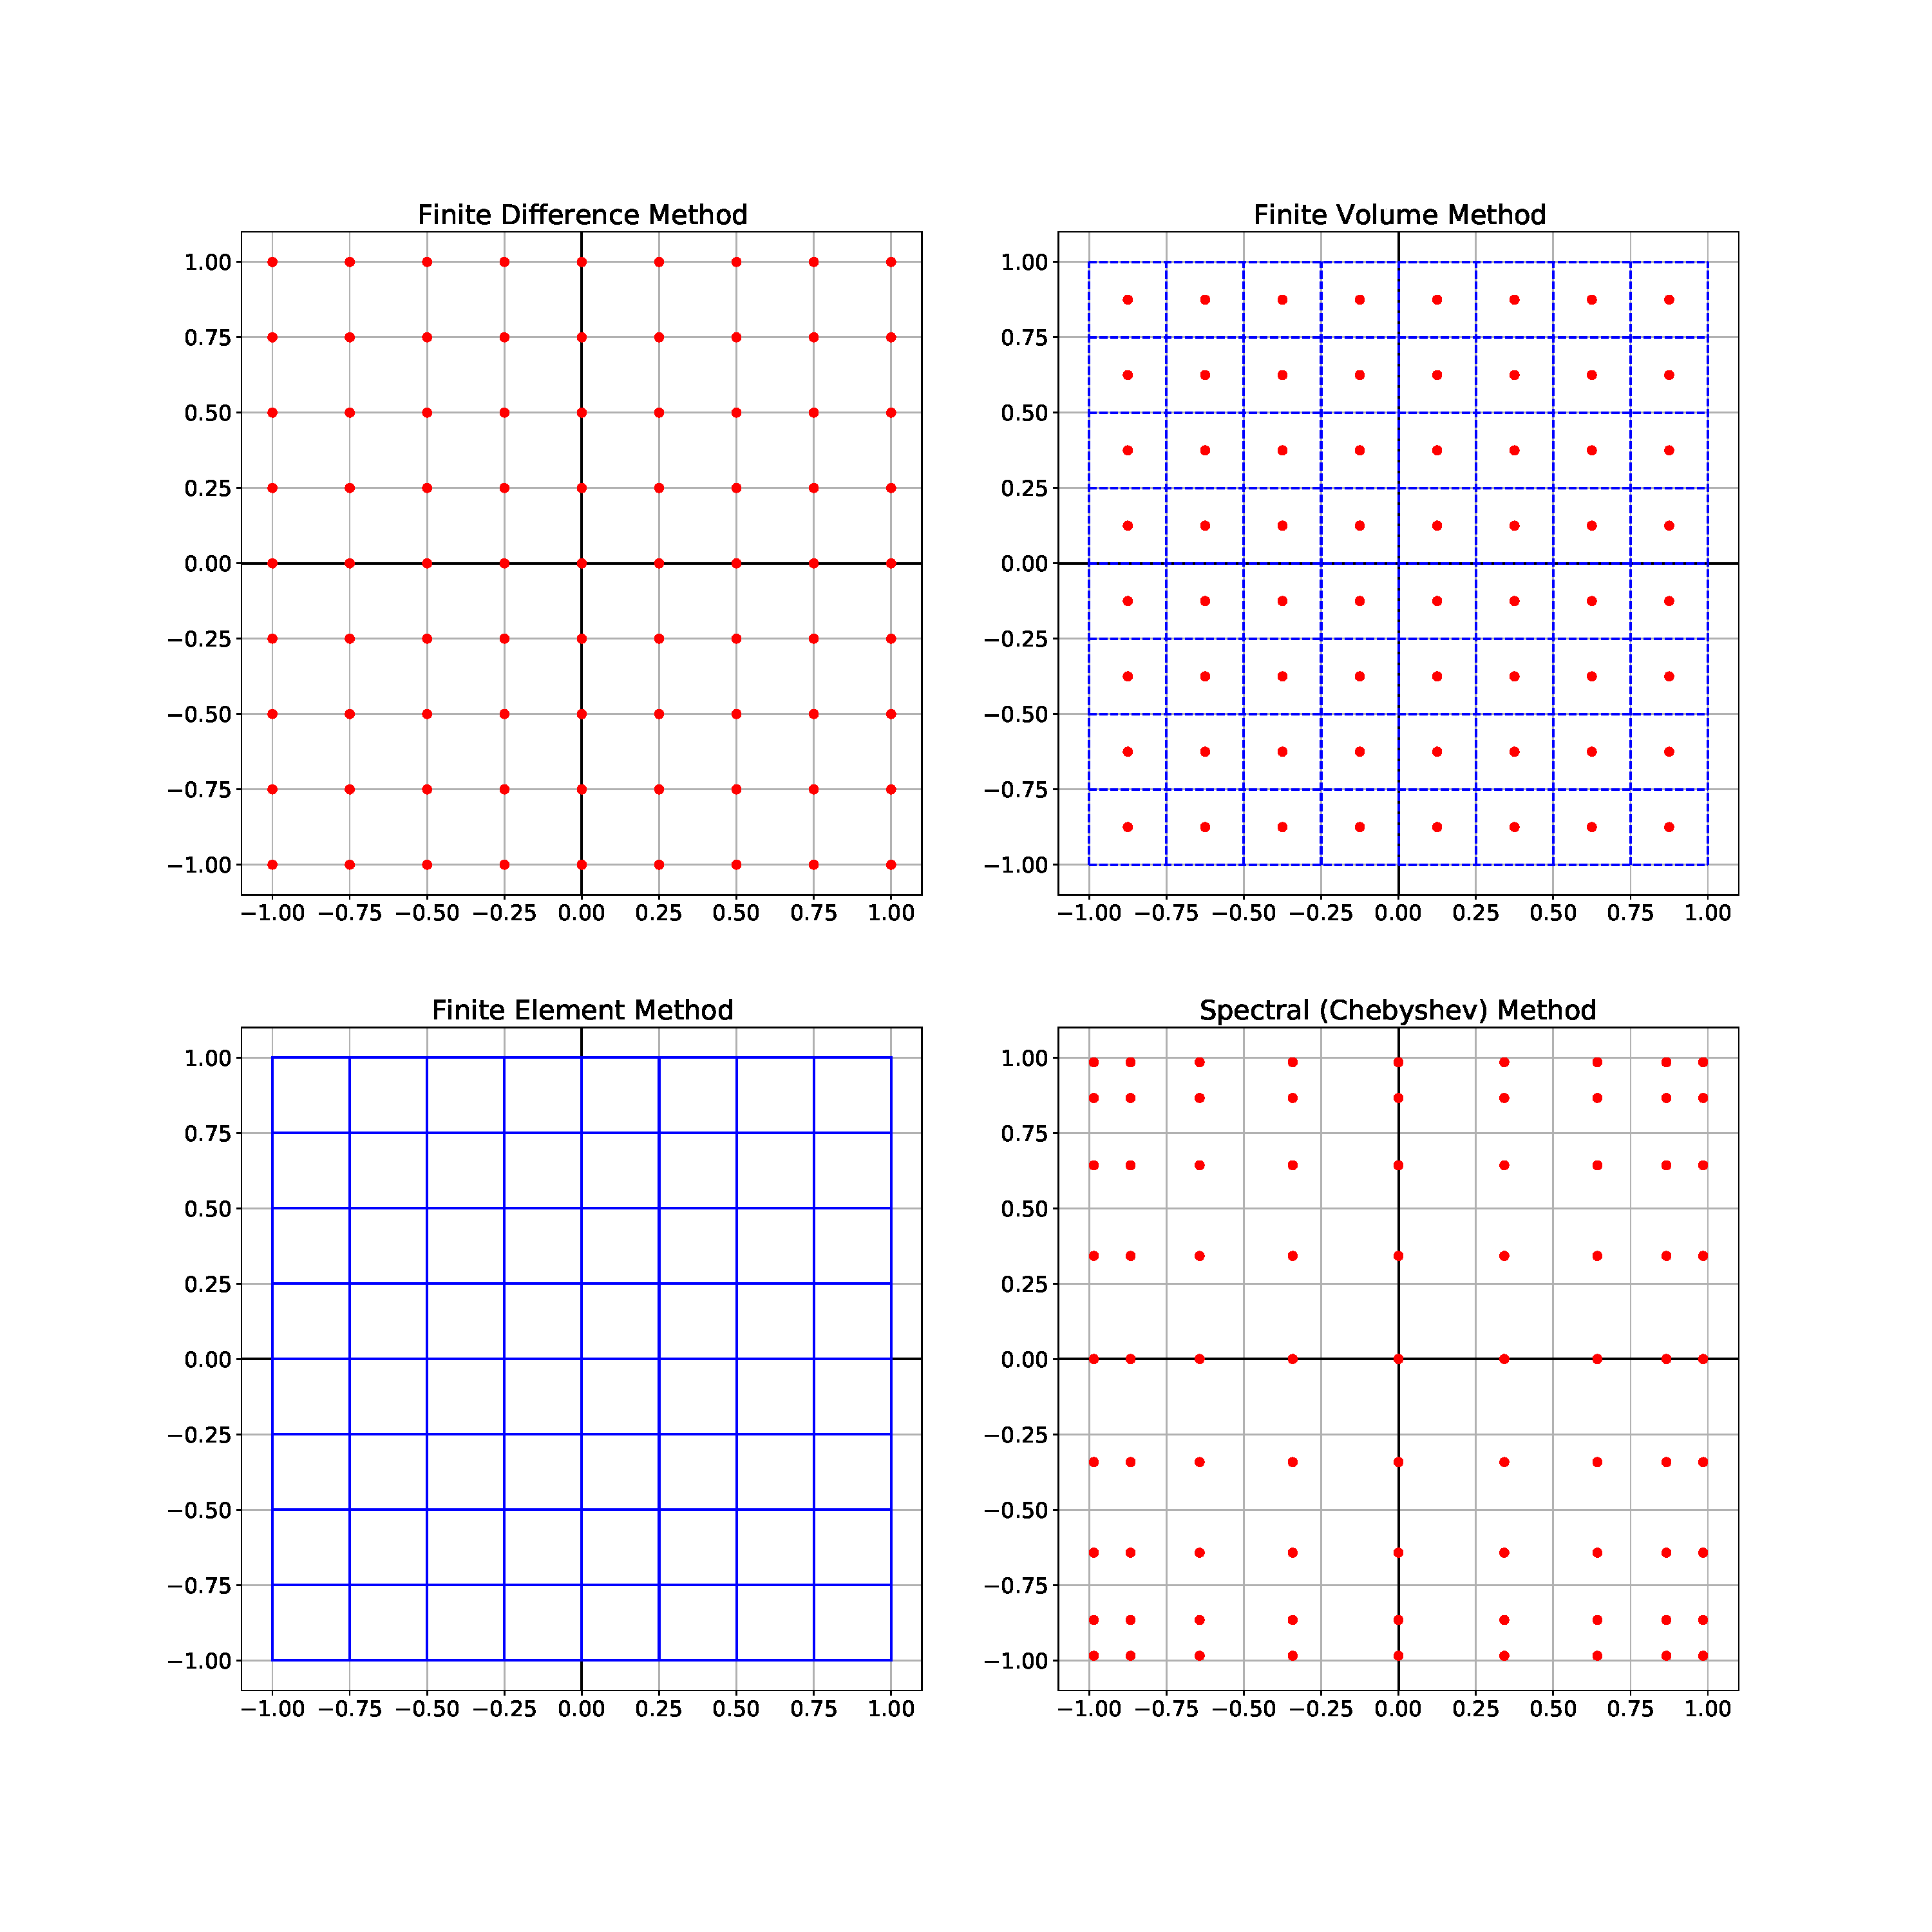
\includegraphics[width=0.8\columnwidth]{figures/PDE_discretization_methods.pdf}
    \caption{Discretization Methods. Top Left: Finite difference grid based on a mesh of points or nodes. Top Right: Finite volume mesh made of cells (dashed blue boxes) with cell averages in the center (red points). Bottom Left: Finite element mesh where each blue box is an element with a shape function defined at all points within the element. Bottom Right: Spectral mesh made up of a tensor of Chebyshev nodes.}
    \label{fig:discretization_methods}
\end{figure}

If $\Omega$ is on a logically rectangular domain (i.e. 2D Cartesian plane), perhaps the simplest discretization of the domain $\Omega$ is by collocating a mesh of points throughout the domain. Given upper and lower bounds in both directions, $[x_l, x_u], [y_l, y_u]$, the x- and y-location of each point can be defined as
\begin{align}
    x_i &= x_l + i \Delta x,\ \ \ i = 0, 1, ..., N_x-1 \\
    y_i &= y_l + j \Delta y,\ \ \ j = 0, 1, ..., N_y-1
\end{align}
where $N_x, N_y$ is the number of points in the x- and y-direction and grid spacing is defined as
\begin{align}
    \Delta x &= \frac{x_u - x_l}{N_x - 1} \\
    \Delta y &= \frac{y_u - y_l}{N_y - 1}.
\end{align}
These points are shown in the first plot of Figure \ref{fig:discretization_methods}. This type of discretization is known as the {\em finite difference method}. \damyn{(Cite something here?)}. In the finite difference approach, the expressions for the derivatives in a PDE are replaced with Taylor series approximations. For example, a second order accurate, central-difference approximation to the second derivative can be given as
\begin{align}
    \frac{\partial^2 u}{\partial x^2} &= \frac{u(x - \Delta x, y) - 2u(x, y) + u(x + \Delta x, y)}{\Delta x^2} + \mathcal{O}(\Delta x^2)
\end{align}
and if we let $u(x_i, y_j) = u_{i,j}$, then we can write this as
\begin{align}
    \frac{\partial^2 u}{\partial x^2} &= \frac{u_{i-1,j} - 2u_{i,j} + u_{i+1,j}}{\Delta x^2} + \mathcal{O}(\Delta x^2).
\end{align}
Using these Taylor Series expansions, we can replace the continuous Poisson's equation \ref{eq:variable_poisson} with the discrete system of equations:
\begin{align}
    \frac{u_{i-1,j} - 2u_{i,j} + u_{i+1,j}}{\Delta x^2} + \frac{u_{i,j-1} - 2u_{i,j} + u_{i,j+1}}{\Delta y^2} &= f_{i,j}.
    \label{eq:poisson_FD}
\end{align}
For each grid point $i = 0, ..., N_x - 1$, $j = 0, ..., N_y - 1$ this expression forms a linear system with $(N_x-1) \times (N_y-1)$ unknowns.

The system that is formed from this discretization is sparse and banded. For example, let $N_x = N_y = N$ for simplicity (thus $\Delta x = \Delta y = h$). Index the vector $\textbf{u}$ first by rows, then by columns, such that
\begin{align}
    \textbf{u} = [u_{0,0}, ..., u_{N - 1, 0}, u_{0, 1}, ..., u_{N - 1, 1}, ..., u_{0, N - 1}, ..., u_{N - 1, N - 1}]^T.
\end{align}
The corresponding linear system from \ref{eq:poisson_FD} is the following:
\begin{align}
    \textbf{A} &= \frac{1}{h^2}
    \begin{bmatrix}
        \textbf{D} & \textbf{I}_{N} & \textbf{0} & ... & \textbf{0} \\
        \textbf{I}_{N} & \textbf{D} & \textbf{I}_{N} & ... & \textbf{0} \\
        \textbf{0} & \textbf{I}_{N} & \textbf{D} & ... & \textbf{0} \\
        \vdots & \vdots & \vdots & \ddots & \vdots \\
        \textbf{0} & \textbf{0} & \textbf{0} & ... & \textbf{D}
    \end{bmatrix}
\end{align}
where
\begin{align}
    \textbf{D} &= 
    \begin{bmatrix}
        -4 & 1 & 0 & ... & 0 \\
        1 & -4 & 1 & ... & 0 \\
        0 & 1 & -4 & ... & 0 \\
        \vdots & \vdots & \vdots & \ddots & \vdots \\
        0 & 0 & 0 & ... & -4
    \end{bmatrix}.
\end{align}
We also index the RHS similarly to $u(x,y)$ resulting in a RHS vector $\textbf{f}$. This leads to the linear system
\begin{align}
    \textbf{A} \textbf{u} = \textbf{f} + \textbf{b}
\end{align}
where $\textbf{b}$ contains any updates necessary for any type of boundary condition.

\subsubsection{Finite Volume}

In a finite volume scheme, the domain is broken up into cells, which can be structured or unstructured polygons (2D) or polyhedrons (3D). The function to approximate is solved for in terms of a cell average. Finite volume schemes are often used to solve equations modeling conservation laws, where the cell quantity is conserved in time through balancing fluxes (what comes in and out of the cell boundaries) and the cell source (what the cell is generating or destroying).

Elliptic systems like the Poisson equation can be solved via the finite volume method by considering that the flux across a cell domain can be related to the quantity being advected (Fick's Law). Start with the general, linear conservation law,
\begin{align}
    \frac{\partial q(x,y,t)}{\partial t} + \nabla \cdot \textbf{F}(x,y,t) = s(x,y,t),
\end{align}
and let the flux $\textbf{F}(x,y,t)$ be related to gradient of the quantity: $\textbf{F} = \beta \nabla q$. Plugging this into the conservation equation above yields
\begin{align}
    \frac{\partial q(x,y,t)}{\partial t} + \nabla \cdot \left( \beta(x,y) \nabla q(x,y,t) \right) = s(x,y,t).
\end{align}
For the finite volume method, we integrate over the cell domain $\Omega_i$
\begin{align}
    \frac{\partial}{\partial t} \int_{\Omega_i} q(x,y,t) d\Omega_i + \int_{\Omega_i} \nabla \cdot \left( \beta(x,y) \nabla q(x,y,t) \right) d\Omega_i = \int_{\Omega_i} s(x,y,t) d\Omega_i
\end{align}
and use the divergence theorem to relate the volume integral of the flux to the surface integral of the surface:
\begin{align}
    \frac{\partial}{\partial t} \int_{\Omega_i} q(x,y,t) d\Omega_i + \int_{\Gamma_i} \beta(x,y) \nabla q(x,y,t) d\Gamma_i = \int_{\Omega_i} s(x,y,t) d\Omega_i.
\end{align}
Now, if we only consider the steady-state case ($\frac{\partial q}{\partial t} = 0$), then we get
\begin{align}
    \int_{\Gamma_i} \beta(x,y) \nabla q(x,y) d\Gamma_i = \int_{\Omega_i} s(x,y) d\Omega_i.
\end{align}

\damyn{[Finish this section; reference figure; point to finite difference stencil similarities.]}

\subsubsection{Finite Element}

In a finite element scheme, the domain is broken into elements. These elements can also be structured or unstructured polygons (2D) or polyhedrons (3D), similar to the finite volume method. The PDE to solve is converted into a weak form by multiplying the PDE by a test function $v(x,y)$ and integrating over the domain:
\begin{align}
    \int_{\Omega} v \nabla^2 u d\Omega &= \int_{\Omega} vf d\Omega.
\end{align}
Green's Theorem (i.e., integration by parts) is used to break the LHS into integrals on the domain $\Omega$ and the boundary $\partial \Omega = \Gamma$:
\begin{align}
    -\int_{\Omega} \nabla v \cdot \nabla u d\Omega + \int_{\Gamma} v \frac{\partial u}{\partial n} d\Gamma &= \int_{\Omega} vf d\Omega
    \label{eq:poisson_weak_form}
\end{align}
The idea behind the finite element method is to use basis functions
\begin{align}
    u(x,y) \approx \bar{u} = \sum_{k=1}^{N_k} c_k \phi(x,y)
\end{align}
inside each element $\Omega_i$, where $\Omega = \cup_{i = 1}^{N_{\text{elem}}} \Omega_i$. When the same basis functions for the test functions $v$ are also used, this leads to the Galerkin finite element method. Upon substitution of the above into \ref{eq:poisson_weak_form}, and integrating the basis function with either quadrature or with analytical expressions, a linear system is formed for the coefficients $c_k$.

There are several variations of the finite element method. The method explained above forms a global linear system involving all elements. To avoid this, mapping a physical element to some reference element, makes the contributions from a single element only influence itself and its neighbors. This makes the coefficient matrix in the linear system much more sparse and structured, making it easier to solve. Additionally, by not imposing continuity across element boundaries, one arrives at the discontinuous Galerkin method, where the discontinuities are handled through element fluxes. By choosing certain shape or basis functions, one can derive different variations of the finite element method, including the B-spline finite element method \citep{kagan1998new} and the spectral element method \citep{patera1984spectral}.

\subsubsection{Spectral Methods}

In spectral methods, the approach is to approximate the solution $u$ as a linear combination of a finite set of orthogonal basis functions
\begin{align}
    u(x,y) = \sum_{i=1}^{N_x} \sum_{j=1}^{N_y} c_{i,j} \phi_{i}(x) \phi_{j}(y)
\end{align}
where the coefficients are chosen to minimize a norm, such as the $L^2$ norm of the residual $r(x,y) = \nabla^2 u(x,y) - f(x,y)$. On a discrete domain, this is similar to requiring $\nabla^2 u(x_i, y_j) = f(x_i, y_j)$ at all interior grid points. As this acts like an interpolation scheme, increasing the number of discretization points on with a fixed interval actually leads to highly oscillatory results. Thus, in spectral methods, it is common to use grid points that are clustered near the ends of the interval, such as Chebyshev points, defined on an interval $[a,b]$ as
\begin{align}
    x_i &= a + \frac{1}{2}(b - a)\Big(1 + \cos \big( \pi (1 - \frac{i}{N + 1}) \big) \Big), i = 0, ..., N + 1.
\end{align}
These points are shown on the last plot of Figure \ref{fig:discretization_methods}. With a good basis of grid points, spectral methods can achieve very fast convergence. The linear system formed by this method will be dense as it functions like a high-order interpolation scheme. However, as convergence is much faster than high-order finite difference methods, one can use far fewer points on a grid, so the size of the system is kept small. If one uses Fourier series as the basis functions $\phi$, one can accelerate the solution of the linear system using fast Fourier Transform algorithms. Though, due to the periodic nature of the Fourier series, it is more difficult to implement non-periodic boundary conditions (\citep{leveque2007finite}, \citep{townsend2015automatic}).

% [TODO: Rework this section]
%
% In each of the methods presented above, the function approximation is found by forming and solving a linear system. In spectral methods, one uses integral transformations such as the Fourier or Laplace Transforms to differentiate. For example, the Fourier Transform of a function is given as
% \begin{align}
%     F(k) = \mathcal{F}[f(x)] = \frac{1}{\sqrt{2\pi}} \int_{-\infty}^{\infty} f(x) e^{ikx} dx
% \end{align}
% with it's inverse
% \begin{align}
%     f(x) = \mathcal{F}^{-1}[F(k)] = \frac{1}{\sqrt{2\pi}} \int_{-\infty}^{\infty} F(k) e^{ikx} dk.
% \end{align}
% The strength of these methods show when considering the derivatives of $f(x)$:
% \begin{align}
%     \frac{\partial^n f}{\partial x^n} &= \frac{\partial^n}{\partial x^n} \frac{1}{\sqrt{2\pi}} \int_{-\infty}^{\infty} F(k) e^{ikx} dk \\
%     &= \frac{1}{\sqrt{2\pi}} \int_{-\infty}^{\infty} (ik)^{n} F(k) e^{ikx} dk
% \end{align}
% So any $nth$ derivative can be expressed in terms of a Fourier and inverse Fourier transform:
% \begin{align}
%     \frac{\partial^n f}{\partial x^n} &= \mathcal{F}^{-1}[(ik)^n \mathcal{F}[f(x)]].
% \end{align}
% In practice, one can use fast algorithms such as the famous Fast Fourier Transform to perform this arithmetic.
%
% A minor drawback to this method is the need to work on a periodic domain in order for the Fourier Transform to function properly. This makes enforcing boundary conditions difficult. Thus, extensions to spectral methods include using a better basis of points than evenly spaced points, such as Chebyshev nodes. Chebyshev nodes defined in the interval $(-1, 1)$ are given as
% \begin{align}
%     x_k = \cos \Big( \frac{2k - 1}{2n} \pi \Big), k = 1, ..., n.
% \end{align}
% Using these nodes can increase the accurarcy of the method as well as provide a better set of collocation points for interpolation \citep{igel1999wave}.

\subsubsection{Other Methods and Summary}

These methods are not all the possible ways to solve an elliptic PDE. Other methods include using quadrature methods on the integral formulation of the PDE, as well as collocation methods such as radial basis function approximations. However, the methods we reviewed show some of the most classic approaches to solving elliptic PDEs.

\subsection{Solution Methods for Elliptic Partial Differential Equations}
\label{sec:solution-methods-for-elliptic-pdes}

The discretization methods described in \refsec{sec:numerical-methods-for-elliptic-pdes} result in a linear system. To generally talk about these solution methods, we assume that we form the linear system
\begin{align}
    \textbf{A} \textbf{u} = \textbf{b}
    \label{eq:ls}
\end{align}
where $\textbf{A} \in \mathbb{R}^{N \times N}$ is a coefficient matrix formed from one of the discretization methods, $N$ is the number of degrees of freedom, $\textbf{u} = u_i = u(x_i)$ for $i \in \textbf{I}_x$, index set $\textbf{I}_x$ for the discrete domain, and $\textbf{b}$ is the right-hand side vector encoded with the boundary conditions and the inhomogeneous function $f(\textbf{x})$. The goal is to solve for $\textbf{u}$ where we take advantage of the sparsity and structure of $\textbf{A}$. We organize the various methods into the following three categories: 1) iterative methods, 2) direct methods, and 3) hierarchical methods.

\subsubsection{Iterative Methods}
\label{sub:iterative-methods}

Iterative methods start with an initial guess of a solution to \ref{eq:ls} and correct the iterate until convergence to a specified tolerance. The simplest iterative methods are called splitting methods where the linear system is modified according to
\begin{align}
\textbf{A} = \textbf{M} - \textbf{N} \Rightarrow \textbf{M} \textbf{u} = \textbf{N} \textbf{u} + \textbf{b}.
\end{align}
This suggests the following recursion relationship for the next iteration:
\begin{align}
\textbf{M} \textbf{u}^{k+1} &= \textbf{N} \textbf{u}^k + \textbf{b} \\
\textbf{u}^{k+1} &= \textbf{M}^{-1} \textbf{N} \textbf{u}^k + \textbf{M}^{-1} \textbf{b}.
\end{align}
The idea is to choose $\textbf{M}$ that captures as much of $\textbf{A}$ as possible, but is still easy and quick to invert. As $\textbf{A}$ is either banded or sparse, classical splitting methods for elliptic PDEs split $\textbf{A}$ into $\textbf{A} = \textbf{D} - \textbf{L} - \textbf{U}$, where $\textbf{D}$ is the diagonal components of $\textbf{A}$, and $\textbf{L}$ and $\textbf{U}$ are the lower and upper pieces, respectively. Classical choices for $\textbf{M}$ and $\textbf{N}$ are summarized in Table \ref{tab:splitting}.

\begin{table}[h!]
    \centering
    \begin{tabular}{ | l | l | l |}
        \hline
        Jacobi & $\textbf{M} = \textbf{D}$ & $\textbf{N} = \textbf{L} + \textbf{U}$ \\
        Gauss-Sidel & $\textbf{M} = \textbf{D} - \textbf{L}$ & $\textbf{N} = \textbf{U}$ \\
        Successive Over Relaxation & $\textbf{M} = \frac{1}{\omega}(\textbf{D} - \omega \textbf{L})$ & $\textbf{N} = \frac{1}{\omega} \big( (1 - \omega) \textbf{D} + \omega \textbf{U} \big)$ \\
        \hline
    \end{tabular}
    \caption{Iterative Methods: Splitting Methods}
    \label{tab:splitting}
\end{table}

Another class of iterative methods are called Krylov subspace methods. The Krylov space is defined as
\begin{align}
\mathcal{K}_k = \text{span} \{ \textbf{r}_0, \textbf{A} \textbf{r}_0, \textbf{A}^2 \textbf{r}_0, ..., \textbf{A}^{k-1} \textbf{r}_0 \}
\end{align}
based on the initial residual $\textbf{r}_0 = \textbf{b} - \textbf{A} \textbf{u}^{(0)}$. The goal is to take the next iteration from this particular space. Two common Krylov methods are the Conjugate Gradient method \citep{hestenes1952methods} and the Generalized Minimal Residual (GMRES) method \citep{saad1986gmres}. In the conjugate gradient method, the approximation is adjusted by a conjugate direction, or a vector that is conjugate with respect to $\textbf{A}$. This vector is called the search direction $\textbf{p}$ and is scaled by $\alpha$, which is computed by solving a quadratic minimization problem. The GMRES method builds up an orthogonal matrix $\textbf{Q}$ through a process called the Arnoldi iteration. The Arnoldi iteration forms $\textbf{A} = \textbf{Q} \textbf{H} \textbf{Q}^*$ for orthogonal matrix $\textbf{Q}$ and Hessenberg matrix $\textbf{H}$. The next iteration is found via $\textbf{Q} \textbf{y}$ where $\textbf{y}$ is found from a least squares problem involving $\textbf{H}$. These methods are summarized in Table \ref{tab:ksm}.

\begin{table}[h!]
    \centering
    \begin{tabular}{ | l | l |}
        \hline
        Conjugate Gradient & $\textbf{u}^{(k+1)} = \textbf{u}^{(k)} + \alpha^{(k)} \textbf{p}^{(k)}$ \\
        GMRES & $\textbf{u}^{(k)} = \textbf{Q}^{(k)} \textbf{y}$ \\
        \hline
    \end{tabular}
    \caption{Iterative Methods: Krylov Subspace Methods}
    \label{tab:ksm}
\end{table}

Most iterative methods are considered ``matrix-free" methods. A ``matrix-free" method is a method that does not explicitly form the matrix $\textbf{A}$, but is rather applied to a vector. For example, if implementing a Conjugate Gradient method for a finite difference discretization, one has to compute the product $\textbf{A} \textbf{u}^{(k)}$. Instead of doing the full matrix-vector calculation, one can write a function that takes $\textbf{u}$ and returns the 2nd-order, central difference operator as computed in \ref{eq:poisson_FD}.

As finite difference discretization schemes for elliptic PDEs lead to sparse matrices, the application of $\textbf{A}$ to a vector can be done in $\mathcal{O}(N)$ operations, where $N$ is the number of unknowns in the vector. Thus, the performance for most iterative methods is approximately $\mathcal{O}(N \times N_{iter})$, where $N_{iter}$ is the number of iterations required for a specified tolerance. However, as $N$ gets larger, often so does $N_{iter}$, leading to poor scaling, as noted in \citep{martinsson2019fast}. In addition, iterative methods may not always converge for a given initial guess or structure of $\textbf{A}$, which make them unfavorable for ``black-box" implementations for linear solvers.

\subsubsection{Direct Methods}
\label{sub:direct-methods}

Motivation for direct solvers stems from wanting to improve upon the disadvantages of iterative methods. Martinsson notes in \citep{martinsson2004fast} some advantages to using direct methods over iterative ones:
\begin{itemize}
    \item Direct methods can be applied to multiple right-hand side vectors $\textbf{b}$ or multiple boundary conditions once a factorization or solution operator is built, whereas iterative methods must be solved anew for each right-hand side or for different boundary conditions.

    \item Direct methods can take advantage of ``close" matrices (i.e. if we have an inverse or factorization of $\textbf{A}$ and perturb it by $\epsilon$, we could adjust the inverse to account for it instead of recompute the inverse).

    \item Most direct methods can take advantage of fast and efficient algorithms for matrix factorization such as the singular value decomposition, LU decomposition, QR decomposition, etc.
\end{itemize}
We will look at how direct methods are useful as we consider some common direct methods from \citep{leveque2007finite} and \citep{trefethen1997numerical}.

Many direct methods are based on matrix factorizations. Perhaps the most well-known is the LU decomposition. LU decomposition factors the coefficient matrix into a lower and upper triangular matrix: $\textbf{A} = \textbf{L} \textbf{U}$. The idea is to use Gaussian elimination to eliminate entries below the main diagonal, and then use back-substitution to solve for each entry in $\textbf{u}$. In general, LU decomposition requires $\mathcal{O}(N^3)$ floating point operations and thus is impractical for large matrices. There are banded solvers for Gaussian elimination that can take advantage of the sparsity of a matrix. The Cholesky decomposition is a variant of Gaussian elimination for symmetric matrices. Other matrix factorizations include the QR-decomposition, $\textbf{A} = \textbf{Q} \textbf{R}$, and the singular value decomposition, $\textbf{A} = \textbf{U} \boldsymbol{\Sigma} \textbf{V}^*$.

For a finite difference discretization of elliptic PDEs, $\textbf{A}$ is banded and sparse, and more efficient algorithms for LU decomposition exist. For 1D problems, $\textbf{A}$ is diagonally dominant and sparse with the bandwidth (the number of entries off the main diagonal in a matrix) dependent on the order of the stencil. For the stencil shown in the second order discretization in \ref{eq:poisson_FD}, $\textbf{A}$ is tridiagonal. This allows us to use algorithms such as Thomas's algorithm for solving a tridiagonal system in $\mathcal{O}(N)$ steps (\citep{higham2002accuracy}). In higher dimensions, block versions of Thomas's algorithm exist (\citep{quarteroni2010numerical}).

Compared to iterative methods, direct methods will terminate in a finite number of steps. Direct methods are more fit for ``black-box" implementations. However, because most direct methods need to explicitly form $\textbf{A}$, they are more difficult to implement with limited computing resources. Indeed, going to higher dimensions and higher orders often dramatically increases memory and compute requirements.

\subsubsection{Hierarchical Methods}
\label{sub:hierarchical-methods}

The methods grouped under hierarchical methods attempt to accelerate some of the ideas from iterative and direct methods by breaking the problem into a hierarchy of subproblems. By recursively breaking the original problem into smaller subproblems, significant improvements can be made in complexity and performance. We'll talk about three hierarchical methods here: the multigrid method, nested dissection, and the Hierarchical Poincaré-Steklov (HPS) method.

\subsubsection{The Multigrid Method}
\label{subsub:multigrid-method}

The multigrid method was introduced by Brandt in \citep{brandt1977multi}. It has been widely used in various applications and for all types of solution methods. Briggs in \citep{briggs2000multigrid} gives an overview and tutorial of the multigrid method.

In the multigrid method, the idea is to use multiple levels of grids and solution methods on each level to solve a larger problem. To look at the multigrid method, we define the error in the linear system to be $\textbf{e} = \textbf{u}^{(k)} - \textbf{u}_{exact}$ (the difference between the exact solution and the $kth$ iteration). After a few iterations of a smoother (typically Jacobi's method), because of the local averaging, any high-frequency error is quickly dampened away. What takes longer to eliminate is the low-frequency error associated with the global problem. By coarsening the grid, the lower frequency error is dampened quicker. Multigrid combines the ability of iterative methods to locally reduce error and a coarsening grid technique to accelerate convergence.

In the multigrid method, one starts with the solution on a fine grid, for example, with grid spacing $h$, and performs a few iterations of a smoother. After a few iterations, the $h$-level grid is projected onto a coarser $2h$-level grid. On this level, one performs a few more iterations of a smoother. Because the grid is coarser, this step is faster. Again, after a few iterations, the solution is projected onto an even coarser $4h$-level grid and a few more iterations are performed. This is done a specified number of times, and then the solution is interpolated back up the levels to the original grid. This is shown in Figure \ref{fig:multigrid}.

\begin{figure}
    \centering
    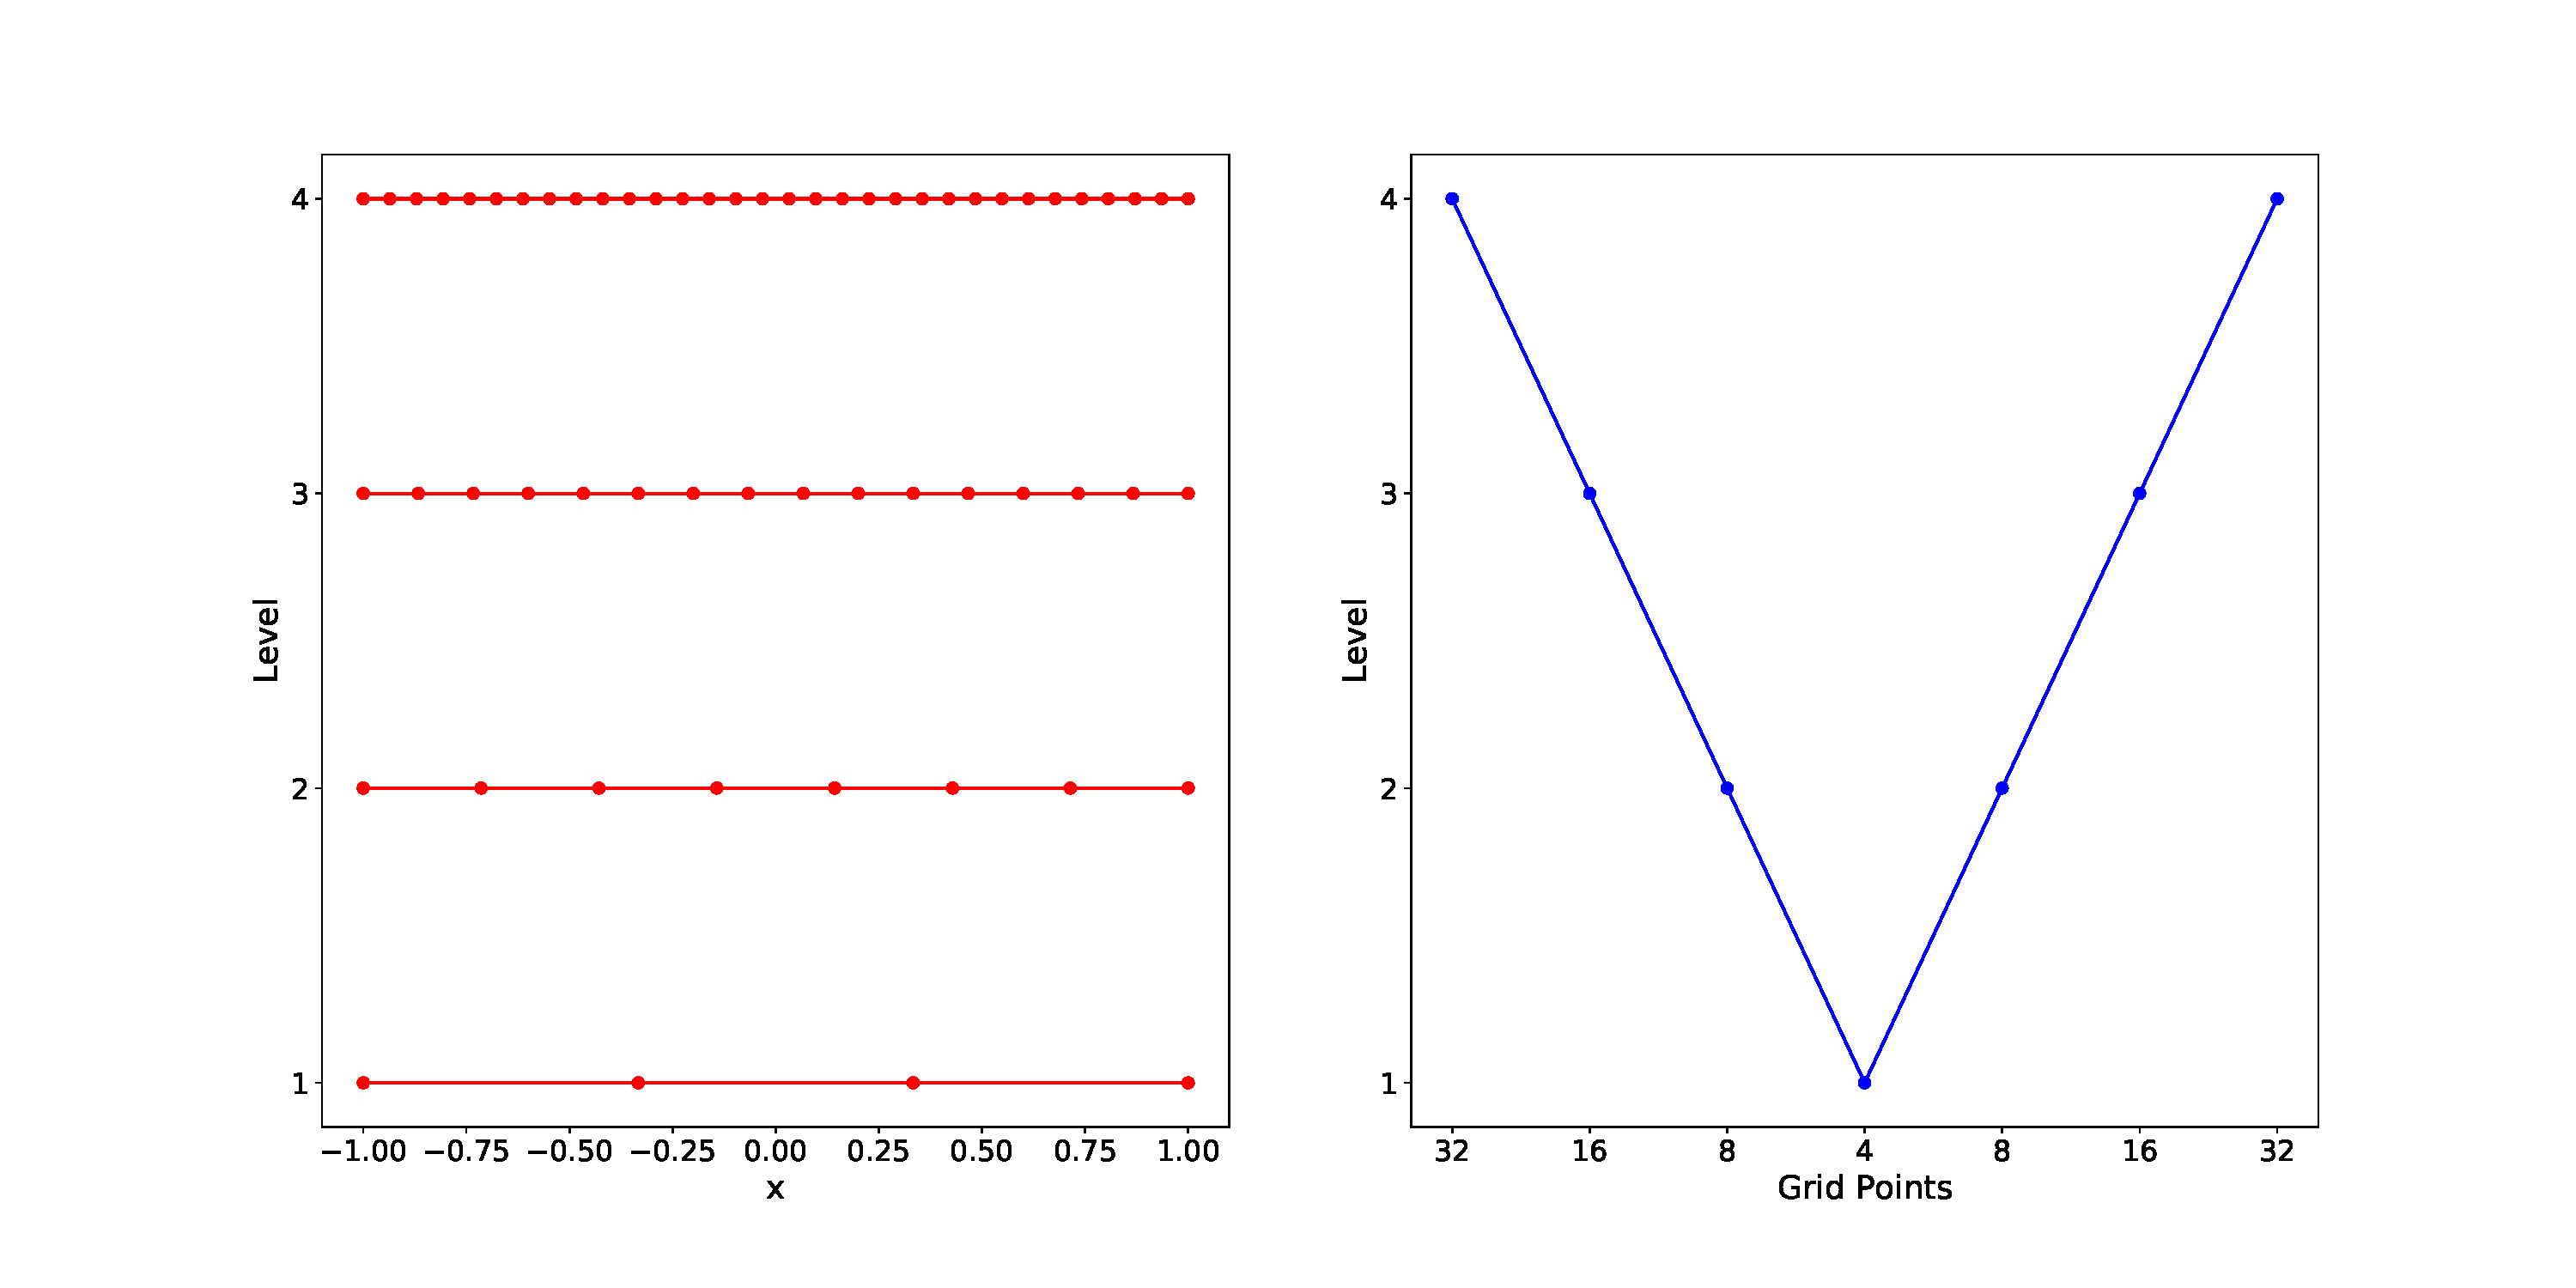
\includegraphics[width=0.8\columnwidth]{figures/multigrid.pdf}
    \caption{The 1D Multigrid Method. Starting with the finest grid, perform a few iterations of an iterative method. This is called relaxing the solution. Then project onto a coarser grid, and relax again. Do this down the levels in the grid to a desired precision. Once the solution is converged to on the coarsest level, interpolate back up the levels to obtain the solution on the finest level.}
    \label{fig:multigrid}
\end{figure}

In what is called the ``full multigrid" method, the process starts on the coarsest level instead of the finest. The solution is relaxed on this level, and then interpolated down onto a finer mesh. The interpolated solution is used as an initial guess for solving the problem on the finer mesh. The relaxed solution on a coarser grid is often an ideal initial guess for the problem on the finer mesh, resulting in quick convergence on that level.

The multigrid method allows one to accelerate an iterative solver. Multigrid methods are very effective as pre-conditioners for iterative methods. This is the general pattern of hierarchical methods: the ability to use classical iterative and direct methods on smaller grids where they perform well, and then ``scale" them up to larger problem sizes.

\subsubsection{Nested Dissection}
\label{subsub:nested-dissection}

The nested dissection method formulated by George in \citep{george1973nested} is a direct method that builds upon Gaussian elimination for problems on a grid. It is also the basis for forming what is called the multifrontal method. By taking advantage of the ordering of points on a grid, one can permute $\textbf{A}$ to first eliminate points that split the mesh into two unconnected meshes. This permutation takes the form of $\textbf{P}^* \textbf{A} \textbf{P}$, where the goal is to form $\textbf{P}$ to reorganize $\textbf{A}$ in a way that eliminates points in an efficient manner.

To detail nested dissection better, consider an $N \times N$ mesh such as a finite difference mesh discussed in Section \ref{sec:elliptic}. Assume that the initial ordering of points corresponds to an index set that iterates over the points in the mesh row-by-row. Now, the idea of nested dissection is to reorganize the points such that we first eliminate points down the middle of the mesh (i.e. the points at $x = 0$ in the first plot of Figure \ref{fig:discretization_methods}). Once these points are solved for, it spilts the mesh into two equally sized pieces that are disconnected. Each of the disconnected meshes now are smaller, and thus easier to solve. This idea of splitting the mesh into disconnected pieces by first eliminating points along an interface can be recursively applied to each split. This means that after dividing the mesh into two, one can divide those two meshes into four meshes, and so on. Recursive splitting is a common characteristic in hierarchical methods.

Nested dissection was first introduced by George in \citep{george1973nested}, and further generalized by Lipton et al. in \citep{lipton1979generalized}. Martinsson has a tutorial on nested dissection in \citep{martinsson2019fast}. In fact, nested dissection served as motivation for another hierarchical method proposed by Martinsson and Gillman called the Hierarchical Poincaré-Steklov method.

\subsubsection{The Hierarchical Poincaré-Steklov Method}
\label{subsub:hps-method}

The work done by Gillman and Martinsson in \citep{martinsson2004fast}, \citep{MARTINSSON2013460}, and \citep{gillman2014direct} (with a practical tutorial found in \citep{martinsson2015hierarchical}) culminate in what they call the Hierarchical Poincaré-Steklov (HPS) method. It is a direct solver for elliptic PDEs that is based on a binary tree of rectangular patches where the solution operator to $\textbf{A}$ is built by recursively merging child patches. Like direct methods, the HPS method involves a factorization step and a solve step. The chief advantage of the HPS method over other direct methods is that it does not require the explicit formulation and storage of $\textbf{A}$.

The HPS method starts with an original problem domain, and recursively divides the domain in half. This creates a binary tree of patches as shown in Figure \ref{fig:solve}. Once the domain has been decomposed into this tree of patches, two operators are defined on the lowest level, called the leaf level. These operators are the solution operator $\textbf{S}$ and Dirichlet-to-Neumann (DtN) operator $\textbf{T}$. The solution operator maps boundary data to solution data on the interior of the patch (i.e. solves the local boundary value problem), and the DtN operator maps Dirichlet data on the boundary to Neumann data on the boundary. These operators can be formed using any elliptic PDE solver, including fast solvers like spectral methods. After forming these operators, the next step is to recursively merge each sibling patch up the tree. the merge step is demonstrated in Figure \ref{fig:merge}. This results in a global solution operator that can be stored and used multiple times (at different time steps or with varying boundary conditions, etc.), and is similar to a direct method matrix factorization. The final step is applying the solution operator to each level down the tree to obtain the solution everywhere in the domain. This step is just a matrix-vector multiplication and is very fast.

Similar to other direct methods, the HPS method forms an in-memory solution operator that can be applied to several right-hand side vectors. This property makes it ideal for problems where several elliptic solves are necessary. While most iterative methods have better asymptotic performance than other direct methods, the HPS method can be accelerated using hierarchically block seperable (HBS) matrix algebra to achieve near linear asymptotic performance (\citep{gillman2014direct}).

\begin{figure}
    \centering
    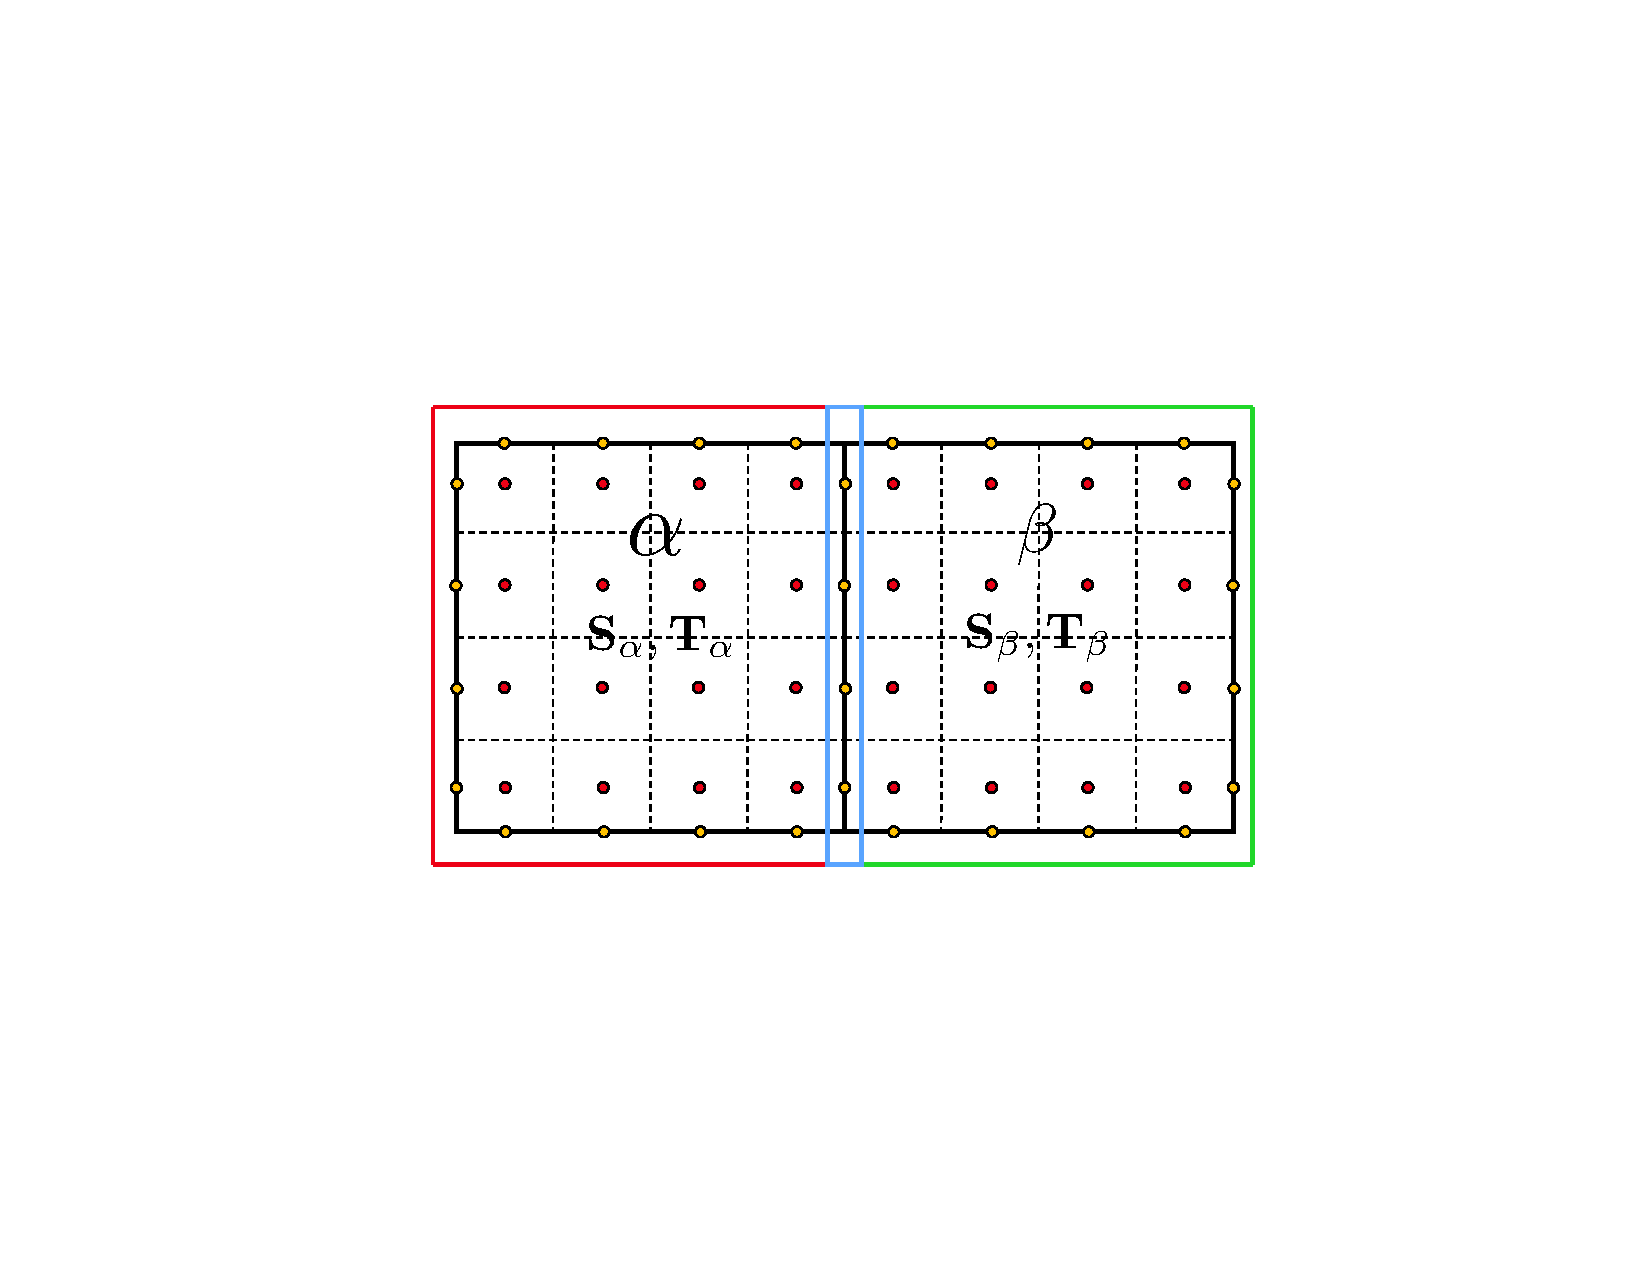
\includegraphics[width=0.7\columnwidth]{figures/merge_figure.pdf}
    \caption{HPS Merge Operation. The merged patch $\Omega_{\tau}$ is the union of children $\Omega_{\alpha}$ and $\Omega_{\beta}$, i.e. $\Omega_{\tau} = \Omega_{\alpha} \cup \Omega_{\beta}$. Red, green, and blue nodes correspond to index sets $\textbf{I}_1$, $\textbf{I}_2$, and $\textbf{I}_3$, respectively. The merge operation eliminates the nodes on the interface of the children patches.}
    \label{fig:merge}
\end{figure}

\begin{figure}
    \centering
    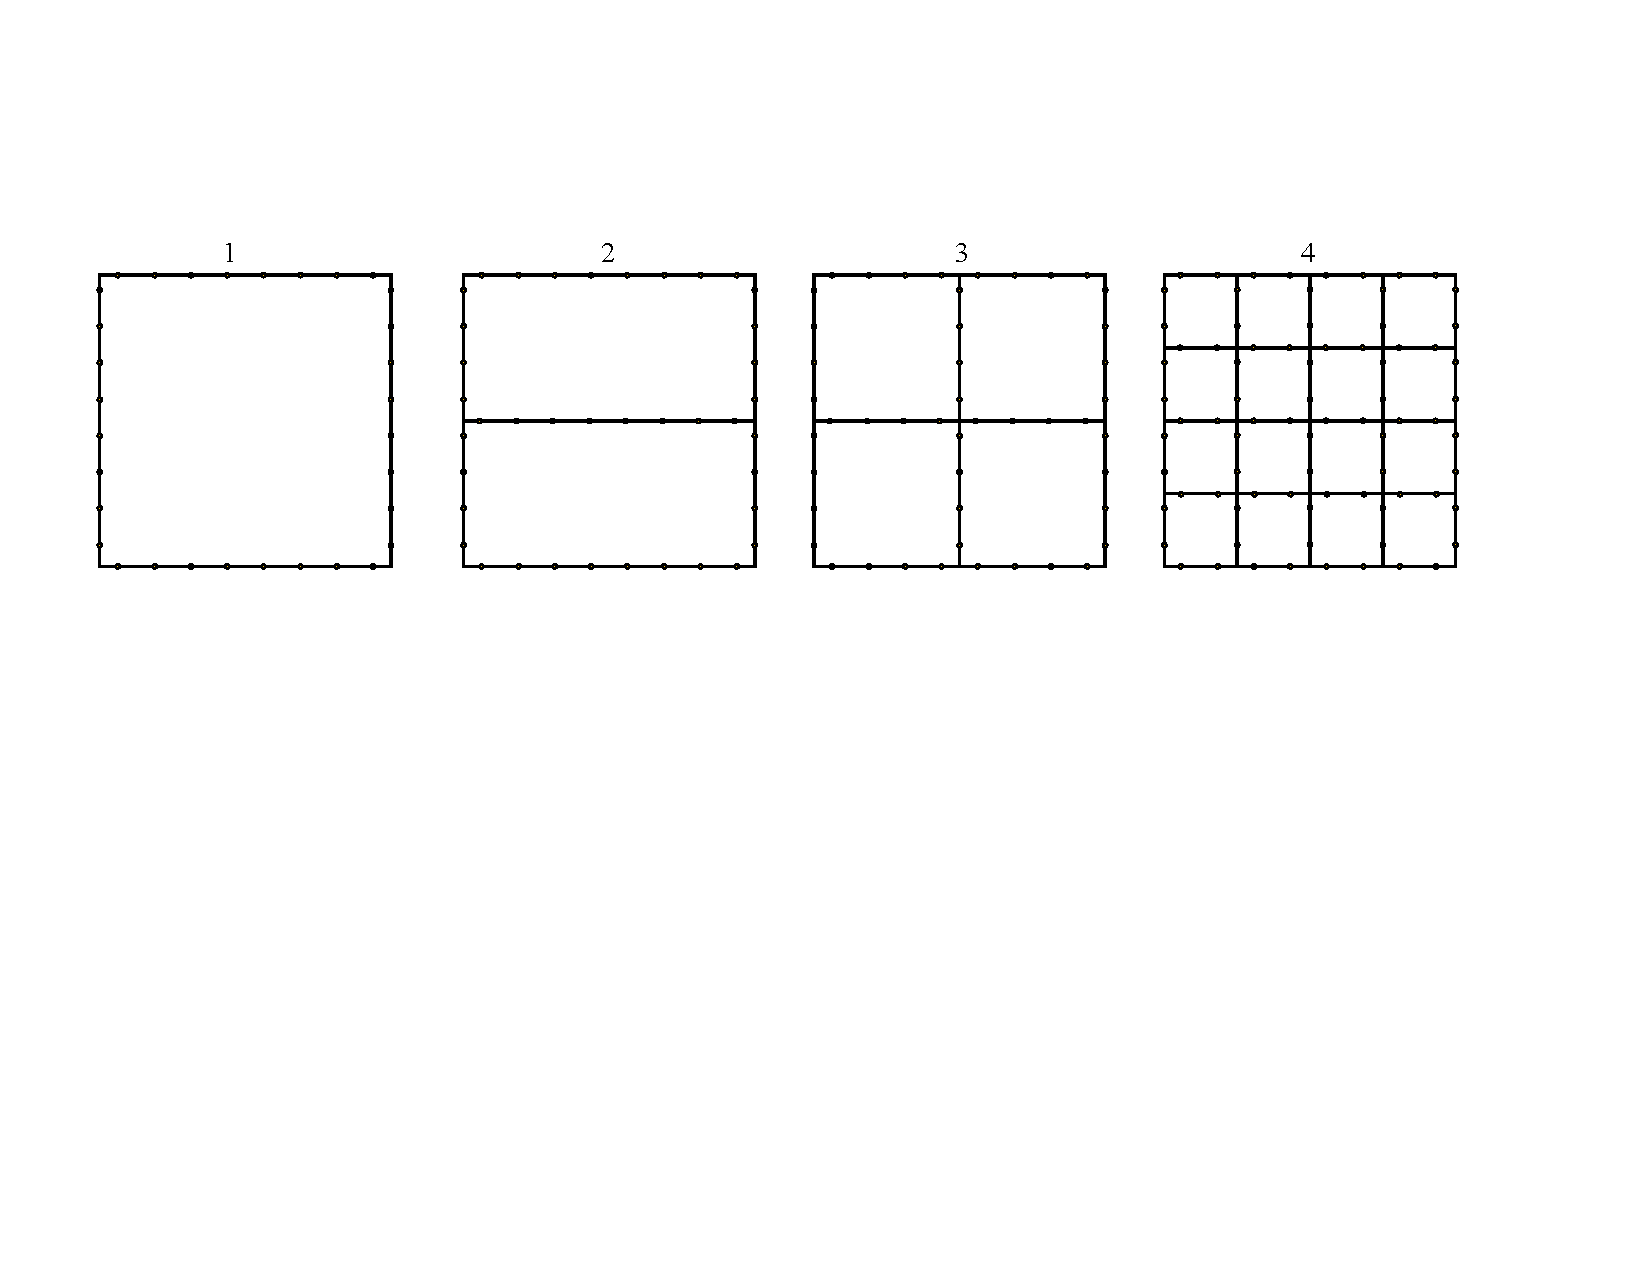
\includegraphics[width=\columnwidth]{figures/solve_figure.pdf}
    \caption{HPS Solve Stage. Once $\textbf{S}_0$ is formed, apply it to the top level Dirichlet data to get boundary (and solution) data on the interface of the children. Apply the patch solution operator down the tree until each leaf has it's local boundary information. Then apply the solution operator to get the solution data in the interior of each leaf.}
    \label{fig:solve}
\end{figure}

\section{Literature Review}
\label{sec:lit-review}

\subsection{The Elliptic Partial Differential Equation}

Partial differential equations are classified by their highest order derivative terms. A second order, linear differential equation can be written as
\begin{align*}
    A(\textbf{x}) \frac{\partial^2 u(\textbf{x})}{\partial x^2} + B(\textbf{x}) \frac{\partial^2 u(\textbf{x})}{\partial x \partial y} + C(\textbf{x}) \frac{\partial^2 u(\textbf{x})}{\partial y^2} + ... \\
    ... + D(\textbf{x}) \frac{\partial u(\textbf{x})}{\partial x} + E(\textbf{x}) \frac{\partial u(\textbf{x})}{\partial y} + F(\textbf{x}) u(\textbf{x}) + G(\textbf{x}) &= 0.
\end{align*}
Second order linear PDEs are classified according to the value of the determinant: 
\begin{align*}
    B^2 - 4AC &< 0,\ \ \ \text{Elliptic} \\
    B^2 - 4AC &= 0,\ \ \ \text{Parabolic} \\
    B^2 - 4AC &> 0,\ \ \ \text{Hyperbolic}
\end{align*}

In this overview, we will consider common elliptic PDEs such as the Poisson equation
\begin{align}
    \nabla \cdot \left( \beta(\textbf{x}) \nabla u(\textbf{x}) \right) &= f(\textbf{x}),
    \label{eq:variable_poisson}
\end{align}
and the Helmholtz equation
\begin{align}
    \nabla \cdot \left( \beta(\textbf{x}) \nabla u(\textbf{x}) \right) + \lambda(\textbf{x}) u(\textbf{x}) &= f(\textbf{x}),
    \label{eq:variable_helmholtz}
\end{align}
where $\textbf{x} = [x, y]$, $\nabla = (\frac{\partial}{\partial x}, \frac{\partial}{\partial y})$, $\nabla^2 = \nabla \cdot \nabla = \frac{\partial^2}{\partial x^2} + \frac{\partial^2}{\partial y^2}$, and $\textbf{x} \in \Omega \subset \mathbb{R}^2$. When $\beta(\textbf{x}) = 1$ and $\lambda(\textbf{x}) = \kappa^2$ ($\kappa$ is a constant), these expressions reduce to the more classical, constant coefficient versions of the Poisson and Helmholtz equations. When the right-hand side function $f(\textbf{x}) = 0$, these are homogeneous problems, where \refeqn{eq:variable_poisson} is reduced to the Laplace equation. Each of these PDEs are subject to the appropriate boundary conditions on the domain boundary $\partial \Omega = \Gamma$. Such boundary conditions (BCs) can either be Dirichlet (Type-I), Neumann (Type-II), or Robin/Mixed (Type-III) BCs. Dirichlet problems impose the value of $u$ on the boundaries, Neumann problems impose the flux or normal gradient $\partial_n u$ on the boundaries, while Robin problems impose a linear combination of Dirichlet and Neumann type BCs.

Although analytical solutions exist for some simple variations of the problems above, we are interested in looking at numerical methods to solve these equations. To do so, we look at various ways to discretize the domain $\Omega$. This discretization will lead to a linear system of equations which we will solve with numerical methods, taking advantage of the sparsity and structure of the associated system.

\subsection{Classic Numerical Methods}
\label{sec:numerical-methods-for-elliptic-pdes}

\subsubsection{Finite Difference}
\label{subsub:finite-difference}

\begin{figure}
    \centering
    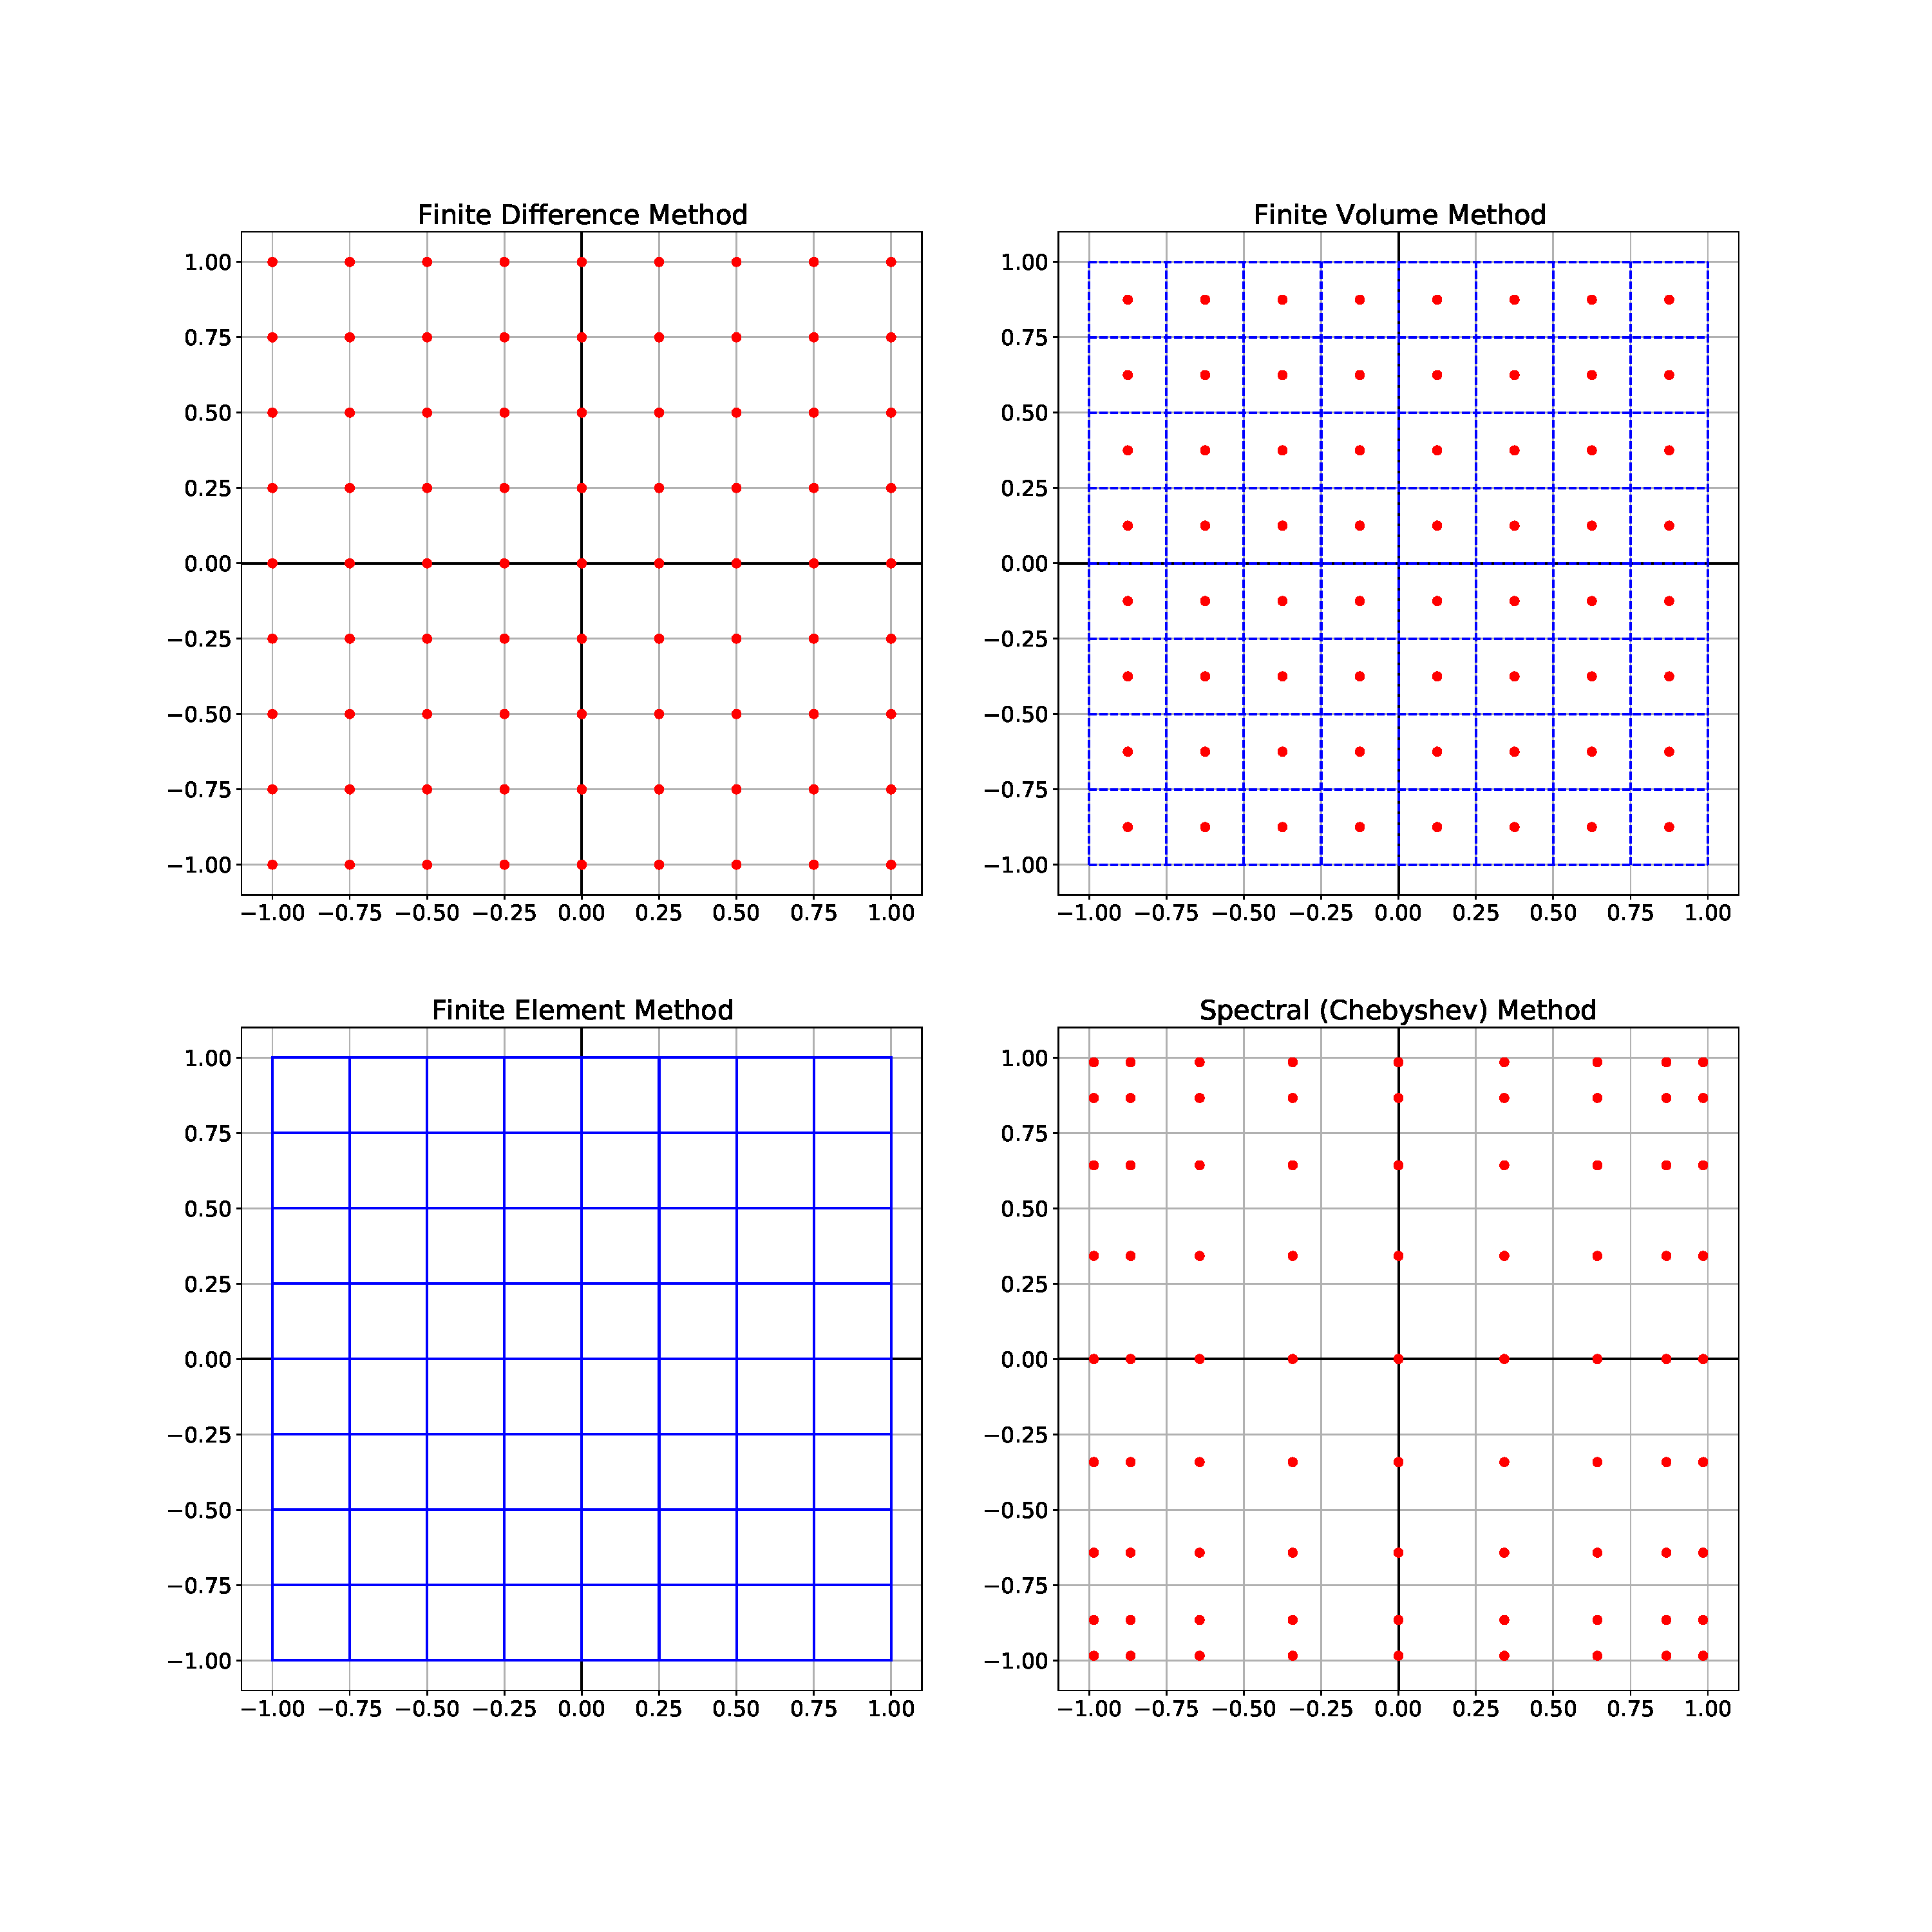
\includegraphics[width=0.8\columnwidth]{figures/PDE_discretization_methods.pdf}
    \caption{Discretization Methods. Top Left: Finite difference grid based on a mesh of points or nodes. Top Right: Finite volume mesh made of cells (dashed blue boxes) with cell averages in the center (red points). Bottom Left: Finite element mesh where each blue box is an element with a shape function defined at all points within the element. Bottom Right: Spectral mesh made up of a tensor of Chebyshev nodes.}
    \label{fig:discretization_methods}
\end{figure}

If $\Omega$ is on a logically rectangular domain (i.e. 2D Cartesian plane), perhaps the simplest discretization of the domain $\Omega$ is by collocating a mesh of points throughout the domain. Given upper and lower bounds in both directions, $[x_l, x_u], [y_l, y_u]$, the x- and y-location of each point can be defined as
\begin{align}
    x_i &= x_l + i \Delta x,\ \ \ i = 0, 1, ..., N_x-1 \\
    y_i &= y_l + j \Delta y,\ \ \ j = 0, 1, ..., N_y-1
\end{align}
where $N_x, N_y$ is the number of points in the x- and y-direction and grid spacing is defined as
\begin{align}
    \Delta x &= \frac{x_u - x_l}{N_x - 1} \\
    \Delta y &= \frac{y_u - y_l}{N_y - 1}.
\end{align}
These points are shown in the first plot of Figure \ref{fig:discretization_methods}. This type of discretization is known as the {\em finite difference method}. In the finite difference approach, the expressions for the derivatives in a PDE are replaced with Taylor series approximations. For example, a second order accurate, central-difference approximation to the second derivative can be given as
\begin{align}
    \frac{\partial^2 u}{\partial x^2} &= \frac{u(x - \Delta x, y) - 2u(x, y) + u(x + \Delta x, y)}{\Delta x^2} + \mathcal{O}(\Delta x^2)
\end{align}
and if we let $u(x_i, y_j) = u_{i,j}$, then we can write this as
\begin{align}
    \frac{\partial^2 u}{\partial x^2} &= \frac{u_{i-1,j} - 2u_{i,j} + u_{i+1,j}}{\Delta x^2} + \mathcal{O}(\Delta x^2).
\end{align}
Using these Taylor Series expansions (and $\beta(x,y) = 1$), we can replace \refeqn{eq:variable_poisson} with the discrete system of equations:
\begin{align}
    \frac{u_{i-1,j} - 2u_{i,j} + u_{i+1,j}}{\Delta x^2} + \frac{u_{i,j-1} - 2u_{i,j} + u_{i,j+1}}{\Delta y^2} &= f_{i,j}.
    \label{eq:poisson_FD}
\end{align}
For each grid point $i = 0, ..., N_x - 1$ and $j = 0, ..., N_y - 1$, this expression forms a linear system with $(N_x-1) \times (N_y-1)$ unknowns. The system that is formed from this discretization is sparse and banded. When $\beta(\textbf{x}) > 0$, the system formed by this discretization is also symmetric, positive definite (SPD). This allows the use of more optimized solvers such as the Conjugate Gradient method.

For example, let $N_x = N_y = N$ for simplicity (thus $\Delta x = \Delta y = h$). Index the vector $\textbf{u}$ first by rows, then by columns, such that
\begin{align}
    \textbf{u} = [u_{0,0}, ..., u_{N - 1, 0}, u_{0, 1}, ..., u_{N - 1, 1}, ..., u_{0, N - 1}, ..., u_{N - 1, N - 1}]^T.
\end{align}
The corresponding linear system from \refeqn{eq:poisson_FD} is the following:
\begin{align}
    \textbf{A} &= \frac{1}{h^2}
    \begin{bmatrix}
        \textbf{D} & \textbf{I}_{N} & \textbf{0} & ... & \textbf{0} \\
        \textbf{I}_{N} & \textbf{D} & \textbf{I}_{N} & ... & \textbf{0} \\
        \textbf{0} & \textbf{I}_{N} & \textbf{D} & ... & \textbf{0} \\
        \vdots & \vdots & \vdots & \ddots & \vdots \\
        \textbf{0} & \textbf{0} & \textbf{0} & ... & \textbf{D}
    \end{bmatrix}
\end{align}
where
\begin{align}
    \textbf{D} &= 
    \begin{bmatrix}
        -4 & 1 & 0 & ... & 0 \\
        1 & -4 & 1 & ... & 0 \\
        0 & 1 & -4 & ... & 0 \\
        \vdots & \vdots & \vdots & \ddots & \vdots \\
        0 & 0 & 0 & ... & -4
    \end{bmatrix}.
\end{align}
We also index the RHS similarly to $u(x,y)$ resulting in a RHS vector $\textbf{f}$. This leads to the linear system
\begin{align}
    \textbf{A} \textbf{u} = \textbf{f} + \textbf{b}
\end{align}
where $\textbf{b}$ contains any updates necessary for any type of boundary condition \citep{leveque2007finite}.

\subsubsection{Finite Volume}

In a finite volume scheme, the domain is broken up into cells, which can be structured or unstructured polygons (2D) or polyhedrons (3D). The function to approximate is solved for in terms of a cell average. Finite volume schemes are often used to solve equations modeling conservation laws, where the cell quantity is conserved in time through balancing fluxes (what comes in and out of the cell boundaries) and the cell source (what the cell is generating or destroying).

Elliptic systems like the Poisson equation can be solved via the finite volume method by considering that the flux across a cell domain can be related to the quantity being advected (this is known as Fick's Law). Start with the general, linear conservation law,
\begin{align}
    \frac{\partial q(x,y,t)}{\partial t} + \nabla \cdot \textbf{F}(x,y,t) = s(x,y,t),
\end{align}
and let the flux $\textbf{F}(x,y,t)$ be related to gradient of the quantity: $\textbf{F} = \beta \nabla q$. Plugging this into the conservation equation above yields
\begin{align}
    \frac{\partial q(x,y,t)}{\partial t} + \nabla \cdot \left( \beta(x,y) \nabla q(x,y,t) \right) = s(x,y,t).
\end{align}
For the finite volume method, we integrate over the cell domain $\Omega_i$
\begin{align}
    \frac{\partial}{\partial t} \int_{\Omega_i} q(x,y,t) d\Omega_i + \int_{\Omega_i} \nabla \cdot \left( \beta(x,y) \nabla q(x,y,t) \right) d\Omega_i = \int_{\Omega_i} s(x,y,t) d\Omega_i
\end{align}
and use the divergence theorem to relate the volume integral of the flux to the surface integral of the surface:
\begin{align}
    \frac{\partial}{\partial t} \int_{\Omega_i} q(x,y,t) d\Omega_i + \int_{\Gamma_i} \beta(x,y) \nabla q(x,y,t) \cdot \hat{n}\ d\Gamma_i = \int_{\Omega_i} s(x,y,t) d\Omega_i.
\end{align}
Now, if we only consider the constant coefficient, steady-state case ($\frac{\partial q}{\partial t} = 0$), then we get
\begin{align}
    \int_{\Gamma_i} \nabla q(x,y) \cdot \hat{n}\ d\Gamma_i = \int_{\Omega_i} s(x,y) d\Omega_i.
\end{align}

Discretizing the gradient using neighboring points and evaluating the integrals through cell-centered, averaged values yields a stencil discretization nearly identical to that of finite difference approaches. Special care must be taken at the physical boundaries to appropriately enforce Dirichlet or Neumann boundary conditions. Finite volume approaches that result in a stencil discretization are also sometimes called cell-centered finite difference schemes. These are particularly useful when enforcing Neumann boundary conditions through the use of ghost cells (also called halo cells) \citep{leveque2007finite}.

\subsubsection{Finite Element}

In a finite element scheme, the domain is broken into elements. These elements can also be structured or unstructured polygons (2D) or polyhedrons (3D), similar to the finite volume method. The PDE to solve is converted into a weak form by multiplying the PDE by a test function $v(x,y)$ and integrating over the domain:
\begin{align}
    \int_{\Omega} v \nabla^2 u d\Omega &= \int_{\Omega} vf d\Omega.
\end{align}
Green's Theorem (i.e., integration by parts) is used to break the LHS into integrals on the domain $\Omega$ and the boundary $\partial \Omega = \Gamma$:
\begin{align}
    -\int_{\Omega} \nabla v \cdot \nabla u d\Omega + \int_{\Gamma} v \frac{\partial u}{\partial n} d\Gamma &= \int_{\Omega} vf d\Omega
    \label{eq:poisson_weak_form}
\end{align}
The idea behind the finite element method is to use basis functions
\begin{align}
    u(x,y) \approx \bar{u} = \sum_{k=1}^{N_k} c_k \phi(x,y)
\end{align}
inside each element $\Omega_i$, where $\Omega = \cup_{i = 1}^{N_{\text{elem}}} \Omega_i$. When the same basis functions for the test functions $v$ are also used, this leads to the Galerkin finite element method. Upon substitution of the above into \refeqn{eq:poisson_weak_form}, and integrating the basis function with either quadrature or with analytical expressions, a linear system is formed for the coefficients $c_k$. This process is referred to as matrix assembly and can be done for local elements or global elements \citep{giraldo2020introduction}.

There are several variations of the finite element method. Depending on the space from which the test functions $v$ are taken, one can arrive at the continuous finite element method or the discontinuous finite element method. When $v$ and $u$ are built up with the same basis function (the Galerkin principle), this leads to the Galerkin finite element method \citep{thomee2007galerkin}. By choosing certain shape or basis functions, one can derive different variations of the finite element method, including the B-spline finite element method \citep{kagan1998new} and the spectral element method \citep{patera1984spectral}.

\subsubsection{Spectral Methods}

In spectral methods, the approach is to approximate the solution $u$ as a linear combination of a finite set of orthogonal basis functions
\begin{align}
    u(x,y) = \sum_{i=1}^{N_x} \sum_{j=1}^{N_y} c_{i,j} \phi_{i}(x) \phi_{j}(y)
\end{align}
where the coefficients are chosen to minimize a norm, such as the $L^2$ norm of the residual $r(x,y) = \nabla^2 u(x,y) - f(x,y)$. Because this acts like an interpolation scheme, increasing the number of discretization points on with a fixed interval actually leads to highly oscillatory results. Thus, in spectral methods, it is common to use grid points that are clustered near the ends of the interval, such as Chebyshev points, defined on an interval $[a,b]$ as
\begin{align}
    x_i &= a + \frac{1}{2}(b - a)\Big(1 + \cos \big( \pi (1 - \frac{i}{N + 1}) \big) \Big), i = 0, ..., N + 1.
\end{align}
These points are shown on the last plot of Figure \ref{fig:discretization_methods}. With a good basis of grid points, spectral methods can achieve very fast convergence. The linear system formed by this method will be dense as it functions like a high-order interpolation scheme. However, as convergence is much faster than high-order finite difference methods, one can use far fewer points on a grid, so the size of the system is kept small. If one uses Fourier series as the basis functions $\phi$, one can accelerate the solution of the linear system using fast Fourier Transform algorithms. Though, due to the periodic nature of the Fourier series, it is more difficult to implement non-periodic boundary conditions \citep{leveque2007finite,townsend2015automatic}.

% \subsubsection{Other Methods and Summary}

% These methods are not all the possible ways to solve an elliptic PDE. Other methods include using quadrature methods on the integral formulation of the PDE, as well as collocation methods such as radial basis function approximations. However, the methods we reviewed show some of the most classic approaches to solving elliptic PDEs.

\subsection{Adaptive Mesh Refinement}

For many applications, uniform Cartesian meshes are prohibitively expensive and so local mesh adaptivity can be used to resolve detailed solution features.  One common approach to Cartesian mesh adaptivity is the patch-based method, originally developed by Berger, Oligier and later Colella \citep{berger1989local,berger1984adaptive}. In a patch-based approach, the computational mesh is defined as a union of overlapping rectangular patches, with finer patches placed on top of coarser patches in regions where resolution for  detailed solution features is needed.  These rectangular patches are of arbitrary size, but align with mesh coordinates of the underlying coarser mesh. Proper nesting rules ensure that every patch is completely contained within coarser patches at the same coarse resolution. Software libraries implementing methods related to this patch-based approach include Chombo \citep{colella2009chombo}, \amrex \citep{zhang2019amrex}, and SAMRAI \citep{hornung2006managing}.

A second approach to Cartesian mesh adaptivity (and the approach used in this research) is to construct a composite mesh by filling leaves of an adaptive quadtree with non-overlapping locally Cartesian grids of the same size. Quadrants in the quadtree are refined by subdividing the quadrant into four smaller quadrants, each occupying one quarter of the space of the larger quadrant. Similarly, coarsening occurs when four finer quadrants are replaced by a single coarser quadrant.  Every quadrant in the quadtree layout contains a mesh of the same size, but since each quadrant occupies a space determined from their level in the quadtree, the effective resolution of each grid is finer or coarser, depending on their level in the quadtree.  Adaptive, Cartesian software libraries using a tree-based approach include PARAMESH \citep{globisch1995parmesh}, FLASH-X \citep{dubey2022flash} and ForestClaw \citep{calhoun2017forestclaw}.

% \damyn{[TODO: Include figure depicting patch-based vs. tree-based AMR methods.]}

Solving elliptic problems on an adaptive hierarchy of meshes introduces technical challenges that are not present with uniform Cartesian meshes. Methods that require matrix assembly are much more difficult to use on adaptive meshes, since row entries corresponding to discretizations at boundaries between coarse and fine meshes are based on non-trivial stencils.  The Hypre library \citep{falgout2002hypre} provides some tools for matrix assembly, but these tools are not immediately useful in adaptive mesh case. A more common approach is to use matrix-free methods such as multigrid or Krylov methods. Multigrid is particularly well suited for adaptive meshes, since the adaptive levels are automatically built into the mesh hierarchy. \amrex, for example, makes extensive use of multigrid for their solvers \citep{zhang2019amrex}.  However, the performance of iterative solvers is largely problem dependent and also affected by irregular stencils at boundaries between coarse and fine meshes.

\subsection{Solution Methods}
\label{sec:solution-methods-for-elliptic-pdes}

Using the discretization methods described above will lead to a large, sparse linear system of equations to solve. We assume that we form a linear system of the form
\begin{align}
    \textbf{A} \textbf{u} = \textbf{b},
    \label{eq:ls}
\end{align}
where $\textbf{A} \in \mathbb{R}^{N \times N}$ is a coefficient matrix formed from one of the discretization methods, $N$ is the number of degrees of freedom, $\textbf{u} = u_i = u(x_i)$ for $i \in \textbf{I}_x$, index set $\textbf{I}_x$ for the discrete domain, and $\textbf{b}$ is the right-hand side vector encoded with the boundary conditions and the inhomogeneous function $f(\textbf{x})$. The goal is to solve for $\textbf{u}$ where we take advantage of the sparsity and structure of $\textbf{A}$. We organize the various methods into the following three categories: iterative methods, direct methods, and hierarchical methods.

\subsubsection{Iterative Methods}
\label{sub:iterative-methods}

Iterative methods start with an initial guess of a solution to \refeqn{eq:ls} and iterate until convergence to a specified tolerance. The simplest iterative methods are called splitting methods where the linear system is modified according to
\begin{align}
\textbf{A} = \textbf{M} - \textbf{N} \Rightarrow \textbf{M} \textbf{u} = \textbf{N} \textbf{u} + \textbf{b}.
\end{align}
This suggests the following recursion relationship for the next iteration:
\begin{align}
\textbf{M} \textbf{u}^{k+1} &= \textbf{N} \textbf{u}^k + \textbf{b} \\
\textbf{u}^{k+1} &= \textbf{M}^{-1} \textbf{N} \textbf{u}^k + \textbf{M}^{-1} \textbf{b}.
\end{align}
The idea is to choose $\textbf{M}$ that captures as much of $\textbf{A}$ as possible, but is still easy and quick to invert. As $\textbf{A}$ is either banded or sparse, classical splitting methods for elliptic PDEs split $\textbf{A}$ into $\textbf{A} = \textbf{D} - \textbf{L} - \textbf{U}$, where $\textbf{D}$ is the diagonal components of $\textbf{A}$, and $\textbf{L}$ and $\textbf{U}$ are the lower and upper pieces, respectively. Classical choices for $\textbf{M}$ and $\textbf{N}$ are summarized in Table \ref{tab:splitting}.

\begin{table}[h!]
    \centering
    \caption{Iterative Methods: Splitting Methods}
    \begin{tabular}{ | l | l | l |}
        \hline
        Jacobi & $\textbf{M} = \textbf{D}$ & $\textbf{N} = \textbf{L} + \textbf{U}$ \\
        Gauss-Sidel & $\textbf{M} = \textbf{D} - \textbf{L}$ & $\textbf{N} = \textbf{U}$ \\
        Successive Over Relaxation & $\textbf{M} = \frac{1}{\omega}(\textbf{D} - \omega \textbf{L})$ & $\textbf{N} = \frac{1}{\omega} \big( (1 - \omega) \textbf{D} + \omega \textbf{U} \big)$ \\
        \hline
    \end{tabular}
    \label{tab:splitting}
\end{table}

Another class of iterative methods are called Krylov subspace methods. The Krylov space is defined as
\begin{align}
\mathcal{K}_k = \text{span} \{ \textbf{r}_0, \textbf{A} \textbf{r}_0, \textbf{A}^2 \textbf{r}_0, ..., \textbf{A}^{k-1} \textbf{r}_0 \}
\end{align}
based on the initial residual $\textbf{r}_0 = \textbf{b} - \textbf{A} \textbf{u}^{(0)}$. The goal is to take the next iteration from this particular space. Two common Krylov methods are the Conjugate Gradient method \citep{hestenes1952methods} and the Generalized Minimal Residual (GMRES) method \citep{saad1986gmres}. In the conjugate gradient method, the approximation is adjusted by a conjugate direction, or a vector that is conjugate with respect to $\textbf{A}$. This vector is called the search direction $\textbf{p}$ and is scaled by $\alpha$, which is computed by solving a quadratic minimization problem. The GMRES method builds up an orthogonal matrix $\textbf{Q}$ through a process called the Arnoldi iteration. The Arnoldi iteration forms $\textbf{A} = \textbf{Q} \textbf{H} \textbf{Q}^*$ for orthogonal matrix $\textbf{Q}$ and Hessenberg matrix $\textbf{H}$. The next iteration is found via $\textbf{Q} \textbf{y}$ where $\textbf{y}$ is found from a least squares problem involving $\textbf{H}$. These methods are summarized in Table \ref{tab:ksm}.

\begin{table}[h!]
    \centering
    \begin{tabular}{ | l | l |}
        \hline
        Conjugate Gradient & $\textbf{u}^{(k+1)} = \textbf{u}^{(k)} + \alpha^{(k)} \textbf{p}^{(k)}$ \\
        GMRES & $\textbf{u}^{(k)} = \textbf{Q}^{(k)} \textbf{y}$ \\
        \hline
    \end{tabular}
    \caption{Iterative Methods: Krylov Subspace Methods}
    \label{tab:ksm}
\end{table}

Most iterative methods are considered ``matrix-free" methods. A ``matrix-free" method is a method that does not explicitly form the matrix $\textbf{A}$, but is rather applied to a vector. For example, if implementing a Conjugate Gradient method for a finite difference discretization, one has to compute the product $\textbf{A} \textbf{u}^{(k)}$. Instead of doing the full matrix-vector calculation, one can write a function that takes $\textbf{u}$ and returns the second order, central difference operator as computed in \refeqn{eq:poisson_FD}.

As finite difference discretization schemes for elliptic PDEs lead to sparse matrices, the application of $\textbf{A}$ to a vector can be done in $\mathcal{O}(N)$ operations, where $N$ is the number of unknowns in the vector. Thus, the performance for most iterative methods is approximately $\mathcal{O}(N \times N_{iter})$, where $N_{iter}$ is the number of iterations required for a specified tolerance. However, as $N$ gets larger, often so does $N_{iter}$, leading to poor scaling, as noted in \citep{martinsson2019fast}. In addition, iterative methods may not always converge for a given initial guess or structure of $\textbf{A}$, which make them unfavorable for ``black-box" implementations for linear solvers.

\subsubsection{Direct Methods}
\label{sub:direct-methods}

Motivation for direct solvers stems from wanting to improve upon the disadvantages of iterative methods. Martinsson notes in \citep{martinsson2004fast} some advantages to using direct methods over iterative ones:
\begin{itemize}
    \item Direct methods can be applied to multiple right-hand side vectors $\textbf{b}$ or multiple boundary conditions once a factorization or solution operator is built, whereas iterative methods must be solved anew for each right-hand side or for different boundary conditions.

    \item Direct methods can take advantage of ``close" matrices (i.e. if we have an inverse or factorization of $\textbf{A}$ and perturb it by $\epsilon$, we could adjust the inverse to account for it instead of recomputing the inverse).

    \item Most direct methods can take advantage of fast and efficient algorithms for matrix factorization such as the singular value decomposition, LU decomposition, QR decomposition, etc.
\end{itemize}
We will look at how direct methods are useful as we consider some common direct methods from \citep{leveque2007finite} and \citep{trefethen1997numerical}.

Many direct methods are based on matrix factorizations. Perhaps the most well-known is the LU decomposition. LU decomposition factors the coefficient matrix into a lower and upper triangular matrix: $\textbf{A} = \textbf{L} \textbf{U}$. The idea is to use Gaussian elimination to eliminate entries below the main diagonal, and then use back-substitution to solve for each entry in $\textbf{u}$. In general, LU decomposition requires $\mathcal{O}(N^3)$ floating point operations and thus is impractical for large matrices. There are banded solvers for Gaussian elimination that can take advantage of the sparsity of a matrix. The Cholesky decomposition is a variant of Gaussian elimination for SPD matrices. Other matrix factorizations include the QR-decomposition, $\textbf{A} = \textbf{Q} \textbf{R}$, and the singular value decomposition, $\textbf{A} = \textbf{U} \boldsymbol{\Sigma} \textbf{V}^*$.

For a finite difference discretization of elliptic PDEs, $\textbf{A}$ is banded and sparse, and more efficient algorithms for LU decomposition exist. For 1D problems, $\textbf{A}$ is diagonally dominant and sparse with the bandwidth (the number of entries off the main diagonal in a matrix) dependent on the order of the stencil. For the stencil shown in the second order discretization in \refeqn{eq:poisson_FD}, $\textbf{A}$ is tridiagonal. This allows us to use algorithms such as Thomas's algorithm for solving a tridiagonal system in $\mathcal{O}(N)$ steps \citep{higham2002accuracy}. In higher dimensions, block versions of Thomas's algorithm exist \citep{quarteroni2010numerical}.

Compared to iterative methods, direct methods will terminate in a finite number of steps. Direct methods are more fit for ``black-box" implementations. However, because most direct methods need to explicitly form $\textbf{A}$, they are more difficult to implement with limited computing resources. Indeed, going to higher dimensions and higher orders often dramatically increases memory and compute requirements.

\subsubsection{Hierarchical Methods}
\label{sub:hierarchical-methods}

The methods grouped under hierarchical methods attempt to accelerate some of the ideas from iterative and direct methods by breaking the problem into a hierarchy of subproblems. By recursively breaking the original problem into smaller subproblems, significant improvements can be made in complexity and performance. We'll talk about three hierarchical methods here: the multigrid method, nested dissection, and the Hierarchical Poincaré-Steklov (HPS) method.

% \subsubsubsection{The Multigrid Method}
% \label{subsub:multigrid-method}

{\bf The Multigrid Method}
The multigrid method was introduced by \cite{brandt1977multi}. It has been widely used in various applications and for all types of solution methods. \cite{briggs2000multigrid} provides an overview and tutorial of the multigrid method.

In the multigrid method, the idea is to use multiple levels of grids and solution methods on each level to solve a larger problem. To look at the multigrid method, we define the error in the linear system to be $\textbf{e} = \textbf{u}^{(k)} - \textbf{u}_{exact}$ (the difference between the exact solution and the $kth$ iteration). After a few iterations of a smoother (typically Jacobi's method), because of the local averaging, any high-frequency error is quickly dampened away. What takes longer to eliminate is the low-frequency error associated with the global problem. By coarsening the grid, the lower frequency error is dampened more quickly. Multigrid combines the ability of iterative methods to locally reduce error and a coarsening grid technique to accelerate convergence.

In the multigrid method, one starts with the solution on a fine grid, for example, with grid spacing $h$, and performs a few iterations of a smoother. After a few iterations, the $h$-level grid is projected onto a coarser $2h$-level grid. On this level, one performs a few more iterations of a smoother. Because the grid is coarser, this step is faster. Again, after a few iterations, the solution is projected onto an even coarser $4h$-level grid and a few more iterations are performed. This is done a specified number of times, and then the solution is interpolated back up the levels to the original grid. This is shown in Figure \ref{fig:multigrid}.

\begin{figure}
    \centering
    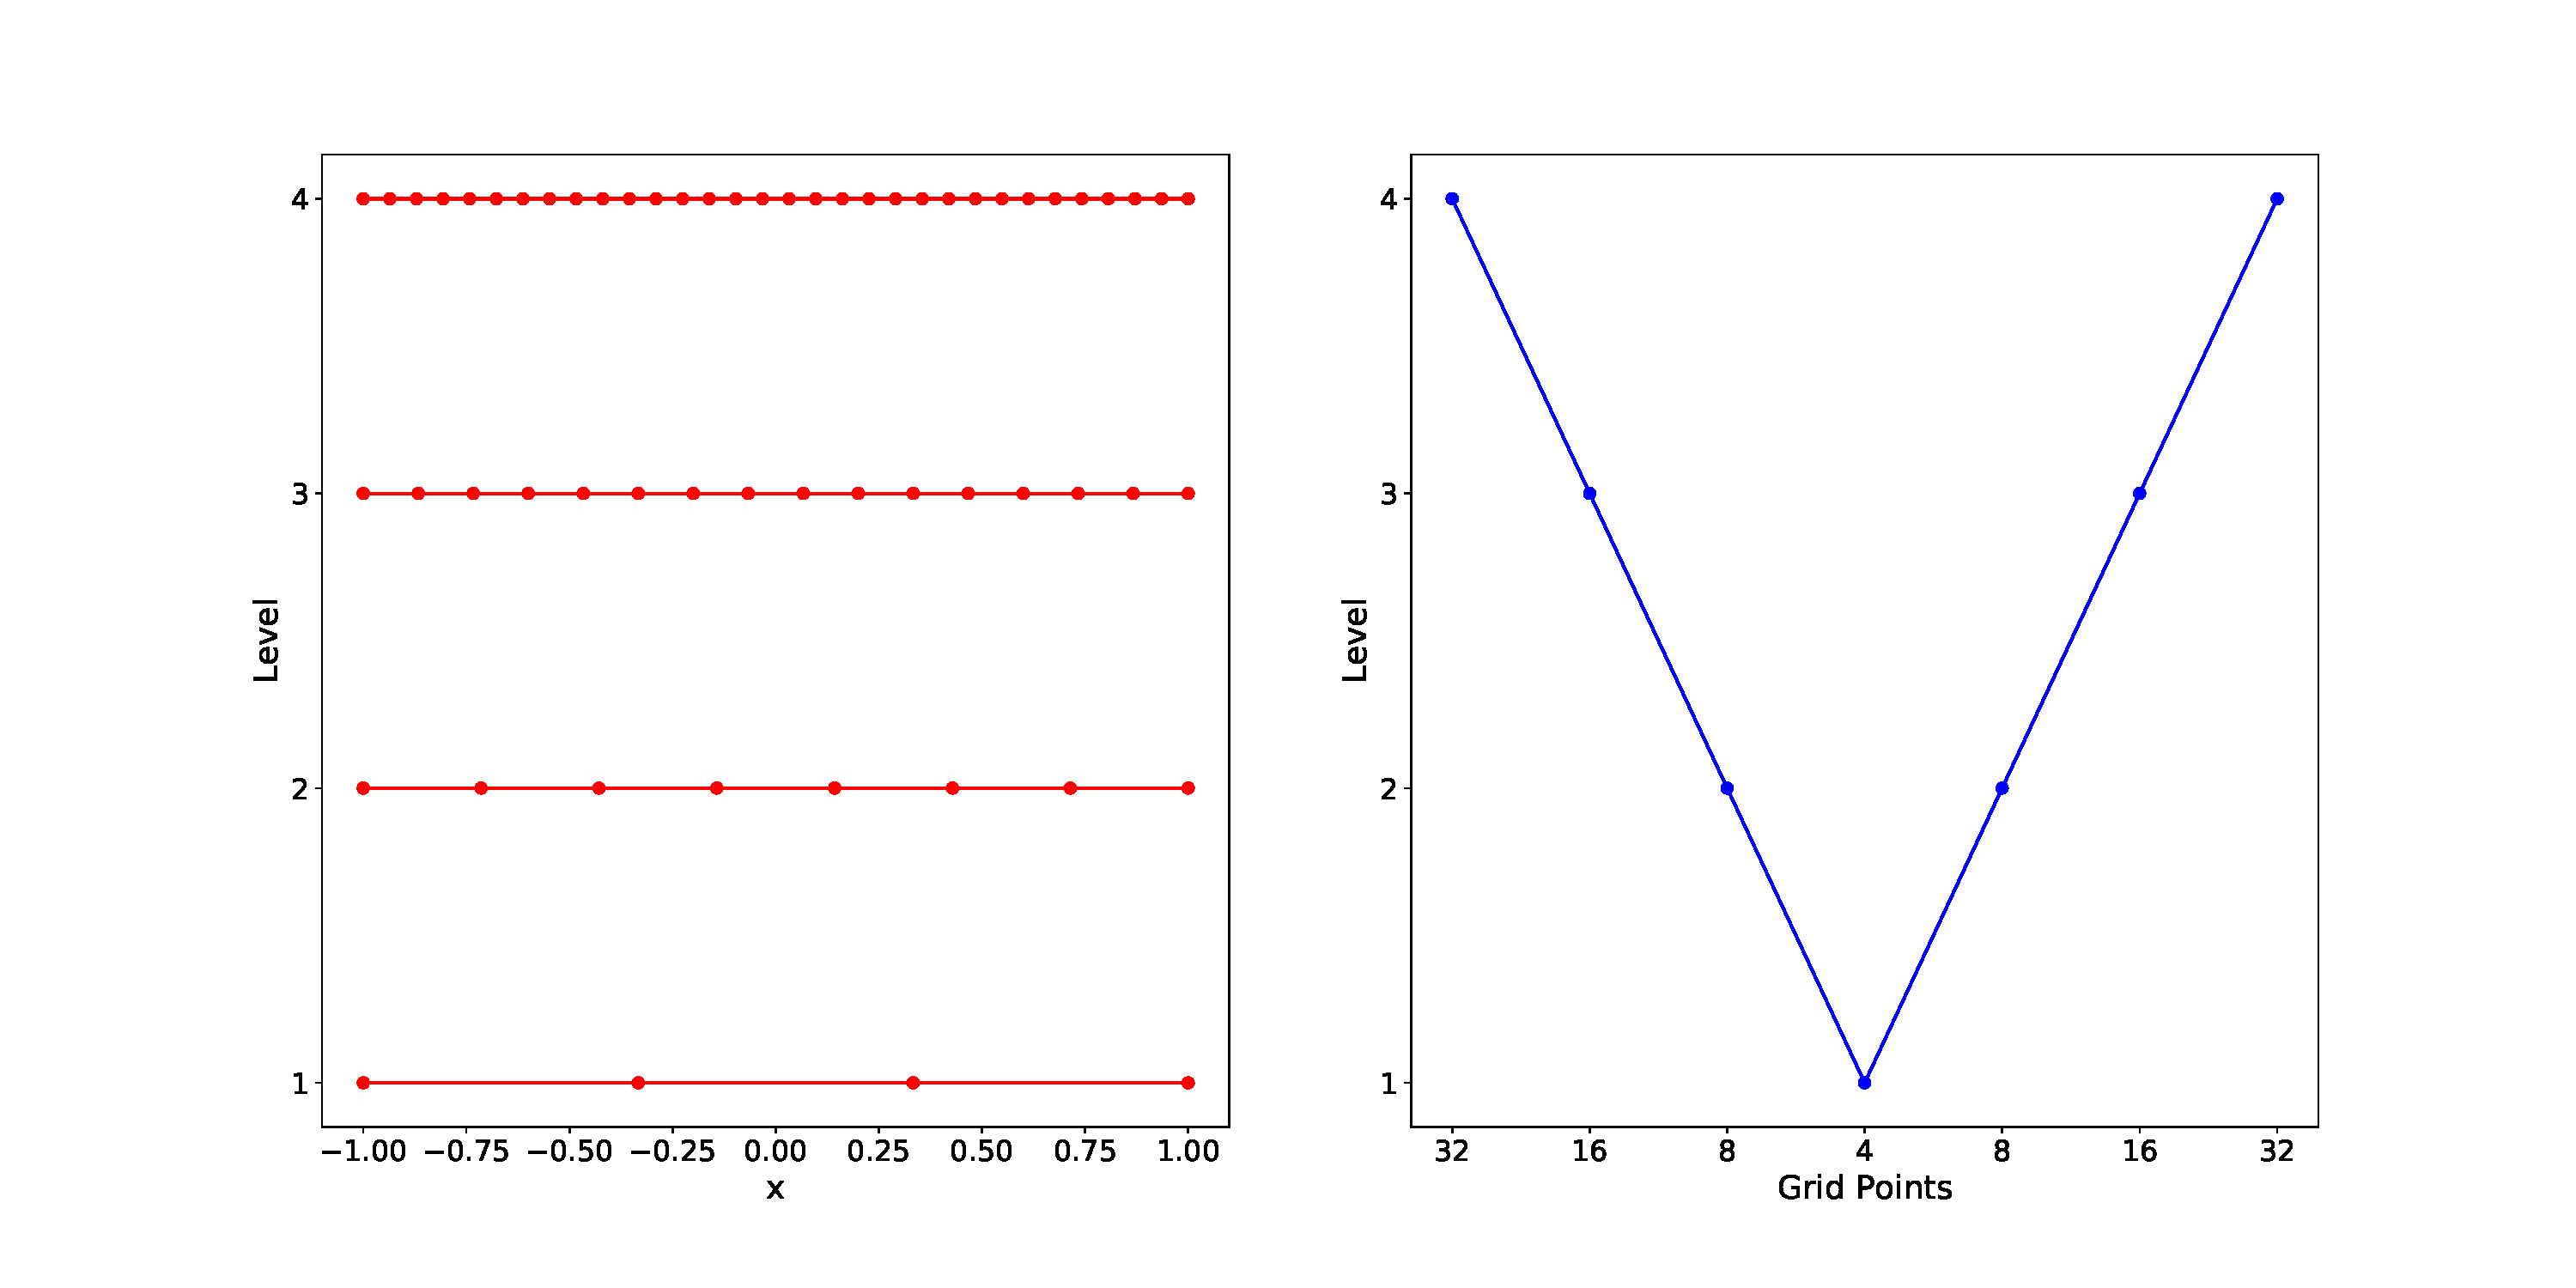
\includegraphics[width=0.8\columnwidth]{figures/multigrid.pdf}
    \caption{The 1D Multigrid Method. Starting with the finest grid, perform a few iterations of an iterative method. This is called relaxing the solution. Then project onto a coarser grid, and relax again. Repeat this down the levels in the grid to a desired precision. Once the solution is converged to on the coarsest level, interpolate back up the levels to obtain the solution on the finest level.}
    \label{fig:multigrid}
\end{figure}

In what is called the ``full multigrid" method, the process starts on the coarsest level instead of the finest. The solution is relaxed on this level, and then interpolated down onto a finer mesh. The interpolated solution is used as an initial guess for solving the problem on the finer mesh. The relaxed solution on a coarser grid is often an ideal initial guess for the problem on the finer mesh, resulting in quick convergence on that level.

The multigrid method allows one to accelerate an iterative solver. Multigrid methods are very effective as pre-conditioners for iterative methods. This is the general pattern of hierarchical methods: the ability to use classical iterative and direct methods on smaller grids where they perform well, and then ``scale" them up to larger problem sizes.

% \subsubsubsection{Nested Dissection}
% \label{subsub:nested-dissection}

{\bf Nested Dissection}
The nested dissection method formulated by \cite{george1973nested} is a direct method that builds upon Gaussian elimination for problems on a grid. It is the basis for the multifrontal method \citep{liu1992multifrontal, davis2004algorithm}. By taking advantage of the ordering of points on a grid, one can permute $\textbf{A}$ to first eliminate points that split the mesh into two disconnected meshes. This permutation takes the form of $\textbf{P}^* \textbf{A} \textbf{P}$, where the goal is to form $\textbf{P}$ to reorganize $\textbf{A}$ in a way that eliminates points in an efficient manner. This partitioning is then repeated until the entire mesh is partitioned into many disconnected meshes.

To detail nested dissection better, consider an $N \times N$ mesh such as a finite difference mesh discussed in Section \ref{subsub:finite-difference}. Assume that the initial ordering of points corresponds to an index set that iterates over the points in the mesh row-by-row. Now, the idea of nested dissection is to reorganize the points such that we first eliminate points down the middle of the mesh (i.e. the points at $x = 0$ in the first plot of Figure \ref{fig:discretization_methods}). Once these points are solved for, it splits the mesh into two equally sized pieces that are disconnected. Each of the disconnected meshes now are smaller, and thus easier to solve. This idea of splitting the mesh into disconnected pieces by first eliminating points along an interface can be recursively applied to each split. This means that after dividing the mesh into two, one can divide those two meshes into four meshes, and so on. Recursive splitting is a common characteristic in hierarchical methods.

Nested dissection was first introduced by \cite{george1973nested}, and further generalized by \cite{lipton1979generalized}. Martinsson provides a tutorial on nested dissection \citep{martinsson2019fast}. In fact, nested dissection served as motivation for another hierarchical method proposed by Martinsson and Gillman called the Hierarchical Poincaré-Steklov method.

% \subsubsubsection{The Hierarchical Poincaré-Steklov Method}
% \label{subsub:hps-method}

{\bf The Hierarchical Poincaré-Steklov Method}
Gillman and Martinsson introduce the Hierarchical Poincaré-Steklov (HPS) method \citep{martinsson2004fast, MARTINSSON2013460, gillman2014direct, martinsson2015hierarchical}. It is a direct solver for elliptic PDEs that is based on a binary tree of rectangular patches where the solution operator to $\textbf{A}$ is built by recursively merging child patches. Like direct methods, the HPS method involves a factorization step and a solve step. Unlike other direct methods, however, the HPS method is considered a matrix-free method as there is no requirement to form the system matrix $\textbf{A}$.

The HPS method starts with on a logically Cartesian domain, and recursively divides the domain in half. This creates a binary tree of patches as shown in Figure \ref{fig:solve}. Once the domain has been decomposed into this tree of patches, two operators are defined on the lowest level, called the leaf level. These operators are the solution operator $\textbf{S}$ and Dirichlet-to-Neumann (DtN) operator $\textbf{T}$. The solution operator maps boundary data to solution data on the interior of the patch (i.e. solves the local boundary value problem), and the DtN operator maps Dirichlet data on the boundary to Neumann data on the boundary. These operators can be formed using any elliptic PDE solver, including fast solvers like spectral methods. After forming these operators, the next step is to recursively merge each sibling patch up the tree. The merge step is demonstrated in Figure \ref{fig:merge}. This results in a global solution operator that can be stored and used multiple times. The final step is applying the solution operator to each level down the tree to obtain the solution everywhere in the domain. This is a series of matrix-vector multiplications.

Like other direct methods, the HPS method forms an in-memory solution operator that can be applied to several right-hand side vectors. This property makes it ideal for problems where several elliptic solves are necessary. While most iterative methods have better asymptotic performance than other direct methods, the HPS method can be accelerated using hierarchically block separable (HBS) matrix algebra to achieve near linear asymptotic performance \citep{gillman2014direct}.

The \gls{hps} method has been applied to solve 3D elliptic \gls{pdes} \citep{hao2016direct}, has been coupled with the spectral element method \citep{fortunato2020ultraspherical}, and implemented on adaptive meshes \citep{babb2018accelerated, geldermans2019adaptive,chipman2024fast}. Recently, the \gls{hps} method has also been implemented in parallel, targeting shared-memory machines \citep{beams2020parallel}, distributed-memory machines \citep{yesypenko2022parallel}, and \gls{gpu} devices \citep{yesypenko2022gpu}. More details on the \gls{hps} method can be found in Chapters 19--27 of \citep{martinsson2019fast} and a tutorial on the \gls{hps} method can be found in \citep{martinsson2015hierarchical}.

\begin{figure}
    \centering
    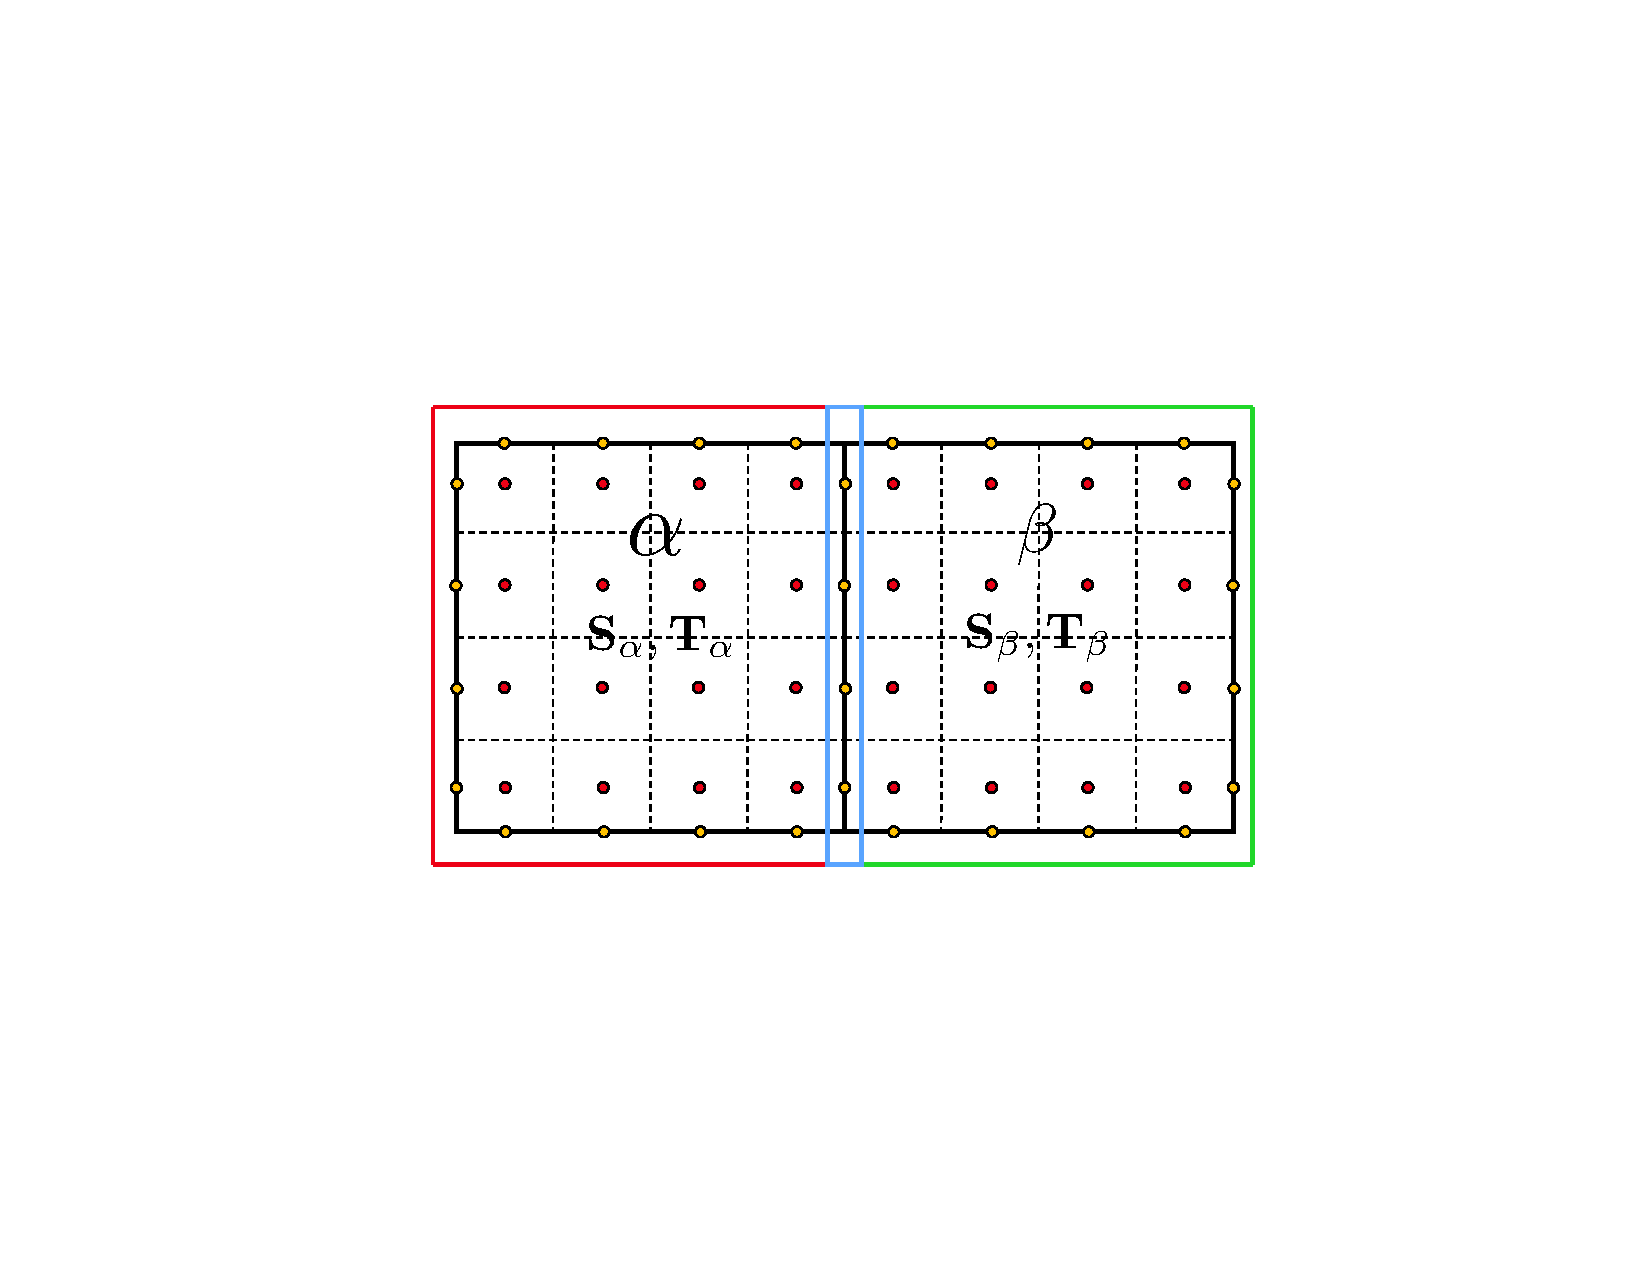
\includegraphics[width=0.7\columnwidth]{figures/merge_figure.pdf}
    \caption{HPS Merge Operation. The merged patch $\Omega_{\tau}$ is the union of children $\Omega_{\alpha}$ and $\Omega_{\beta}$, i.e. $\Omega_{\tau} = \Omega_{\alpha} \cup \Omega_{\beta}$. Red, green, and blue nodes correspond to index sets $\textbf{I}_1$, $\textbf{I}_2$, and $\textbf{I}_3$, respectively. The merge operation eliminates the nodes on the interface of the children patches.}
    \label{fig:merge}
\end{figure}

\begin{figure}
    \centering
    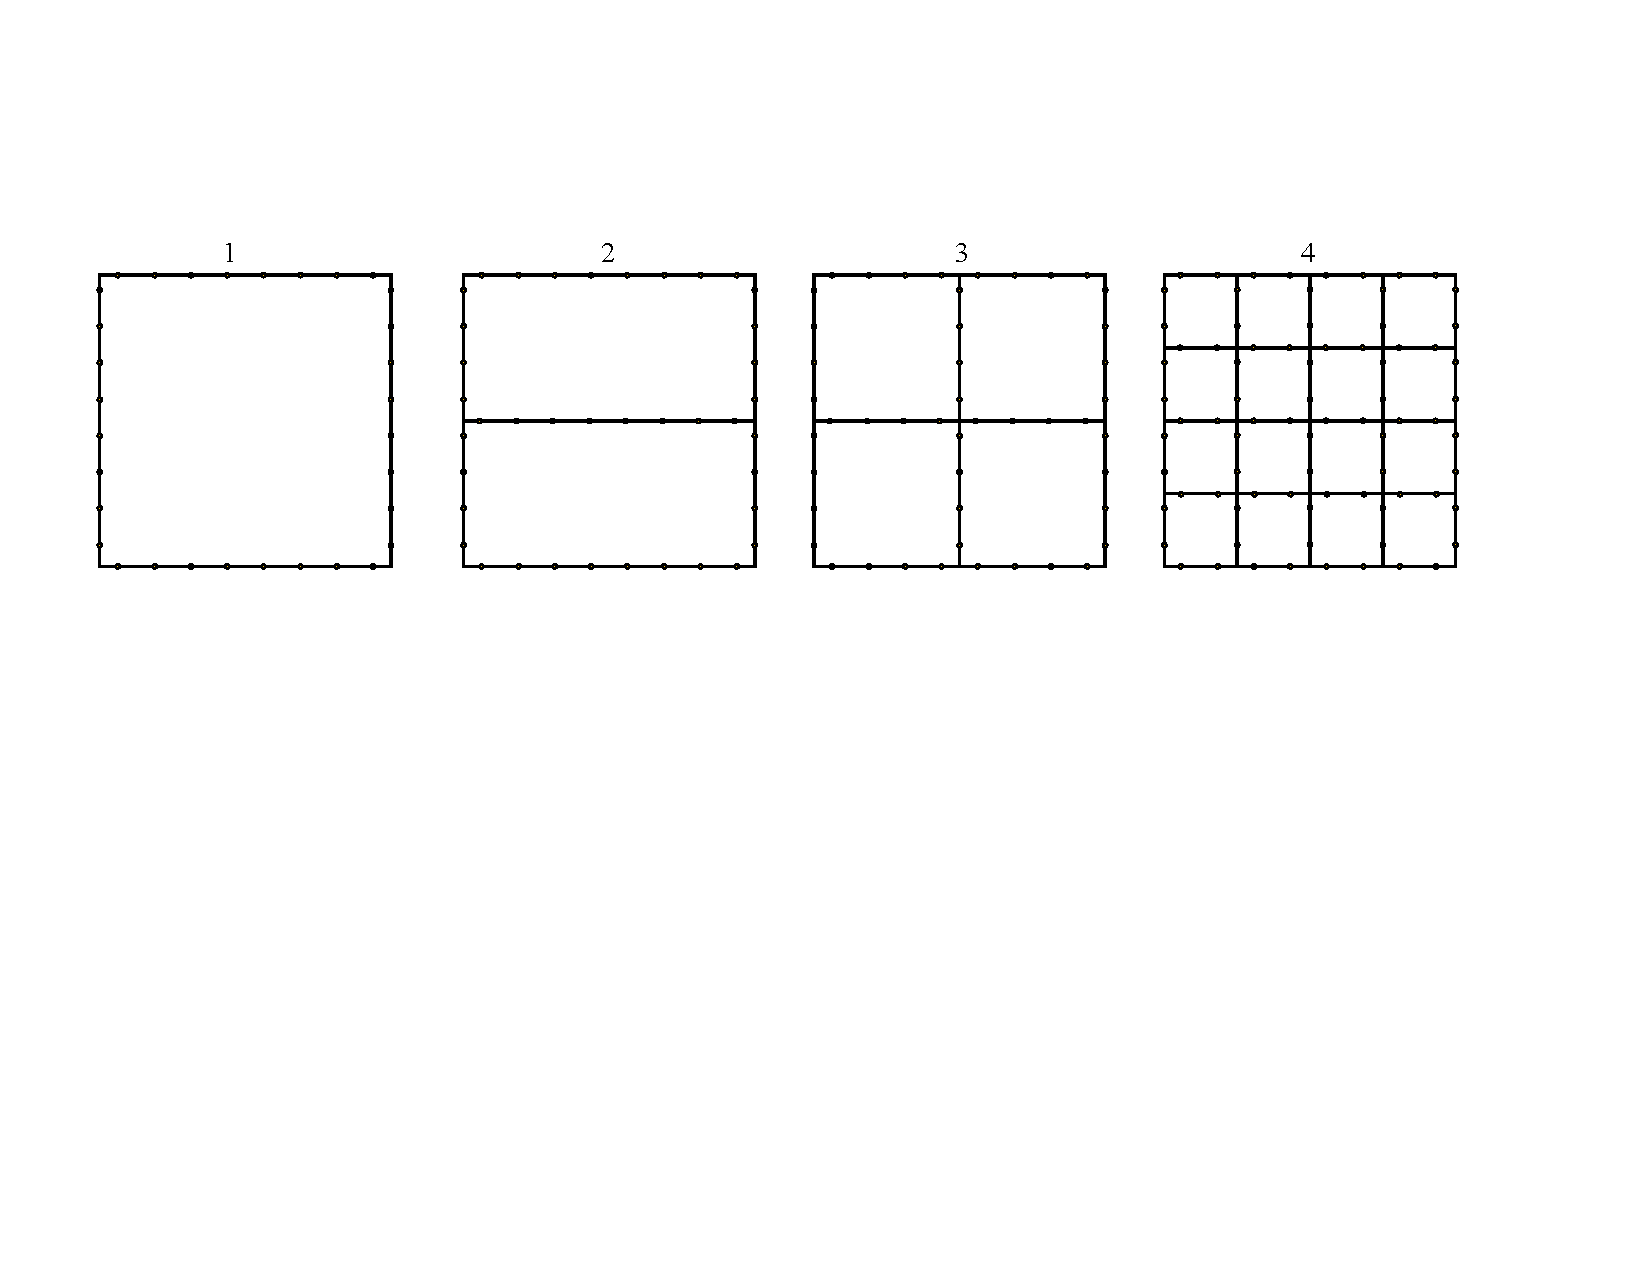
\includegraphics[width=\columnwidth]{figures/solve_figure.pdf}
    \caption{HPS Solve Stage. Once $\textbf{S}_0$ is formed, apply it to the top level Dirichlet data to get boundary (and solution) data on the interface of the children. Apply the patch solution operator down the tree until each leaf has its local boundary information. Then apply the solution operator to get the solution data in the interior of each leaf.}
    \label{fig:solve}
\end{figure}


% \subsection{Fast Solvers for Elliptic PDEs}

% The linear systems formed by discretizations of elliptic \gls{pdes} are sparse and banded. Numerical linear algebra techniques that take advantage of this structure are ideal. Efficient solvers have been developed for uniform Cartesian meshes, such as the Unsymmetrical Multifrontal method implemented in the UMFPACK code \citep{davis2004algorithm} or the Cyclic Reduction method \citep{swarztrauber1974direct} as implemented in the FISHPACK library \citep{swarztrauber1999fishpack,adams2016fishpack90}.

% \citet{gillman2014direct} describe a direct solver for elliptic problems on a binary tree structure. The goal is to build up a factorization by successively merging subdomains via a class of Poincar\'e-Steklov operators \citep{quarteroni1991theory} called \gls{d2n} operators. It is a domain decomposition method that was originally inspired by the partitioning scheme of nested dissection \citep{george1973nested,lipton1979generalized}. This approach does not require any matrix assembly on the composite mesh and can be used with any uniform grid solver at the leaf level. In their original work, \citet{gillman2014direct} use high-order spectral collocation methods and low-rank optimization to achieve $\mathcal O(N)$ factorization complexity. This method has come to be known as the \gls{hps} method \citep{martinsson2015hierarchical}. The \gls{hps} method has been applied to solve 3D elliptic \gls{pdes} \citep{hao2016direct}, has been coupled with the spectral element method \citep{fortunato2020ultraspherical}, and implemented on adaptive meshes \citep{babb2018accelerated, geldermans2019adaptive,chipman2024fast}. Recently, the \gls{hps} method has also been implemented in parallel, targeting shared-memory machines \citep{beams2020parallel}, distributed-memory machines \citep{yesypenko2022parallel}, and \gls{gpu} devices \citep{yesypenko2022gpu}. More details on the \gls{hps} method can be found in Chapters 19--27 of \citep{martinsson2019fast} and a tutorial on the \gls{hps} method can be found in \citep{martinsson2015hierarchical}. A more in-depth description of the \gls{hps} method outlined by \citet{gillman2014direct} will be provided in \refsec{subsub:hps-method}.

% \damyn{[Direct vs. iterative solvers discussion.]}

\subsection{Parallelism and Software}

Parallel linear solvers using iterative or direct methods have been successfully developed and implemented. Parallel iterative methods include GMRES \citep{saad1986gmres}, the conjugate gradient method \citep{hestenes1952methods}, the \gls{amg} method \citep{yang2002boomeramg}, and the \gls{gmg} method \citep{sundar2012parallel} (with a good overview provided by \citet{chow2006survey}). Parallel direct methods include matrix factorization methods like LU-factorization, Cholesky factorization and the spectral value decomposition \citep{donfack2015survey, demmel1999asynchronous, gupta1997highly}.

% References for parallel methods?

Several, large-scale and open-source codes currently exist to solve linear systems formed from elliptic PDEs. The hypre library \citep{falgout2002hypre} features scalable preconditioners for parallel multigrid methods. The SuperLU library \citep{li2005superlu} is a general purpose library for solving sparse linear systems using direct methods. Additional codes like PETSc \citep{anl2023petsc}, FLASH-X \citep{dubey2022flash}, and AMReX \citep{zhang2019amrex}, contain iterative and direct solvers that also work with \gls{amr}. The ForestClaw code \citep{calhoun2017forestclaw} coupled with the ThunderEgg repository \citep{aiton2022thunderegg} implements hyperbolic and elliptic solvers for finite volume meshes on adaptively refined quadtrees and octrees provided from \pforest. \pforest\ \citep{burstedde2011p4est,burstedde2020parallel} is a highly scalable AMR code that provides quadtree and octree data structures for users to build on top of. The EllipticForest library \citep{chipman2024ellipticforest} contains an implementation of the quadtree-adaptive HPS method, including the parallel algorithms outlined in this paper. Another code of interest is the ButterflyPACK library \citep{liu2018butterflypack} which solves large-scale dense systems with off-diagonal, low-rank structure like the matrices formed in the HPS method.
\section{Novelty of this Work}

The work presented in this dissertation is novel and broadens the field of fast, adaptive, and direct solvers for elliptic PDEs. Largely based on the HPS method of Gillman and Martinsson in \cite{gillman2014direct,martinsson2019fast} and focused on application with codes like \pforest\ \cite{burstedde2011p4est,burstedde2020parallel} and ForestClaw \cite{calhoun2017forestclaw}, this research includes significant contributions to the current literature. Modifying the HPS method for use with quadtree mesh data structures and on finite volume patches, the quadtree-adaptive HPS method that is outlined in \refchap{chap:qahps} and \refchap{chap:adaptive-build} is novel. The parallel implementation outlined in \refchap{chap:parallel} is also novel compared to current shared memory implementations.

The research presented herein has been highlighted in peer-reviewed journals. \damyn{Add more here; JOSS, JCP, and (potentially) others.}
\section{Overview}

This document will continue as follows:

\begin{itemize}
    \item asdf
    \item asdf
    \item asdf
\end{itemize}

% \chapter{Elliptic PDEs and Classic Solution Methods}
% \label{chap:elliptic-pdes}
% \section{The Elliptic Partial Differential Equation}
\label{sec:the-elliptic-pde}

Partial differential equations are classified by their highest order derivative terms. A second order, linear differential equation can be written as
\begin{align*}
    A(\textbf{x}) \frac{\partial^2 u(\textbf{x})}{\partial x^2} + B(\textbf{x}) \frac{\partial^2 u(\textbf{x})}{\partial x \partial y} + C(\textbf{x}) \frac{\partial^2 u(\textbf{x})}{\partial y^2} + ... \\
    ... + D(\textbf{x}) \frac{\partial u(\textbf{x})}{\partial x} + E(\textbf{x}) \frac{\partial u(\textbf{x})}{\partial y} + F(\textbf{x}) u(\textbf{x}) + G(\textbf{x}) &= 0.
\end{align*}
Second-order linear PDEs are classified according to the value of the determinant of this expression:
\begin{align*}
    B^2 - 4AC &< 0,\ \ \ \text{Elliptic} \\
    B^2 - 4AC &= 0,\ \ \ \text{Parabolic} \\
    B^2 - 4AC &> 0,\ \ \ \text{Hyperbolic}
\end{align*}

In this overview, we will consider common elliptic PDEs such as the Poisson equation
\begin{align}
    \nabla \cdot \left( \beta(\textbf{x}) \nabla u(\textbf{x}) \right) &= f(\textbf{x}),
    \label{eq:variable_poisson}
\end{align}
and the Helmholtz equation
\begin{align}
    \nabla \cdot \left( \beta(\textbf{x}) \nabla u(\textbf{x}) \right) + \lambda(\textbf{x}) u(\textbf{x}) &= f(\textbf{x}),
    \label{eq:variable_helmholtz}
\end{align}
where $\textbf{x} = [x, y]$, $\nabla = (\frac{\partial}{\partial x}, \frac{\partial}{\partial y})$, $\nabla^2 = \nabla \cdot \nabla = \frac{\partial^2}{\partial x^2} + \frac{\partial^2}{\partial y^2}$, and $\textbf{x} \in \Omega \subset \mathcal{R}^2$. When $\beta(\textbf{x}) = 0$ and $\lambda(\textbf{x}) = \kappa^2$ ($\kappa$ is a constant), these expressions reduce to the more classical, constant coefficient versions of the Poisson and Helmholtz equations. When the right-hand side function $f(\textbf{x}) = 0$, these are homogeneous problems, where \refeq{eq:variable_poisson} is reduced to the Laplace equation. Each of these PDEs are subject to the appropriate boundary conditions on the domain boundary $\partial \Omega = \Gamma$. Such boundary conditions (BCs) can either be Dirichlet (Type-I), Neumann (Type-II), or Robin/Mixed (Type-III) BCs. Dirichlet problems impose the value of $u$ on the boundaries, Neumann problems impose the flux or normal gradient $\partial_n u$ on the boundaries, while Robin problems impose a linear combination of Dirichlet and Neumann type BCs.

Although analytical solutions exist for some simple variations of the problems above, we are interested in looking at numerical methods to solve these equations. To do so, we look at various ways to discretize the domain $\Omega$. This discretization will lead to a linear system of equations which we will solve with numerical methods, taking advantage of the sparsity and structure of the associated system.
% \section{Numerical Methods for Elliptic PDEs}
\label{sec:numerical-methods-for-elliptic-pdes}

\subsection{Finite Difference}

\begin{figure}
    \centering
    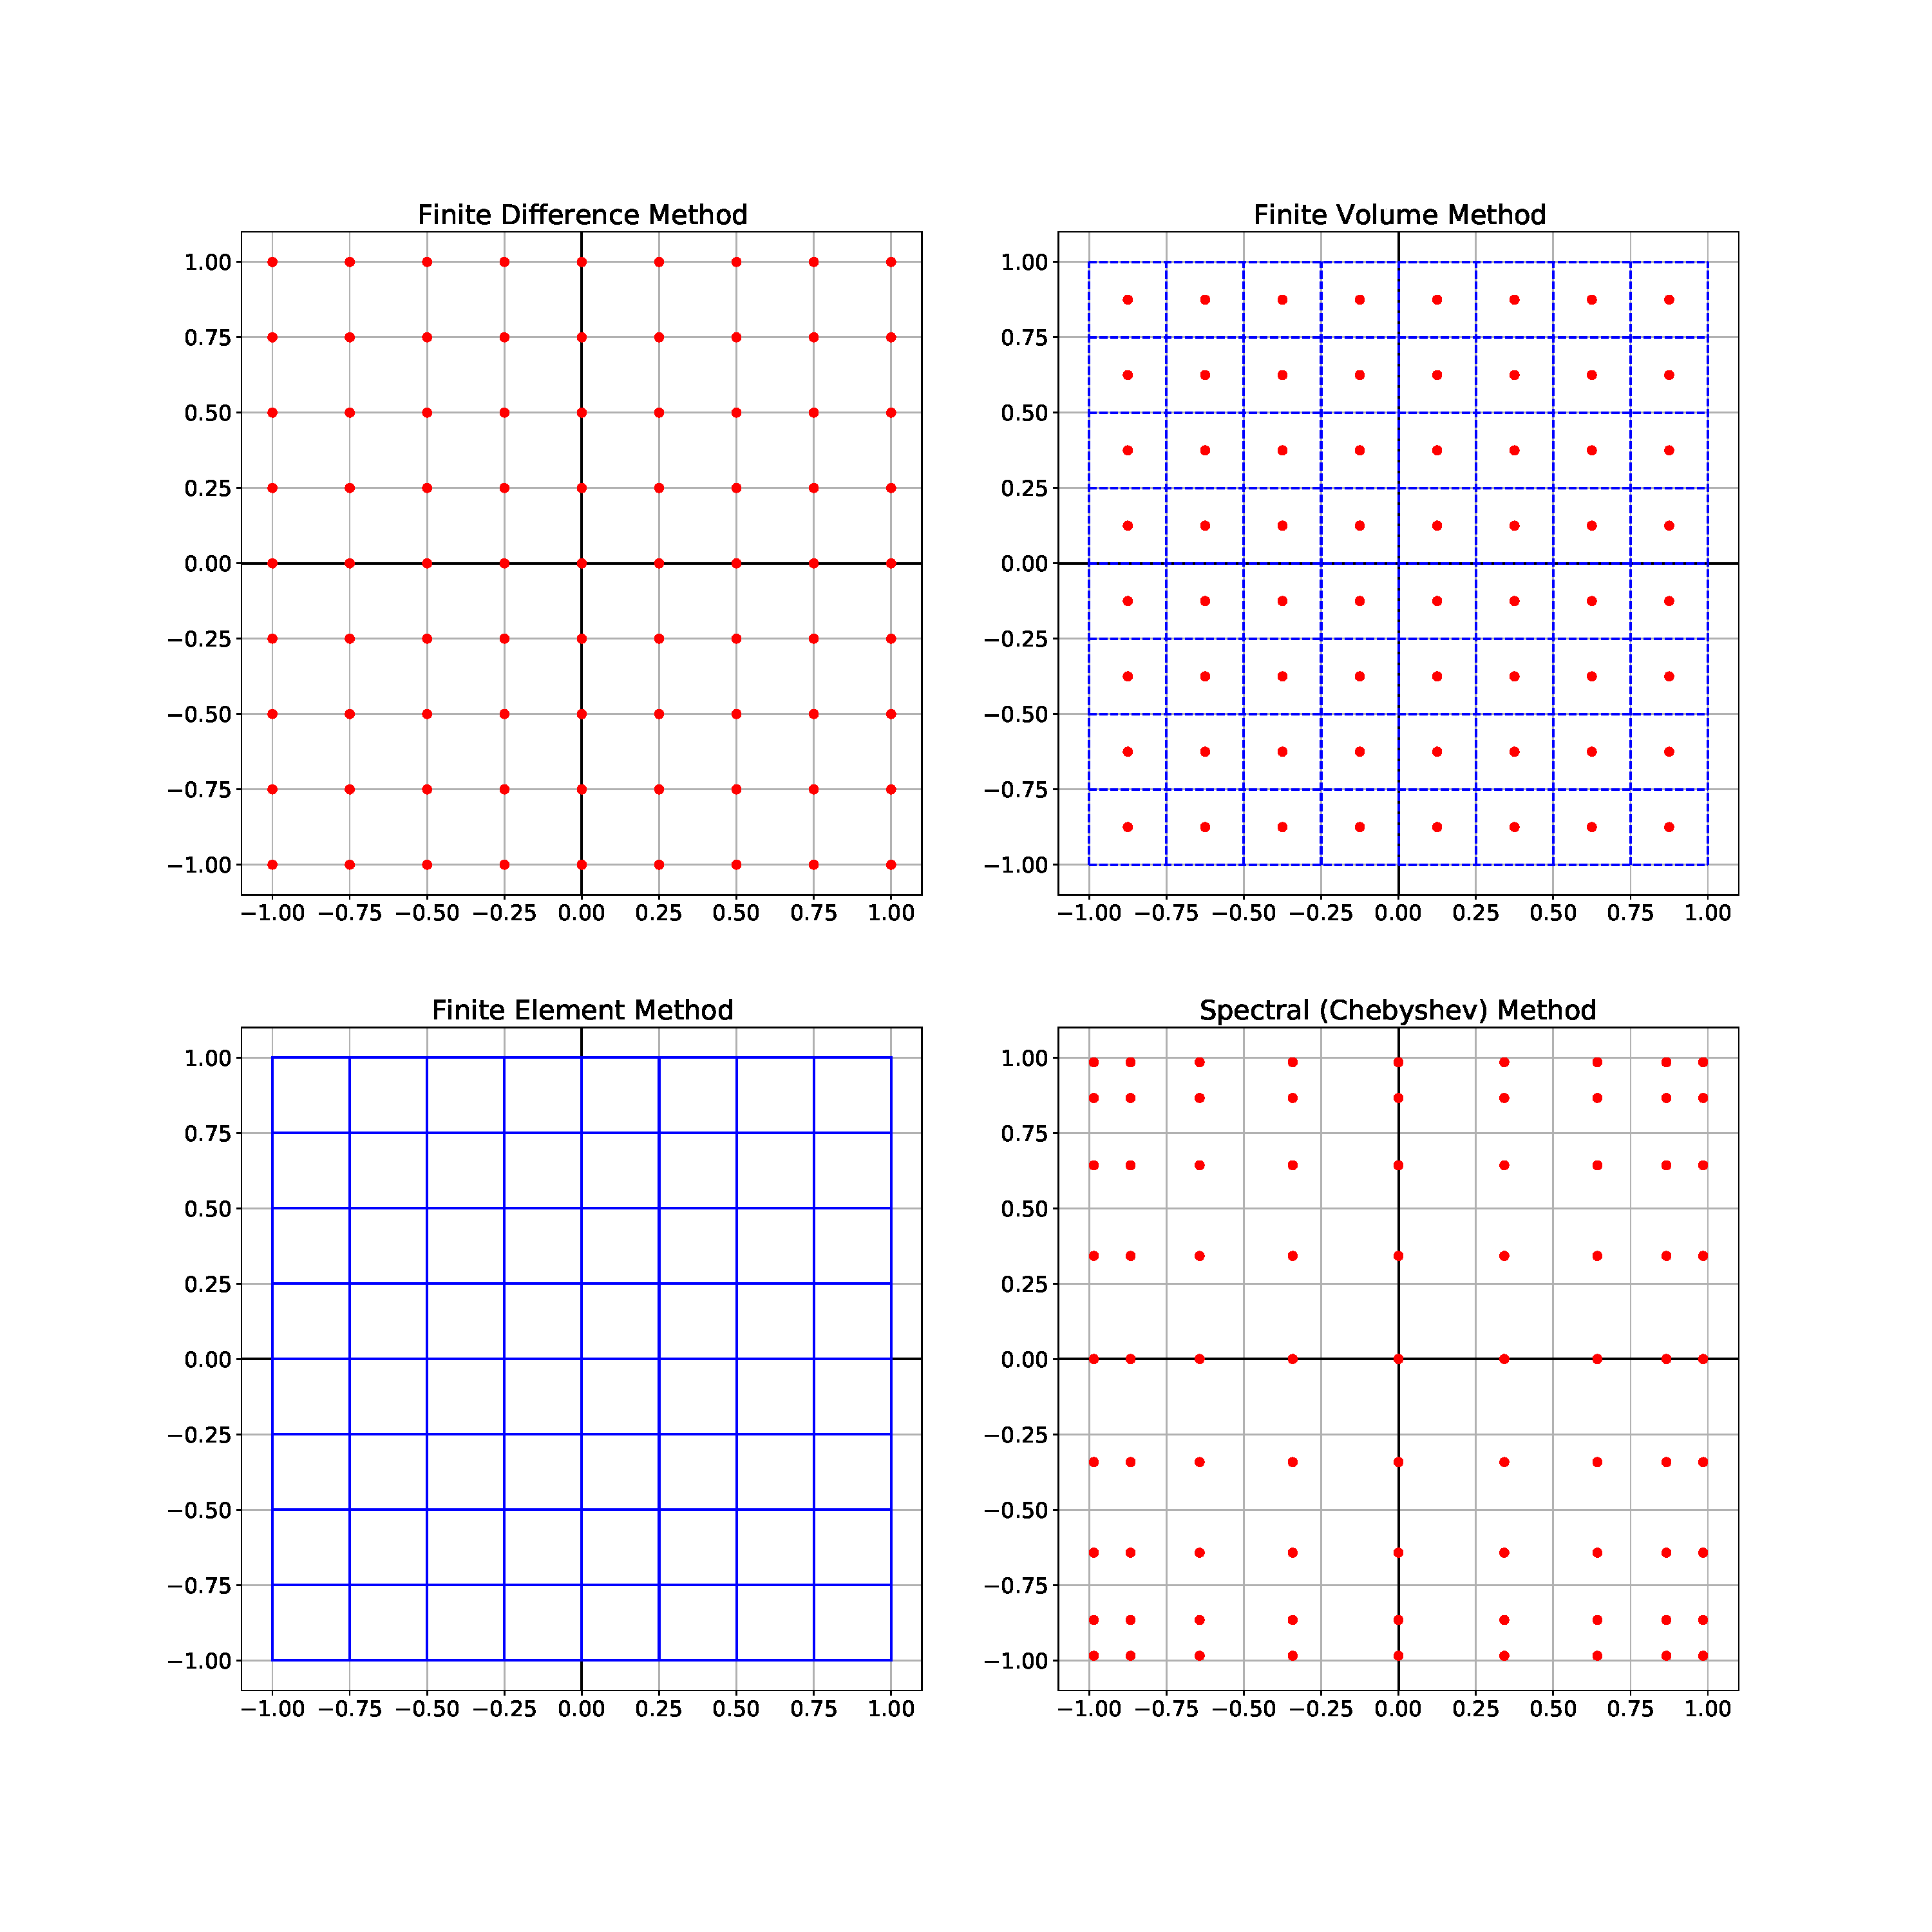
\includegraphics[width=0.8\columnwidth]{figures/PDE_discretization_methods.pdf}
    \caption{Discretization Methods. Top Left: Finite difference grid based on a mesh of points or nodes. Top Right: Finite volume mesh made of cells (dashed blue boxes) with cell averages in the center (red points). Bottom Left: Finite element mesh where each blue box is an element with a shape function defined at all points within the element. Bottom Right: Spectral mesh made up of a tensor of Chebyshev nodes.}
    \label{fig:discretization_methods}
\end{figure}

If $\Omega$ is on a logically rectangular domain (i.e. 2D Cartesian plane), perhaps the simplest discretization of the domain $\Omega$ is by collocating a mesh of points throughout the domain. Given upper and lower bounds in both directions, $[x_l, x_u], [y_l, y_u]$, the x- and y-location of each point can be defined as
\begin{align}
    x_i &= x_l + i \Delta x,\ \ \ i = 0, 1, ..., N_x-1 \\
    y_i &= y_l + j \Delta y,\ \ \ j = 0, 1, ..., N_y-1
\end{align}
where $N_x, N_y$ is the number of points in the x- and y-direction and grid spacing is defined as
\begin{align}
    \Delta x &= \frac{x_u - x_l}{N_x - 1} \\
    \Delta y &= \frac{y_u - y_l}{N_y - 1}.
\end{align}
These points are shown in the first plot of Figure \ref{fig:discretization_methods}. This type of discretization is known as the {\em finite difference method}. \damyn{(Cite something here?)}. In the finite difference approach, the expressions for the derivatives in a PDE are replaced with Taylor series approximations. For example, a second order accurate, central-difference approximation to the second derivative can be given as
\begin{align}
    \frac{\partial^2 u}{\partial x^2} &= \frac{u(x - \Delta x, y) - 2u(x, y) + u(x + \Delta x, y)}{\Delta x^2} + \mathcal{O}(\Delta x^2)
\end{align}
and if we let $u(x_i, y_j) = u_{i,j}$, then we can write this as
\begin{align}
    \frac{\partial^2 u}{\partial x^2} &= \frac{u_{i-1,j} - 2u_{i,j} + u_{i+1,j}}{\Delta x^2} + \mathcal{O}(\Delta x^2).
\end{align}
Using these Taylor Series expansions, we can replace the continuous Poisson's equation \ref{eq:variable_poisson} with the discrete system of equations:
\begin{align}
    \frac{u_{i-1,j} - 2u_{i,j} + u_{i+1,j}}{\Delta x^2} + \frac{u_{i,j-1} - 2u_{i,j} + u_{i,j+1}}{\Delta y^2} &= f_{i,j}.
    \label{eq:poisson_FD}
\end{align}
For each grid point $i = 0, ..., N_x - 1$, $j = 0, ..., N_y - 1$ this expression forms a linear system with $(N_x-1) \times (N_y-1)$ unknowns.

The system that is formed from this discretization is sparse and banded. For example, let $N_x = N_y = N$ for simplicity (thus $\Delta x = \Delta y = h$). Index the vector $\textbf{u}$ first by rows, then by columns, such that
\begin{align}
    \textbf{u} = [u_{0,0}, ..., u_{N - 1, 0}, u_{0, 1}, ..., u_{N - 1, 1}, ..., u_{0, N - 1}, ..., u_{N - 1, N - 1}]^T.
\end{align}
The corresponding linear system from \ref{eq:poisson_FD} is the following:
\begin{align}
    \textbf{A} &= \frac{1}{h^2}
    \begin{bmatrix}
        \textbf{D} & \textbf{I}_{N} & \textbf{0} & ... & \textbf{0} \\
        \textbf{I}_{N} & \textbf{D} & \textbf{I}_{N} & ... & \textbf{0} \\
        \textbf{0} & \textbf{I}_{N} & \textbf{D} & ... & \textbf{0} \\
        \vdots & \vdots & \vdots & \ddots & \vdots \\
        \textbf{0} & \textbf{0} & \textbf{0} & ... & \textbf{D}
    \end{bmatrix}
\end{align}
where
\begin{align}
    \textbf{D} &= 
    \begin{bmatrix}
        -4 & 1 & 0 & ... & 0 \\
        1 & -4 & 1 & ... & 0 \\
        0 & 1 & -4 & ... & 0 \\
        \vdots & \vdots & \vdots & \ddots & \vdots \\
        0 & 0 & 0 & ... & -4
    \end{bmatrix}.
\end{align}
We also index the RHS similarly to $u(x,y)$ resulting in a RHS vector $\textbf{f}$. This leads to the linear system
\begin{align}
    \textbf{A} \textbf{u} = \textbf{f} + \textbf{b}
\end{align}
where $\textbf{b}$ contains any updates necessary for any type of boundary condition.

\subsection{Finite Volume}

In a finite volume scheme, the domain is broken up into cells, which can be structured or unstructured polygons (2D) or polyhedrons (3D). The function to approximate is solved for in terms of a cell average. Finite volume schemes are often used to solve equations modeling conservation laws, where the cell quantity is conserved in time through balancing fluxes (what comes in and out of the cell boundaries) and the cell source (what the cell is generating or destroying). In a finite volume scheme, the cell average is updated according to the integral formulation of the conservation law as
\begin{align}
    \frac{\partial}{\partial t} \int_{\Omega_i} \textbf{q} d\Omega_i + \int_{\Gamma_i} \textbf{F}(\textbf{q}) \cdot \hat{n}_i d\Gamma_i + \int_{\Omega_i} \textbf{s} d\Omega_i = 0,
\end{align}
where $\Omega_i$ and $\Gamma_i$ are the cell domains and boundaries, respectively, $\textbf{q}$ is a vector of quantities in each cell, $\textbf{F}$ is a flux function, and $\textbf{s}$ is the cell's source term. In the second plot of Figure \ref{fig:discretization_methods}, the blue dashed lines are the cell boundaries, and the red points are the cell centers. For up to second order schemes, the cell average is collocated at the center of the cell; this changes for higher order schemes.

\subsection{Finite Element}

In a finite element scheme, the domain is broken into elements. These elements can also be structured or unstructured polygons (2D) or polyhedrons (3D), similar to the finite volume method. The PDE to solve is converted into a weak form by multiplying the PDE by a test function $v(x,y)$ and integrating over the domain:
\begin{align}
    \int_{\Omega} v \nabla^2 u d\Omega &= \int_{\Omega} vf d\Omega.
\end{align}
Green's Theorem (i.e., integration by parts) is used to break the LHS into integrals on the domain $\Omega$ and the boundary $\partial \Omega = \Gamma$:
\begin{align}
    -\int_{\Omega} \nabla v \cdot \nabla u d\Omega + \int_{\Gamma} v \frac{\partial u}{\partial n} d\Gamma &= \int_{\Omega} vf d\Omega
    \label{eq:poisson_weak_form}
\end{align}
The idea behind the finite element method is to use basis functions
\begin{align}
    u(x,y) \approx \bar{u} = \sum_{k=1}^{N_k} c_k \phi(x,y)
\end{align}
inside each element $\Omega_i$, where $\Omega = \cup_{i = 1}^{N_{\text{elem}}} \Omega_i$. When the same basis functions for the test functions $v$ are also used, this leads to the Galerkin finite element method. Upon substitution of the above into \ref{eq:poisson_weak_form}, and integrating the basis function with either quadrature or with analytical expressions, a linear system is formed for the coefficients $c_k$.

There are several variations of the finite element method. The method explained above forms a global linear system involving all elements. To avoid this, mapping a physical element to some reference element, makes the contributions from a single element only influence itself and its neighbors. This makes the coefficient matrix in the linear system much more sparse and structured, making it easier to solve. Additionally, by not imposing continuity across element boundaries, one arrives at the discontinuous Galerkin method, where the discontinuities are handled through element fluxes. By choosing certain shape or basis functions, one can derive different variations of the finite element method, including the B-spline finite element method \cite{kagan1998new} and the spectral element method \cite{patera1984spectral}.

\subsection{Spectral Methods}

In spectral methods, the approach is to approximate the solution $u$ as a linear combination of a finite set of orthogonal basis functions
\begin{align}
    u(x,y) = \sum_{i=1}^{N_x} \sum_{j=1}^{N_y} c_{i,j} \phi_{i}(x) \phi_{j}(y)
\end{align}
where the coefficients are chosen to minimize a norm, such as the $L^2$ norm of the residual $r(x,y) = \nabla^2 u(x,y) - f(x,y)$. On a discrete domain, this is similar to requiring $\nabla^2 u(x_i, y_j) = f(x_i, y_j)$ at all interior grid points. As this acts like an interpolation scheme, increasing the number of discretization points on with a fixed interval actually leads to highly oscillatory results. Thus, in spectral methods, it is common to use grid points that are clustered near the ends of the interval, such as Chebyshev points, defined on an interval $[a,b]$ as
\begin{align}
    x_i &= a + \frac{1}{2}(b - a)\Big(1 + \cos \big( \pi (1 - \frac{i}{N + 1}) \big) \Big), i = 0, ..., N + 1.
\end{align}
These points are shown on the last plot of Figure \ref{fig:discretization_methods}. With a good basis of grid points, spectral methods can achieve very fast convergence. The linear system formed by this method will be dense as it functions like a high-order interpolation scheme. However, as convergence is much faster than high-order finite difference methods, one can use far fewer points on a grid, so the size of the system is kept small. If one uses Fourier series as the basis functions $\phi$, one can accelerate the solution of the linear system using fast Fourier Transform algorithms. Though, due to the periodic nature of the Fourier series, it is more difficult to implement non-periodic boundary conditions (\cite{leveque2007finite}, \cite{townsend2015automatic}).

% [TODO: Rework this section]
%
% In each of the methods presented above, the function approximation is found by forming and solving a linear system. In spectral methods, one uses integral transformations such as the Fourier or Laplace Transforms to differentiate. For example, the Fourier Transform of a function is given as
% \begin{align}
%     F(k) = \mathcal{F}[f(x)] = \frac{1}{\sqrt{2\pi}} \int_{-\infty}^{\infty} f(x) e^{ikx} dx
% \end{align}
% with it's inverse
% \begin{align}
%     f(x) = \mathcal{F}^{-1}[F(k)] = \frac{1}{\sqrt{2\pi}} \int_{-\infty}^{\infty} F(k) e^{ikx} dk.
% \end{align}
% The strength of these methods show when considering the derivatives of $f(x)$:
% \begin{align}
%     \frac{\partial^n f}{\partial x^n} &= \frac{\partial^n}{\partial x^n} \frac{1}{\sqrt{2\pi}} \int_{-\infty}^{\infty} F(k) e^{ikx} dk \\
%     &= \frac{1}{\sqrt{2\pi}} \int_{-\infty}^{\infty} (ik)^{n} F(k) e^{ikx} dk
% \end{align}
% So any $nth$ derivative can be expressed in terms of a Fourier and inverse Fourier transform:
% \begin{align}
%     \frac{\partial^n f}{\partial x^n} &= \mathcal{F}^{-1}[(ik)^n \mathcal{F}[f(x)]].
% \end{align}
% In practice, one can use fast algorithms such as the famous Fast Fourier Transform to perform this arithmetic.
%
% A minor drawback to this method is the need to work on a periodic domain in order for the Fourier Transform to function properly. This makes enforcing boundary conditions difficult. Thus, extensions to spectral methods include using a better basis of points than evenly spaced points, such as Chebyshev nodes. Chebyshev nodes defined in the interval $(-1, 1)$ are given as
% \begin{align}
%     x_k = \cos \Big( \frac{2k - 1}{2n} \pi \Big), k = 1, ..., n.
% \end{align}
% Using these nodes can increase the accurarcy of the method as well as provide a better set of collocation points for interpolation \cite{igel1999wave}.

\subsection{Other Methods and Summary}

These methods are not all the possible ways to solve an elliptic PDE. Other methods include using quadrature methods on the integral formulation of the PDE, as well as collocation methods such as radial basis function approximations. However, the methods we reviewed show some of the most classic approaches to solving elliptic PDEs.

% \section{Solution Methods for Elliptic Partial Differential Equations}
\label{sec:solution-methods-for-elliptic-pdes}

The discretization methods described in \refsec{sec:numerical-methods-for-elliptic-pdes} result in a linear system. To generally talk about these solution methods, we assume that we form the linear system
\begin{align}
    \textbf{A} \textbf{u} = \textbf{b}
    \label{eq:ls}
\end{align}
where $\textbf{A} \in \mathbb{R}^{N \times N}$ is a coefficient matrix formed from one of the discretization methods, $N$ is the number of degrees of freedom, $\textbf{u} = u_i = u(x_i)$ for $i \in \textbf{I}_x$, index set $\textbf{I}_x$ for the discrete domain, and $\textbf{b}$ is the right-hand side vector encoded with the boundary conditions and the inhomogeneous function $f(\textbf{x})$. The goal is to solve for $\textbf{u}$ where we take advantage of the sparsity and structure of $\textbf{A}$. We organize the various methods into the following three categories: 1) iterative methods, 2) direct methods, and 3) hierarchical methods.

\subsection{Iterative Methods}
\label{sub:iterative-methods}

Iterative methods start with an initial guess of a solution to \ref{eq:ls} and correct the iterate until convergence to a specified tolerance. The simplest iterative methods are called splitting methods where the linear system is modified according to
\begin{align}
\textbf{A} = \textbf{M} - \textbf{N} \Rightarrow \textbf{M} \textbf{u} = \textbf{N} \textbf{u} + \textbf{b}.
\end{align}
This suggests the following recursion relationship for the next iteration:
\begin{align}
\textbf{M} \textbf{u}^{k+1} &= \textbf{N} \textbf{u}^k + \textbf{b} \\
\textbf{u}^{k+1} &= \textbf{M}^{-1} \textbf{N} \textbf{u}^k + \textbf{M}^{-1} \textbf{b}.
\end{align}
The idea is to choose $\textbf{M}$ that captures as much of $\textbf{A}$ as possible, but is still easy and quick to invert. As $\textbf{A}$ is either banded or sparse, classical splitting methods for elliptic PDEs split $\textbf{A}$ into $\textbf{A} = \textbf{D} - \textbf{L} - \textbf{U}$, where $\textbf{D}$ is the diagonal components of $\textbf{A}$, and $\textbf{L}$ and $\textbf{U}$ are the lower and upper pieces, respectively. Classical choices for $\textbf{M}$ and $\textbf{N}$ are summarized in Table \ref{tab:splitting}.

\begin{table}[h!]
    \centering
    \begin{tabular}{ | l | l | l |}
        \hline
        Jacobi & $\textbf{M} = \textbf{D}$ & $\textbf{N} = \textbf{L} + \textbf{U}$ \\
        Gauss-Sidel & $\textbf{M} = \textbf{D} - \textbf{L}$ & $\textbf{N} = \textbf{U}$ \\
        Successive Over Relaxation & $\textbf{M} = \frac{1}{\omega}(\textbf{D} - \omega \textbf{L})$ & $\textbf{N} = \frac{1}{\omega} \big( (1 - \omega) \textbf{D} + \omega \textbf{U} \big)$ \\
        \hline
    \end{tabular}
    \caption{Iterative Methods: Splitting Methods}
    \label{tab:splitting}
\end{table}

Another class of iterative methods are called Krylov subspace methods. The Krylov space is defined as
\begin{align}
\mathcal{K}_k = \text{span} \{ \textbf{r}_0, \textbf{A} \textbf{r}_0, \textbf{A}^2 \textbf{r}_0, ..., \textbf{A}^{k-1} \textbf{r}_0 \}
\end{align}
based on the initial residual $\textbf{r}_0 = \textbf{b} - \textbf{A} \textbf{u}^{(0)}$. The goal is to take the next iteration from this particular space. Two common Krylov methods are the Conjugate Gradient method \cite{hestenes1952methods} and the Generalized Minimal Residual (GMRES) method \cite{saad1986gmres}. In the conjugate gradient method, the approximation is adjusted by a conjugate direction, or a vector that is conjugate with respect to $\textbf{A}$. This vector is called the search direction $\textbf{p}$ and is scaled by $\alpha$, which is computed by solving a quadratic minimization problem. The GMRES method builds up an orthogonal matrix $\textbf{Q}$ through a process called the Arnoldi iteration. The Arnoldi iteration forms $\textbf{A} = \textbf{Q} \textbf{H} \textbf{Q}^*$ for orthogonal matrix $\textbf{Q}$ and Hessenberg matrix $\textbf{H}$. The next iteration is found via $\textbf{Q} \textbf{y}$ where $\textbf{y}$ is found from a least squares problem involving $\textbf{H}$. These methods are summarized in Table \ref{tab:ksm}.

\begin{table}[h!]
    \centering
    \begin{tabular}{ | l | l |}
        \hline
        Conjugate Gradient & $\textbf{u}^{(k+1)} = \textbf{u}^{(k)} + \alpha^{(k)} \textbf{p}^{(k)}$ \\
        GMRES & $\textbf{u}^{(k)} = \textbf{Q}^{(k)} \textbf{y}$ \\
        \hline
    \end{tabular}
    \caption{Iterative Methods: Krylov Subspace Methods}
    \label{tab:ksm}
\end{table}

Most iterative methods are considered ``matrix-free" methods. A ``matrix-free" method is a method that does not explicitly form the matrix $\textbf{A}$, but is rather applied to a vector. For example, if implementing a Conjugate Gradient method for a finite difference discretization, one has to compute the product $\textbf{A} \textbf{u}^{(k)}$. Instead of doing the full matrix-vector calculation, one can write a function that takes $\textbf{u}$ and returns the 2nd-order, central difference operator as computed in \ref{eq:poisson_FD}.

As finite difference discretization schemes for elliptic PDEs lead to sparse matrices, the application of $\textbf{A}$ to a vector can be done in $\mathcal{O}(N)$ operations, where $N$ is the number of unknowns in the vector. Thus, the performance for most iterative methods is approximately $\mathcal{O}(N \times N_{iter})$, where $N_{iter}$ is the number of iterations required for a specified tolerance. However, as $N$ gets larger, often so does $N_{iter}$, leading to poor scaling, as noted in \cite{martinsson2019fast}. In addition, iterative methods may not always converge for a given initial guess or structure of $\textbf{A}$, which make them unfavorable for ``black-box" implementations for linear solvers.

\subsection{Direct Methods}
\label{sub:direct-methods}

Motivation for direct solvers stems from wanting to improve upon the disadvantages of iterative methods. Martinsson notes in \cite{martinsson2004fast} some advantages to using direct methods over iterative ones:
\begin{itemize}
    \item Direct methods can be applied to multiple right-hand side vectors $\textbf{b}$ or multiple boundary conditions once a factorization or solution operator is built, whereas iterative methods must be solved anew for each right-hand side or for different boundary conditions.

    \item Direct methods can take advantage of ``close" matrices (i.e. if we have an inverse or factorization of $\textbf{A}$ and perturb it by $\epsilon$, we could adjust the inverse to account for it instead of recompute the inverse).

    \item Most direct methods can take advantage of fast and efficient algorithms for matrix factorization such as the singular value decomposition, LU decomposition, QR decomposition, etc.
\end{itemize}
We will look at how direct methods are useful as we consider some common direct methods from \cite{leveque2007finite} and \cite{trefethen1997numerical}.

Many direct methods are based on matrix factorizations. Perhaps the most well-known is the LU decomposition. LU decomposition factors the coefficient matrix into a lower and upper triangular matrix: $\textbf{A} = \textbf{L} \textbf{U}$. The idea is to use Gaussian elimination to eliminate entries below the main diagonal, and then use back-substitution to solve for each entry in $\textbf{u}$. In general, LU decomposition requires $\mathcal{O}(N^3)$ floating point operations and thus is impractical for large matrices. There are banded solvers for Gaussian elimination that can take advantage of the sparsity of a matrix. The Cholesky decomposition is a variant of Gaussian elimination for symmetric matrices. Other matrix factorizations include the QR-decomposition, $\textbf{A} = \textbf{Q} \textbf{R}$, and the singular value decomposition, $\textbf{A} = \textbf{U} \boldsymbol{\Sigma} \textbf{V}^*$.

For a finite difference discretization of elliptic PDEs, $\textbf{A}$ is banded and sparse, and more efficient algorithms for LU decomposition exist. For 1D problems, $\textbf{A}$ is diagonally dominant and sparse with the bandwidth (the number of entries off the main diagonal in a matrix) dependent on the order of the stencil. For the stencil shown in the second order discretization in \ref{eq:poisson_FD}, $\textbf{A}$ is tridiagonal. This allows us to use algorithms such as Thomas's algorithm for solving a tridiagonal system in $\mathcal{O}(N)$ steps (\cite{higham2002accuracy}). In higher dimensions, block versions of Thomas's algorithm exist (\cite{quarteroni2010numerical}).

Compared to iterative methods, direct methods will terminate in a finite number of steps. Direct methods are more fit for ``black-box" implementations. However, because most direct methods need to explicitly form $\textbf{A}$, they are more difficult to implement with limited computing resources. Indeed, going to higher dimensions and higher orders often dramatically increases memory and compute requirements.

\subsection{Hierarchical Methods}
\label{sub:hierarchical-methods}

The methods grouped under hierarchical methods attempt to accelerate some of the ideas from iterative and direct methods by breaking the problem into a hierarchy of subproblems. By recursively breaking the original problem into smaller subproblems, significant improvements can be made in complexity and performance. We'll talk about three hierarchical methods here: the multigrid method, nested dissection, and the Hierarchical Poincaré-Steklov (HPS) method.

\subsubsection{The Multigrid Method}
\label{subsub:multigrid-method}

The multigrid method was introduced by Brandt in \cite{brandt1977multi}. It has been widely used in various applications and for all types of solution methods. Briggs in \cite{briggs2000multigrid} gives an overview and tutorial of the multigrid method.

In the multigrid method, the idea is to use multiple levels of grids and solution methods on each level to solve a larger problem. To look at the multigrid method, we define the error in the linear system to be $\textbf{e} = \textbf{u}^{(k)} - \textbf{u}_{exact}$ (the difference between the exact solution and the $kth$ iteration). After a few iterations of a smoother (typically Jacobi's method), because of the local averaging, any high-frequency error is quickly dampened away. What takes longer to eliminate is the low-frequency error associated with the global problem. By coarsening the grid, the lower frequency error is dampened quicker. Multigrid combines the ability of iterative methods to locally reduce error and a coarsening grid technique to accelerate convergence.

In the multigrid method, one starts with the solution on a fine grid, for example, with grid spacing $h$, and performs a few iterations of a smoother. After a few iterations, the $h$-level grid is projected onto a coarser $2h$-level grid. On this level, one performs a few more iterations of a smoother. Because the grid is coarser, this step is faster. Again, after a few iterations, the solution is projected onto an even coarser $4h$-level grid and a few more iterations are performed. This is done a specified number of times, and then the solution is interpolated back up the levels to the original grid. This is shown in Figure \ref{fig:multigrid}.

\begin{figure}
    \centering
    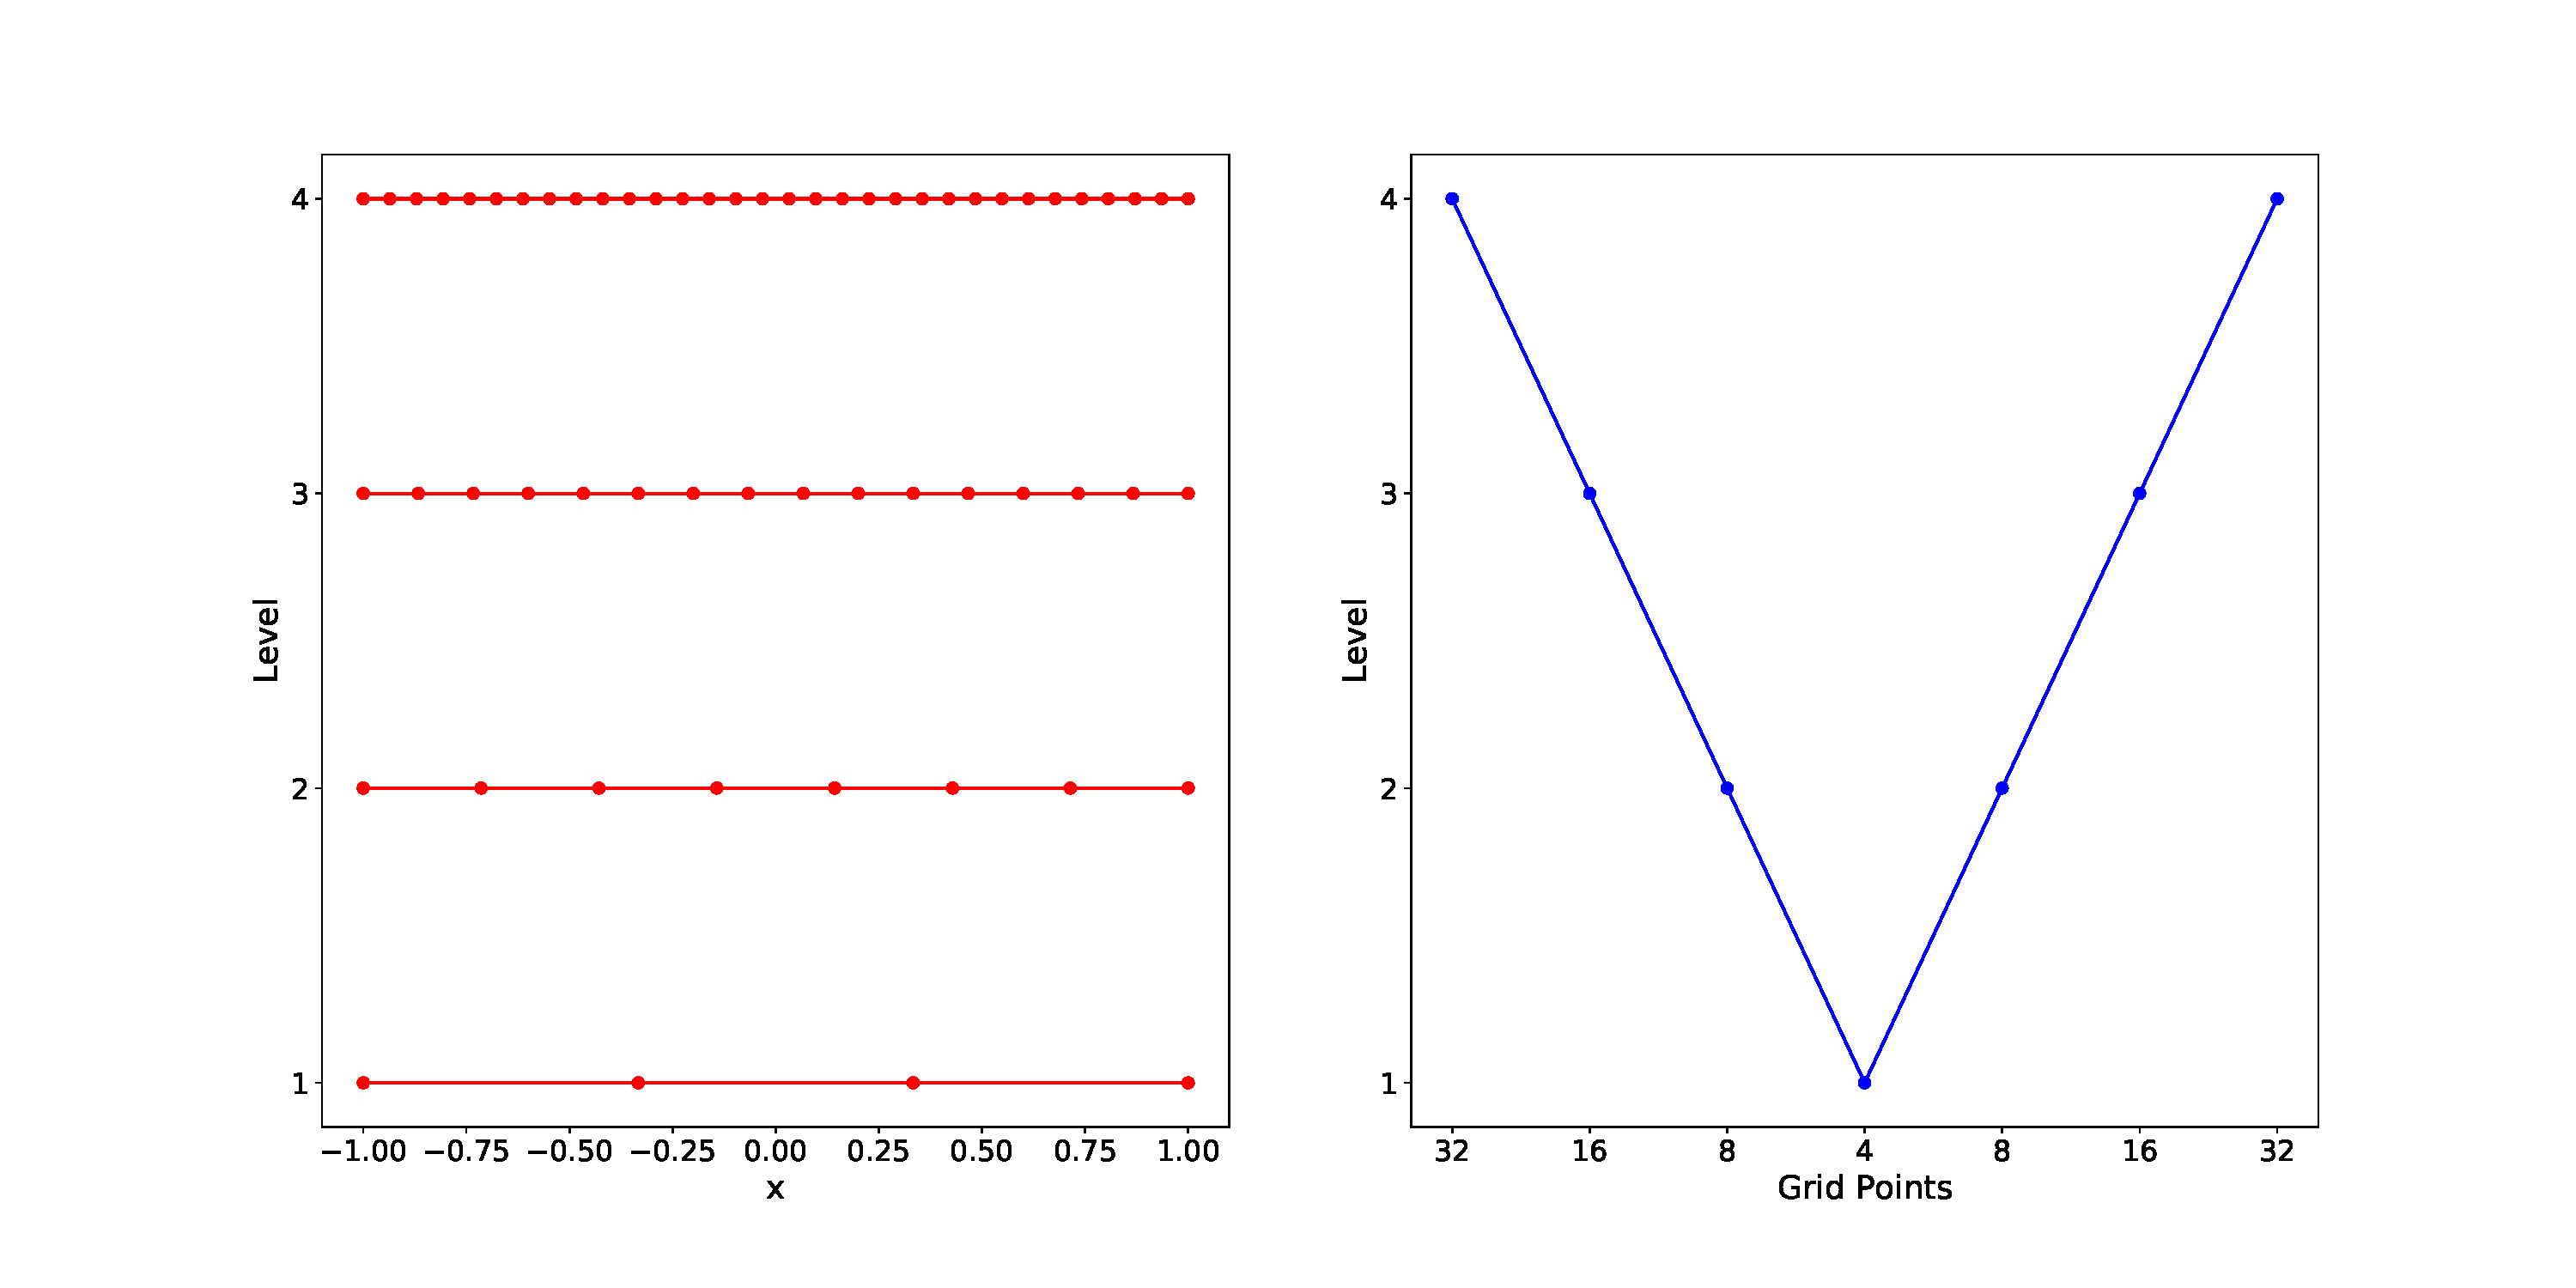
\includegraphics[width=0.8\columnwidth]{figures/multigrid.pdf}
    \caption{The 1D Multigrid Method. Starting with the finest grid, perform a few iterations of an iterative method. This is called relaxing the solution. Then project onto a coarser grid, and relax again. Do this down the levels in the grid to a desired precision. Once the solution is converged to on the coarsest level, interpolate back up the levels to obtain the solution on the finest level.}
    \label{fig:multigrid}
\end{figure}

In what is called the ``full multigrid" method, the process starts on the coarsest level instead of the finest. The solution is relaxed on this level, and then interpolated down onto a finer mesh. The interpolated solution is used as an initial guess for solving the problem on the finer mesh. The relaxed solution on a coarser grid is often an ideal initial guess for the problem on the finer mesh, resulting in quick convergence on that level.

The multigrid method allows one to accelerate an iterative solver. Multigrid methods are very effective as pre-conditioners for iterative methods. This is the general pattern of hierarchical methods: the ability to use classical iterative and direct methods on smaller grids where they perform well, and then ``scale" them up to larger problem sizes.

\subsubsection{Nested Dissection}
\label{subsub:nested-dissection}

The nested dissection method formulated by George in \cite{george1973nested} is a direct method that builds upon Gaussian elimination for problems on a grid. It is also the basis for forming what is called the multifrontal method. By taking advantage of the ordering of points on a grid, one can permute $\textbf{A}$ to first eliminate points that split the mesh into two unconnected meshes. This permutation takes the form of $\textbf{P}^* \textbf{A} \textbf{P}$, where the goal is to form $\textbf{P}$ to reorganize $\textbf{A}$ in a way that eliminates points in an efficient manner.

To detail nested dissection better, consider an $N \times N$ mesh such as a finite difference mesh discussed in Section \ref{sec:elliptic}. Assume that the initial ordering of points corresponds to an index set that iterates over the points in the mesh row-by-row. Now, the idea of nested dissection is to reorganize the points such that we first eliminate points down the middle of the mesh (i.e. the points at $x = 0$ in the first plot of Figure \ref{fig:discretization_methods}). Once these points are solved for, it spilts the mesh into two equally sized pieces that are disconnected. Each of the disconnected meshes now are smaller, and thus easier to solve. This idea of splitting the mesh into disconnected pieces by first eliminating points along an interface can be recursively applied to each split. This means that after dividing the mesh into two, one can divide those two meshes into four meshes, and so on. Recursive splitting is a common characteristic in hierarchical methods.

Nested dissection was first introduced by George in \cite{george1973nested}, and further generalized by Lipton et al. in \cite{lipton1979generalized}. Martinsson has a tutorial on nested dissection in \cite{martinsson2019fast}. In fact, nested dissection served as motivation for another hierarchical method proposed by Martinsson and Gillman called the Hierarchical Poincaré-Steklov method.

\subsubsection{The Hierarchical Poincaré-Steklov Method}
\label{subsub:hps-method}

The work done by Gillman and Martinsson in \cite{martinsson2004fast}, \cite{MARTINSSON2013460}, and \cite{gillman2014direct} (with a practical tutorial found in \cite{martinsson2015hierarchical}) culminate in what they call the Hierarchical Poincaré-Steklov (HPS) method. It is a direct solver for elliptic PDEs that is based on a binary tree of rectangular patches where the solution operator to $\textbf{A}$ is built by recursively merging child patches. Like direct methods, the HPS method involves a factorization step and a solve step. The chief advantage of the HPS method over other direct methods is that it does not require the explicit formulation and storage of $\textbf{A}$.

The HPS method starts with an original problem domain, and recursively divides the domain in half. This creates a binary tree of patches as shown in Figure \ref{fig:solve}. Once the domain has been decomposed into this tree of patches, two operators are defined on the lowest level, called the leaf level. These operators are the solution operator $\textbf{S}$ and Dirichlet-to-Neumann (DtN) operator $\textbf{T}$. The solution operator maps boundary data to solution data on the interior of the patch (i.e. solves the local boundary value problem), and the DtN operator maps Dirichlet data on the boundary to Neumann data on the boundary. These operators can be formed using any elliptic PDE solver, including fast solvers like spectral methods. After forming these operators, the next step is to recursively merge each sibling patch up the tree. the merge step is demonstrated in Figure \ref{fig:merge}. This results in a global solution operator that can be stored and used multiple times (at different time steps or with varying boundary conditions, etc.), and is similar to a direct method matrix factorization. The final step is applying the solution operator to each level down the tree to obtain the solution everywhere in the domain. This step is just a matrix-vector multiplication and is very fast.

Similar to other direct methods, the HPS method forms an in-memory solution operator that can be applied to several right-hand side vectors. This property makes it ideal for problems where several elliptic solves are necessary. While most iterative methods have better asymptotic performance than other direct methods, the HPS method can be accelerated using hierarchically block seperable (HBS) matrix algebra to achieve near linear asymptotic performance (\cite{gillman2014direct}).

\begin{figure}
    \centering
    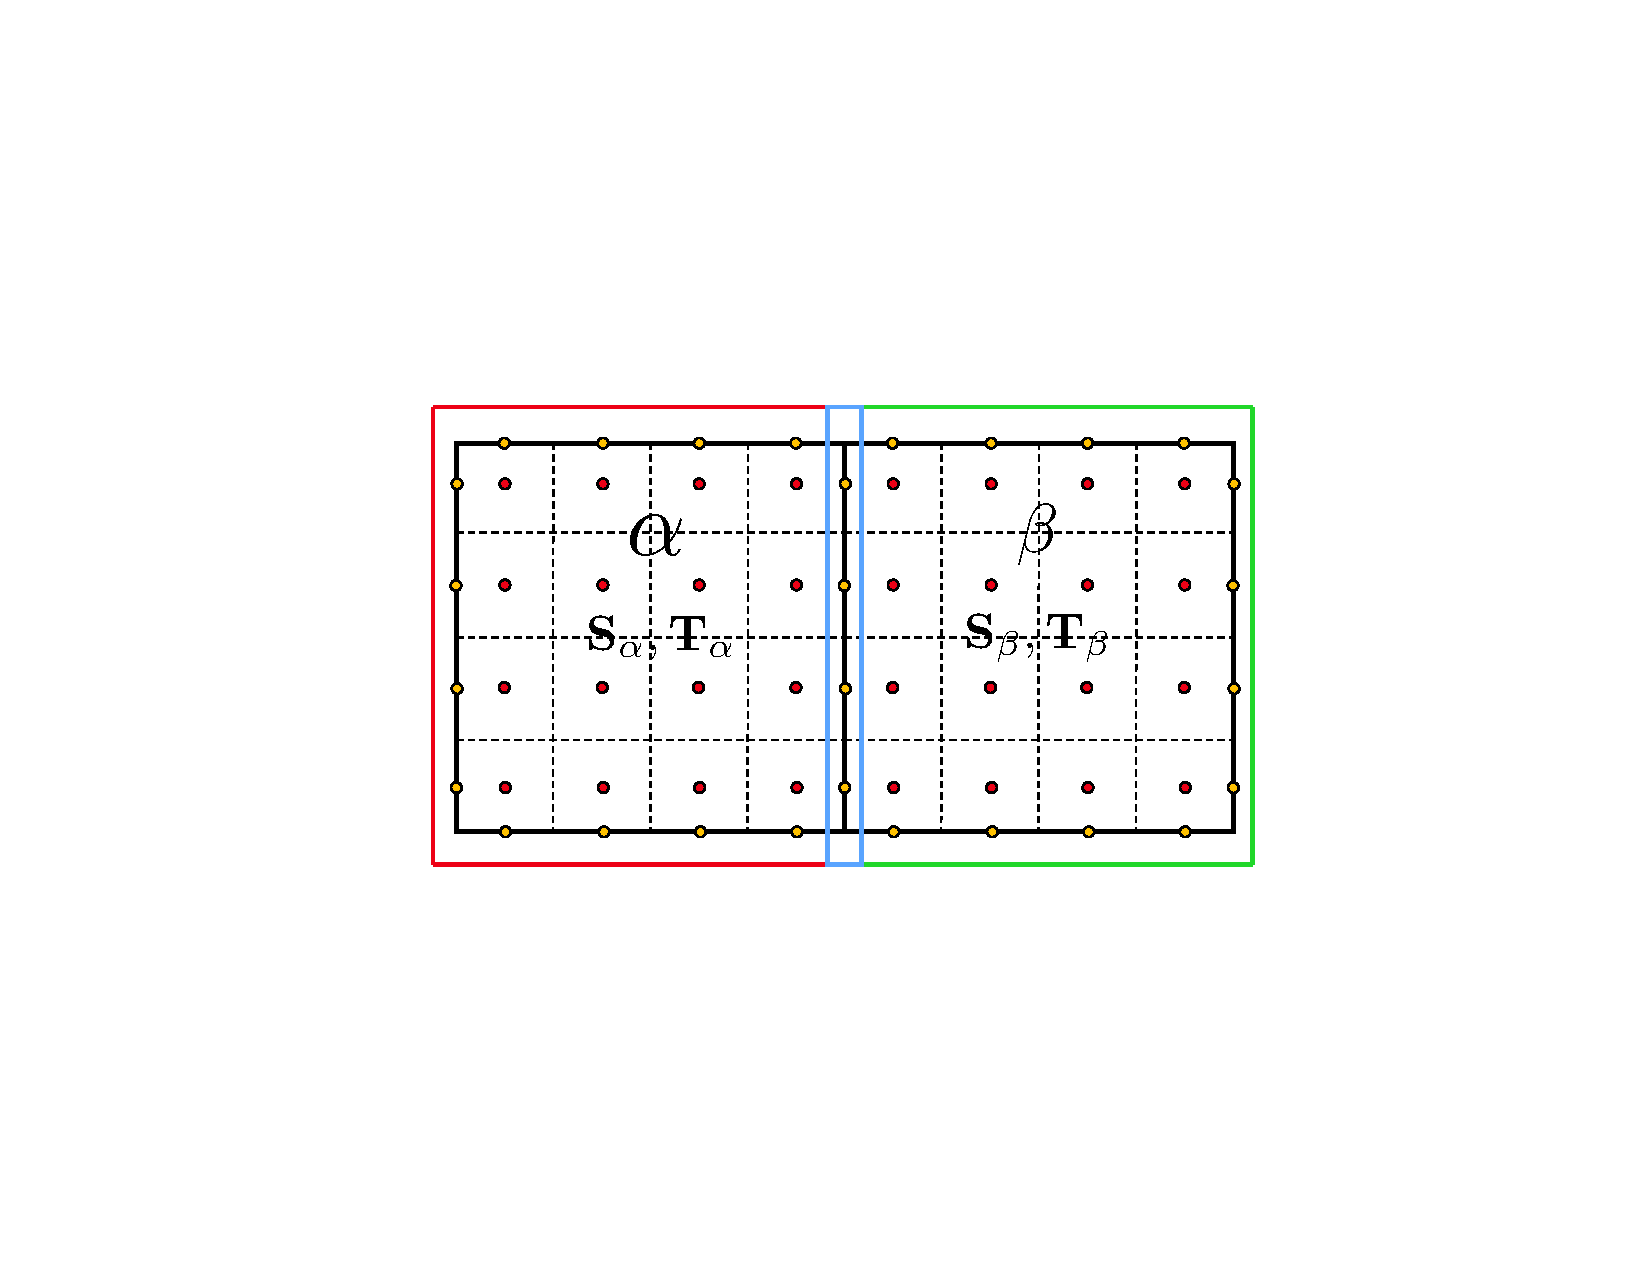
\includegraphics[width=0.7\columnwidth]{figures/merge_figure.pdf}
    \caption{HPS Merge Operation. The merged patch $\Omega_{\tau}$ is the union of children $\Omega_{\alpha}$ and $\Omega_{\beta}$, i.e. $\Omega_{\tau} = \Omega_{\alpha} \cup \Omega_{\beta}$. Red, green, and blue nodes correspond to index sets $\textbf{I}_1$, $\textbf{I}_2$, and $\textbf{I}_3$, respectively. The merge operation eliminates the nodes on the interface of the children patches.}
    \label{fig:merge}
\end{figure}

\begin{figure}
    \centering
    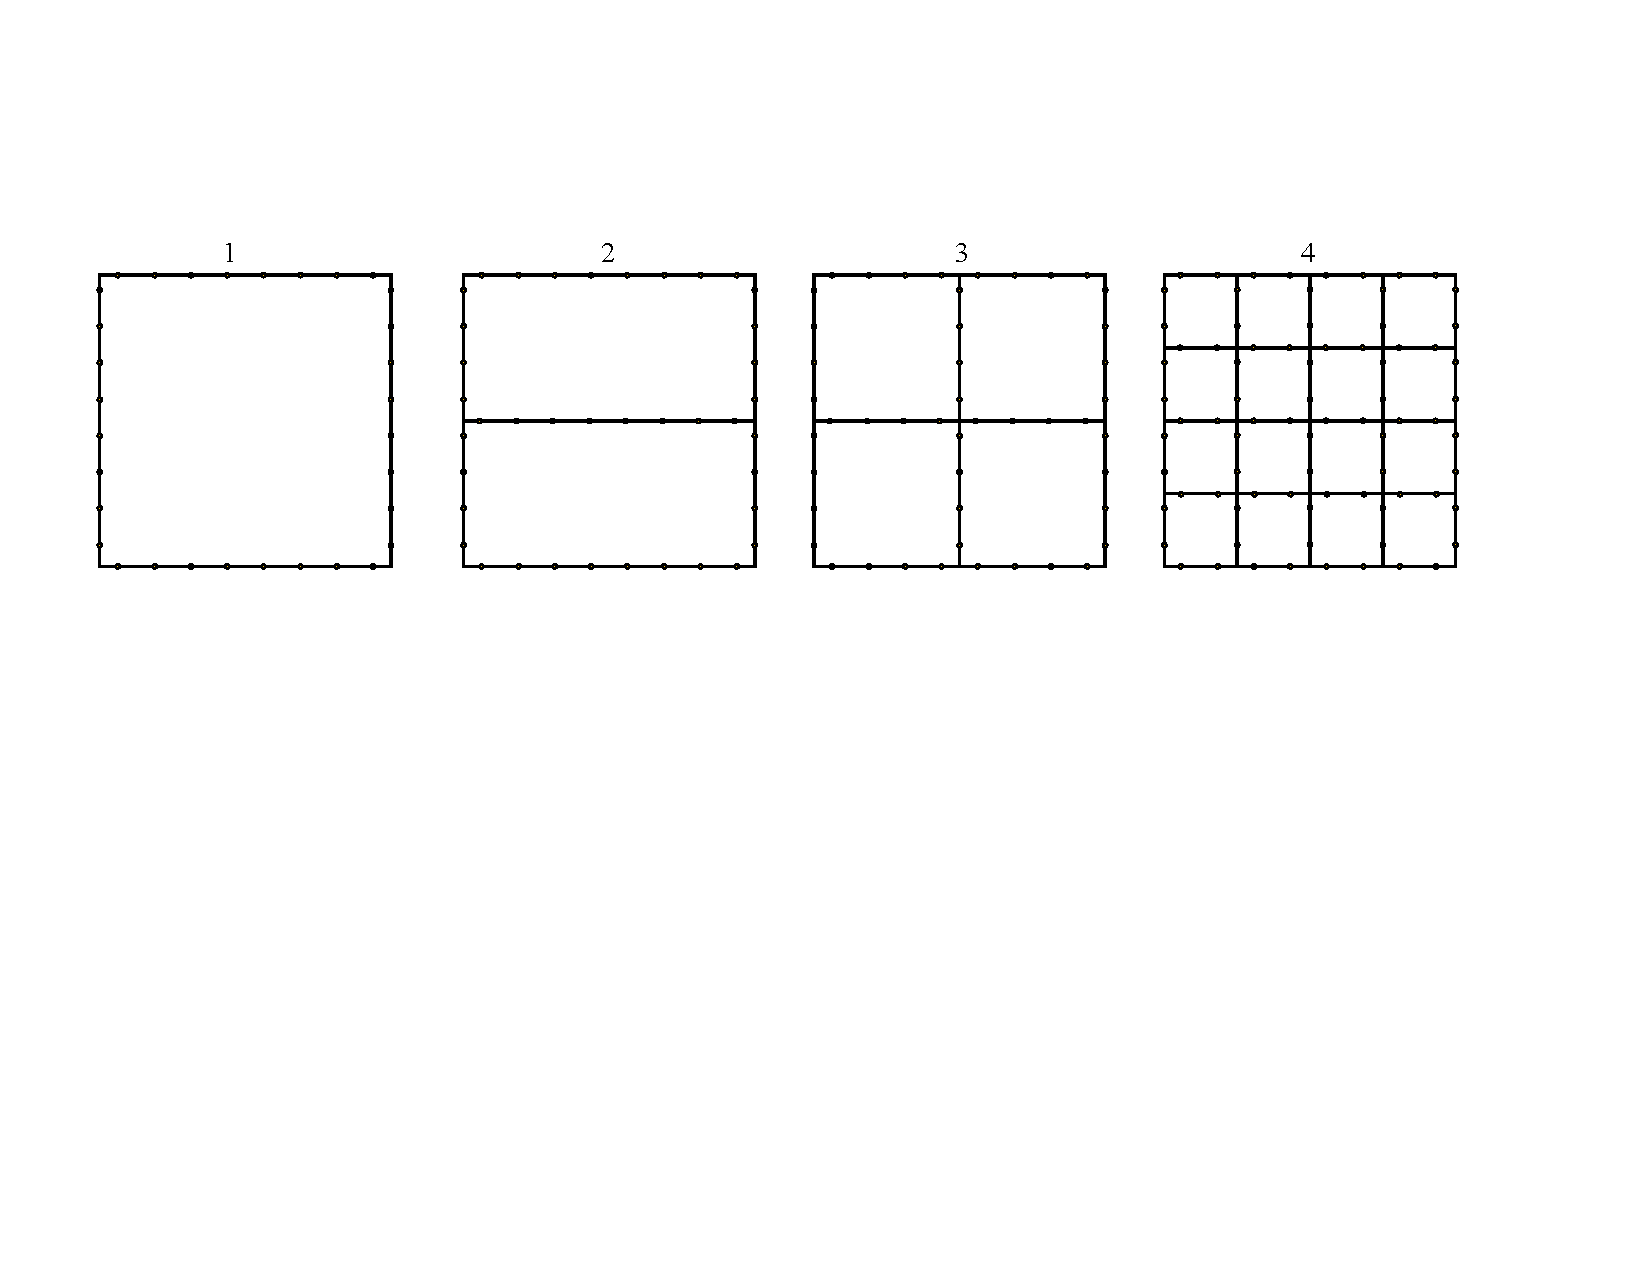
\includegraphics[width=\columnwidth]{figures/solve_figure.pdf}
    \caption{HPS Solve Stage. Once $\textbf{S}_0$ is formed, apply it to the top level Dirichlet data to get boundary (and solution) data on the interface of the children. Apply the patch solution operator down the tree until each leaf has it's local boundary information. Then apply the solution operator to get the solution data in the interior of each leaf.}
    \label{fig:solve}
\end{figure}


\chapter{The Quadtree-Adaptive HPS Method}
\label{chap:qahps}
\section{Introduction}
\label{sec:intro}

The \gls{qahps} method is a direct method for solving elliptic \gls{pdes} on a hierarchy of adaptively refined finite volume meshes. It builds upon the \gls{hps} methods first presented by \citet{gillman2014direct}, including \gls{amr} considerations found in \citep{babb2018accelerated,geldermans2019adaptive}. The primary contribution of the \gls{qahps} method is the derivation and implementation of the \gls{hps} method for use with a quadtree-style mesh with embedded finite volume meshes. In this chapter, we will derive the \gls{qahps} method, detail the implementation for use with \pforest \citep{burstedde2011p4est,burstedde2020parallel}, and provide a detailed convergence and error analysis for elliptic \gls{pdes}.
\section{Problem Statement}
\label{sec:problem-statement}

The general problem we wish to solve is the variable coefficient elliptic \gls{pde} that we define as
\begin{align}
    \label{eq:elliptic-pde}
    \mathcal{A}[u(\textbf{x})] \equiv \nabla \cdot \left( \beta(\textbf{x}) \nabla u(\textbf{x}) \right) + \lambda(\textbf{x}) u(\textbf{x}) &= f(\textbf{x}), \quad \textbf{x} \in \Omega \subset \mathcal{R}^2
\end{align}
subject to either Dirichlet or Neumann boundary conditions:
\begin{align}
    \label{eq:elliptic-pde-bc1}
    u(\textbf{x}) &= g(\textbf{x}), \quad \textbf{x} \in \Gamma_D \subset \Omega \quad \mbox{or}\\
    \label{eq:elliptic-pde-bc2}
    \frac{\partial u}{\partial n} \Big|_{\textbf{x}} &= v(\textbf{x}), \quad \textbf{x} \in \Gamma_N \subset \Omega.
\end{align}

\begin{figure}
    \centering
    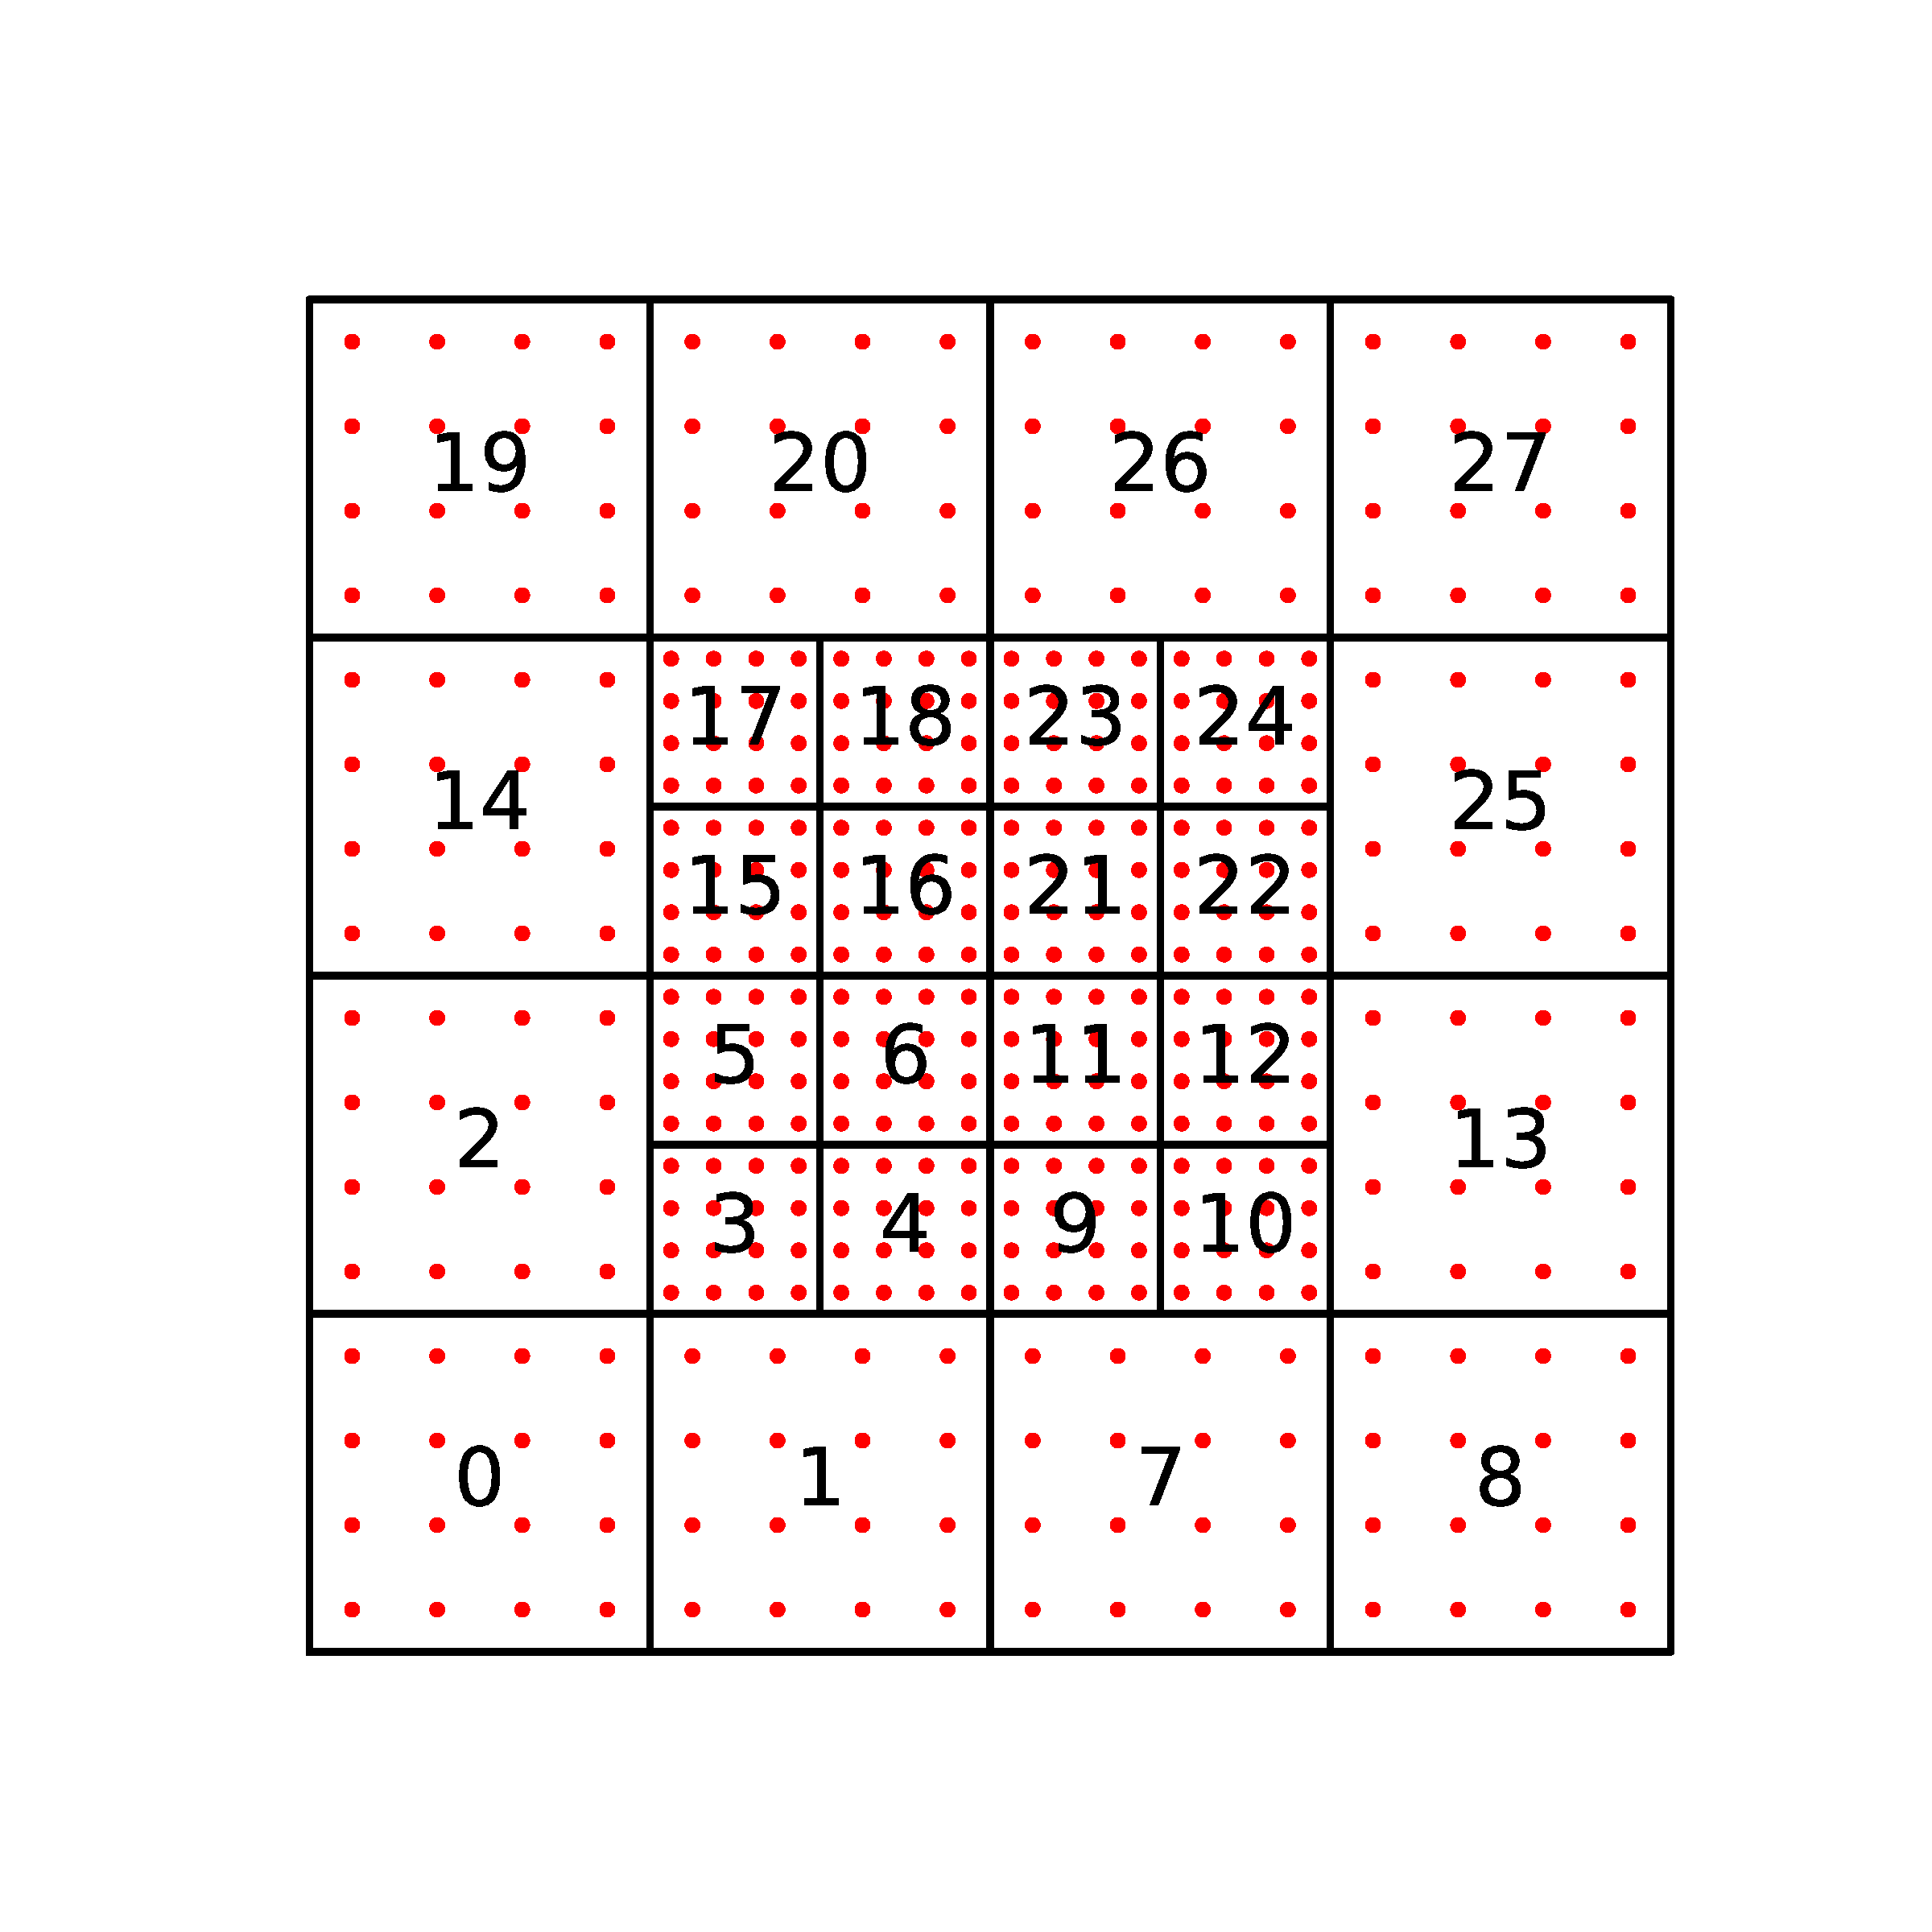
\includegraphics[width=\textwidth, clip=true, trim={0 160 0 160}]{figures/adaptive-mesh-serial.pdf}
    \caption{An example of a domain $\Omega$ refined according to a refinement criteria that refines around the center of the domain. The indices indicate the leaf-level index as organized into a leaf-level quadtree $\mathcal{Q}_L$. Each subdomain has a finite volume discretization associated with it as depicted with the red points.}
    \label{fig:adaptive-mesh-serial}
\end{figure}

The domain $\Omega$ is partitioned into a composite collection of subdomains $\Omega_i$ such that $\Omega = \cup_{i = 1}^{N} \Omega_i$. This is displayed in \reffig{fig:adaptive-mesh-serial}. These subdomains are organized into a {\em leaf-indexed quadtree}
\begin{align}
    \mathcal{Q}_L = \{\Omega_i | i = 1, \dots, N_L\},
    \label{eq:leaf-indexed-quadtree}
\end{align}
where $N_L$ is the number of leaf nodes. \ignore{A representation of the mesh in \reffig{fig:adaptive_mesh} as a leaf-indexed quadtree can be found in \reffig{subfig:leaf-indexed-quadtree}.} Building up $\mathcal{Q}_L$ is done by recursively refining a logically square domain into children patches according a refinement criteria (or tagging criteria)
\begin{align}
    T_{R} (\textbf{x}) =
    \begin{cases}
        1,& \eta(\textbf{x}) > \epsilon_{R} \\
        0,& \text{otherwise},
    \end{cases}
    \quad \textbf{x} \in \Omega_i
\end{align}
where $\eta(\textbf{x})$ is a metric used to measure the need for refinement such as error or state variable gradient. $1$ indicates refinement and $0$ indicates no refinement. The user-defined variable $\epsilon_{R}$ is the refinement threshold. While a coarsening criteria $T_{C}$ is also defined similar to the refinement criteria, it is often not used in the initialization of $\mathcal{Q}_L$.

We also define a {\em path-indexed quadtree} that is formally denoted as
\begin{align}
    \mathcal{Q}_P = \{\Omega^{\tau} | \tau = 1, \dots, N_P\},
    \label{eq:path-indexed-quadtree}
\end{align}
where $\tau$ is a key that indicates the path of a node in $\mathcal{Q}_P$ and $N_P$ is the number of nodes in $\mathcal{Q}_P$. The primary difference between a leaf-indexed quadtree and a path-indexed quadtree is the indexing of nodes; a leaf-indexed quadtree has data storage for only leaf nodes while a path-indexed quadtree has data storage for all nodes in the quadtree (leaves and ancestors). Both types of trees are depicted in \reffig{fig:quadtree-indexing-serial}.

\begin{figure}
    \centering
    \begin{tabular}{c}
    \smallskip
        \begin{subfigure}[t]{0.8\textwidth}
            \centering
            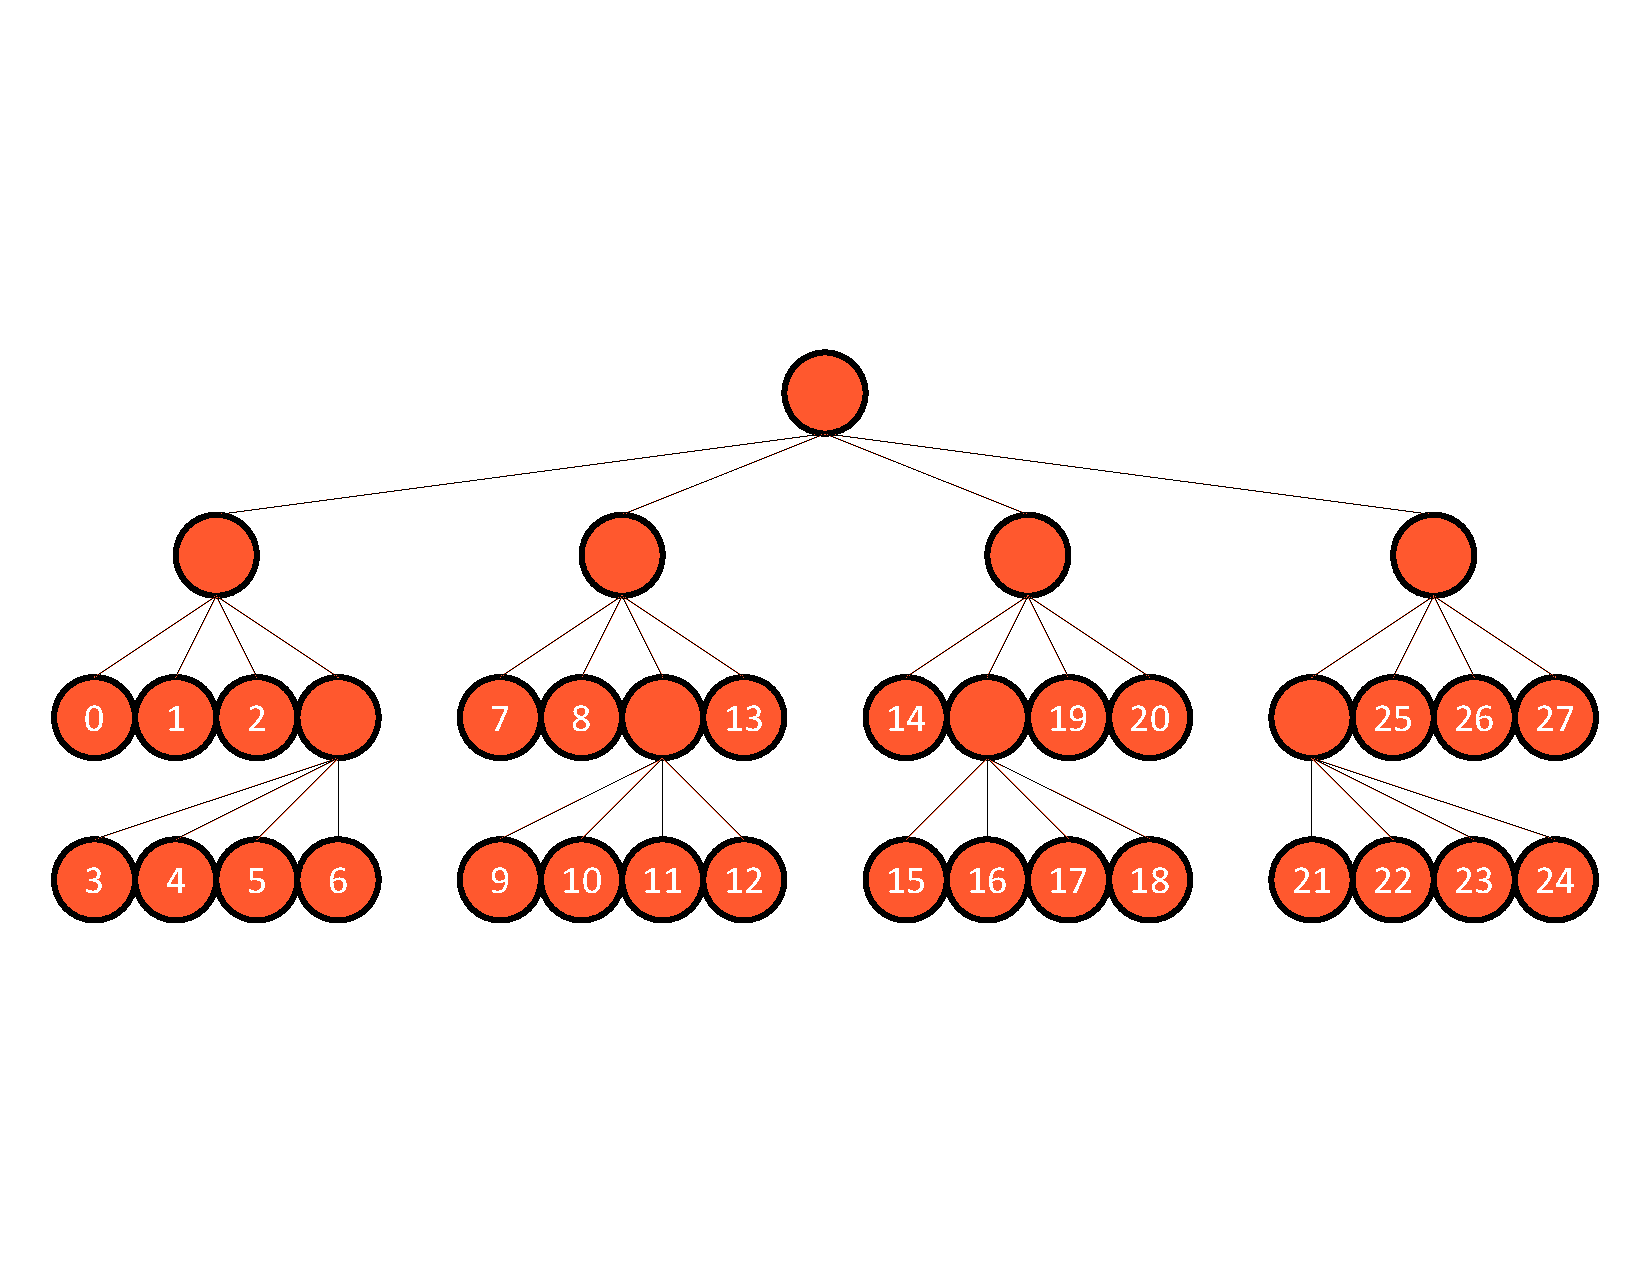
\includegraphics[width=\textwidth, clip=true, trim={0 150 0 150}]{figures/leaf-indexed-quadtree-serial.pdf}
            \caption{Leaf-indexed quadtree $\mathcal{Q}_L$}
            \label{subfig:leaf-indexed-quadtree-serial}
        \end{subfigure}
        \\
        \begin{subfigure}[t]{0.8\textwidth}
            \centering
            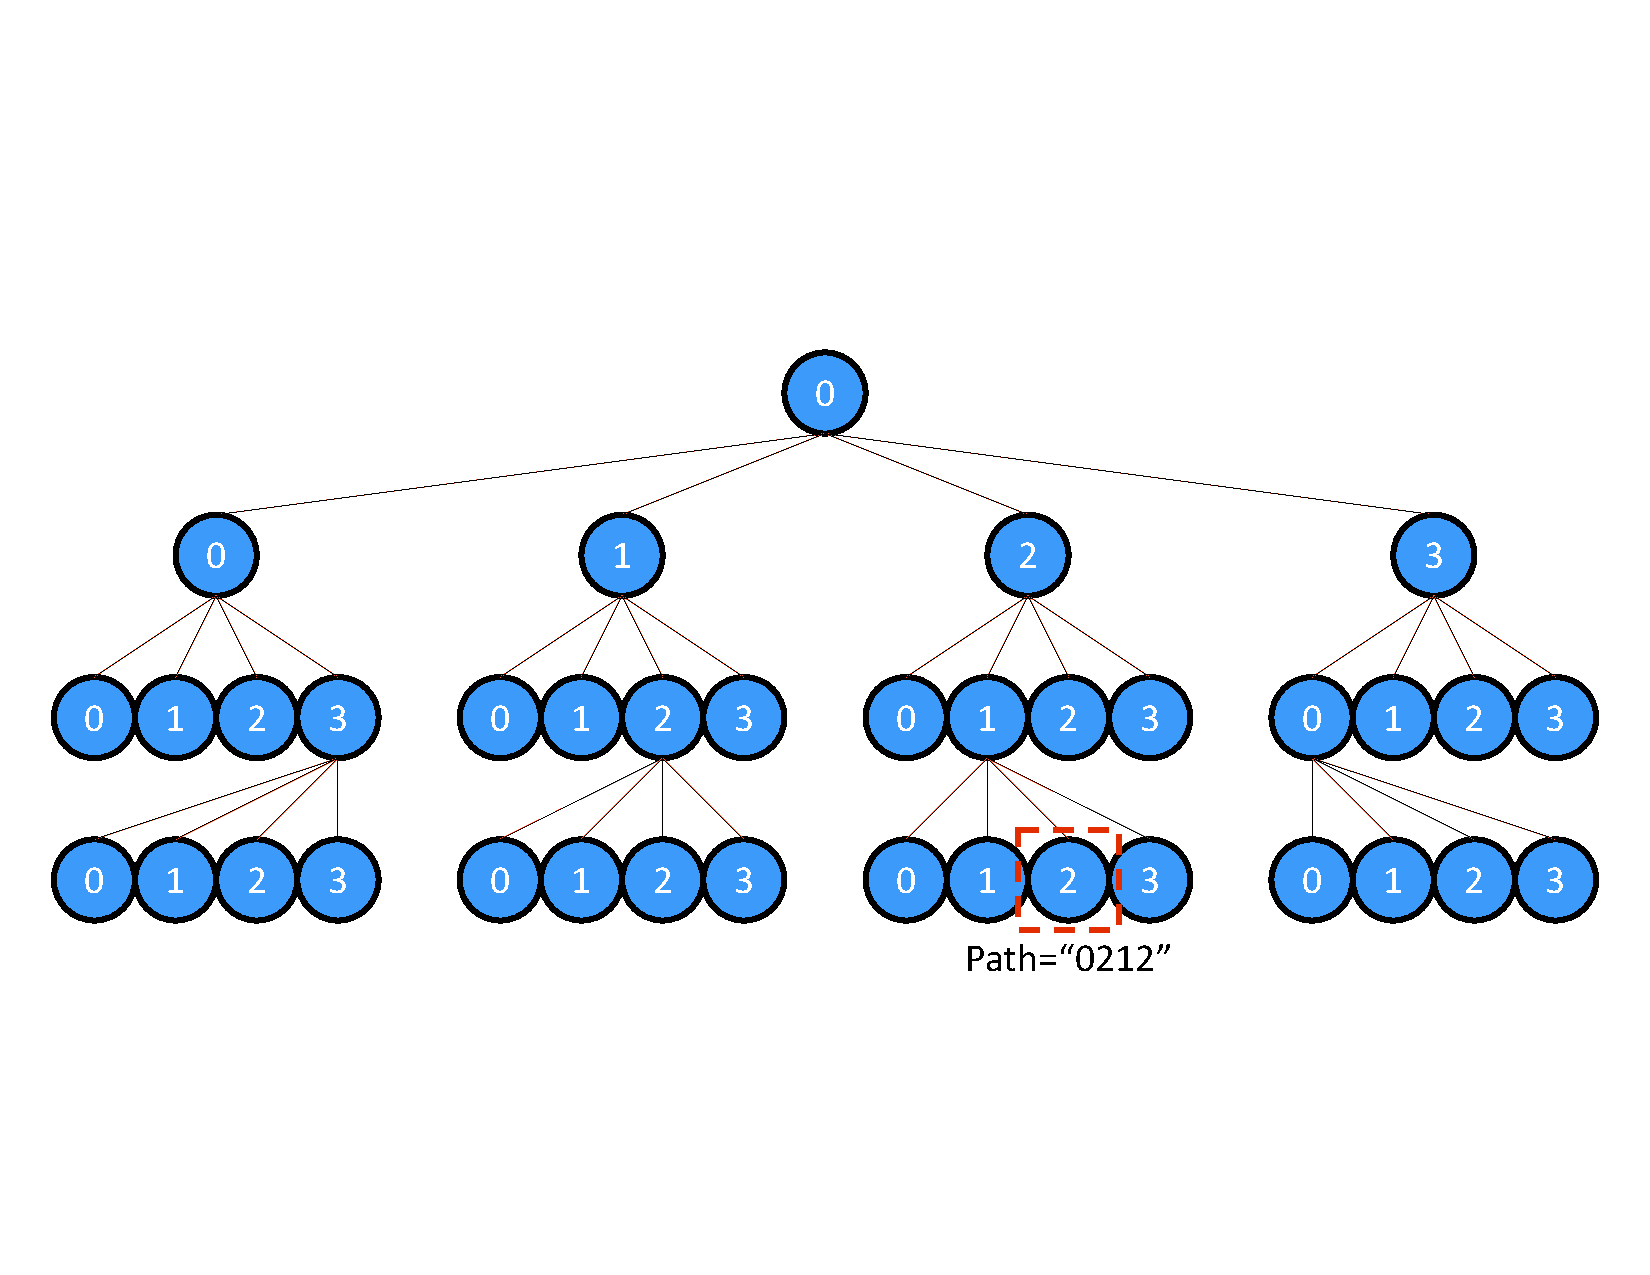
\includegraphics[width=\textwidth, clip=true, trim={0 140 0 150}]{figures/path-indexed-quadtree-serial.pdf}
            \caption{Path-indexed quadtree $\mathcal{Q}_P$}
            \label{subfig:path-indexed-quadtree-serial}
        \end{subfigure}
    \end{tabular}\\
    \caption{Leaf-indexed vs. path-indexed quadtrees. These represent the domain shown in \reffig{fig:adaptive-mesh-serial}. Note that the leaf-indexed quadtree only stores the leaf nodes (nodes without children), while the path-indexed quadtree stores all nodes (leaf and intermediate nodes).}
    \label{fig:quadtree-indexing-serial}
\end{figure}

% We focus on the constant coefficient elliptic problem
% \begin{equation}
%     \nabla^2 u(x,y) + \lambda u(x,y) = f(x,y), \quad \lambda \ge 0
%     \label{eq:elliptic_pde}
% \end{equation}
% with $(x,y) \in \Omega = [a, b] \times [c,d]$, subject to Dirichlet boundary conditions
% \begin{equation}
%     u(x,y) = g(x,y),\ \ (x,y) \in \Gamma = \partial \Omega.
% \end{equation}
% For this paper, we assume that $b-a=d-c$ so that we can describe our mesh using a single quadtree and square mesh cells.  In general though, this is not a limitation of meshes generated using the multi-block ``forest-of-octrees'' capabilities of \pforest.  The primary contributions of this paper are an HPS solver for the constant coefficient ellitpic problem on an adaptively refined \pforest mesh. In future work, we will include fast linear algebra needed to reduce the complexity of the overall algorithm to $\mathcal O(N)$, a key contribution of the original HPS method developed by Gillman and Martinsson.
\section{Components of the HPS algorithm : Merging, Splitting and Leaf Computations}
\label{sec:quadtree}

The \gls{qahps} method applied to \refeq{eq:elliptic-pde} is broken into a factorization stage (called the build stage) and an application stage (called the solve stage). For problems in which $f(x,y)$ is non-zero, an additional ``upwards'' stage is required which handles the inhomogeneous correction.

The goal of the \gls{qahps} method is to build up a {\em solution operator set} defined as
\begin{align}
    \mathcal{S} = \{(\textbf{S}^{\tau}, \textbf{w}^{\tau}) : \ \forall\ \tau \in \mathcal{Q}_P\}
    \label{eq:solution-operator-set}
\end{align}
where \Stau and \wtau are the solution operator and the inhomogeneous correction, respectively, which can then be applied to supplied Dirichlet data \gtau such that
\begin{align}
    \textbf{u}^{\tau} = \textbf{S}^{\tau} \textbf{g}^{\tau} + \textbf{w}^{\tau},\ \forall\ \tau \in \mathcal{Q}_P.
    \label{eq:u-Sg-w}
\end{align}
Building up the solution operator set is done by successively merging child-level \gls{d2n} operators \Ttau through the computation of a Schur complement.

Each stage of the \gls{qahps} method has a leaf-level computation associated with it, as well as a 4-to-1 merge algorithm (for the build and upwards stages) or a 1-to-4 split algorithm (for the solve stage). The follows sections detail each of these in turn.

\subsection{Leaf Level Computations}
\label{sub:leaf_level_computations}

In what follows, we assume that each leaf-level quadrant in the quadtree mesh stores a uniform Cartesian grid with $M \times M$ mesh cells.  We refer to this local Cartesian mesh, along with its quadrant as a {\em patch}.  In \reffig{fig:4_to_1_patches} (left), we show four patches in a larger composite domain. Cell-centered finite difference schemes are particularly convenient for adaptively refined Cartesian meshes, since the cell-centered values are not duplicated on adjacent patches.

At the leaf-level, the build stage of the HPS methods requires the solution to a Poisson problem \eqn{elliptic-pde} discretized on an $M \times M$ cell-centered grid as
\begin{equation}
\Atau \utau = \Bctau \gtau + \ftau
\label{eq:patch_poisson_problem}
\end{equation}
where $\Bctau$ spreads Dirichlet boundary data $\gtau \in \real^{4M}$ to the grid and \ftau is the right hand side function $f(x,y)$ from \eqn{elliptic-pde} evaluated at cell centers.  We write the solution to this problem in terms of a {\em homogeneous operator} \Lhtau and an inhomogeneous operator \Linhtau which represent efficient solvers on the uniform Cartesian patch. The solution is then given by 
\begin{equation}
\utau = \Lhtau \gtau + \Linhtau \ftau
\label{eq:patch_leaf_solve}
\end{equation}
Where the context is clear, we also view operators \Lhtau and \Linhtau, boundary data \gtau and right hand side data \ftau as matrices and vectors of the appropriate sizes. The components of \utau are given by $u^\tau_{ij}$, for $i,j = 1,2,\hdots M$.  

Using these leaf-level solvers, we can now build a leaf-level DtN operator \Ttau.  In the description below, we illustrate the HPS method on the complete Poisson problem, assuming a non-zero right hand side.  We remark below, though, that if one anticipates solving for multiple right-hand sides, the build stage can be separated into a factorization stage and an "upwards" stage to handle inhomogeneous data.  

\ignore{\donna{Not sure where to put this.}  The general HPS algorithm does not specify a particular local mesh discretization, and several have been proposed in the literature.  In \citep{gillman2014direct}, the authors use a spectral collocation method and in \citep{fortunato2020ultraspherical}, a Chebyshev tensor product grid for high order finite elements was used. For compatibility with the finite volume code ForestClaw \citep{calhoun2017forestclaw}, we use a second order finite volume discretization of \refeq{eq:elliptic-pde}.}

\subsubsection{\DtN (DtN) operator}
Given a cell-centered grid solution $\utau = \Lhtau \gtau + \Linhtau \ftau$, we define ``interior" grid values $\uin \in \real^{4M}$ as those grid solution values \utau for which $i = 1$, $i = M$, $j = 1$ or $j = M$.  By analogy, components of \uout are grid solution values for which $i=0$ or $i = M+1$ or $j = 0$ or $j = M+1$.     

On a cell-centered finite volume grid, the known Dirichlet boundary values are not collocated with components of the grid solution so we discretize the Dirichlet boundary condition at the midpoint between \ukin and \ukout as
\begin{equation}
g_k^\tau = \frac{\ukout + \ukin}{2}, \quad k = 1,\hdots , 4M
\end{equation}
where $g_k$, $\ukin$ and $\ukout$ are the components of \gtau, \uin and \uout respectively.  

By analogy, we discretize Neumann data on the boundary of the patch as
\begin{equation}
v_k = \frac{\ukout - \ukin}{h}
\end{equation}
where $h$ is the mesh cell width (assumed to be uniform in both x- and y- directions).

Eliminating $\ukout$  between the two expressions, we  can express the Neumann data $v_k$ in terms of Dirichlet data $g_k$ and the interior value $\ukin$ as
\begin{equation}
v_k = \frac{2}{h}(g_k - \ukin).
\end{equation}
The vector of Neumann data on patch $\tau$ can then be expressed as 
\begin{equation}
\vtau = \frac{2}{h}(\gtau - \uin).
\end{equation}   

Introducing an operator (or a matrix of the appropriate size) \Gop that selects \uin from the grid solution data \utau, we write $\uin = \Gop \utau$ so that
\begin{equation}
\vtau = \frac{2}{h}(\gtau - \Gop (\Lhtau \gtau + \Linhtau \ftau) = 
\frac{2}{h}(I - \Gop \Lhtau)\gtau - \frac{h}{2}\Gop \Linhtau \ftau
\end{equation}
From this, we define the leaf level \DtN mapping $\Ttau \in \real^{4M \times 4M}$ as
\begin{equation}
\Ttau \equiv \frac{2}{h}(I - \Gop\Lhtau).
\label{eq:Ttau-leaf}
\end{equation}
with inhomogenenous component
\begin{equation}
\htau \equiv -\frac{2}{h}\Gop\Linhtau \ftau.
\label{eq:htau-leaf}
\end{equation}
Neumann data on the patch is then computed as
\begin{equation}
\vtau = \Ttau \gtau + \htau.
\label{eq:vtau}
\end{equation}
We refer \Ttau as a discrete \DtN operator, although the Neumann data \vtau is not the Neumann data that is commonly understood to be the result of applying a DtN map, since \vtau depends not only on the Dirichlet data \gtau, but also on the inhomogeneous data \ftau.  

\subsection{The 4-to-1 Merge Algorithm}
\label{sub:4-to-1merge}
If $\tau$ is not a leaf-level quadrant, then we construct the DtN map \Ttau {\em recursively} by merging mappings from the four children patches $\alpha$, $\beta$, $\gamma$ and $\omega$  partitioning $\tau$.  For the non-leaf, two additional operators $\Stau$ and $\Xtau$ (for non-zero $f(x,y)$) are also constructed.  Prior to this merge process, it is assumed that each patch has computed a DtN mapping \Ti, for $i=\alpha$, $\beta$, $\gamma$, $\omega$. 

\begin{figure}
    \centering
    \begin{tabular}{ccc}
        \begin{subfigure}[t]{0.3\textwidth}
            \centering
            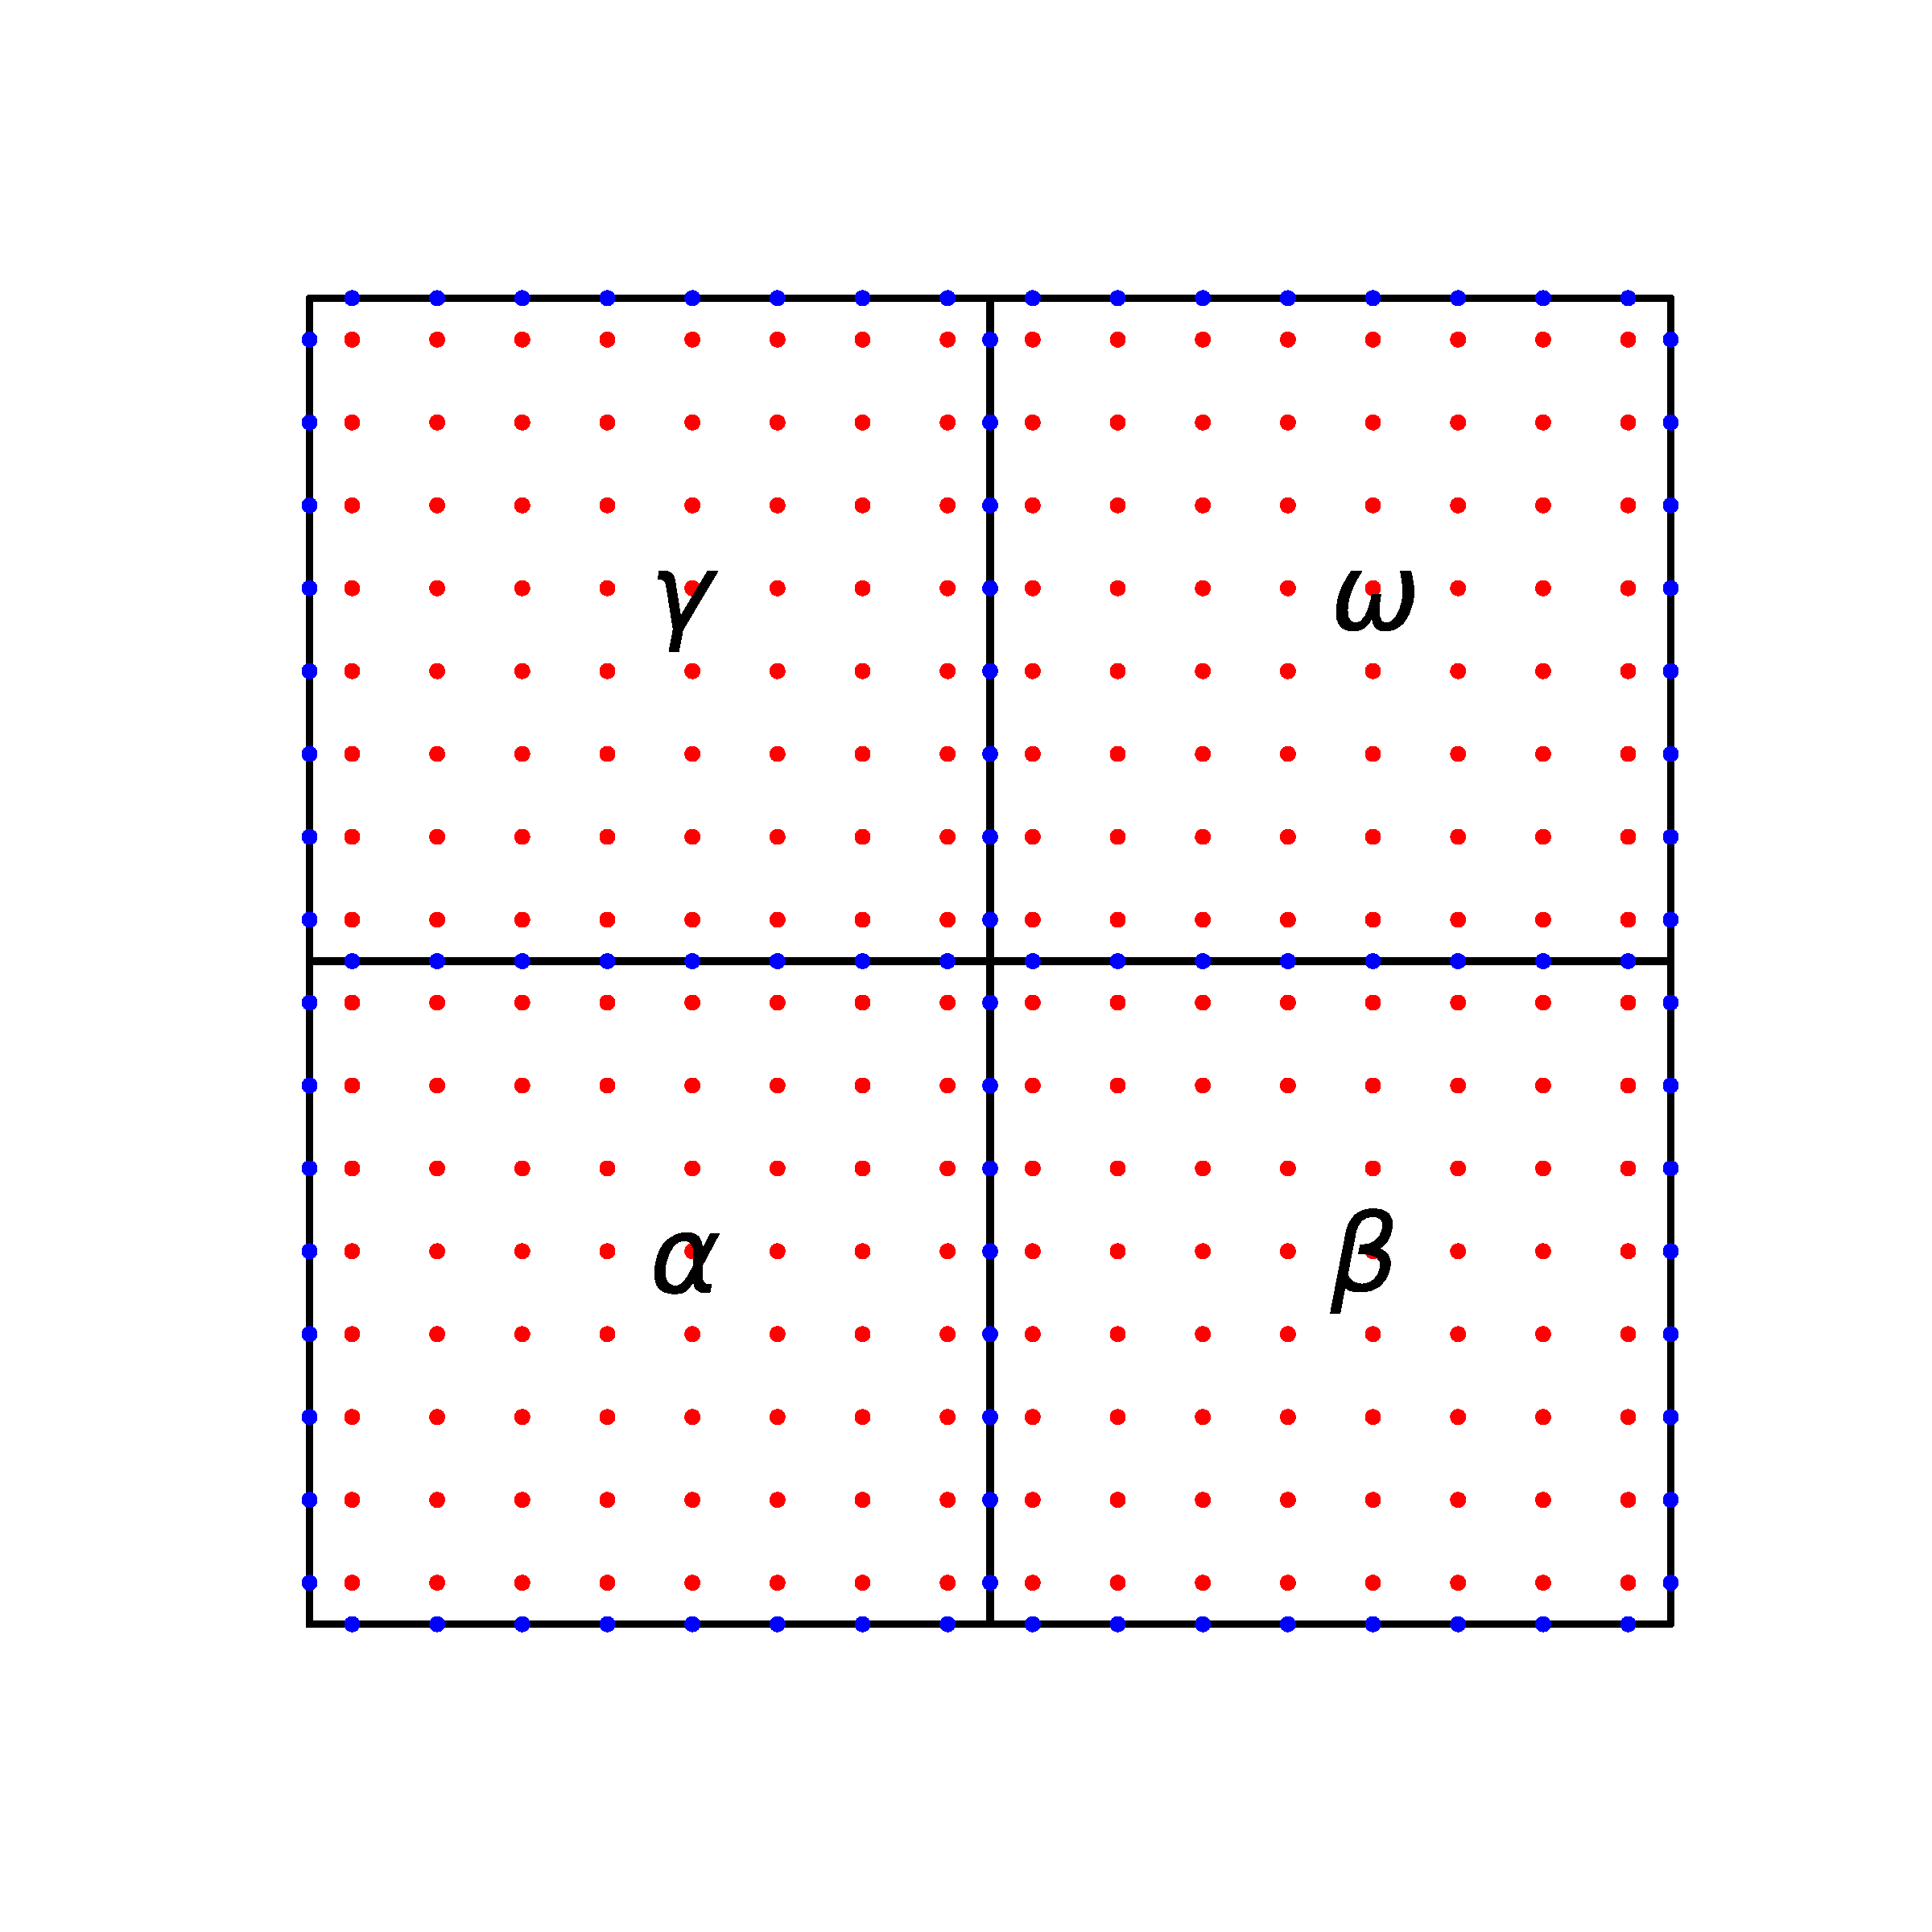
\includegraphics[width=\textwidth, clip=true, trim={100 150 100 150}]{figures/four_patches.pdf}
            \label{subfig:4_patches_with_grid}
        \end{subfigure}
        &
        \begin{subfigure}[t]{0.3\textwidth}
            \centering
            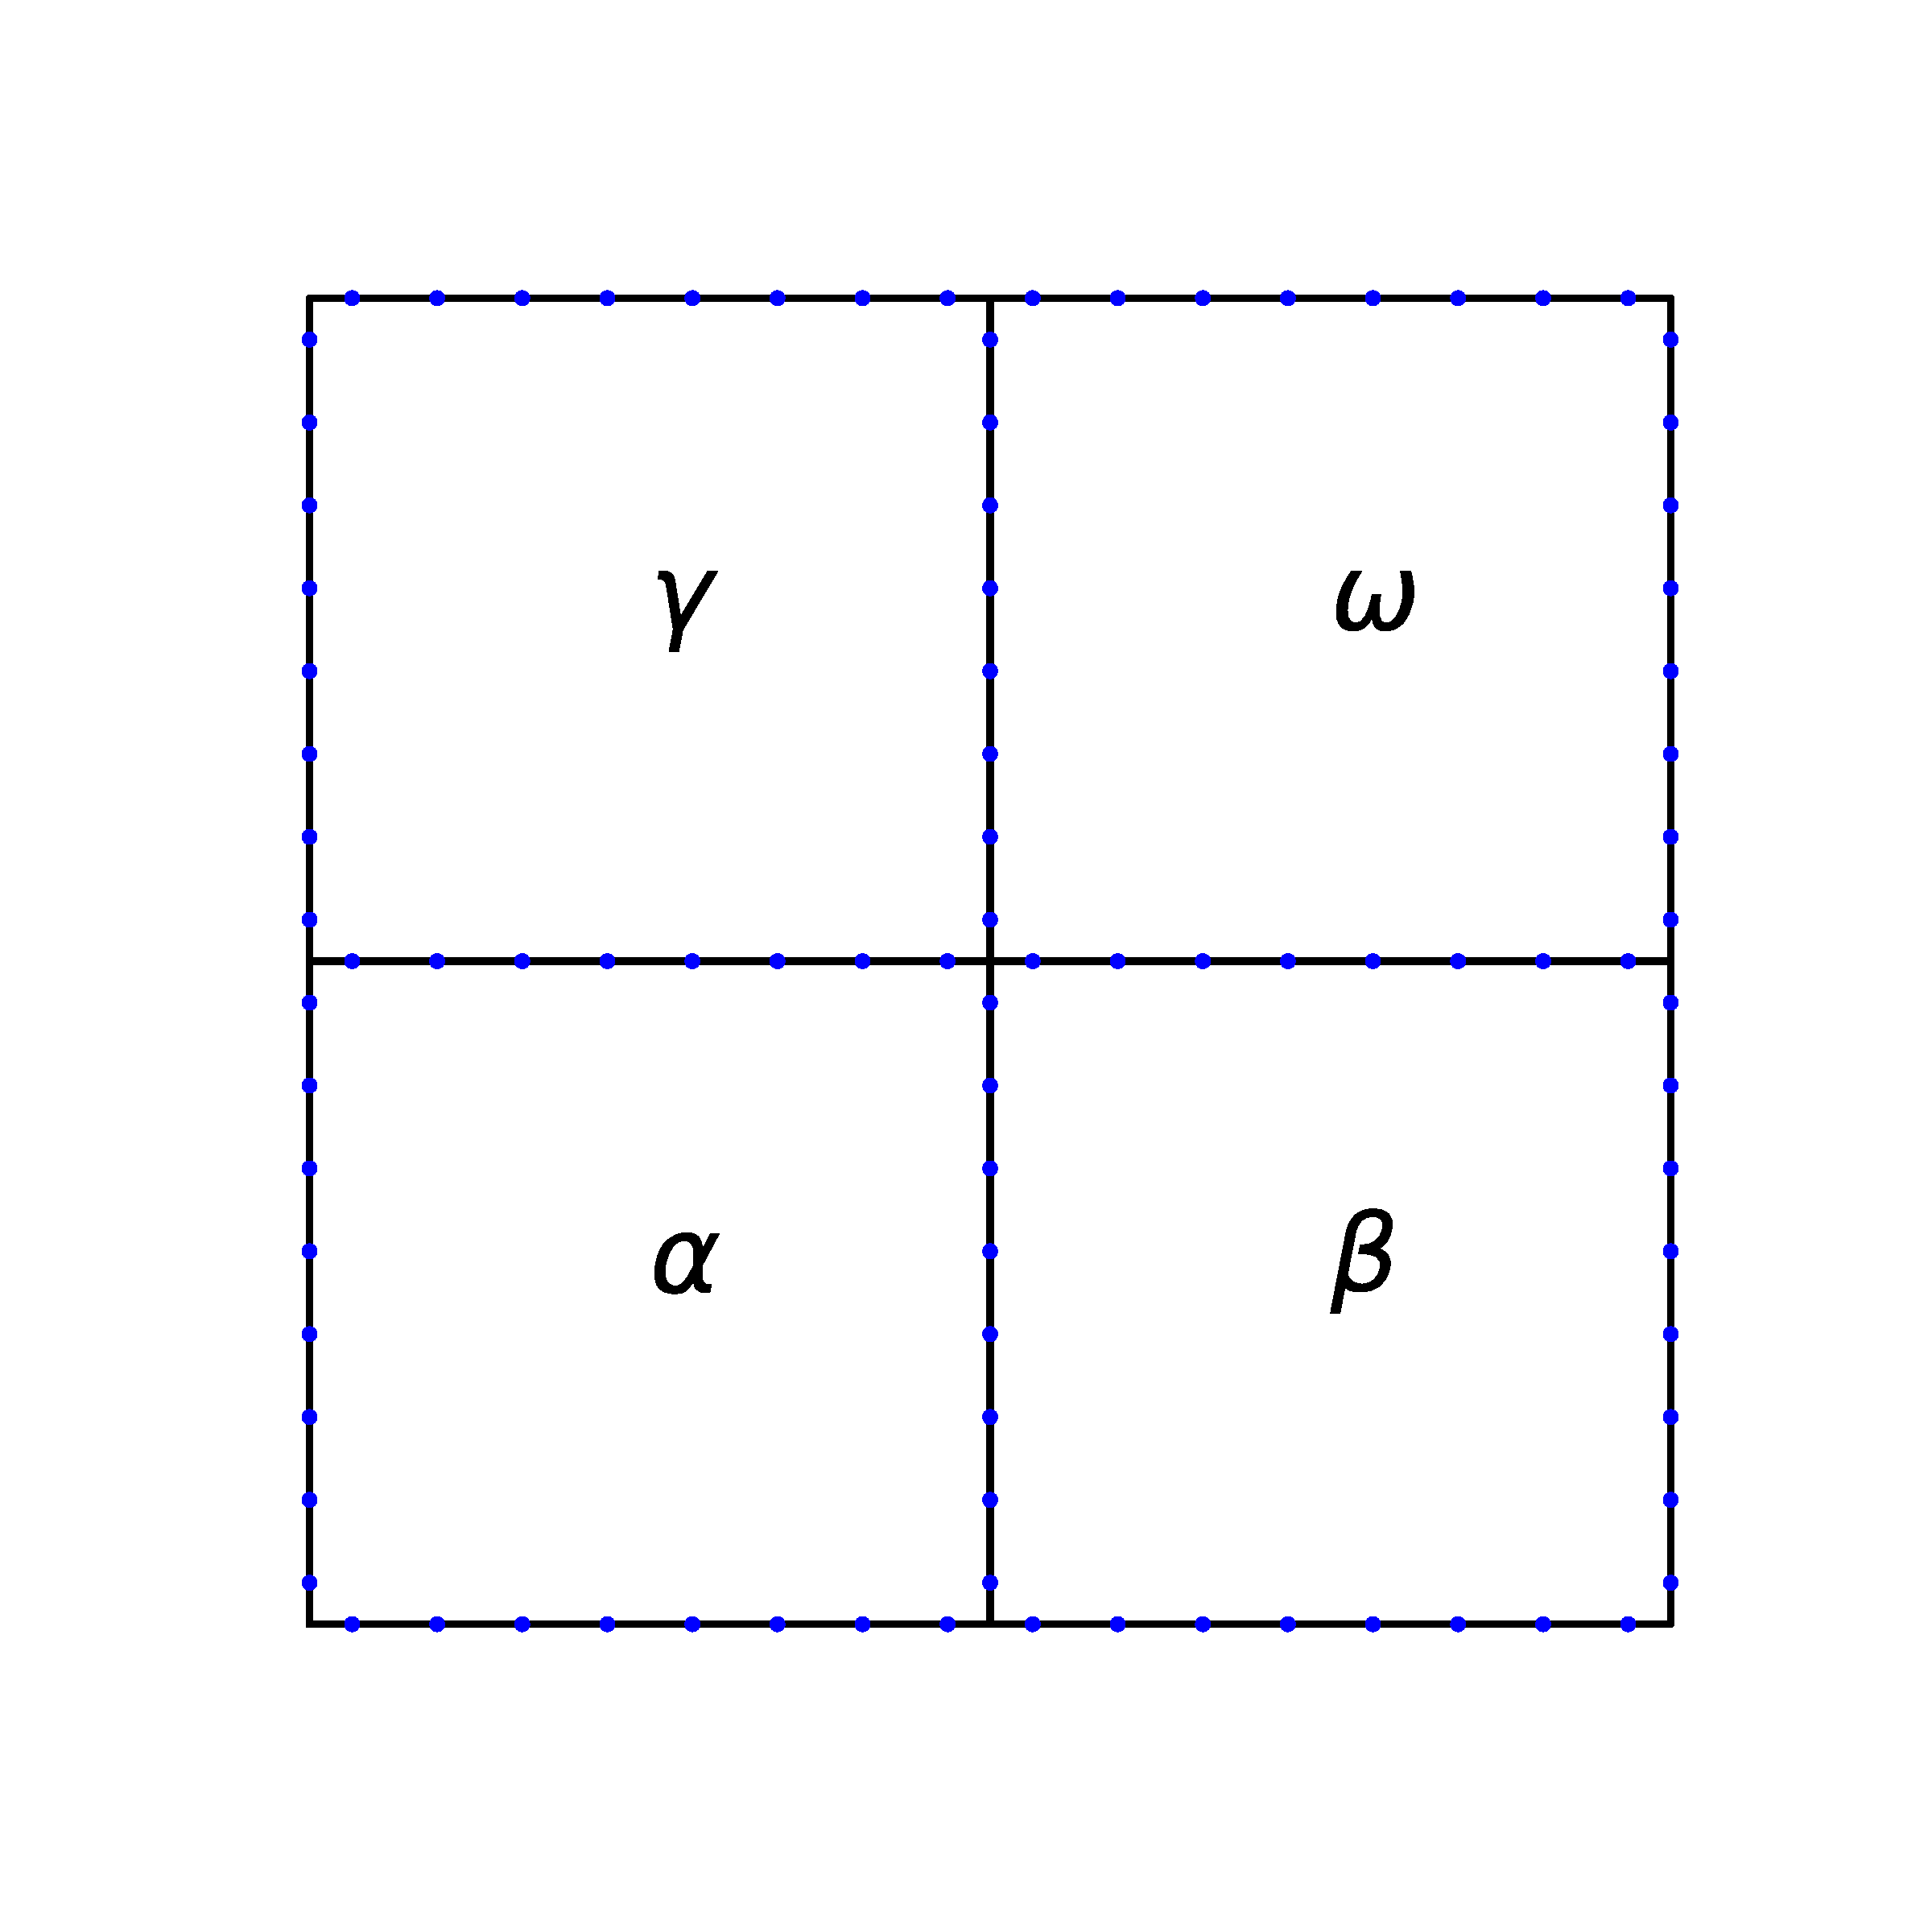
\includegraphics[width=\textwidth, clip=true, trim={100 150 100 150}]{figures/four_patches_without_points.pdf}
            \label{subfig:4_patches}
        \end{subfigure}
        &
        \begin{subfigure}[t]{0.3\textwidth}
            \centering
            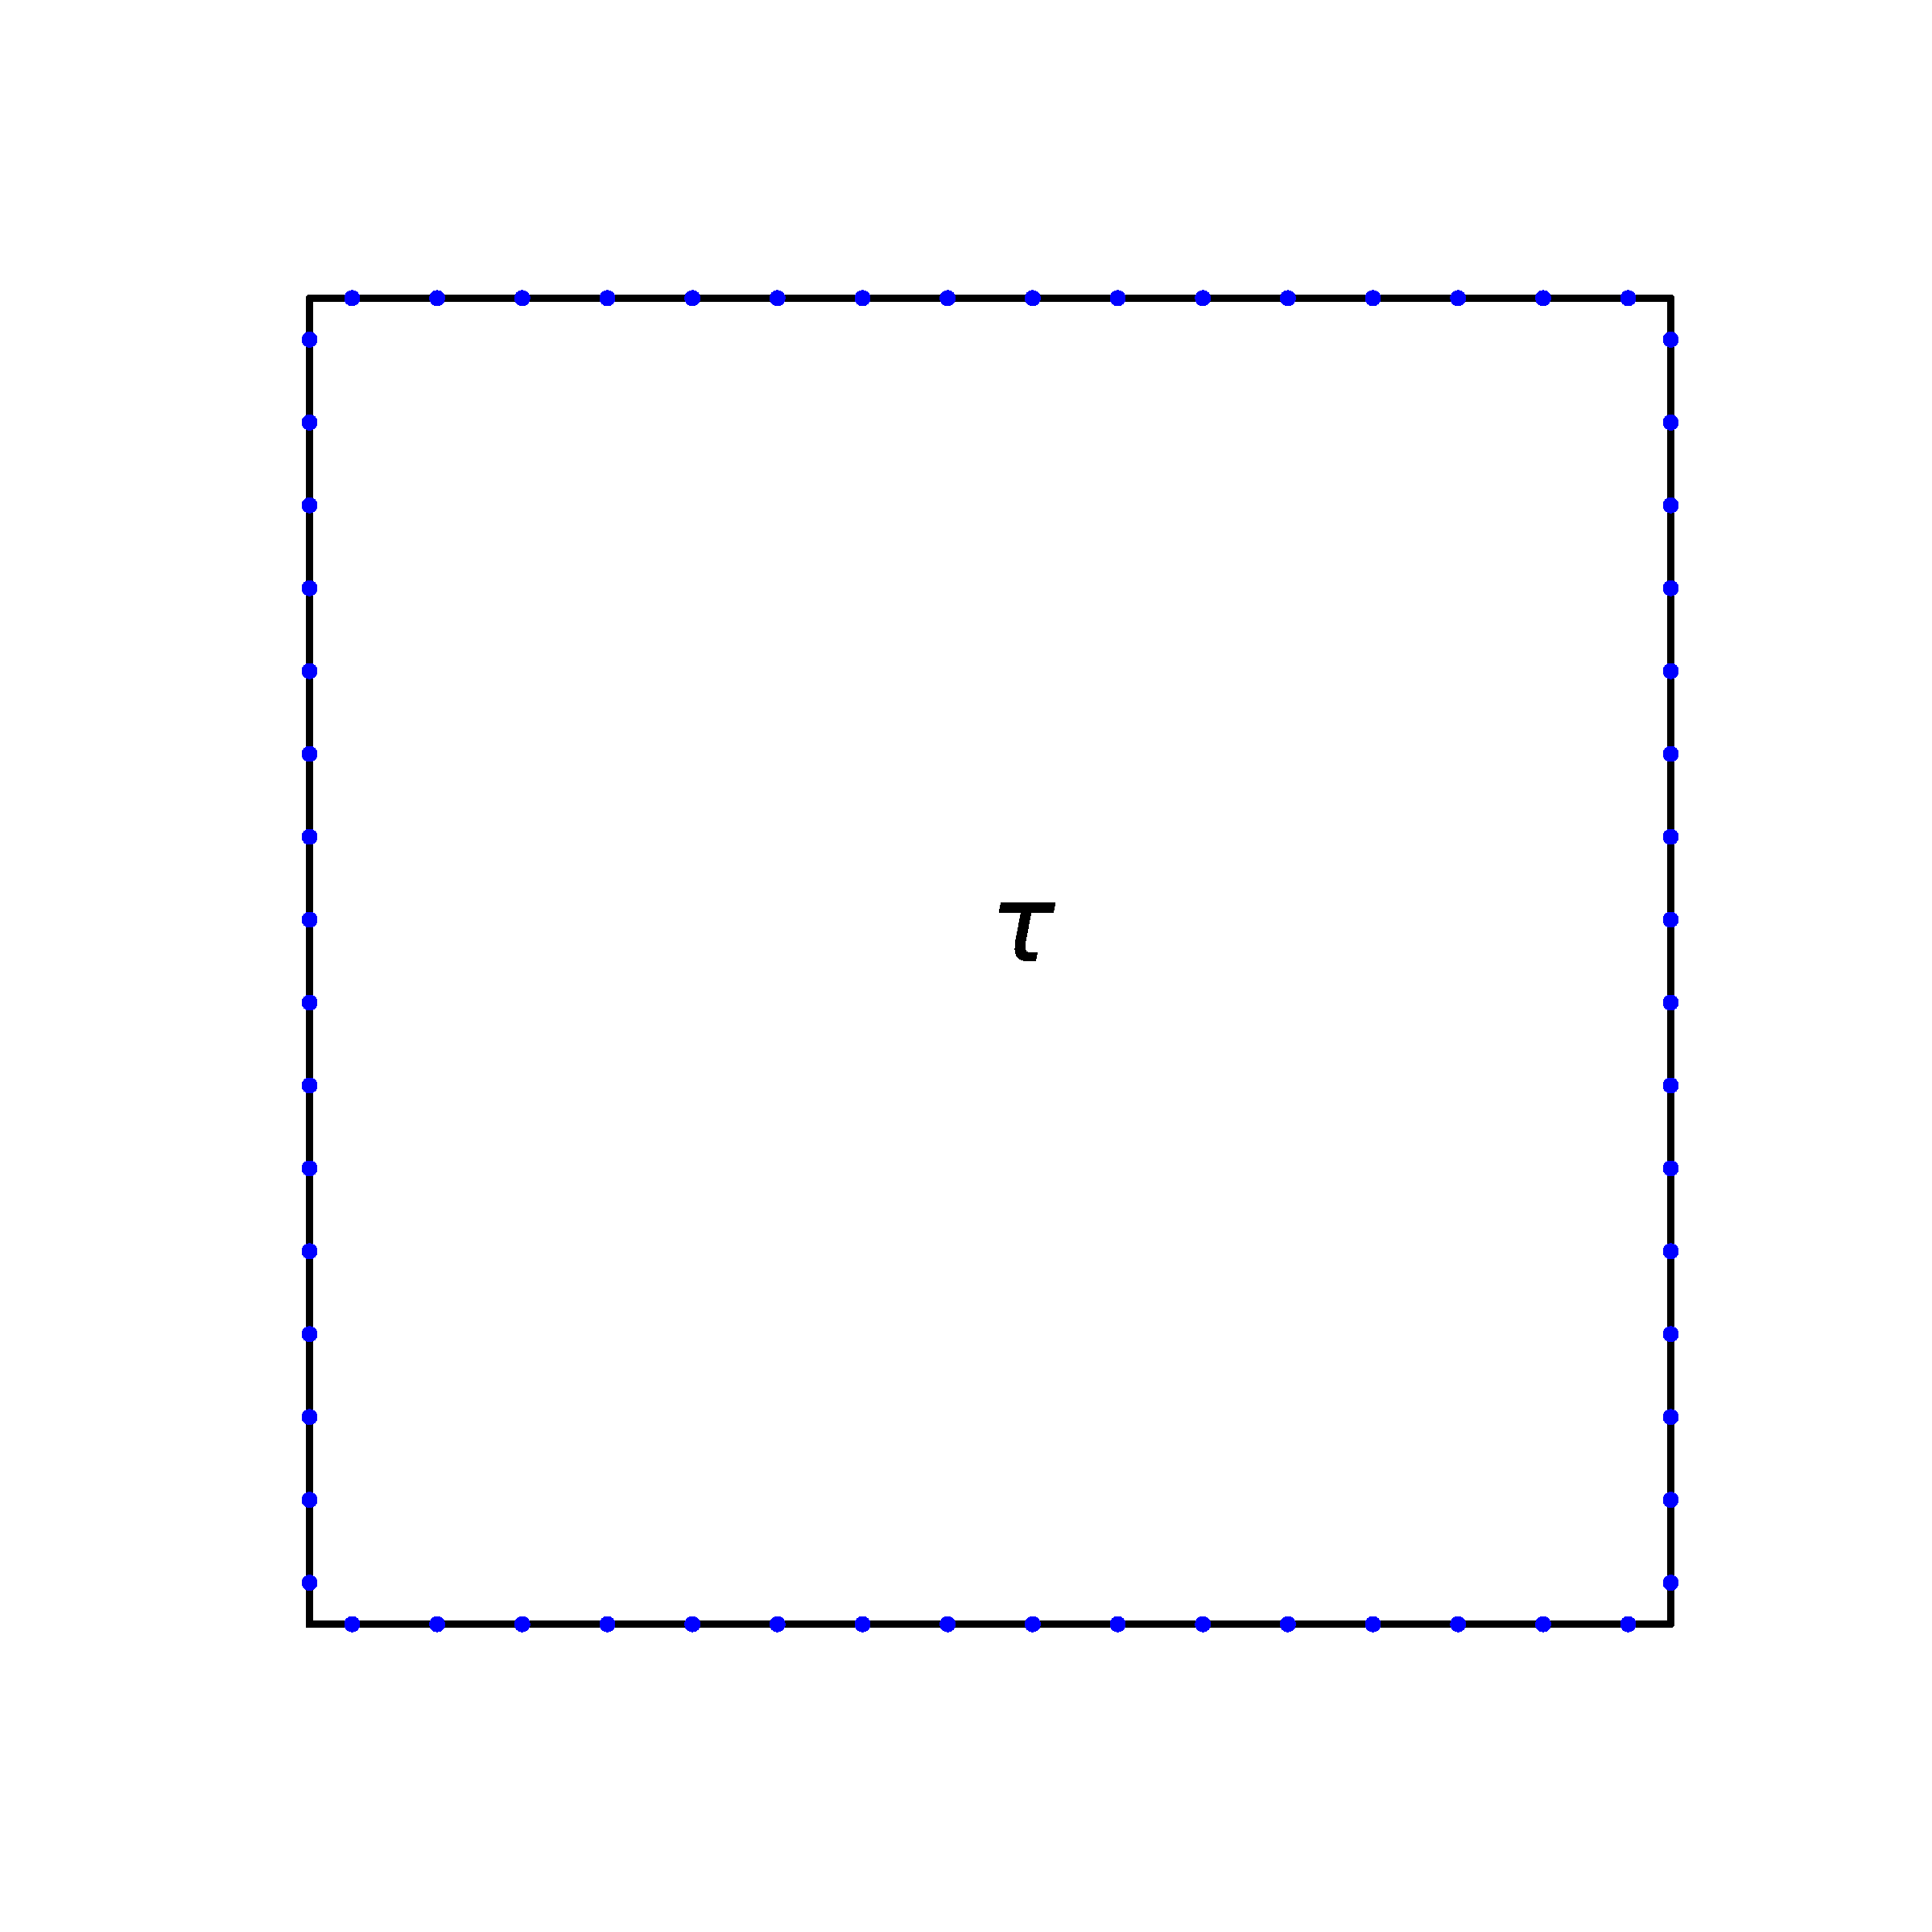
\includegraphics[width=\textwidth, clip=true, trim={100 150 100 150}]{figures/merged_patch.pdf}
            \label{subfig:parent_patch}
        \end{subfigure}
    \end{tabular}
    \caption{The 4-to-1 merge process: (left) the four children patches with their local grid, (middle) the four children share internal and external boundaries with $\tau$, (right) the merged parent patch with data on the exterior of $\tau$.}
    \label{fig:4_to_1_patches}
\end{figure}

% \begin{figure}
%     \centering
%     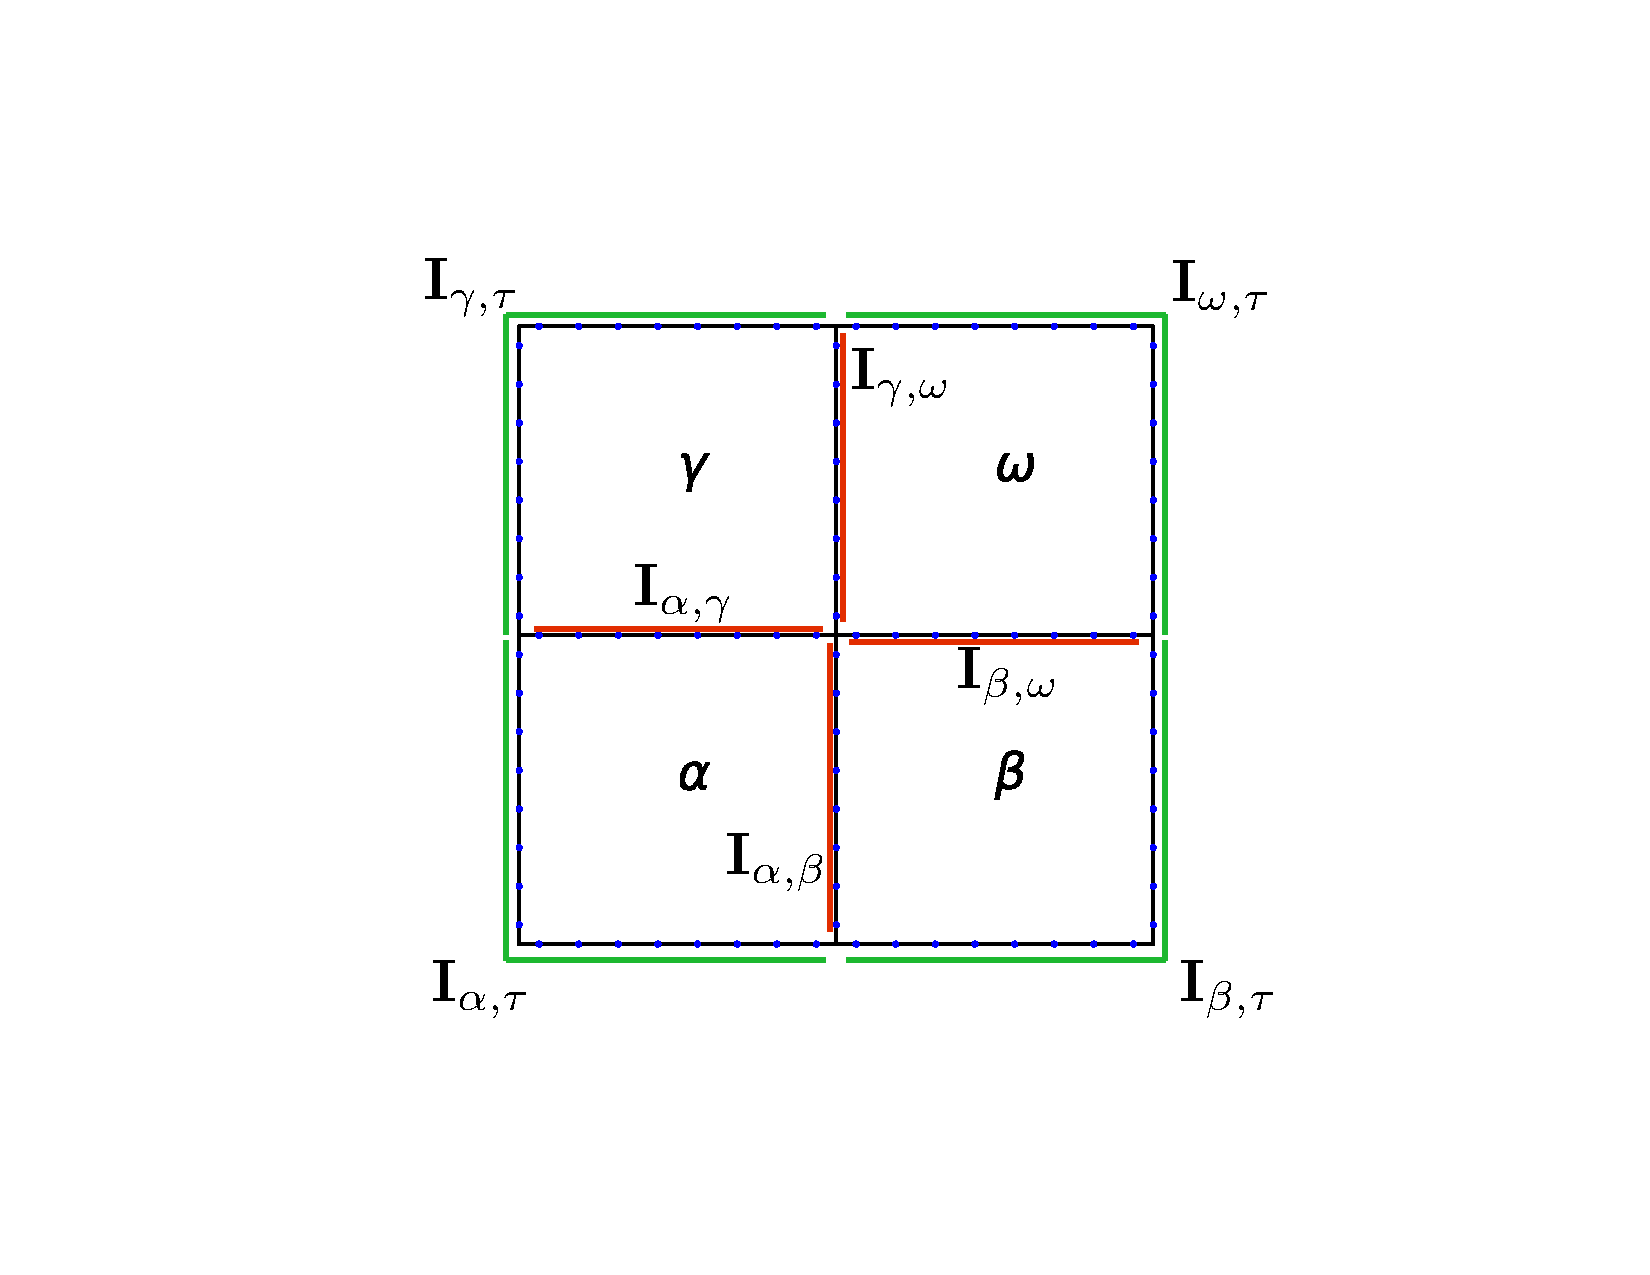
\includegraphics[width=0.5\textwidth]{figures/merging_index_sets.pdf}
%     \caption{An overview of the index sets used in the 4-to-1 merge. The index sets marked with green correspond to the exterior of $\tau$ and the index sets marked with red correspond to the interior of $\tau$.}
%     \label{fig:merged_index_sets}
% \end{figure}

\subsubsection{Merging DtN mappings} We partition sibling operators \Ti, $i=\alpha$, $\beta$, $\gamma$, $\omega$ according to how Dirichlet data on an edge of patch $i$ are mapped to an edge on $i$ containing Neumann data.  For example, the sub-matrix $\Talphap{\tau}{\gamma}$ maps Dirichlet data on the boundary shared between sibling patch $\alpha$  and parent patch $\tau$ to Neumann data on the boundary shared between patch $\alpha$ and sibling patch $\gamma$. In a similar manner, the Dirichlet data on each of the sibling patches $i$ into $\galphap{\tau}$, $\galphap{\gamma}$ and $\galphap{\beta}$, where the subscripts indicate data on edges that patch $\alpha$ shares with patches $\tau$, $\gamma$ and $\beta$. Neumann data $\valpha$ and \halpha are partitioned in an analogous manner. 

With these partitions, we can write a set of equations for each of the four sibling DtN mappings as
\begin{equation}
\begin{aligned}
\valpha = \Talpha \galpha + \halpha \quad & \Longrightarrow  & \quad 
    \begin{bmatrix}
    \valphap{\tau} \\
    \valphap{\gamma} \\
    \valphap{\beta} \\
    \end{bmatrix}
    =
    \begin{bmatrix}
    \Talphap{\tau}{\tau}   &\Talphap{\gamma}{\tau}   & \Talphap{\beta}{\tau} \\
    \Talphap{\tau}{\gamma} &\Talphap{\gamma}{\gamma} & \Talphap{\beta}{\gamma} \\
    \Talphap{\tau}{\beta}  &\Talphap{\gamma}{\beta}  & \Talphap{\beta}{\beta} \\
    \end{bmatrix}
    \begin{bmatrix}
    \galphap{\tau} \\
    \galphap{\gamma} \\
    \galphap{\beta} \\
    \end{bmatrix} + 
    \begin{bmatrix}
    \halphap{\tau} \\
    \halphap{\gamma} \\
    \halphap{\beta} \\
    \end{bmatrix}\\
&& \\
\vbeta = \Tbeta \gbeta + \hbeta \quad & \Longrightarrow  & \quad
    \begin{bmatrix}
        \vbetap{\tau} \\
        \vbetap{\omega} \\
        \vbetap{\alpha} \\
    \end{bmatrix}
    =
    \begin{bmatrix}
        \Tbetap{\tau}{\tau}   & \Tbetap{\omega}{\tau}   & \Tbetap{\alpha}{\tau} \\
        \Tbetap{\tau}{\omega} & \Tbetap{\omega}{\omega} & \Tbetap{\alpha}{\omega} \\
        \Tbetap{\tau}{\alpha} & \Tbetap{\omega}{\alpha} & \Tbetap{\alpha}{\alpha} \\
    \end{bmatrix}
    \begin{bmatrix}
        \gbetap{\tau} \\
        \gbetap{\omega} \\
        \gbetap{\alpha} \\
    \end{bmatrix} + 
    \begin{bmatrix}
        \hbetap{\tau} \\
        \hbetap{\omega} \\
        \hbetap{\alpha}
    \end{bmatrix}\\
&& \\
\vgamma = \Tgamma \ggamma + \hgamma \quad & \Longrightarrow  & \quad
    \begin{bmatrix}
        \vgammap{\tau} \\
        \vgammap{\alpha} \\
        \vgammap{\omega} \\
    \end{bmatrix}
    =
    \begin{bmatrix}
        \Tgammap{\tau}{\tau}    & \Tgammap{\alpha}{\tau}   & \Tgammap{\omega}{\tau} \\
        \Tgammap{\tau}{\alpha}  & \Tgammap{\alpha}{\alpha} & \Tgammap{\omega}{\alpha} \\
        \Tgammap{\tau}{\omega}  & \Tgammap{\alpha}{\omega} & \Tgammap{\omega}{\omega} \\
    \end{bmatrix}
    \begin{bmatrix}
        \ggammap{\tau} \\
        \ggammap{\alpha} \\
        \ggammap{\omega} \\
    \end{bmatrix} + 
    \begin{bmatrix}
        \hgammap{\tau} \\
        \hgammap{\alpha} \\
        \hgammap{\omega} \\
    \end{bmatrix}\\    
&& \\    
\vomega = \Tomega \gomega + \homega \quad & \Longrightarrow  & \quad
    \begin{bmatrix}
        \vomegap{\tau} \\
        \vomegap{\beta} \\
        \vomegap{\gamma} \\
    \end{bmatrix}
    =
    \begin{bmatrix}
        \Tomegap{\tau}{\tau}   & \Tomegap{\beta}{\tau}   & \Tomegap{\gamma}{\tau} \\
        \Tomegap{\tau}{\beta}  & \Tomegap{\beta}{\beta}  & \Tomegap{\gamma}{\beta} \\
        \Tomegap{\tau}{\gamma} & \Tomegap{\beta}{\gamma} & \Tomegap{\gamma}{\gamma} \\
    \end{bmatrix}
    \begin{bmatrix}
        \gomegap{\tau} \\
        \gomegap{\beta} \\
        \gomegap{\gamma} \\
    \end{bmatrix} +
    \begin{bmatrix}
        \gomegap{\tau} \\
        \gomegap{\beta} \\
        \gomegap{\gamma} \\
    \end{bmatrix} \\
\end{aligned}.
\label{eq:linalg_one}
\end{equation}
Taking the first equation from each of the four sets of equations in \eqn{linalg_one}, we write a system of equations for the Dirichlet data to get
\begin{equation}
A\gext + B \gint + \hext = \vext
\label{eq:sys_one}
\end{equation}
where the Dirichlet data has been partitioned into {\em exterior} data and {\em interior} data.  The exterior data is data on the boundary of the parent patch $\tau$ is given by
\begin{equation}
\gext \equiv \left[\galphap{\tau}, \gbetap{\tau} , \ggammap{\tau}, \gomegap{\tau}\right]^T
\end{equation}
To define the interior data, we use the fact that our solution is continuous across boundaries shared by sibling grids and enumerate data on the four shared boundaries as
\begin{equation}
\begin{aligned}
\gzero \equiv \galphap{\gamma} & = \ggammap{\alpha}\\
\gone \equiv \gbetap{\omega} & = \gomegap{\beta}  \\
\gtwo \equiv \galphap{\beta} & = \gbetap{\alpha} \\
\gthree \equiv \ggammap{\omega} & = \gomegap{\gamma}.
\end{aligned}
\end{equation}
With the Dirichlet data on the shared boundary uniquely defined, the interior partition of the Dirichlet data is given as
\begin{equation}
\gint \equiv \left[\gzero, \gone, \gtwo, \gthree\right]^T
\end{equation}
The Neumann data \vtau and \htau is partitioned analogously. 

The block matrices $A$ and $B$ are defined as
\begin{equation}
A = \begin{bmatrix}
\Talphap{\tau}{\tau} & \zeromat & \zeromat & \zeromat \\
\zeromat & \Tbetap{\tau}{\tau} & \zeromat & \zeromat  \\
\zeromat & \zeromat & \Tgammap{\tau}{\tau} & \zeromat  \\
\zeromat& \zeromat & \zeromat & \Tomegap{\tau}{\tau} \\
\end{bmatrix}, \qquad
B = \begin{bmatrix}
\Talphap{\gamma}{\tau} & \zeromat              & \Talphap{\beta}{\tau} & \zeromat \\
\zeromat               & \Tbetap{\omega}{\tau} & \Tbetap{\alpha}{\tau} & \zeromat \\
\Tgammap{\alpha}{\tau} & \zeromat              & \zeromat              & \Tgammap{\omega}{\tau} \\
\zeromat               & \Tomegap{\beta}{\tau} & \zeromat              & \Tomegap{\gamma}{\tau}
\end{bmatrix}
\label{eq:matrix_AB}
\end{equation}

To obtain a second set of equations, we impose a continuity condition on the normal derivative across edges shared between sibling patches and get
\begin{equation}
\begin{aligned}
\valphap{\gamma} + \vgammap{\alpha} & = \zeromat \\
\vbetap{\omega} + \vomegap{\beta} & = \zeromat \\
\valphap{\beta}  + \vbetap{\alpha} & = \zeromat\\
\vgammap{\omega} + \vomegap{\gamma} & = \zeromat.
\end{aligned}
\end{equation}
We organize the resulting four equations as
\begin{equation}
C \gext + D\gint  + \Deltah = \zeromat
\label{eq:sys_two}
\end{equation}
where
\begin{equation}
C = 
\begin{bmatrix}
\Talphap{\tau}{\gamma} & \zeromat               & \Tgammap{\tau}{\alpha} & \zeromat \\
\zeromat               & \Tbetap{\tau}{\omega}  & \zeromat                & \Tomegap{\tau}{\beta} \\ 
\Talphap{\tau}{\beta}  & \Tbetap{\tau}{\alpha} & \zeromat                & \zeromat \\
\zeromat               & \zeromat               & \Tgammap{\tau}{\omega}  & \Tomegap{\tau}{\gamma},
\end{bmatrix}
\end{equation}
\begin{equation}
D = \begin{bmatrix}
\Talphap{\gamma}{\gamma} + \Tgammap{\alpha}{\alpha} 
& \zeromat 
& \Talphap{\beta}{\gamma} 
& \Tgammap{\omega}{\alpha} \\
% 
\zeromat 
& \Tbetap{\omega}{\omega} + \Tomegap{\beta}{\beta} 
& \Tbetap{\alpha}{\omega} 
& \Tomegap{\gamma}{\beta} \\
% 
\Talphap{\gamma}{\beta} 
& \Tbetap{\omega}{\alpha} 
& \Talphap{\beta}{\beta}+ \Tbetap{\alpha}{\alpha} 
& \zeromat \\
% 
\Tgammap{\alpha}{\omega} 
& \Tomegap{\beta}{\gamma} 
& \zeromat 
& \Tgammap{\omega}{\omega} + \Tomegap{\gamma}{\gamma}
\end{bmatrix}
\label{eq:matrix_CD}.
\end{equation}
and 
\begin{equation}
\Deltah = 
\begin{bmatrix}
\halphap{\gamma} + \hgammap{\alpha} \\
\hbetap{\omega} + \homegap{\beta} \\
\halphap{\beta} + \hbetap{\alpha} \\
\hgammap{\omega} + \homegap{\gamma}
\end{bmatrix}.
\end{equation}

Combining \eqn{sys_one} and \eqn{sys_two}, we have
\begin{equation}
\begin{aligned}
A\gext + B\gint + \hext & = \vext \\
C\gext + D\gint + \Deltah & = \zeromat
\end{aligned}
\end{equation}
Writing this system as an augmented system and applying a single step of block Gaussian elimination, we get
\begin{equation}
\left[
\begin{array}{cc|c}
A & B & \vext - \hext\\
C & D & -\Deltah\\
\end{array}\right]
\;
\Longrightarrow 
\;
\left[
\begin{array}{cc|c}
A - BD^{-1}C & 0 & \vext - \hext + B D^{-1}\Deltah\\
D^{-1}C      & I & -D^{-1}\Deltah
\end{array}\right]
\label{eq:reduced_system}
\end{equation}
We express the first row of the reduced system in equation form as 
\begin{equation}
\left(A - BD^{-1}C\right) \gext = \vext - \hext + B D^{-1}\Deltah
\label{eq:complete_ops}
\end{equation}
From this, we can identify the {\em merged} DtN operator 
\begin{equation}
\Ttau \equiv \mathbf{A} - \mathbf{B} \mathbf{D}^{-1} \mathbf{C} 
\label{eq:Ttau-merged}
\end{equation}
as the operator that maps exterior Dirichlet data to exterior Neumann data, with merged inhomogeneous Neumann data given as
\begin{equation}
\htau \equiv -\hext + B D^{-1}\Deltah. 
\label{eq:htau-merged}
\end{equation}
With these choices of \Ttau and \htau  we recover the expression from \eqn{vtau}.

The second row of the reduced system \eqn{reduced_system}, given by 
\begin{equation}
\gint = -D^{-1}C \gext -D^{-1} \Deltah,
\end{equation}
shows us how to recover interior Dirichlet data \gint  from exterior data \gext.  
From this, we introduce the {\em solve} operator \Stau, given by 
\begin{equation}
\Stau \equiv -D^{-1}C
\label{eq:Stau-merged}
\end{equation}

Introducing  the operator
\begin{equation}
\Xtau \equiv -D^{-1}
\label{eq:xtau}
\end{equation}
we can write \Ttau and  \Stau in convenient form as
\begin{equation}
\begin{aligned}
\Stau & = \Xtau C \\
\Ttau & = A + B\Stau \\
\label{eq:stau_ttau}
\end{aligned}
\end{equation}
To compute the merged inhomogeneous term, we first compute
\begin{equation}
\wtau \equiv \Xtau\Deltah
\label{eq:wtau-merged}
\end{equation}
so that
\begin{equation}
\htau = -\hext - B\wtau
\label{eq:htau}
\end{equation}

Once the build stage is complete, the solve state maps Dirichlet data on parent quadrants to Dirichlet data on child quadrants via the solve operator \Stau, as
\begin{equation}
\gint = \Stau \gext + \wtau.
\label{eq:solve_eqn}
\end{equation}

The formalism presented in terms of merged components \Xtau, \Stau, \Ttau and \htau is identical to that presented in \citep{martinsson2015hierarchical} for the horizontal merge of two leaf boxes.

The build stage of HPS method is described in \Alg{build_merge_uniform}
\begin{algorithm}[H]
    \caption{Build stage on a uniformly refined quadtree mesh}
    \begin{algorithmic}[0]
        \For{$\tau = 0,1,\dots$} \Comment{Iterate over quadrants in uniform quadtree}
            \If{$\tau$ is a leaf-level patch}
                \State Build and store leaf-level DtN map \Ttau and inhomogeneous data \htau
            \Else \Comment{$\tau$ has four child patches $i$, $i=\alpha$, $\beta$, $\gamma$, $\omega$.}
                \State Solve $D\Stau = -C$ to get operator \Stau. 
                \State Build operator \Ttau using \eqn{stau_ttau}.      
                \State Solve $D\wtau = \Deltah$ using to get \wtau.  
                \State Build merged inhomogeneous vector \htau using \eqn{htau}.
                \State Store \Stau, \Ttau, \htau and \wtau with quadrant $\tau$.
                \State Delete operators \Talpha, \Tbeta, \Tgamma, \Tomega and inhomogeneous data \halpha, \hbeta, \hgamma and \homega.
            \EndIf
        \EndFor
    \end{algorithmic}
    \label{alg:build_merge_uniform}
\end{algorithm}
At the end of this build stage, we will have a single DtN operator \Ttau and single vector \htau for the root patch.  At all levels, though, we will have a solve operator \Stau and inhomogeneous vector \wtau.

A solve stage of the HPS method starts with data $g(x,y)$ defined on the boundary of the domain and successively ``splits" the domain by mapping this exterior Dirichlet data to interior data.  At the leaf level, we solve the Poisson problem \eqn{patch_poisson_problem}.  The solve stage algorithm is described in \Alg{solve_uniform}.
\begin{algorithm}[H]
    \caption{Solve stage on a uniformly refined quadtree mesh}
    \begin{algorithmic}[0]
        \For{$\tau = N,N-1,\hdots,0$} \Comment{Iterate over quadrants in uniform quadtree}
            \If{$\tau$ is a leaf-level patch}
                \State Solve patch Poisson problem \eqn{patch_poisson_problem}
            \Else{} \Comment{$\tau$ has four child patches $\alpha$, $\beta$, $\gamma$, $\omega$.}
                \State Use \eqn{solve_eqn} to map Dirichlet \gext on $\tau$ to Dirichlet data \gint on the interior shared child patch boundaries.
            \EndIf
        \EndFor
    \end{algorithmic}
    \label{alg:solve_uniform}
\end{algorithm}

% \begin{remark}
%     If the HPS solver is to be used with multiple right hand-sides for the same composite quadtree mesh, the build stage as described above should be separated into a "factorization" stage that only stores the operators \Ttau and \Stau and a second "upwards" stage that builds the inhomogeneous data \wtau from \htau for each patch. If the problem in \eqn{elliptic-pde} has zero right-hand side data, any operations involving \htau can be eliminated, since the inhomogeneous Neumann data will be identically zero.
% \end{remark}

% \remark{For a constant coefficient problem on a uniformly refined mesh, only one operator \Ttau per level needs to be computed and stored. In merge stage, this single operator can be used in place of each child patch. This significantly reduces the time needed in the build stage.}

% \remark{Neumann boundary data $v_k$ supplied along any segment of the domain boundary in \eqn{elliptic-pde} can be easily converted to a Dirichlet data $g_k$ using the formula
% \begin{equation}
% g_k = \ukin + \frac{h}{2}v_k
% \end{equation}
% This Dirichlet data is then propagated down to the leaf-level patches using \Alg{solve_uniform}.}

\subsection{Coarse-Fine Interfaces}
\label{sub:mesh_adaptivity}

The merging and splitting processes we have described so far applies only to four sibling patches occupying a coarser level quadrant. For a fully adaptive quadtree, however, not all quadrants are refined to the same level, resulting in coarse-fine interfaces (see \reffig{fig:adaptive_merge}). To accommodate for the coarse-fine interfaces, we coarsen entire patches with coarse-fine interfaces. This approach is similar to the approach used in \citep{babb2018accelerated}. The mesh is not changed as a result of this process, just the data on a patch, as detailed below.

\begin{figure}
    \centering
    \begin{tabular}{ccc}
        \begin{subfigure}[t]{0.3\textwidth}
            \centering
            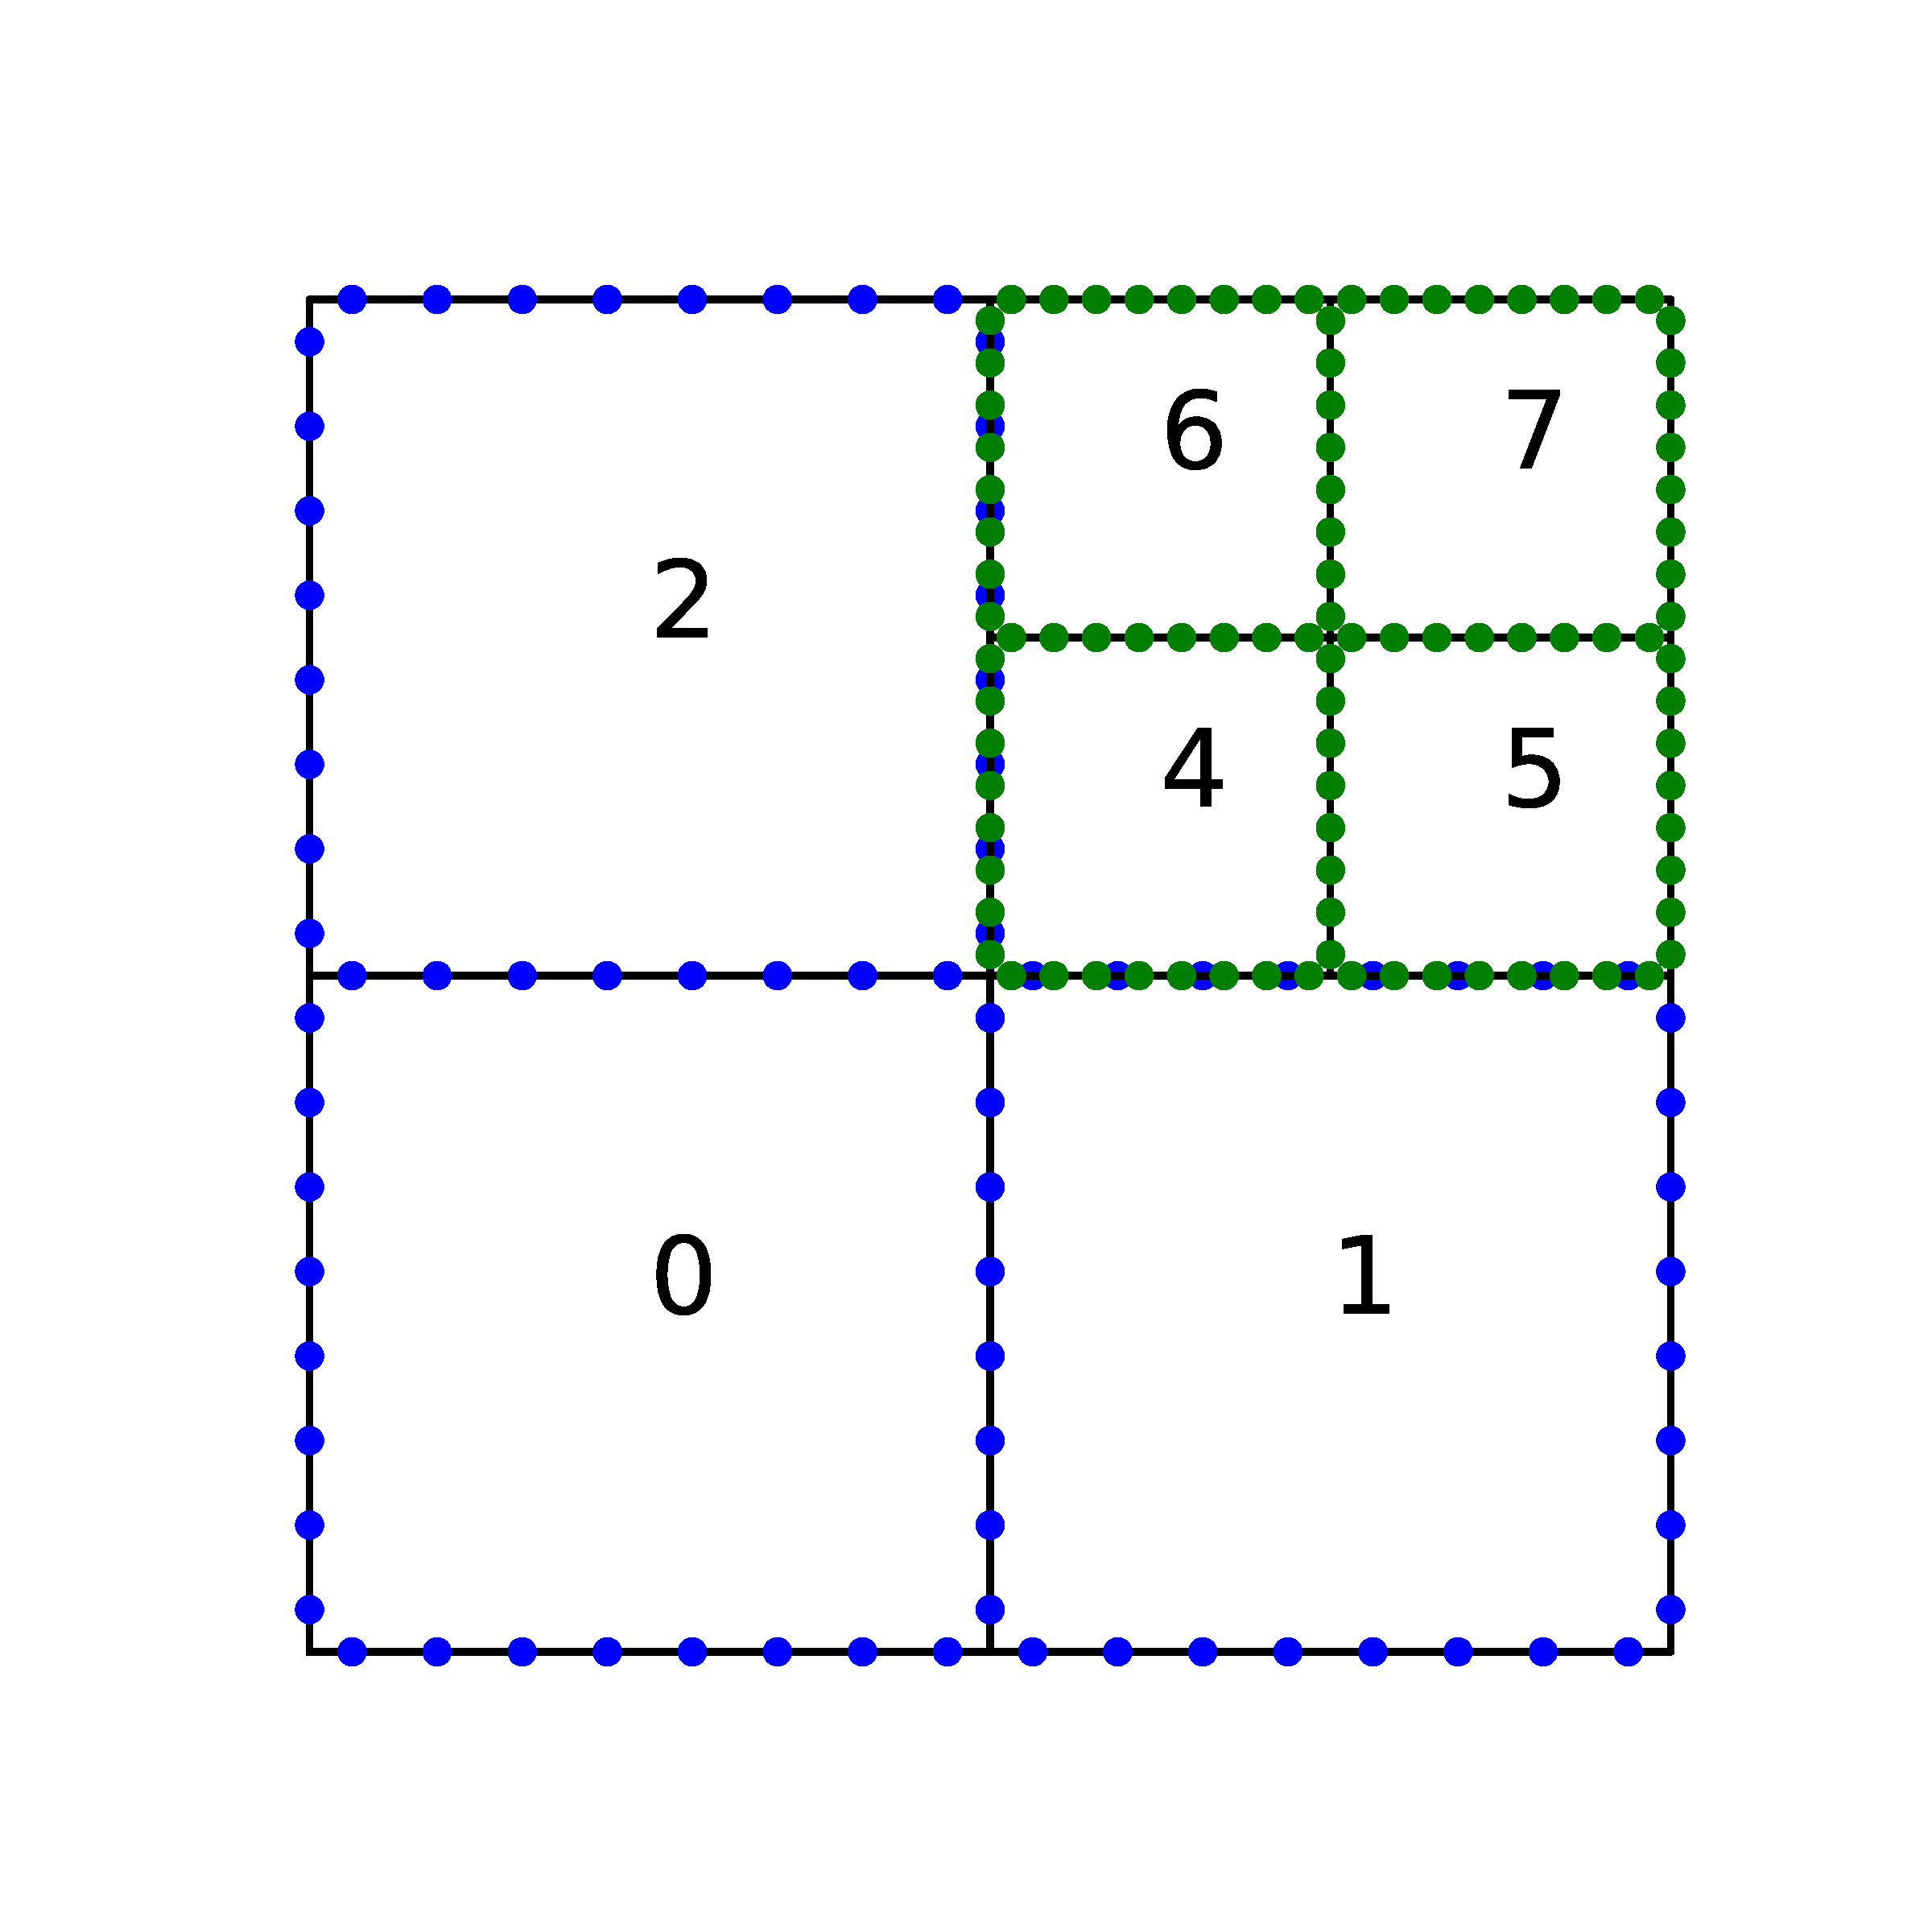
\includegraphics[width=\textwidth, clip=true, trim={100 150 100 150}]{figures/adaptive_merge1.pdf}
        \end{subfigure}
        &
        \begin{subfigure}[t]{0.3\textwidth}
            \centering
            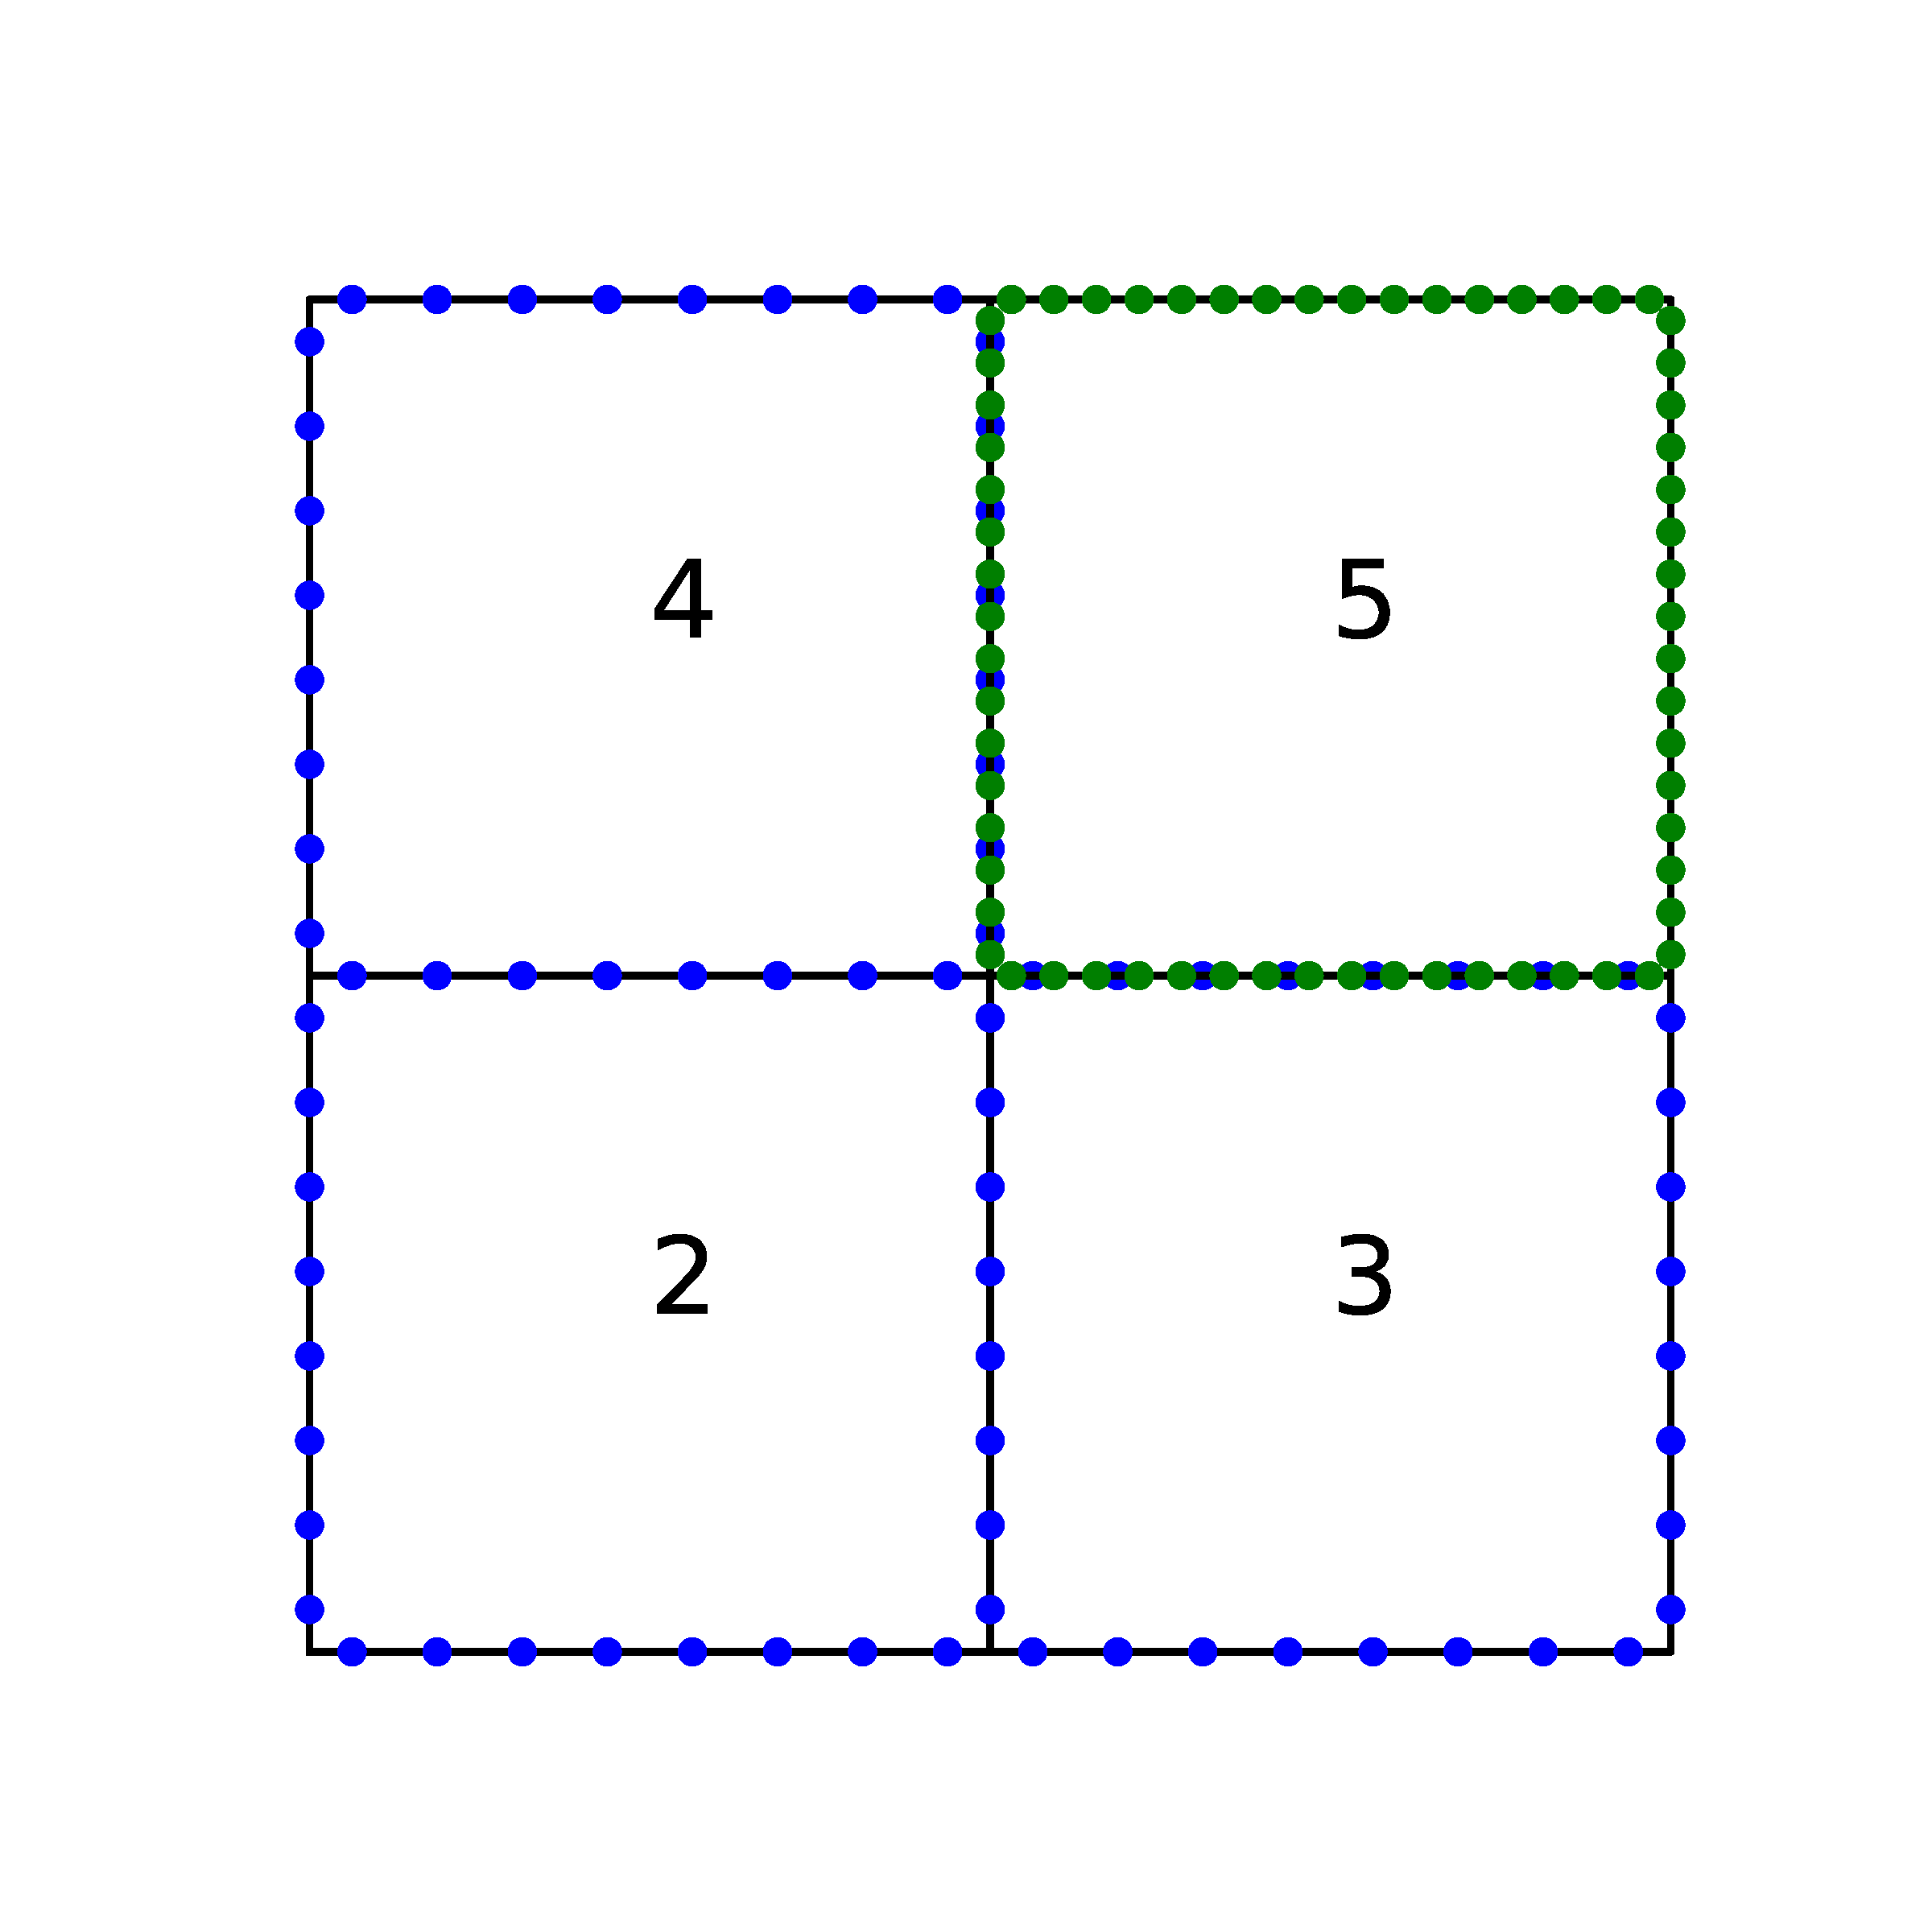
\includegraphics[width=\textwidth, clip=true, trim={100 150 100 150}]{figures/adaptive_merge2.pdf}
        \end{subfigure}
        &
        \begin{subfigure}[t]{0.3\textwidth}
            \centering
            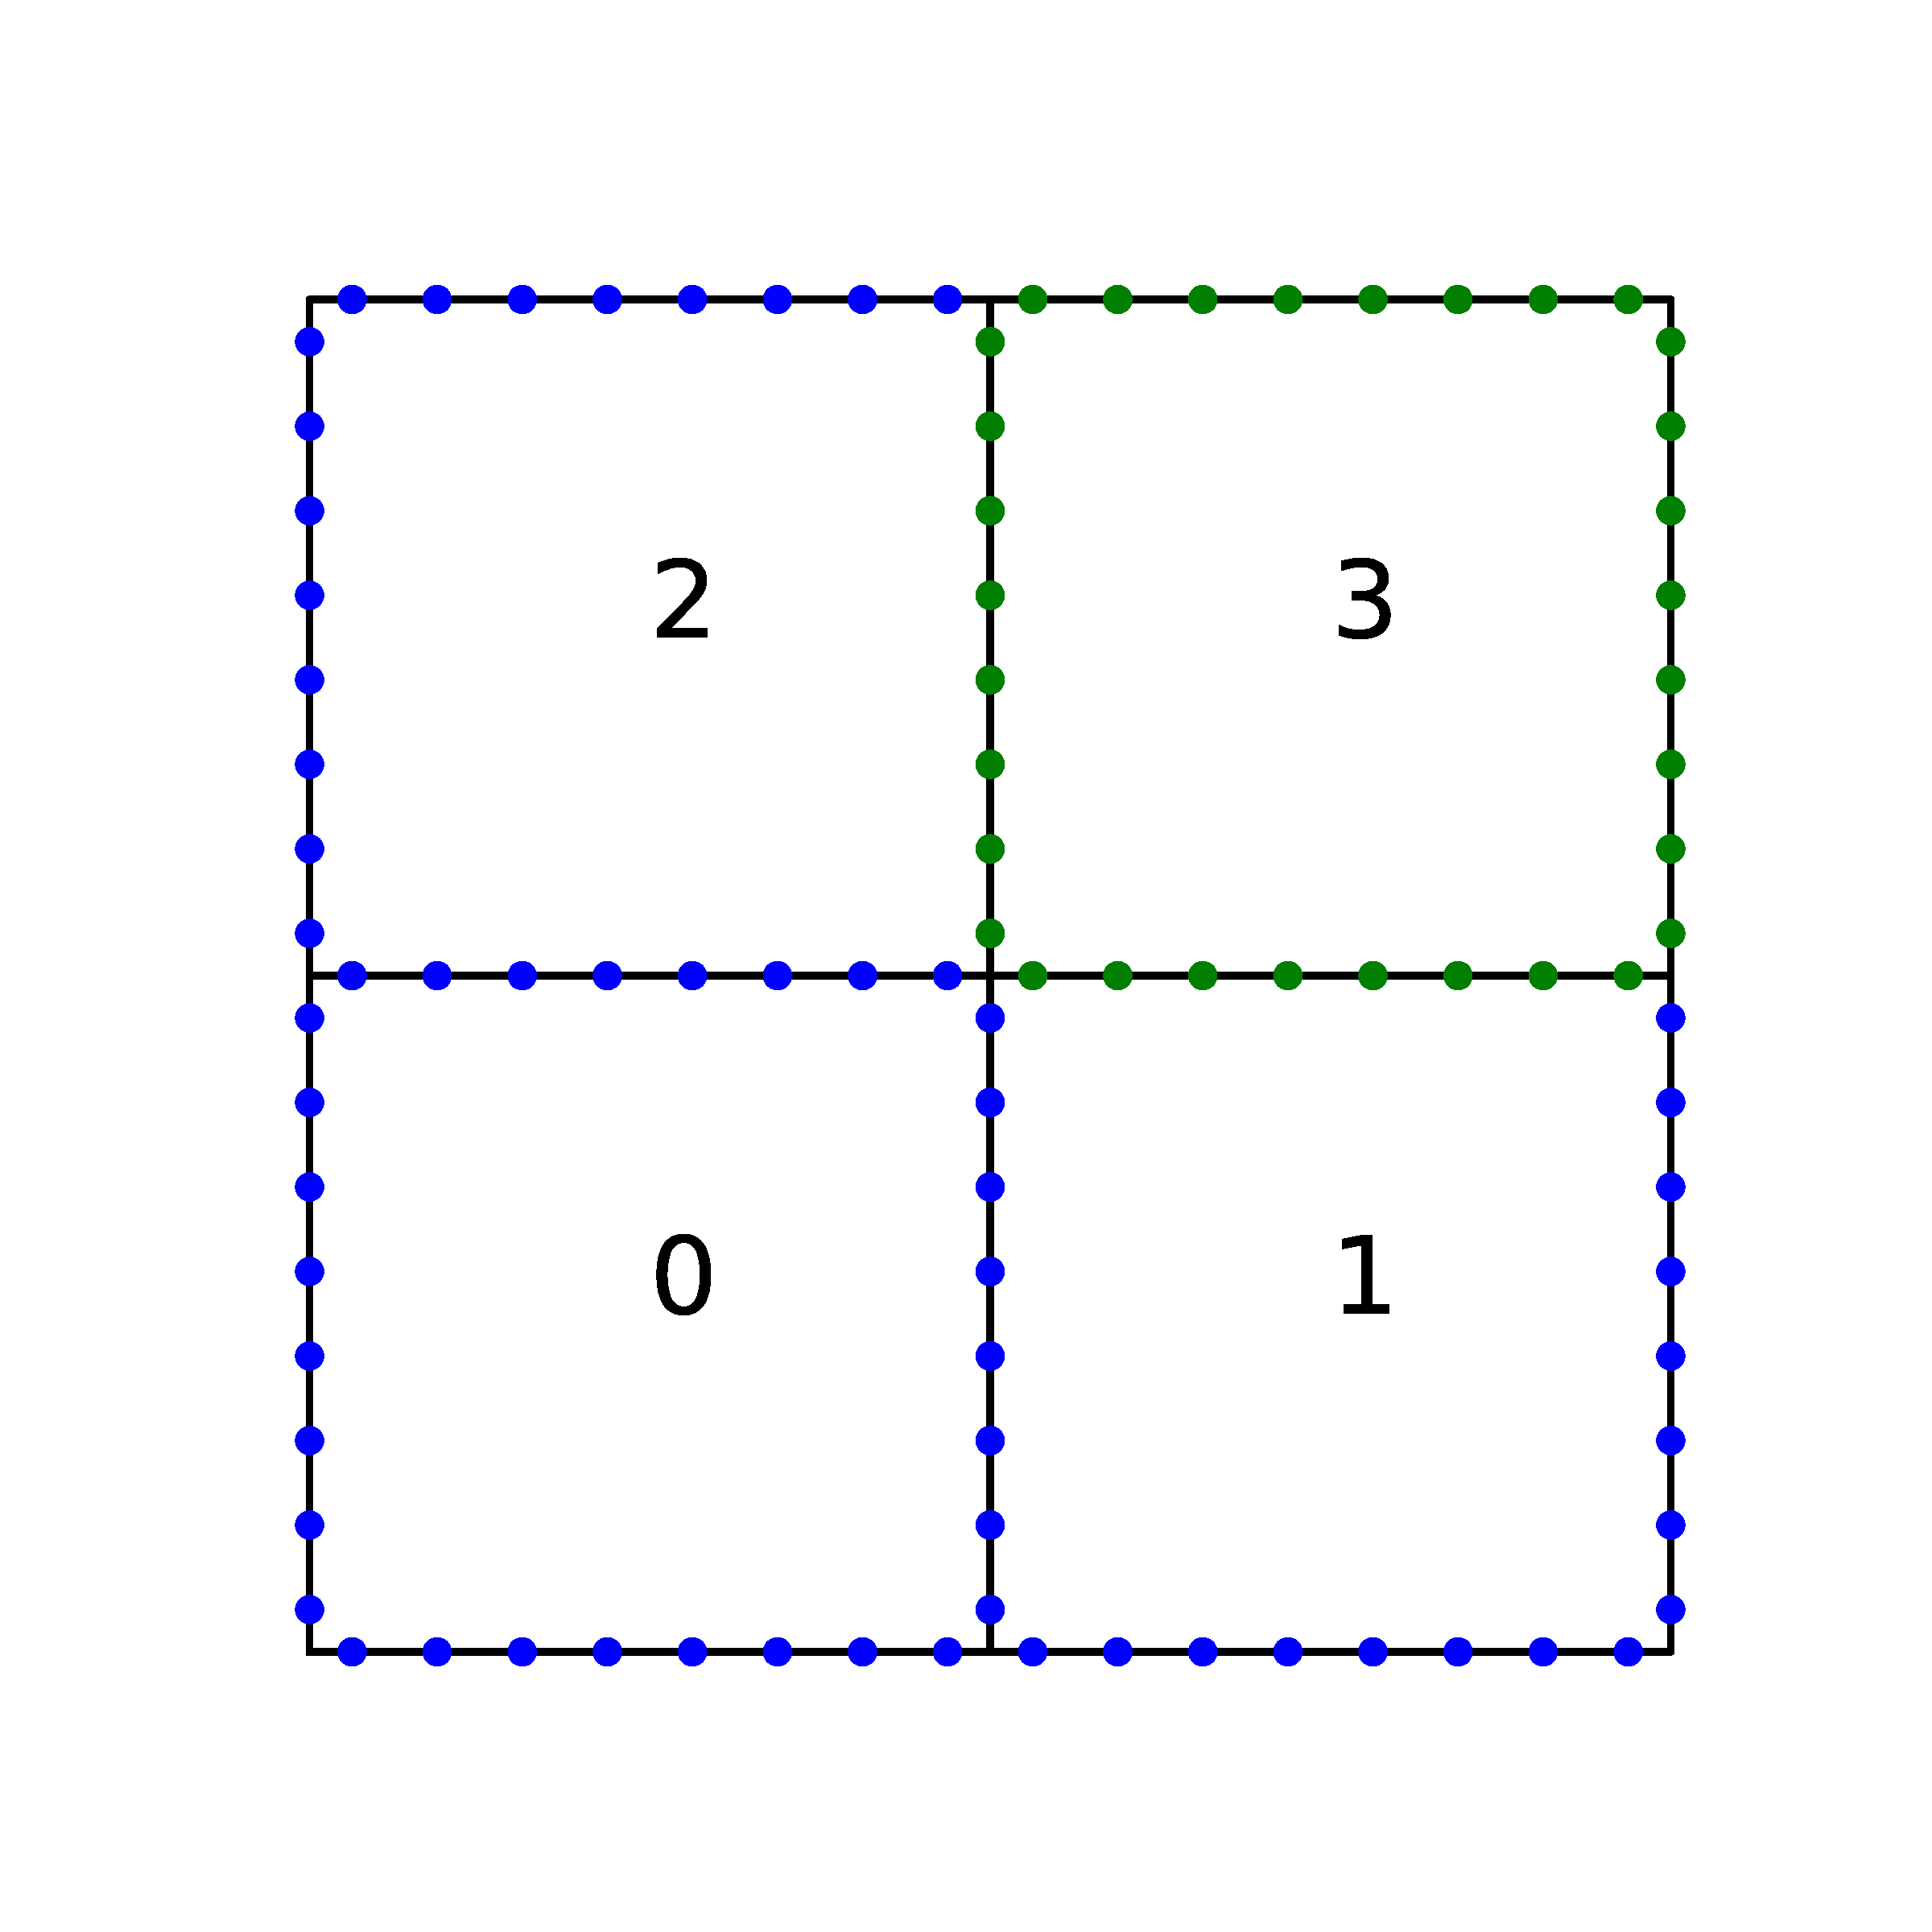
\includegraphics[width=\textwidth, clip=true, trim={100 150 100 150}]{figures/adaptive_merge3.pdf}
        \end{subfigure}
    \end{tabular}
    \caption{Example of a coarse-fine interface merge: (left) patches $6, 7, 8, \&\ 9$ will be merged and result in a coarse-fine interface, (middle) the data on patch 5 is averaged (coarsened), (right) merging $2, 3, 4, \&\ 5$ can continue as detailed in \refsec{sub:4-to-1merge}.}
    \label{fig:adaptive_merge}
\end{figure}

Prior to merging, we check each of the four children patches to be merged for a patch with data more fine than the other children. We do this by checking the size of the associated grid on that patch. If a coarse-fine interface exists, the data on that patch gets coarsened so as to match its siblings. For the build stage, only $\mathbf{T}^{\tau}$ and $\textbf{h}^{\tau}$ need to be coarsened. We form interpolation matrices $\textbf{L}_{2,1}$ and $\textbf{L}_{1,2}$ that map two sides to one or one side to two, respectively. As we employ a cell-centered grid, these matrices either average two data points to one, or interpolate one data point to two. Block diagonal versions of these are formed as
\begin{align}
    \textbf{L}_{2,1}^{B} &= \texttt{BlockDiag}(\{\textbf{L}_{2,1}, \textbf{L}_{2,1}, \textbf{L}_{2,1}, \textbf{L}_{2,1}\}) \\
    \textbf{L}_{1,2}^{B} &= \texttt{BlockDiag}(\{\textbf{L}_{1,2}, \textbf{L}_{1,2}, \textbf{L}_{1,2}, \textbf{L}_{1,2}\})
\end{align}
and coarsening $\textbf{T}$ and $\textbf{h}$ is done by matrix multiplication
\begin{align}
    \textbf{T}^{\tau'} &= \textbf{L}_{2,1}^{B} \textbf{T}^{\tau} \textbf{L}_{1,2}^{B} \\
    \textbf{h}^{\tau'} &= \textbf{L}_{2,1}^{B} \textbf{h}^{\tau}
\end{align}
where the prime indicates a coarsened version of that data.

A 1-to-4 split with a parent that has data that was coarsened during the 4-to-1 merge (for example, patch 5 from \reffig{fig:adaptive_merge}) needs to be un-coarsened. The requisite data that is un-coarsened during the solve stage is the boundary data, $\gext$ in Equation \refeq{eq:solve_eqn}. This is done with the block diagonal interpolation matrices formed above:
\begin{align}
    \textbf{g}^{\tau}_{ext} = \textbf{L}_{1,2}^{B} \textbf{g}^{\tau'}_{ext}.
\end{align}

\subsection{Comparison Between 4-to-1 Merging and 2-to-1 Merging}
\label{sub:comparison_between_4t1_and2t1_merging}

Here, we compare the performance and storage requirements for the 4-to-1 merge outlined in this paper against the 2-to-1 merge presented in \citep{gillman2014direct}. In \citep{gillman2014direct}, merging is done between two neighboring patches. To merge a family of four patches, one must do two vertical merges (merge two neighboring patches that lie next to each other in the y-direction) and then one horizontal merge (merge two ``tall-skinny'' patches that lie next to each other in the x-direction). Thus, computing and storing $\textbf{T}^{\tau}$ and $\mathbf{S}^{\tau}$ requires three, 2-to-1 merges: two vertical merges and one horizontal merge.

For both approaches, we assume that a patch has $M$ points per side, resulting in $M^2$ points per patch. We will compare the floating point operations per second (FLOPS), or FLOP count, as well as the memory needed to store the computed matrices. The merge process is seen as an elimination of the points on the interface of neighboring patches. For the 2-to-1 vertical merge, computing $\mathbf{S}$ requires $M^3$ FLOPS as a linear solve is necessary, and computing $\mathbf{T}$ requires $36M^3$ FLOPS. Storing $\mathbf{S}$ and $\mathbf{T}$ requires $6M^2$ and $36M^2$ numbers, respectively. For the 2-to-1 horizontal merge, computing $\mathbf{S}$ requires $8M^3$ FLOPS and computing $\mathbf{T}$ requires $128M^3$ FLOPS. Storing $\mathbf{S}$ and $\mathbf{T}$ requires $16M^2$ and $64M^2$ numbers, respectively. Thus, for a full 4-to-1 merge via two vertical merges and one horizontal merge, the total FLOP count is $210M^3$, with storage for $164M^2$ numbers. For the 4-to-1 merge, computing $\mathbf{S}$ requires $64M^3$ FLOPS and computing $\mathbf{T}$ requires $256M^3$ FLOPS. Storing $\mathbf{S}$ and $\mathbf{T}$ requires $32M^2$ and $64M^2$ numbers, respectively. Thus, for a 4-to-1 merge outlined in this paper, the total FLOP count is $320M^3$, with storage for $96M^2$ numbers.  Our 4-1 merge requires about 50\% more FLOPs  than a 2-1 merge on our finite volume mesh.  However, the 4-1 requires 70\% less storage.  We justify the higher FLOP count with the greater ease of implementation of the 4-1 merge over the 2-1, since only one type of merge algorithm is required.  

\section{Implementation Details}
\label{sec:adaptivity}

In this section, we go over some of the details useful in understanding how the quadtree-adaptive HPS method is implemented. We discuss the patch solver implementation which wraps fast solvers. We provide details related to the mesh library \pforest which is used as a backend for the quadtree data structure.

\subsection{Patch Solvers}
\label{sub:patch_solvers}

When solving \refeq{eq:elliptic_pde} on a single leaf patch, the method used to solve the boundary value problem is called a {\em patch solver} and we denote this function as \texttt{PatchSolver}. The goal of the patch solver is to perform the computations in \refeq{eq:patch_leaf_solve}. The patch solver takes as input the Dirichlet data on the boundary $\textbf{g}_{ext}^{\tau}$, the inhomogeneous data $\textbf{f}^{\tau}$, and some representation of the discretization (i.e., a finite volume grid that corresponds to the patch domain). On output, \texttt{PatchSolver} returns the solution of \refeq{eq:elliptic_pde} on the leaf patch $\textbf{u}^{\tau}$.

Ideally, the patch solver routine takes advantage of fast and optimized solvers for the boundary value problem \refeq{eq:elliptic_pde}. For this implementation, we wrap the FISHPACK routines \cite{swarztrauber1999fishpack} provided in the FISHPACK90 library \cite{adams2016fishpack90}. FISHPACK solves \refeq{eq:elliptic_pde} using a cyclic-reduction method, providing a fast and efficient solver for ``small'' problems. As we use a cell-centered discretization for use with a finite-volume code, we wrap the \texttt{hwscrt} method for our \texttt{PatchSolver}.

\subsection{Building Leaf Level Operators}

At the leaf level, two operators are required: \Stau and \Ttau. The \texttt{PatchSolver} takes the role of \Stau on the leaf. We explicitly compute the matrix \Ttau through use of the patch solver. We define a function \texttt{BuildD2N} that computes \Ttau according to \refeq{eq:map_D2N}. The Dirichlet-to-Neumann matrix depends solely on the discretization -- it is independent of boundary data or inhomogenenous data. Each column of \Ttau is computed column-by-column by solving \refeq{eq:elliptic_pde} with columns of the identity matrix $\textbf{I} \in \real^{4M \times 4M}$ as Dirichlet data \gtau:

\begin{align}
\text{col}_j (\Ttau) = \Ttau \hat{\textbf{e}}_j = \frac{2}{h} (\textbf{I} - \textbf{G} \mathcal{L}_h^{\tau}) \hat{\textbf{e}}_j.
\end{align}

For a constant coefficient elliptic problem, we can take advantage of symmetry in \Ttau to reduce the number of calls to the \texttt{PatchSolver}. This is due to the limited range of the Dirichlet-to-Neumann operator being a boundary operator that depends solely on the discretization of the elliptic problem. To build \Ttau using these optimizations, compute the first $M$ columns of \Ttau and use the following pattern to fill in the remaining blocks:
\begin{align}
\textbf{T}^{\tau} =
\begin{bmatrix}
    \textbf{T}_{w,w} & -\textbf{T}_{w,e} & \textbf{T}_{w,s} & -\textbf{T}_{w,n} \\
    \textbf{T}_{w,e} & -\textbf{T}_{w,w} & \textbf{T}_{w,n} & \textbf{T}_{e,n} \\
    \textbf{T}_{w,s} & -\textbf{T}_{w,n}^T & \textbf{T}_{w,w} & -\textbf{T}_{w,e} \\
    \textbf{T}_{w,n} & \textbf{T}_{w,n}^{'} & \textbf{T}_{w,e} & -\textbf{T}_{w,w} \\
\end{bmatrix}
\end{align}
where $M$ is the size of a leaf patch boundary, and $\textbf{T}_{w,n}^{'}$ is $\textbf{T}_{w,n}$ with reversed columns: $T_{i,j}^{'} = T_{M-i,j}$.

% \begin{align}
%     \Tss{W}{E} &= -\Tss{E}{W} \\
%     \Tss{E}{E} &= -\Tss{W}{W} \\
%     \Tss{S}{E} &= -\Tss{N}{W}^{T} \\
%     \Tss{N}{E} &= -\Tss{E}{W} \\
%     \Tss{W}{S} &= \Tss{S}{W} \\
%     \Tss{E}{S} &= \Tss{N}{W} \\
%     \Tss{S}{S} &= \Tss{W}{W} \\
%     \Tss{N}{S} &= \Tss{E}{W} \\
%     \Tss{W}{N} &= -\Tss{N}{W} \\
%     \Tss{E}{N} &= \Tss{N}{E} \\
%     \Tss{S}{N} &= -\Tss{E}{W} \\
%     \Tss{N}{N} &= -\Tss{W}{W}
% \end{align}

\subsection{Quadtrees and Adaptive Meshes}

As a software library, \pforest provides a quadtree data structure and functions to construct, store, and iterate over leaf-level quadrants in the quadtree.  However, the quadtree-adaptive HPS method requires storage for all nodes in the quadtree; this includes children and parent nodes, not just leaf nodes. This is to store the set of solution operators that act as the matrix factorization of the system matrix. Thus, we require a new data structure that allows for data storage for all nodes in a quadtree. One approach that will later prove to be advantageous for parallel applications is a {\em path-indexed quadtree} \cite{woodward1982explicit,samet1984quadtree}. The path of a node is the unique series of directions required to traverse from the root of the tree to the node. The unique path is encoded as a string containing the sequence of nodes visited.  \reffig{fig:quadtree_indexing} illustrates the path and this unique encoding for a level 3 node.

\begin{figure}
\centering
\begin{tabular}{c c}
\smallskip
    \begin{subfigure}[t]{0.8\textwidth}
        \centering
        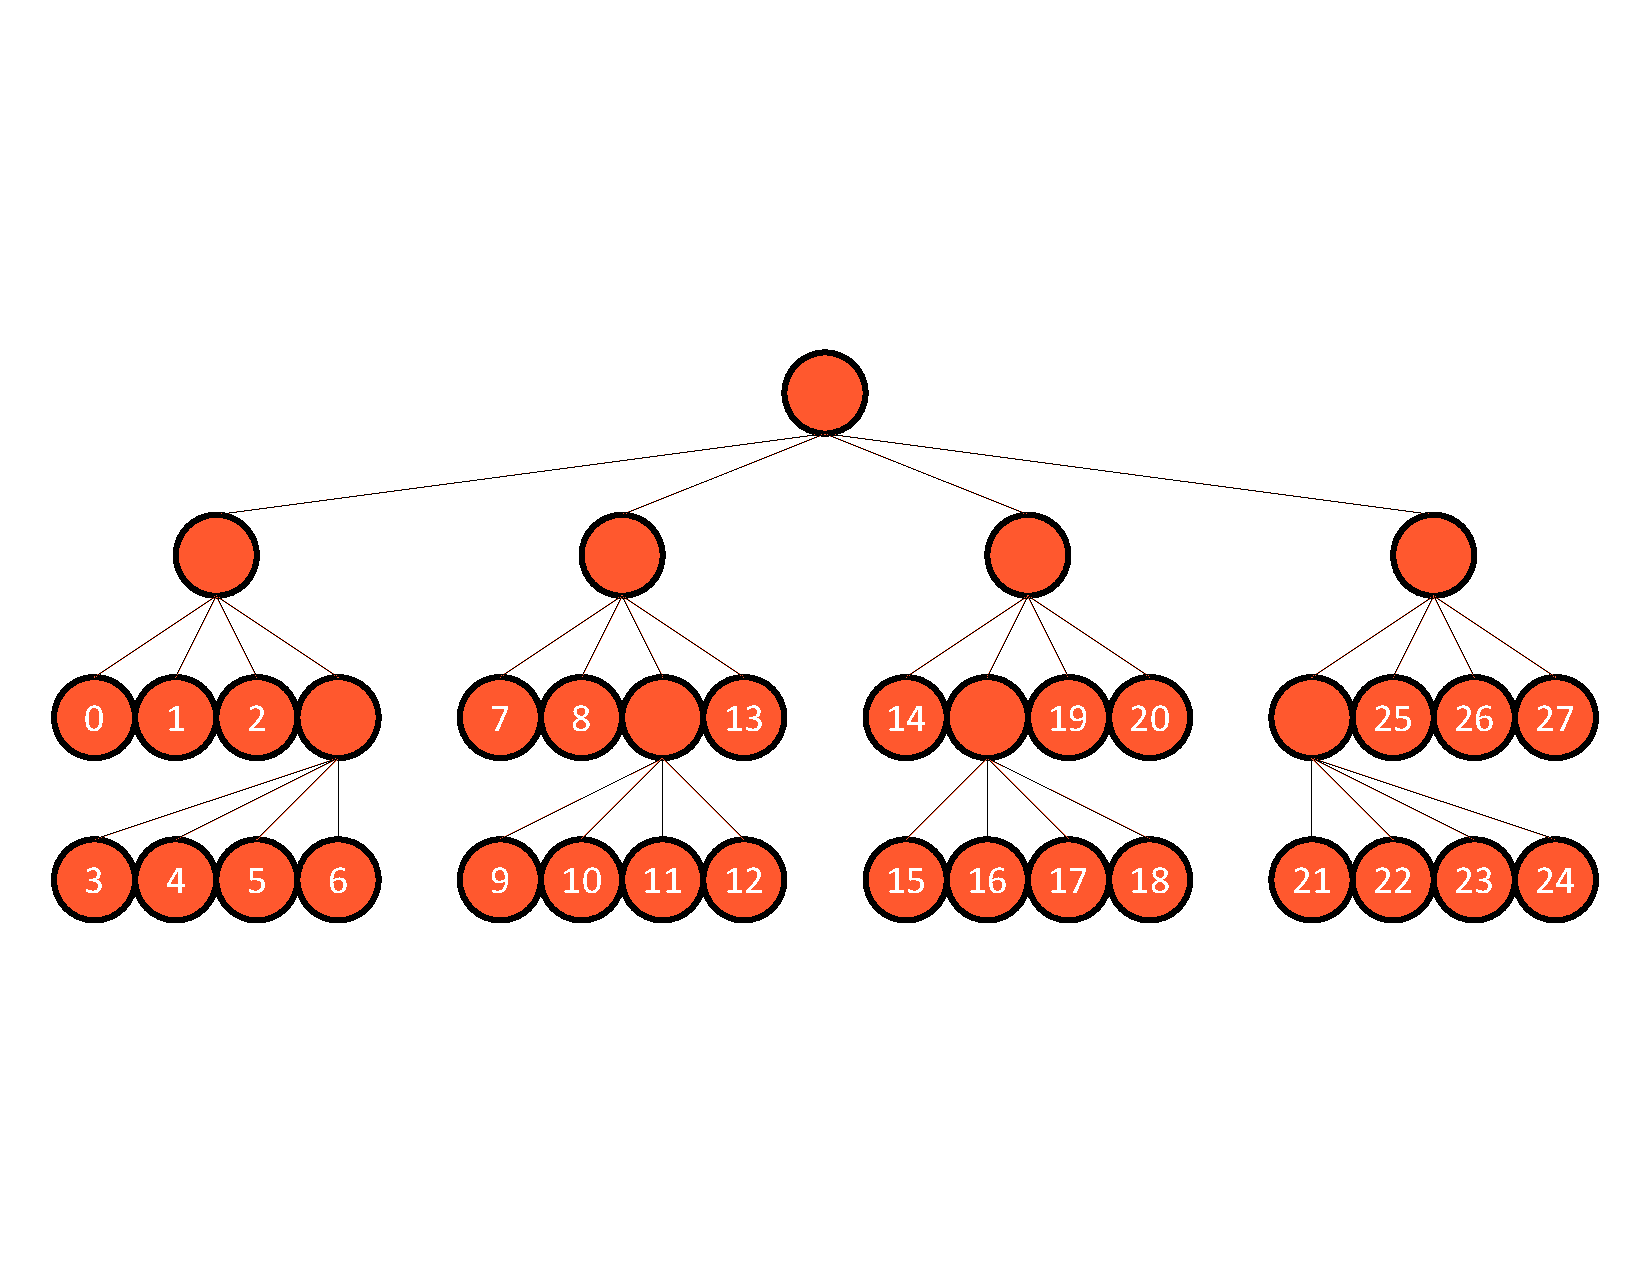
\includegraphics[width=\textwidth, clip=true, trim={0 150 0 150}]{../figures/leaf_indexing_tree.pdf}
        \caption{Leaf-level indexing of quadtree nodes}
    \end{subfigure}
    \\
    \begin{subfigure}[t]{0.8\textwidth}
        \centering
        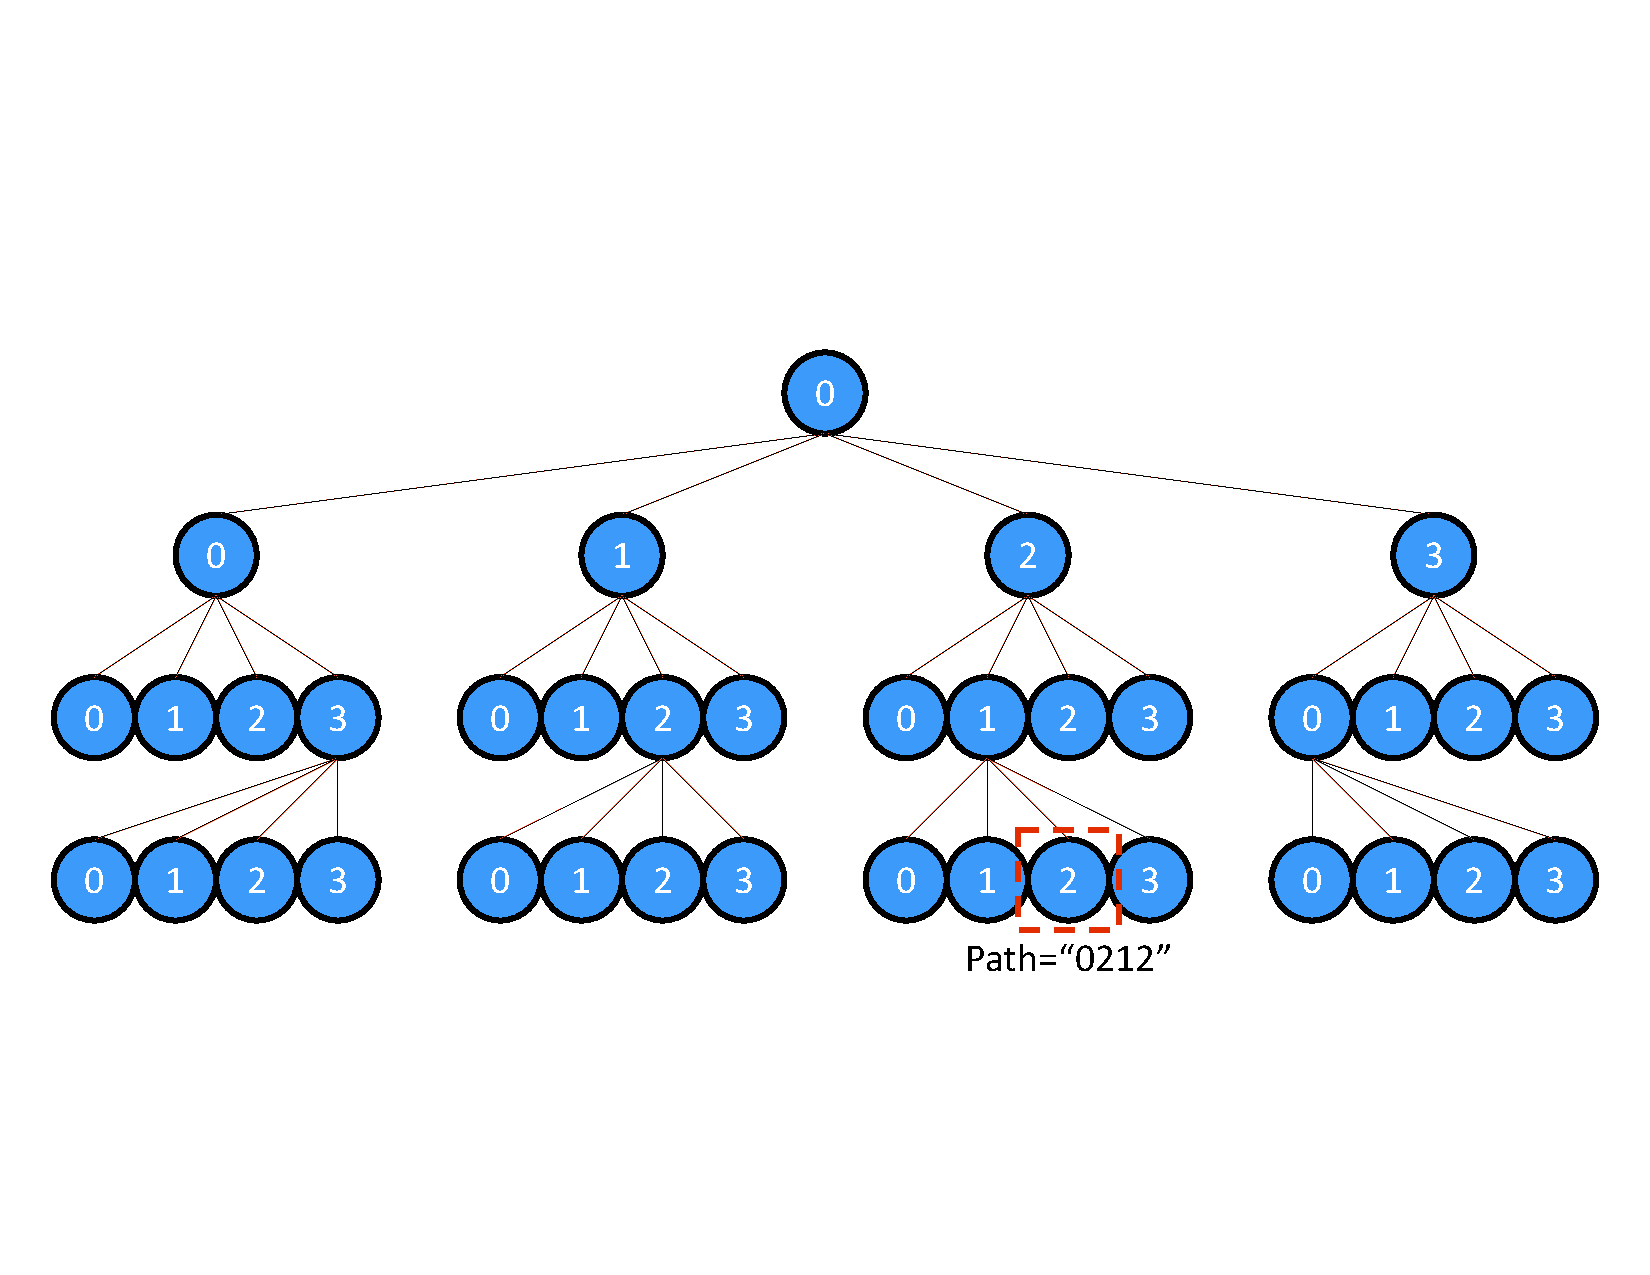
\includegraphics[width=\textwidth, clip=true, trim={0 140 0 150}]{../figures/global_indexing_tree.pdf}
        \caption{Path indexing of quadtree nodes}
    \end{subfigure}
\end{tabular}\\
\caption{Leaf-indexed vs. path-indexed quadtrees. In (a), only the leaves of a quadtree are indexed and stored. In (b), all nodes of the quadtree are indexed and stored according to their unique path.}
\label{fig:quadtree_indexing}
\end{figure}

\begin{figure}
\centering
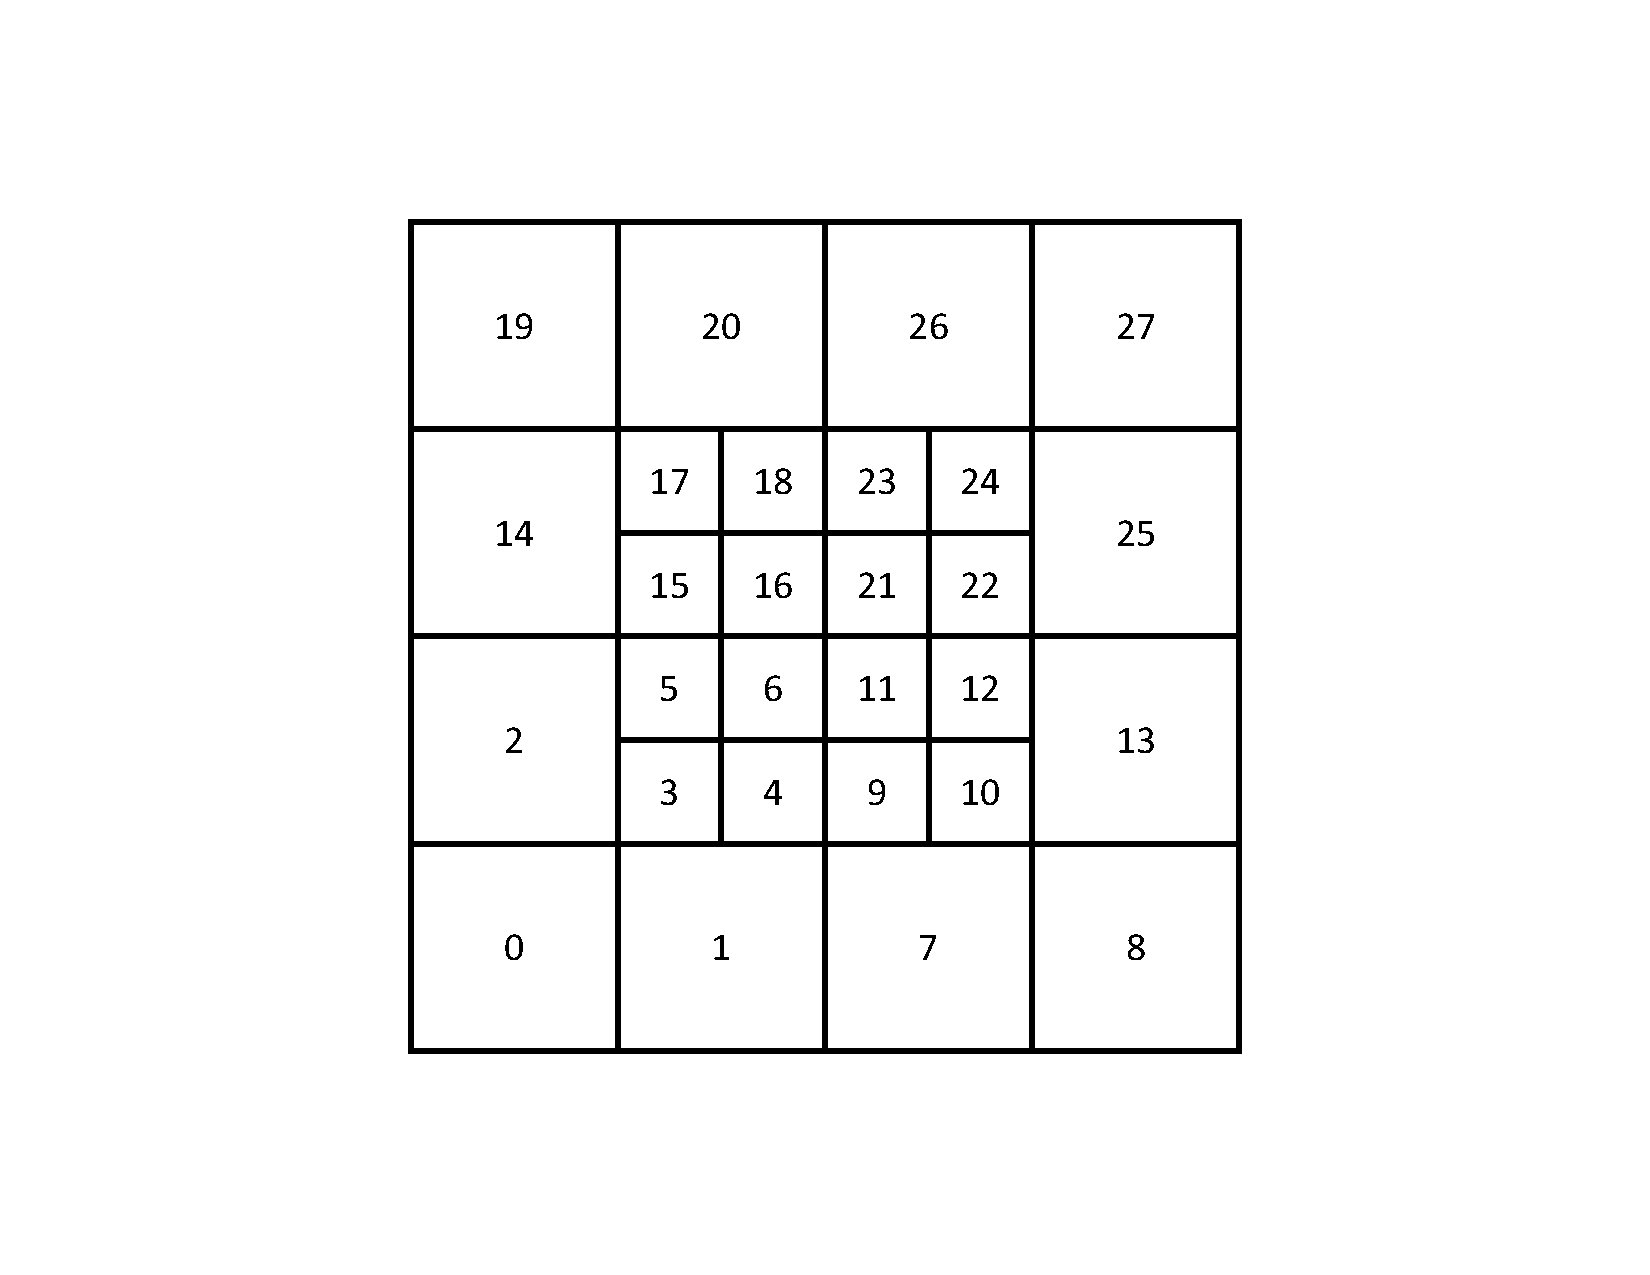
\includegraphics[width=0.4\textwidth]{../figures/adaptive_mesh_indexing.pdf}
\caption{A logically square domain is recursively broken into 4 children domains. This mesh represents refinement criteria that refines the center of the domain. The leaf level nodes are indexed according to a leaf-indexed quadtree and follow a space filling curve.}
\label{fig:adaptive_mesh}
\end{figure}

\ignore{As shown in \reffig{fig:quadtree_indexing}, each node in a family can be indexed $0$ to $3$. The highlighted node in \reffig{fig:quadtree_indexing} has a path of $0212$ which corresponds to the steps taken from the root to arrive at that node.}

\ignore{Quadtree data structures, including the path-indexed variety we use here, are not novel. One of the most notable uses of the quadtree data structure was for computer graphics (\cite{woodward1982explicit}, \cite{samet1984quadtree}). A quadtree data structure allows for hierarchical storage at different levels and is a natural application for recursive algorithms. Storing data at all nodes in a quadtree requires knowing the {\em path} of a node. The path of a node is the series of directions taken from the root of the tree to arrive at the particular node. Each node can be uniquely indexed according to the node's path. As shown in \reffig{fig:quadtree_indexing}, each node in a family can be indexed $0$ to $3$. The highlighted node in \reffig{fig:quadtree_indexing} has a path of $0212$ which corresponds to the steps taken from the root to arrive at that node.}

A path-indexed quadtree creates storage for all nodes in the tree through the use of a \texttt{NodeMap}, equivalent to a C++ \texttt{std::map<std::string, Node<T>*>}, where the template parameter \texttt{T} corresponds to a user-provided class to be stored at each node. For the quadtree-adaptive HPS method detailed in this paper, this is a class that holds patch data (grid information, matrices, and vectors). The path is computed by calling \texttt{p4est\_quadrant\_ancestor\_id}. The path-indexed quadtree wraps functions provided by \pforest to construct and iterate over nodes in the path-indexed quadtree.

Two functions provided by {\pforest} allow for a depth-first traversal of a {\pforest} quadtree: \texttt{p4est\_search\_all} and \texttt{p4est\_search\_reorder}. \texttt{p4est\_search\_all} performs a top-down search of the quadtree and provides a callback function with access to a {\pforest} quadrant data structure. This function is used to initialize the path-indexed quadtree by traversing the quadtree in a depth-first order, computing the path for each node, and allocating memory for a \texttt{Node} object in the \texttt{NodeMap}. The function \texttt{p4est\_search\_reorder} also does a top-down search, and provides pre- and post-quadrant callback functions for accessing quadrant data.

Wrapping \texttt{p4est\_search\_reorder}, we define the {\em merge traversal} and the {\em split traversal} of a quadtree. The merge traversal iterates over a quadtree in a post-order fashion, visiting children then parents. When visiting a leaf, a leaf callback is called. When visiting parents, a family callback is used that provides access to the parent and the four children nodes. This is to ``merge'' four children nodes into a parent node, after any leaf data is assigned or computed. The split traversal iterates over a quadtree in a pre-order fashion, with callbacks to families then leaf nodes. This is to provide access to families to ``split'' one parent node into four children nodes. The leaf callback is done last in the split traversal and is used to compute leaf level data once the entire tree has been traversed. The algorithm for the callback function passed to \texttt{p4est\_search\_reorder} is provided in \refalg{alg:quadtree_callback}.

\begin{algorithm}
\caption{\texttt{QuadtreeCallback} Function}
\begin{algorithmic}[0]
    \Require Functions \texttt{LeafCallback}(\texttt{leaf\_node}) \& \texttt{FamilyCallback}(\texttt{parent\_node, children\_nodes})
    \State Compute \texttt{path} from \texttt{p4est\_quadrant\_ancestor\_id}
    \State Let \texttt{node = node\_map[path]}
    \If{\texttt{node} is a leaf} \Comment{Node is a leaf, call leaf callback}
        \State Call \texttt{LeafCallback(node)}
    \Else \Comment{Node is a branch, get children and call family callback}
        \For{i = 0, 1, 2, 3}
            \State \texttt{children\_nodes[i] = map[path + string(i)]}
        \EndFor
        \State Call \texttt{FamilyCallback(node, children\_nodes)}
    \EndIf
\end{algorithmic}
\label{alg:quadtree_callback}
\end{algorithm}

For the quadtree-adaptive HPS method, the leaf callback for the merge traversal is \texttt{BuildD2N}, which solves \refeq{eq:map_D2N} and computes a leaf level Dirichlet-to-Neumann matrix. The family callback wraps the algorithms found in \refsec{sub:4-to-1merge}, which performs the 4-to-1 merge.

The family callback for the split traversal wraps \refeq{eq:solve_eqn}, which applies the solution operator to map parent Dirichlet data to children Dirichlet data (the 1-to-4 split). The leaf callback wraps \texttt{PatchSolver} to solve \refeq{eq:elliptic_pde} on a leaf level using fast solution methods.
\section{Numerical Results}
\label{sec:results}

To test and verify the implementation of the quadtree-adaptive HPS method, we solve two Poisson equations and one Helmholtz equation. For each, we present error, timing, and memory usage results and discuss the performance of our implemented method.

For all of our examples, we discretize the Laplace operator at the patch level using a second-order, 5-point stencil on a finite volume (cell-centered) mesh. The code, along with numerical experiments below, is stored in the GitHub repository EllipticForest \citep{chipman2023elliptic}. EllipticForest is written primarily in C++, with wrappers to FORTRAN routines to call FISHPACK and LAPACK (\citep{anderson1999lapack}) for any dense linear algebra operations. The mesh and solution are output into an unstructured VTK mesh file \citep{vtkBook} and are visualized with the VisIt software \citep{HPV:VisIt}. All tests were run on a 2021 MacBook Pro with an M1 Pro CPU and 32 GB of RAM.

\subsection{Poisson Equation 1}
\label{sub:example_one}

We solve the following boundary value problem:
\begin{align}
    \nabla^2 u(x,y) = -(\sin(x) + \sin(y))
\end{align}
on the square domain $\Omega = [-10, 10] \times [-10, 10]$, subject to Dirichlet boundary conditions $u(x,y) = g(x,y)$ on the boundary which is computed according to the exact solution
\begin{align}
    u_{exact}(x,y) &= \sin(x) + \sin(y).
\end{align}

For the refinement criteria, we refine according to the right-hand side function $f(x,y)$, which corresponds to the curvature of the solution. We set a refinement threshold of $1.2$ and refine a patch when $f(x,y) > 1.2$ for any $x,y$ in a patch. This results in a mesh and solution that can be found in \reffig{fig:poisson_plot}.

\begin{figure}
    \centering
    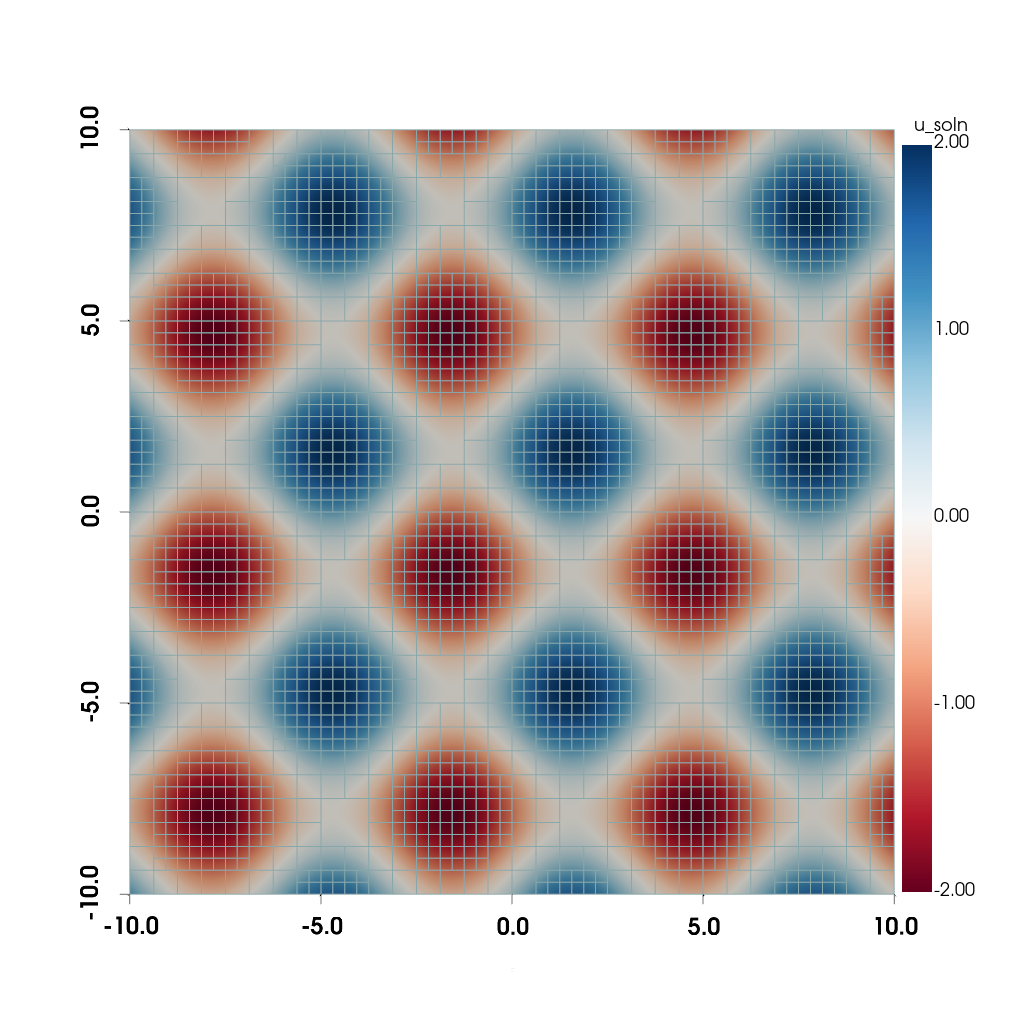
\includegraphics[width=0.75\textwidth, trim={0 100 0 0}]{figures/plot_poisson.png}
    \caption{The computed solution and mesh for the Poisson problem \refsec{sub:example_one}.  Patch size for this plot is $16 \times 16$ and mesh is refined to level 7.  Refinement criteria is based on the magnitude of the right hand side function $f(x,y)$.}
    \label{fig:poisson_plot}
\end{figure}

{\bf Results and Discussion}
Tables \ref{tab:poisson_error} and \ref{tab:poisson_timing} show the error, timing, and memory results for the current implementation on this Poisson equation. \reftab{tab:poisson_error} shows results for both a uniformly refined mesh (a mesh without any coarse-fine interfaces or local adaptivity) and results for the adaptive mesh case. For the uniform case, we get the expected second order convergence in both the $L_{\infty}$ and $L_1$ norms. The adaptive case mostly shows second order convergence, except for a few cases where the refinement between successive levels results in a smaller jump in error than second order provides. \reftab{tab:poisson_timing} shows timing and memory results for the same case. Here, the difference between the uniform and adaptive case is highlighted. The adaptive case gives a $4.5$ times speed up for the build stage, and nearly a $20$ times speed up for the solve stage. Memory used to store the quadtree and operators is also significantly reduced with the adaptive case.

% \begin{table}
%     \caption{TODO}
%     \begin{center}
%         \sisetup{
%             detect-weight=true,
%             detect-inline-weight=math,
%             table-alignment-mode=format
%         }
%         \begin{tabular}{
%             S   % Max levels
%             S   % Effective resolution
%             S   % DOFs
%             S[scientific-notation=true, round-mode=places, round-precision=2]   % L-inf error
%             S[round-mode=places, round-precision=2]   % L-inf order
%             S[scientific-notation=true, round-mode=places, round-precision=2]   % L-1 error
%             S[round-mode=places, round-precision=2]   % L-1 order
%             S[round-mode=places, round-precision=3]   % Build time
%             S[round-mode=places, round-precision=3]   % Solve time
%             S[round-mode=places, round-precision=1]   % Memory size
%         }
% \hline
% {$L$} & {$R_{eff}$} & {DOFs} & {$L_{\infty}$ Error} & {$L_{\infty}$ Order} & {$L_1$ Error} & {$L_1$ Order} & {$T_{B}$ (sec)} & {$T_{S}$ (sec)} & {$B$ (MB)} \\
% \hline
% \num{1} & \num{32} & \num{1024} & \num{0.0727000000000000} & {--} & \num{0.0233000000000000} & {--} & \num{0.0017400000000000} & \num{0.0027700000000000} & \num{0.4280000000000000} \\
% \num{2} & \num{64} & \num{4096} & \num{0.0178000000000000} & \num{2.0300781229532000} & \num{0.0057600000000000} & \num{2.0161892380993300} & \num{0.0120000000000000} & \num{0.0146000000000000} & \num{2.8400000000000000} \\
% \num{3} & \num{128} & \num{16384} & \num{0.0044600000000000} & \num{1.9967616259334600} & \num{0.0014400000000000} & \num{2.0000000000000000} & \num{0.0684000000000000} & \num{0.0448000000000000} & \num{15.9000000000000000} \\
% \num{4} & \num{256} & \num{65536} & \num{0.0011100000000000} & \num{2.0064840335702000} & \num{0.0003590000000000} & \num{2.0040130625066200} & \num{1.4400000000000000} & \num{0.1910000000000000} & \num{81.5000000000000000} \\
% \num{5} & \num{512} & \num{262144} & \num{0.0002790000000000} & \num{1.9922226494082800} & \num{0.0000897000000000} & \num{2.0008039537911500} & \num{7.2000000000000000} & \num{0.8940000000000000} & \num{398.0000000000000000} \\
% \num{6} & \num{1024} & \num{1048576} & \num{0.0000696000000000} & \num{2.0031059108678200} & \num{0.0000224000000000} & \num{2.0016092528616600} & \num{34.1000000000000000} & \num{3.8600000000000000} & \num{1880.0000000000000000} \\
% \num{7} & \num{2048} & \num{4194304} & \num{0.0000174000000000} & \num{2.0000000000000000} & \num{0.0000056100000000} & \num{1.9974260563361700} & \num{160.0000000000000000} & \num{19.0000000000000000} & \num{8680.0000000000000000} \\
% \hline
%         \end{tabular}
%     \end{center}
% \end{table}

\begin{table}
    \caption{Convergence analysis for Poisson's equation. The upper part shows convergence for a uniformly refined mesh, while the lower part shows convergence for an adaptively refined mesh. $M$ is the size of the grid on each leaf patch, $L_{\text{max}}$ is the maximum level of refinement, $R_{\text{eff}}$ is the effective resolution for a uniformly refined mesh, DOFs is the total degrees of freedom (i.e., total mesh points), $L_{\infty}$ error is the infinity norm error, $L_{\infty}$ order is the infinity norm convergence order, $L_1$ error is the $1^{\text{st}}$ norm error, and $L_1$ order is the $1^{\text{st}}$ norm convergence order.}
    \centering
    \sisetup{
        table-alignment-mode=format
    }
    \begin{tabular}{
        |
        S   % Patch size
        S[table-column-width=0.8cm]   % Max level
        S[table-text-alignment=right, table-column-width=0.7cm]   % Effective resolution
        S[table-text-alignment=right, table-column-width=1.4cm]   % DOFs
        S[scientific-notation=true, round-mode=places, round-precision=2, table-column-width=1.65cm]   % L-inf error
        S[scientific-notation=false, exponent-mode=fixed, round-mode=places, round-precision=2, table-column-width=1.5cm]   % L-inf order
        S[scientific-notation=true, round-mode=places, round-precision=2]   % L-1 error
        S[scientific-notation=false, exponent-mode=fixed, round-mode=places, round-precision=2]   % L-1 order
        |
    }
\hline
{M} & {$L_{\text{max}}$} & {$R_{\text{eff}}$} & {DOFs} & {$L_{\infty}$ Error} & {$L_{\infty}$ Order} & {$L_1$ Error} & {$L_1$ Order} \\
\hline
% \num{16} & \num{1} & \num{32} & \num{1024} & \num{7.2721827038740E-02} & {--} & \num{2.3319531214882E-02} & {--} \\
% \num{16} & \num{2} & \num{64} & \num{4096} & \num{1.7803276283615E-02} & \num{2.0302456853013E+00} & \num{5.7570511934287E-03} & \num{2.0181368404886E+00} \\
% \num{16} & \num{3} & \num{128} & \num{16384} & \num{4.4594278588197E-03} & \num{1.9972122300096E+00} & \num{1.4365857848192E-03} & \num{2.0026858961169E+00} \\
\num{16} & \num{4} & \num{256} & \num{65536} & \num{1.1146466297640E-03} & \num{2.0002722123237E+00} & \num{3.5892082197986E-04} & \num{2.0009066196875E+00} \\
\num{16} & \num{5} & \num{512} & \num{262144} & \num{2.7855514231123E-04} & \num{2.0005515585727E+00} & \num{8.9717104596707E-05} & \num{2.0002106534890E+00} \\
\num{16} & \num{6} & \num{1024} & \num{1048576} & \num{6.9642847198903E-05} & \num{1.9999158585307E+00} & \num{2.2428541266291E-05} & \num{2.0000472698832E+00} \\
\num{16} & \num{7} & \num{2048} & \num{4194304} & \num{1.7410906046011E-05} & \num{1.9999839043577E+00} & \num{5.6070914295010E-06} & \num{2.0000112920243E+00} \\
% \num{32} & \num{1} & \num{64} & \num{4096} & \num{1.7803276283615E-02} & {--} & \num{5.7570511934284E-03} & {--} \\
% \num{32} & \num{2} & \num{128} & \num{16384} & \num{4.4594278588175E-03} & \num{1.9972122300103E+00} & \num{1.4365857848190E-03} & \num{2.0026858961170E+00} \\
% \num{32} & \num{3} & \num{256} & \num{65536} & \num{1.1146466297716E-03} & \num{2.0002722123132E+00} & \num{3.5892082198209E-04} & \num{2.0009066196784E+00} \\
\num{32} & \num{4} & \num{512} & \num{262144} & \num{2.7855514234232E-04} & \num{2.0005515584215E+00} & \num{8.9717104608167E-05} & \num{2.0002106533137E+00} \\
\num{32} & \num{5} & \num{1024} & \num{1048576} & \num{6.9642847325024E-05} & \num{1.9999158560790E+00} & \num{2.2428541313515E-05} & \num{2.0000472670298E+00} \\
\num{32} & \num{6} & \num{2048} & \num{4194304} & \num{1.7410906499649E-05} & \num{1.9999838693813E+00} & \num{5.6070916187308E-06} & \num{2.0000112463735E+00} \\
\hline
% \num{16} & \num{1} & \num{32} & \num{1024} & \num{7.2721827038740E-02} & {--} & \num{2.3319531214882E-02} & {--} \\
% \num{16} & \num{2} & \num{64} & \num{4096} & \num{1.7803276283615E-02} & \num{2.0302456853013E+00} & \num{5.7570511934287E-03} & \num{2.0181368404886E+00} \\
% \num{16} & \num{3} & \num{128} & \num{16384} & \num{4.4594278588197E-03} & \num{1.9972122300096E+00} & \num{1.4365857848192E-03} & \num{2.0026858961169E+00} \\
\num{16} & \num{4} & \num{256} & \num{64000} & \num{2.5910957992683E-03} & \num{7.8329626881446E-01} & \num{4.4586170147130E-04} & \num{1.6879759592817E+00} \\
\num{16} & \num{5} & \num{512} & \num{194560} & \num{6.6263501289099E-04} & \num{1.9672760156010E+00} & \num{1.2477150864153E-04} & \num{1.8373077457909E+00} \\
\num{16} & \num{6} & \num{1024} & \num{569344} & \num{6.8094879278413E-04} & \num{-3.9331876110758E-02} & \num{1.0216613949030E-04} & \num{2.8837140596648E-01} \\
\num{16} & \num{7} & \num{2048} & \num{1984000} & \num{1.7141451745961E-04} & \num{1.9900570123994E+00} & \num{3.7577025980665E-05} & \num{1.4429943340785E+00} \\
% \num{32} & \num{1} & \num{64} & \num{4096} & \num{1.7803276283615E-02} & {--} & \num{5.7570511934284E-03} & {--} \\
% \num{32} & \num{2} & \num{128} & \num{16384} & \num{4.4594278588175E-03} & \num{1.9972122300103E+00} & \num{1.4365857848190E-03} & \num{2.0026858961170E+00} \\
% \num{32} & \num{3} & \num{256} & \num{65536} & \num{1.1146466297716E-03} & \num{2.0002722123132E+00} & \num{3.5892082198209E-04} & \num{2.0009066196784E+00} \\
\num{32} & \num{4} & \num{512} & \num{256000} & \num{6.6189922864102E-04} & \num{7.5190291839197E-01} & \num{1.1198962819648E-04} & \num{1.6803004955197E+00} \\
\num{32} & \num{5} & \num{1024} & \num{784384} & \num{1.6733508690897E-04} & \num{1.9838716073808E+00} & \num{3.1111362539336E-05} & \num{1.8478516397654E+00} \\
\num{32} & \num{6} & \num{2048} & \num{2289664} & \num{1.7139947044398E-04} & \num{-3.4622669955039E-02} & \num{2.5679498208238E-05} & \num{2.7682456821605E-01} \\
\hline
    \end{tabular}
    \label{tab:poisson_error}
\end{table}

\begin{table}
    \caption{Timing and memory results for Poisson's equation. The upper part shows results for the uniformly refined mesh, while the lower part shows results for the adaptively refined mesh. The results here are for a patch size of $16 \times 16$. $L_{\text{max}}$ is the maximum level of refinement, $R_{\text{eff}}$ is the effective resolution, DOFs is the total degrees of freedom, $T_{\text{build}}$ is the time in seconds for the build stage, $T_{\text{upwards}}$ is the time in seconds for the upwards stage, $T_{\text{solve}}$ is the time in seconds for the solve stage, and $S$ is the memory storage in megabytes to store the quadtree and all data matrices stored in each node of the quadtree.}
    \centering
    \sisetup{
        table-alignment-mode=format
    }
    \begin{tabular}{
        |
        S   % Max level
        S[table-text-alignment=right]   % Effective resolution
        S[table-text-alignment=right]   % Total DOFs
        S[table-text-alignment=right, scientific-notation=false, round-mode=places, round-precision=3]   % Build time
        S[table-text-alignment=right, scientific-notation=false, exponent-mode=fixed, round-mode=places, round-precision=3]   % Upwards time
        S[table-text-alignment=right, scientific-notation=false, round-mode=places, round-precision=3]   % Solve time
        S[table-text-alignment=right, scientific-notation=false, round-mode=places, round-precision=1]   % Memory size
        |
    }
\hline
{$L_{\text{max}}$} & {$R_{\text{eff}}$} & {DOFs} & {$T_{\text{build}}$ (sec)} & {$T_{\text{upwards}}$ (sec)} & {$T_{\text{solve}}$ (sec)} & {$S$ (MB)} \\
\hline
% \num{1} & \num{32} & \num{1024} & \num{0.015641083000000} & \num{1.07767500000000E-02} & \num{0.020481166000000} & \num{0.428303718566894} \\
% \num{2} & \num{64} & \num{4096} & \num{0.085338584000000} & \num{2.00472499999999E-02} & \num{0.036223209000000} & \num{2.843113899230950} \\
% \num{3} & \num{128} & \num{16384} & \num{0.393952542000000} & \num{7.48480829999999E-02} & \num{0.059746333000000} & \num{15.882237434387200} \\
\num{4} & \num{256} & \num{65536} & \num{2.031286957999990} & \num{3.66539416999999E-01} & \num{0.211029084000000} & \num{81.548497200012200} \\
\num{5} & \num{512} & \num{262144} & \num{8.525974832999990} & \num{1.77923349999999E+00} & \num{1.073760000000000} & \num{398.233067512512000} \\
\num{6} & \num{1024} & \num{1048576} & \num{39.353658666999900} & \num{9.00205208400000E+00} & \num{4.258692584000000} & \num{1881.010411262510000} \\
\num{7} & \num{2048} & \num{4194304} & \num{172.189544875000000} & \num{4.20349420419999E+01} & \num{20.559359582999900} & \num{8676.197911262510000} \\
\hline
% \num{1} & \num{32} & \num{1024} & \num{0.010200834000000} & \num{2.31674999999999E-03} & \num{0.013967208000000} & \num{0.428303718566894} \\
% \num{2} & \num{64} & \num{4096} & \num{0.077488417000000} & \num{1.34400419999999E-02} & \num{0.016857250000000} & \num{2.843113899230950} \\
% \num{3} & \num{128} & \num{16384} & \num{0.320450292000000} & \num{8.29752079999999E-02} & \num{0.049673459000000} & \num{15.882237434387200} \\
\num{4} & \num{256} & \num{64000} & \num{1.502292208999990} & \num{3.93616458000000E-01} & \num{0.098160250000000} & \num{52.977078437805100} \\
\num{5} & \num{512} & \num{194560} & \num{3.718632625000000} & \num{9.24946582999999E-01} & \num{0.290812499999999} & \num{140.070134162902000} \\
\num{6} & \num{1024} & \num{569344} & \num{10.594630750000000} & \num{2.22070095800000E+00} & \num{0.478022832999999} & \num{368.462132453918000} \\
\num{7} & \num{2048} & \num{1984000} & \num{38.976778125000000} & \num{8.09454862499999E+00} & \num{1.838669208000000} & \num{1443.861859321590000} \\
\hline
    \end{tabular}
    \label{tab:poisson_timing}
\end{table}

\subsection{Poisson Equation 2 (Polar-Star Problem)}

As another test for Poisson's equation, we solve a ``polar star'' Poisson problem. The problem is created via a method of manufactured solutions and is engineered to have highly local curvature from the load function. The resulting solution is a collection of polar stars with user specified number of points and radii of curvature. This problem highlights the use of an adaptive mesh to solve the elliptic equation. The exact solution we attempt to reconstruct is the following:
\begin{align}
    u(x,y) = \frac{1}{2} \sum_{i=1}^{N} 1 - \tanh \left(\frac{r(x,y)-r_{0,i} \left(r_{1,i} \cos \left(n \theta(x,y)\right)+1\right)}{\epsilon }\right)
\end{align}
Computing the Laplacian analytically yields the right-hand side to Poisson's equation. Thus, the polar star Poisson problem is defined as follows:
\begin{align}
    \nabla^2 u(x,y) = \sum_{i=1}^N -\frac{s_{1,i}(x,y) + s_{2,i}(x, y)}{r(x,y)^2} - s_{3,i}(x,y) + s_{4,i}(x,y)
\end{align}
with
\begin{align*}
    s_{1,i}(x,y) &= \frac{p(x,y)^2 \tanh \left(\phi(x,y)\right) \text{sech}^2\left(\phi(x,y)\right)}{\epsilon ^2} \\
    s_{2,i}(x,y) &= -\frac{n^2 r_{0,i} r_{1,i} \cos (n \theta(x,y)) \text{sech}^2\left(\phi(x,y)\right)}{2 \epsilon } \\
    s_{3,i}(x,y) &= \frac{\tanh \left(\phi(x,y)\right) \text{sech}^2\left(\phi(x,y)\right)}{\epsilon ^2} \\
    s_{4,i}(x,y) &= \frac{\text{sech}^2\left(\phi(x,y)\right)}{2 r(x,y) \epsilon } \\
    p(x,y) &= n r_{0,i} r_{1,i} \sin (n \theta(x,y)) \\
    \phi(x,y) &= \frac{r(x,y)-r_{0,i} (r_{1,i} \cos (n \theta(x,y))+1)}{\epsilon}
\end{align*}
and where $i=1, ..., N_{polar}$ and $N_{polar}$ is the number of polar stars. Each polar star has a center $(x_0, y_0)$, inner and outer radii $r_0, r_1$, and the number of arms per polar star $n$. The radius and angle have the standard polar transforms:
\begin{align}
    r(x,y) &= \sqrt{(x - x_0)^2 + (y - y_0)^2} \\
    \theta(x,y) &= \tan^{-1}\Big(\frac{y - y_0}{x - x_0}\Big)
\end{align}
\reftab{table:polar_star_parameters} has the parameters used in this case study. \reffig{fig:polar_star_plot} shows the resulting mesh and solution. \reftab{tab:polar_star_results} shows the error, timing, and memory results for the polar star Poisson problem.
\begin{table}[ht]
    \begin{center}
        \caption{Polar Star Poisson Problem Parameters}
        \begin{tabular}{|c|c|c|c|c|c|}
            \hline
            $i$ & $x_0$ & $y_0$ & $r_0$ & $r_1$ & $n$ \\
            \hline
            $1$ & $-0.5$ & $-0.5$ & $0.2$ & $0.3$ & $3$ \\
            $2$ & $0.5$ & $-0.5$ & $0.3$ & $0.4$ & $4$ \\
            $3$ & $0$ & $0.5$ & $0.4$ & $0.5$ & $5$ \\
            \hline
        \end{tabular}
        \label{table:polar_star_parameters}
    \end{center}
\end{table}

\begin{figure}
    \centering
    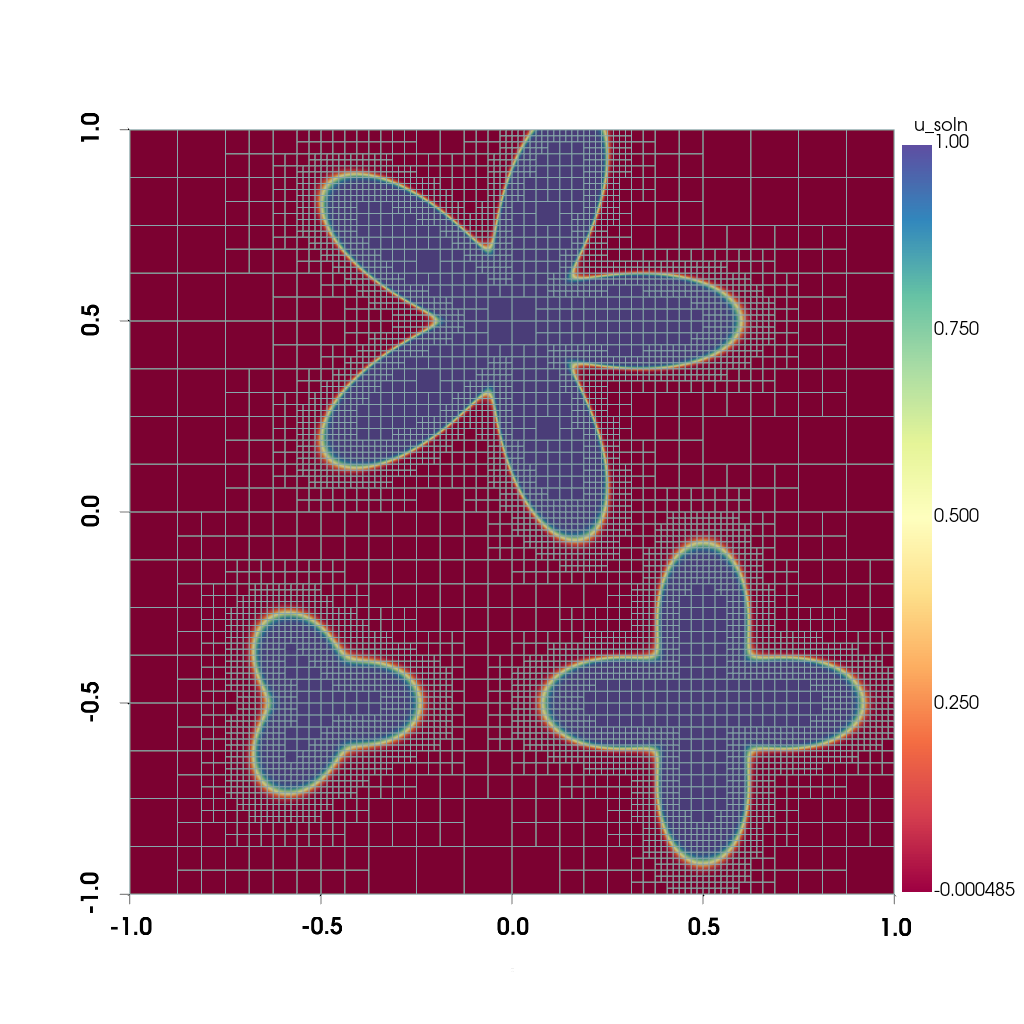
\includegraphics[width=0.75\textwidth, trim={0 100 0 0}]{figures/plot_polar_star.png}
    \caption{The computed solution and mesh for the Polar Star Poisson problem. Each patch has a $16 \times 16$ cell-centered grid. The mesh is refined according to the right-hand side and is refined with 8 levels of refinement.}
    \label{fig:polar_star_plot}
\end{figure}

\begin{table}
    \caption{Convergence analysis for the Polar Star Poisson problem. The upper part shows convergence for a uniformly refined mesh, while the lower part shows convergence for an adaptively refined mesh. $M$ is the size of the grid on each leaf patch, $L_{\text{max}}$ is the maximum level of refinement, $R_{\text{eff}}$ is the effective resolution for a uniformly refined mesh, DOFs is the total degrees of freedom (i.e., total mesh points), $L_{\infty}$ error is the infinity norm error, $L_{\infty}$ order is the infinity norm convergence order, $L_1$ error is the $1^{\text{st}}$ norm error, and $L_1$ order is the $1^{\text{st}}$ norm convergence order.}
    \centering
    \sisetup{
        table-alignment-mode=format
    }
    \begin{tabular}{
        |
        S   % Patch size
        S[table-column-width=0.8cm]   % Max level
        S[table-text-alignment=right, table-column-width=0.7cm]   % Effective resolution
        S[table-text-alignment=right, table-column-width=1.4cm]   % DOFs
        S[scientific-notation=true, round-mode=places, round-precision=2, table-column-width=1.65cm]   % L-inf error
        S[scientific-notation=false, exponent-mode=fixed, round-mode=places, round-precision=2, table-column-width=1.5cm]   % L-inf order
        S[scientific-notation=true, round-mode=places, round-precision=2]   % L-1 error
        S[scientific-notation=false, exponent-mode=fixed, round-mode=places, round-precision=2]   % L-1 order
        |
    }
\hline
{M} & {$L_{\text{max}}$} & {$R_{\text{eff}}$} & {DOFs} & {$L_{\infty}$ Error} & {$L_{\infty}$ Order} & {$L_1$ Error} & {$L_1$ Order} \\
\hline
\num{16} & \num{4} & \num{256} & \num{65536} & \num{1.56199870806249E+00} & \num{3.03980331387296E+00} & \num{1.65069071070283E-01} & \num{4.25135175327624E+00} \\
\num{16} & \num{5} & \num{512} & \num{262144} & \num{2.79704505790678E-02} & \num{5.80334595545976E+00} & \num{9.84718059820731E-04} & \num{7.38914339546720E+00} \\
\num{16} & \num{6} & \num{1024} & \num{1048576} & \num{5.25422685067089E-03} & \num{2.41235309940473E+00} & \num{7.39997994016763E-05} & \num{3.73411745253242E+00} \\
\num{16} & \num{7} & \num{2048} & \num{4194304} & \num{1.28369442835374E-03} & \num{2.03317666696840E+00} & \num{1.84035492646184E-05} & \num{2.00753733205534E+00} \\
\num{32} & \num{3} & \num{256} & \num{65536} & \num{1.56199870806260E+00} & \num{3.03980331387287E+00} & \num{1.65069071070315E-01} & \num{4.25135175327601E+00} \\
\num{32} & \num{4} & \num{512} & \num{262144} & \num{2.79704505792760E-02} & \num{5.80334595544912E+00} & \num{9.84718059909330E-04} & \num{7.38914339533767E+00} \\
\num{32} & \num{5} & \num{1024} & \num{1048576} & \num{5.25422685134335E-03} & \num{2.41235309923083E+00} & \num{7.39997994074657E-05} & \num{3.73411745254936E+00} \\
\num{32} & \num{6} & \num{2048} & \num{4194304} & \num{1.28369443102049E-03} & \num{2.03317666415598E+00} & \num{1.84035493232030E-05} & \num{2.00753732757563E+00} \\
\hline
\num{16} & \num{4} & \num{256} & \num{50944} & \num{1.56155552227466E+00} & \num{3.04021270772076E+00} & \num{1.64990394749018E-01} & \num{4.25203954412867E+00} \\
\num{16} & \num{5} & \num{512} & \num{171520} & \num{7.12119724134531E-02} & \num{4.45472024347345E+00} & \num{1.03166637134095E-03} & \num{7.32126173153682E+00} \\
\num{16} & \num{6} & \num{1024} & \num{476416} & \num{9.14563250417531E-02} & \num{-3.60963136314842E-01} & \num{1.78815639727227E-04} & \num{2.52843166634489E+00} \\
\num{16} & \num{7} & \num{2048} & \num{1587712} & \num{2.81786611011458E-02} & \num{1.69847988484306E+00} & \num{6.32775510074655E-05} & \num{1.49870725401785E+00} \\
\num{32} & \num{3} & \num{256} & \num{65536} & \num{1.56199870806260E+00} & \num{3.03980331387287E+00} & \num{1.65069071070315E-01} & \num{4.25135175327601E+00} \\
\num{32} & \num{4} & \num{512} & \num{203776} & \num{2.79706867876203E-02} & \num{5.80333377204982E+00} & \num{9.84314973348746E-04} & \num{7.38973407206102E+00} \\
\num{32} & \num{5} & \num{1024} & \num{701440} & \num{2.33901397925928E-02} & \num{2.58015193873839E-01} & \num{8.15186205620300E-05} & \num{3.59391849705353E+00} \\
\num{32} & \num{6} & \num{2048} & \num{1921024} & \num{2.81786212280739E-02} & \num{-2.68700538645513E-01} & \num{3.10231851870699E-05} & \num{1.39378282159843E+00} \\
\hline
    \end{tabular}
    \label{tab:polar_star_results}
\end{table}

\begin{table}
    \caption{Timing and memory results for the Polar Star Poisson problem. The upper part shows results for the uniformly refined mesh, while the lower part shows results for the adaptively refined mesh. The results here are for a patch size of $16 \times 16$. $L_{\text{max}}$ is the maximum level of refinement, $R_{\text{eff}}$ is the effective resolution, DOFs is the total degrees of freedom, $T_{\text{build}}$ is the time in seconds for the build stage, $T_{\text{upwards}}$ is the time in seconds for the upwards stage, $T_{\text{solve}}$ is the time in seconds for the solve stage, and $S$ is the memory storage in megabytes to store the quadtree and all data matrices stored in each node of the quadtree.}
    \centering
    \sisetup{
        table-alignment-mode=format
    }
    \begin{tabular}{
        |
        S[table-column-width=0.8cm]   % Max level
        S[table-text-alignment=right, table-column-width=0.7cm]   % Effective resolution
        S[table-text-alignment=right, table-column-width=1.4cm]   % DOFs
        S[table-text-alignment=right, scientific-notation=false, exponent-mode=fixed, round-mode=places, round-precision=2]   % Build time
        S[table-text-alignment=right, scientific-notation=false, exponent-mode=fixed, round-mode=places, round-precision=2]   % Upwards time
        S[table-text-alignment=right, scientific-notation=false, exponent-mode=fixed, round-mode=places, round-precision=2]   % Solve time
        S[table-text-alignment=right, scientific-notation=false, exponent-mode=fixed, round-mode=places, round-precision=2]   % Memory size
        |
    }
\hline
{$L_{\text{max}}$} & {$R_{\text{eff}}$} & {DOFs} & {$T_{\text{build}}$ (sec)} & {$T_{\text{upwards}}$ (sec)} & {$T_{\text{solve}}$ (sec)} & {$S$ (MB)} \\
\hline
\num{4} & \num{256} & \num{65536} & \num{1.60620216600000E+00} & \num{4.159940420000E-01} & \num{2.08710665999999E-01} & \num{8.15484972000122E+01} \\
\num{5} & \num{512} & \num{262144} & \num{7.76756095899999E+00} & \num{1.969481791000E+00} & \num{9.65551166999999E-01} & \num{3.98233067512512E+02} \\
\num{6} & \num{1024} & \num{1048576} & \num{3.56706281669999E+01} & \num{9.239545625000E+00} & \num{4.09653733299999E+00} & \num{1.88101041126251E+03} \\
\num{7} & \num{2048} & \num{4194304} & \num{1.65943133041000E+02} & \num{4.246258775000E+01} & \num{1.93515662920000E+01} & \num{8.67619791126251E+03} \\
\hline
\num{4} & \num{256} & \num{50944} & \num{9.29590041999999E-01} & \num{2.385920420000E-01} & \num{8.11892919999999E-02} & \num{3.35243158340454E+01} \\
\num{5} & \num{512} & \num{171520} & \num{3.32502091600000E+00} & \num{7.851652910000E-01} & \num{1.44476500000000E-01} & \num{1.15864575386047E+02} \\
\num{6} & \num{1024} & \num{476416} & \num{9.06574687500000E+00} & \num{1.937123083000E+00} & \num{3.00085959000000E-01} & \num{2.95106141090393E+02} \\
\num{7} & \num{2048} & \num{1587712} & \num{3.07760261670000E+01} & \num{7.226564708000E+00} & \num{1.12108816699999E+00} & \num{1.07681472492218E+03} \\
\hline
    \end{tabular}
    \label{tab:polar_star_timing}
\end{table}

{\bf Results and Discussion}
The polar star Poisson problem is able to highlight the benefits of an adaptive mesh. As shown in \reffig{fig:polar_star_plot}, there is room for significant speed up on the areas outside each polar star. The localized curvature is sufficiently captured by this adaptive scheme. \reftab{tab:polar_star_results} show the error analysis for this problem. Because of the large curvature at the boundaries of a polar star and our use of a second-order accurate solver, the $L_{\infty}$ error is larger than the first Poisson equation from \refsec{sub:example_one}, but we can still achieve 6 digits of accuracy in the $L_1$ norm. The timing results shown in \reftab{tab:polar_star_timing} show significant speed up between the uniform and adaptive implementations. The build time has a $5.5$ times speed up, the upwards stage has a $5.8$ times speed up, and the solve stage has a $17$ times speed up. Plus, the memory for the adaptive case is about $1/8th$ of the memory required for the uniform case.

\subsection{Helmholtz's Equation}
\label{sub:helmholtz_equation}

We now seek to solve the boundary value problem
\begin{align}
    \nabla^2 u(x,y) + \lambda u(x,y) = f(x,y),
\end{align}
on the square domain $\Omega = [-0.5, 0.5] \times [-0.5, 0.5]$ and subject to Dirichlet boundary conditions which are supplied via the exact solution discussed below.

To provide an analytical solution to compare against, we use a problem provided in \citep{cheng2006adaptive} where they solve Helmholtz's equation on an adaptive mesh. The manufactured solution is
\begin{align}
    u(\textbf{x}) = \sum_{i=1}^{3} e^{-\alpha |\textbf{x} - \textbf{x}_i|^2}
\end{align}
with $\lambda=0.01$, $\alpha=50$, $\textbf{x}_1 = (0.1, 0.1)$, $\textbf{x}_2 = (0, 0)$, and $\textbf{x}_3 = (-0.15, 0.1)$. The right-hand side is computed analytical via the Mathematica software \citep{Mathematica} and is used as the refinement criteria. We set the threshold for refinement to $60$. The solution and right-hand side function for $16 \times 16$ patches are plotted in \reffig{fig:helmholtz_u_plot} and \reffig{fig:helmholtz_f_plot}.

{\bf Results and Discussion}
As demonstrated with this example, the implemented HPS solves Helmholtz equations as well with the expected second order accuracy. See \reftab{tab:helmholtz_results} for error and convergence analysis. The adaptive mesh is able to successfully capture the curvature and reduce the work required to solve this equation. \reftab{tab:helmholtz_timing} show timing and memory usage results, which show significant speedup due to good mesh adaptation. We achieve a $17$ times speedup for the build and upwards stage and a $57$ times speedup for the solve stage. Memory is also impressive for this particular problem, with solving the same problem with similar error with $4.6\%$ of the required memory.

% \begin{figure}
%     \centering
%     \begin{tabular}{c c}
%     \smallskip
%         \begin{subfigure}[t]{0.46\textwidth}
%             \centering
%             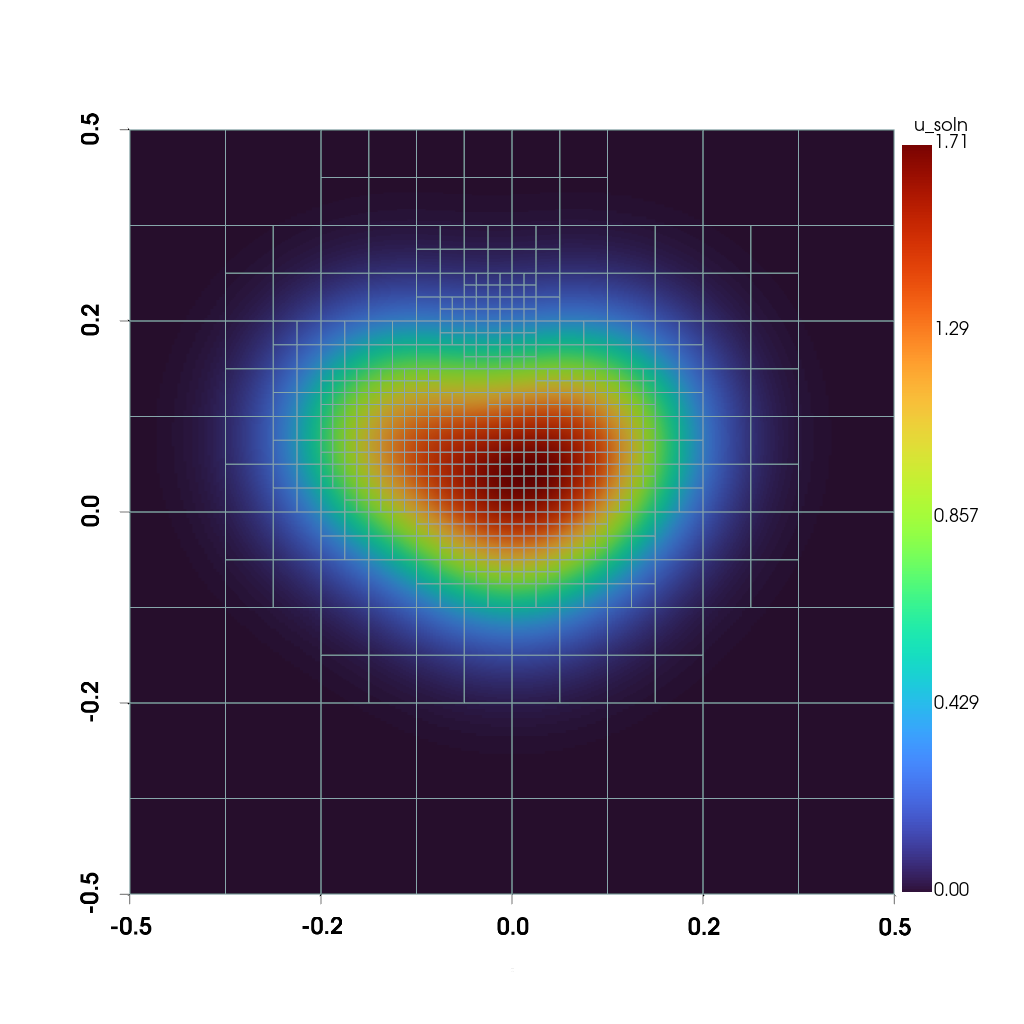
\includegraphics[width=\textwidth, clip=true, trim={0 80 0 0}]{figures/plot_helmholtz_u.png}
%         \end{subfigure}
%         &
%         \begin{subfigure}[t]{0.46\textwidth}
%             \centering
%             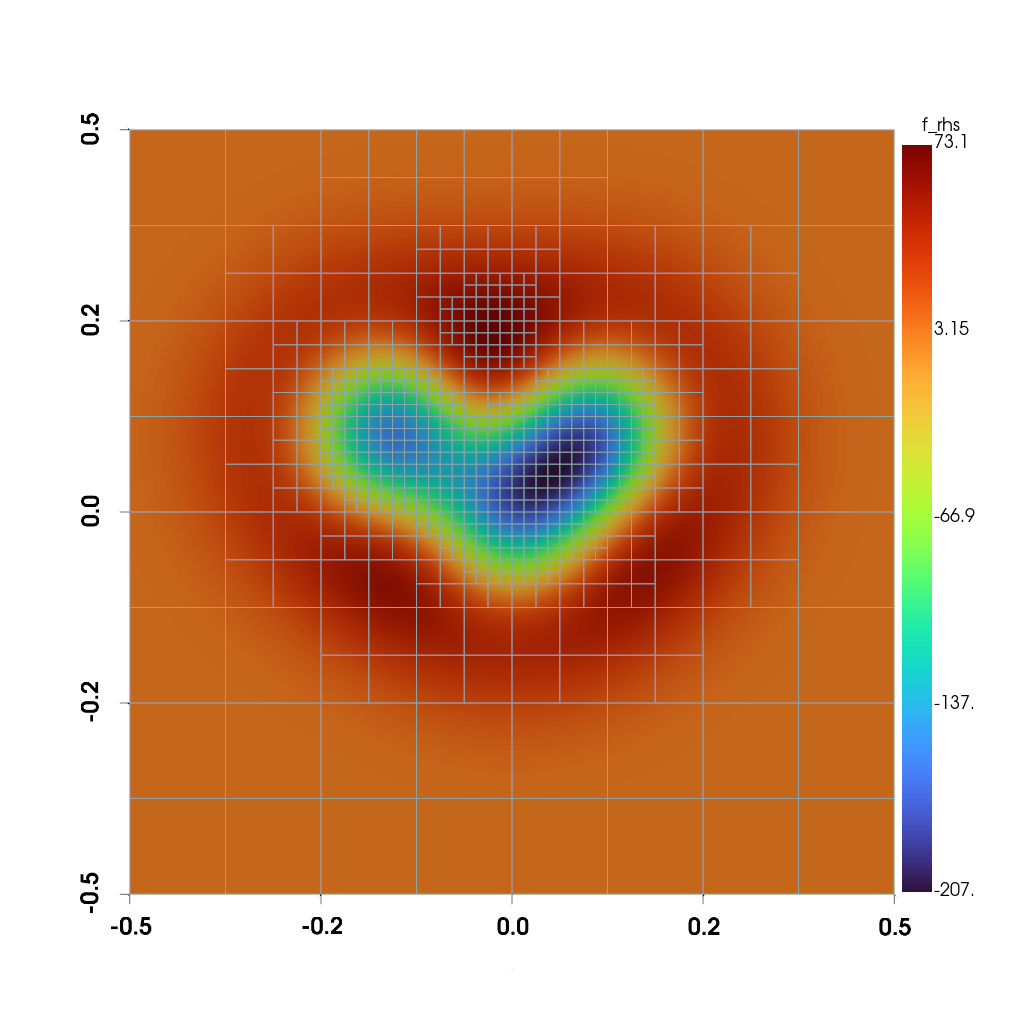
\includegraphics[width=\textwidth, clip=true, trim={0 80 0 0}]{figures/plot_helmholtz_f.png}
%         \end{subfigure}
%     \end{tabular}\\
%     \caption{Mesh and plot of Helmholtz's equations. The left plot is the computed solution and the right plot is the right-hand side.}
%     \label{fig:helmholtz_plots}
% \end{figure}

\begin{figure}
    \centering
    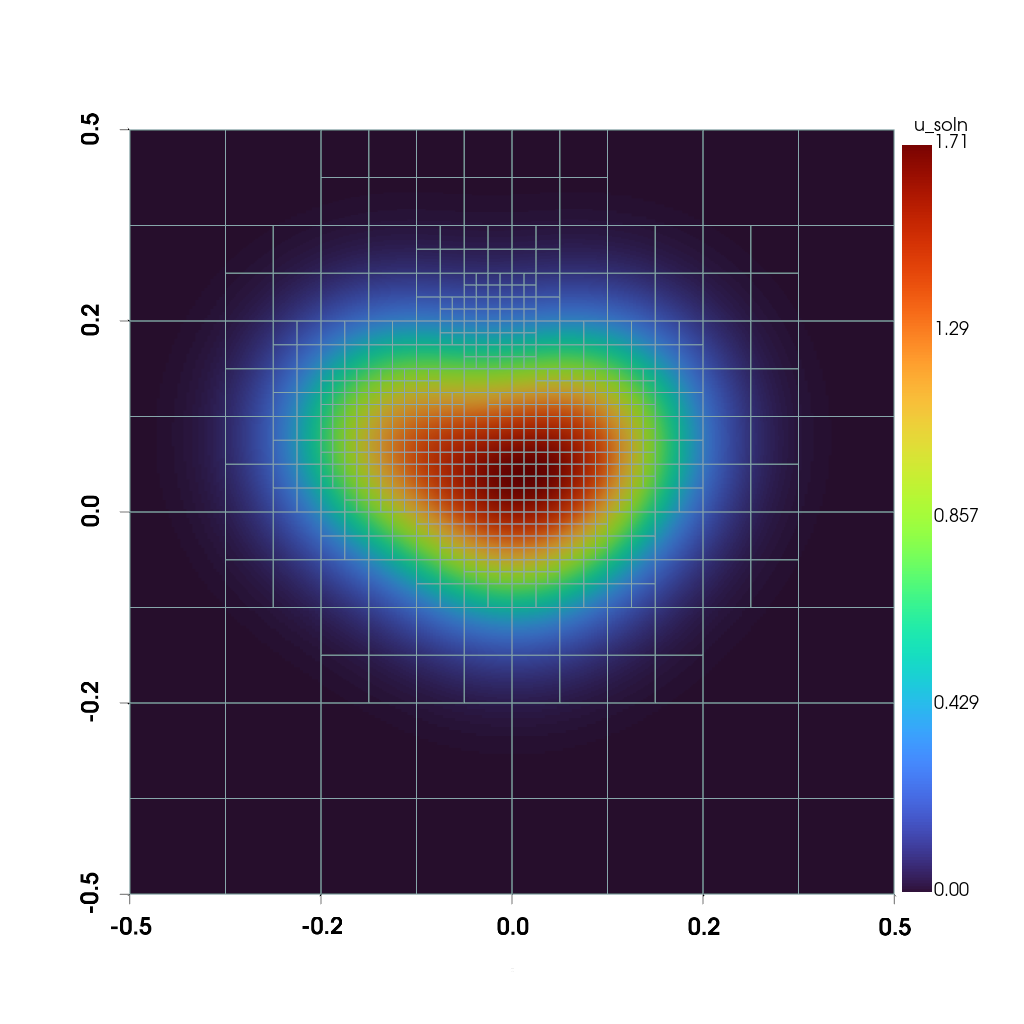
\includegraphics[width=0.75\textwidth, trim={0 100 0 0}]{figures/plot_helmholtz_u.png}
    \caption{Mesh and plot of the solution to the Helmholtz problem in \refsec{sub:helmholtz_equation}.}
    \label{fig:helmholtz_u_plot}
\end{figure}

\begin{figure}
    \centering
    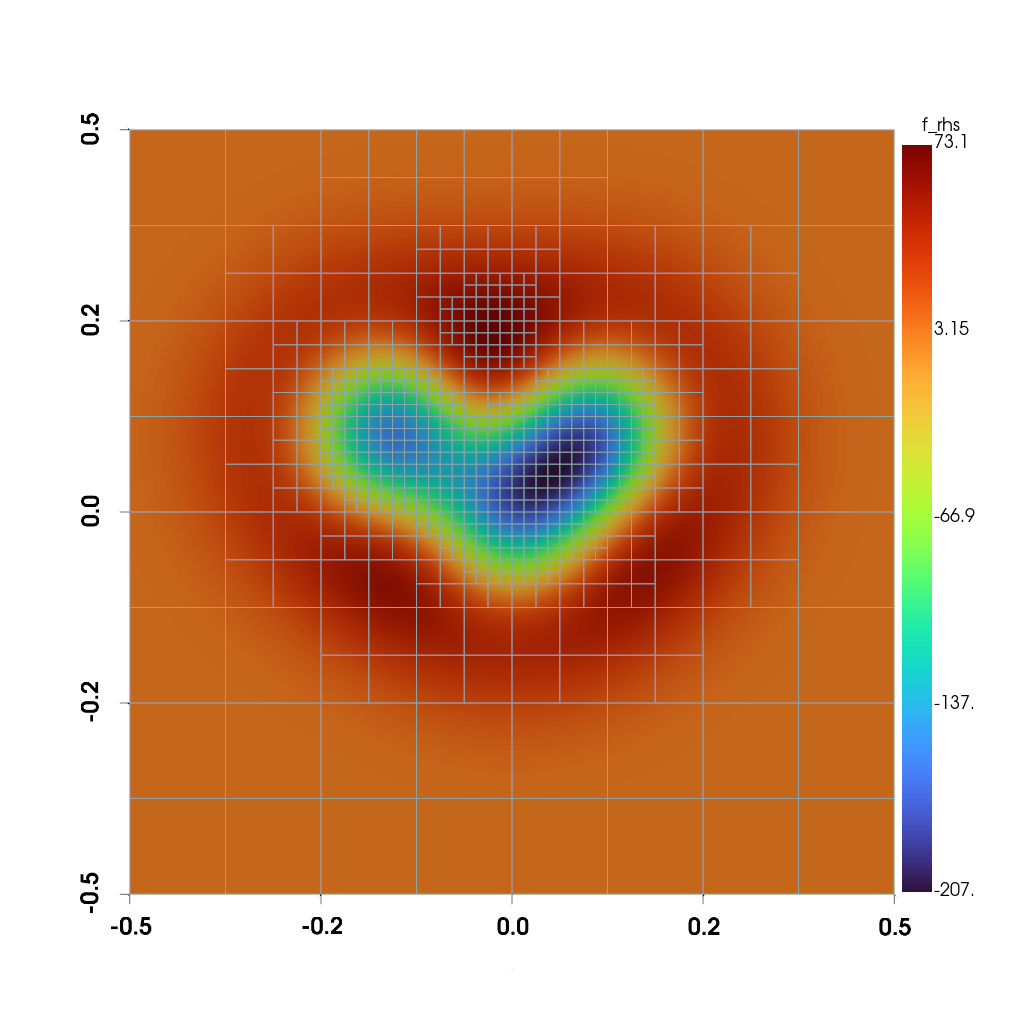
\includegraphics[width=0.75\textwidth, trim={0 100 0 0}]{figures/plot_helmholtz_f.png}
    \caption{Mesh and right-hand side of the solution to the Helmholtz problem in \refsec{sub:helmholtz_equation}.}
    \label{fig:helmholtz_f_plot}
\end{figure}

\begin{table}
    \caption{Convergence analysis for the Helmholtz problem. The upper part shows convergence for a uniformly refined mesh, while the lower part shows convergence for an adaptively refined mesh. $M$ is the size of the grid on each leaf patch, $L_{\text{max}}$ is the maximum level of refinement, $R_{\text{eff}}$ is the effective resolution for a uniformly refined mesh, DOFs is the total degrees of freedom (i.e., total mesh points), $L_{\infty}$ error is the infinity norm error, $L_{\infty}$ order is the infinity norm convergence order, $L_1$ error is the $1^{\text{st}}$ norm error, and $L_1$ order is the $1^{\text{st}}$ norm convergence order.}
    \centering
    \sisetup{
        table-alignment-mode=format
    }
    \begin{tabular}{
        |
        S   % Patch size
        S[table-column-width=0.8cm]   % Max level
        S[table-text-alignment=right, table-column-width=0.7cm]   % Effective resolution
        S[table-text-alignment=right, table-column-width=1.4cm]   % DOFs
        S[scientific-notation=true, round-mode=places, round-precision=2, table-column-width=1.65cm]   % L-inf error
        S[scientific-notation=false, exponent-mode=fixed, round-mode=places, round-precision=2, table-column-width=1.5cm]   % L-inf order
        S[scientific-notation=true, round-mode=places, round-precision=2]   % L-1 error
        S[scientific-notation=false, exponent-mode=fixed, round-mode=places, round-precision=2]   % L-1 order
        |
    }
\hline
{M} & {$L_{\text{max}}$} & {$R_{\text{eff}}$} & {DOFs} & {$L_{\infty}$ Error} & {$L_{\infty}$ Order} & {$L_1$ Error} & {$L_1$ Order} \\
\hline
% \num{16} & \num{1} & \num{32} & \num{1024} & \num{1.29237401760500E-02} & \num{0.00000000000000E+00} & \num{1.41621768661641E-03} & \num{0.00000000000000E+00} \\
% \num{16} & \num{2} & \num{64} & \num{4096} & \num{3.24474376001426E-03} & \num{1.99384719443466E+00} & \num{3.52042103641637E-04} & \num{2.00822315072563E+00} \\
\num{16} & \num{3} & \num{128} & \num{16384} & \num{8.11856103331010E-04} & \num{1.99880860589163E+00} & \num{8.79086298739653E-05} & \num{2.00167127817603E+00} \\
\num{16} & \num{4} & \num{256} & \num{65536} & \num{2.02984786720650E-04} & \num{1.99985243641999E+00} & \num{2.19695214703194E-05} & \num{2.00050135378016E+00} \\
\num{16} & \num{5} & \num{512} & \num{262144} & \num{5.07454266427398E-05} & \num{2.00002189203670E+00} & \num{5.49192113777069E-06} & \num{2.00012063189787E+00} \\
\num{16} & \num{6} & \num{1024} & \num{1048576} & \num{1.26864921798919E-05} & \num{1.99998458881074E+00} & \num{1.37295318659519E-06} & \num{2.00002847405489E+00} \\
\num{16} & \num{7} & \num{2048} & \num{4194304} & \num{3.17161259033582E-06} & \num{2.00000475557083E+00} & \num{3.43237939677034E-07} & \num{2.00000150042016E+00} \\
% \num{32} & \num{1} & \num{64} & \num{4096} & \num{3.24474376001093E-03} & \num{0.00000000000000E+00} & \num{3.52042103642942E-04} & \num{0.00000000000000E+00} \\
% \num{32} & \num{2} & \num{128} & \num{16384} & \num{8.11856103339447E-04} & \num{1.99880860587515E+00} & \num{8.79086298732444E-05} & \num{2.00167127819321E+00} \\
\num{32} & \num{3} & \num{256} & \num{65536} & \num{2.02984786837223E-04} & \num{1.99985243560645E+00} & \num{2.19695214601884E-05} & \num{2.00050135443361E+00} \\
\num{32} & \num{4} & \num{512} & \num{262144} & \num{5.07454269149665E-05} & \num{2.00002188512581E+00} & \num{5.49192111200352E-06} & \num{2.00012063800147E+00} \\
\num{32} & \num{5} & \num{1024} & \num{1048576} & \num{1.26864947160854E-05} & \num{1.99998430813683E+00} & \num{1.37295295907976E-06} & \num{2.00002870635855E+00} \\
\num{32} & \num{6} & \num{2048} & \num{4194304} & \num{3.17160773866120E-06} & \num{2.00000725090321E+00} & \num{3.43238375314458E-07} & \num{1.99999943028095E+00} \\
\hline
% \num{16} & \num{1} & \num{32} & \num{1024} & \num{1.29237401760500E-02} & \num{0.00000000000000E+00} & \num{1.41621768661641E-03} & \num{0.00000000000000E+00} \\
% \num{16} & \num{2} & \num{64} & \num{4096} & \num{3.24474376001426E-03} & \num{1.99384719443466E+00} & \num{3.52042103641637E-04} & \num{2.00822315072563E+00} \\
\num{16} & \num{3} & \num{128} & \num{8704} & \num{1.35786298229745E-03} & \num{1.25676664286521E+00} & \num{1.62110560935590E-04} & \num{1.11876990262527E+00} \\
\num{16} & \num{4} & \num{256} & \num{22528} & \num{1.64905762929112E-03} & \num{-2.80303908147837E-01} & \num{8.45781698947318E-05} & \num{9.38620831715358E-01} \\
\num{16} & \num{5} & \num{512} & \num{54784} & \num{2.38573635354355E-03} & \num{-5.32792803144748E-01} & \num{3.38667165953099E-05} & \num{1.32041722042279E+00} \\
\num{16} & \num{6} & \num{1024} & \num{163072} & \num{5.94628321314072E-04} & \num{2.00437453684095E+00} & \num{1.31283531083692E-05} & \num{1.36718217508683E+00} \\
\num{16} & \num{7} & \num{2048} & \num{485632} & \num{7.32427776781507E-04} & \num{-3.00698326888675E-01} & \num{1.91363184831188E-05} & \num{-5.43627357312482E-01} \\
% \num{32} & \num{1} & \num{64} & \num{4096} & \num{3.24474376001093E-03} & \num{0.00000000000000E+00} & \num{3.52042103642942E-04} & \num{0.00000000000000E+00} \\
% \num{32} & \num{2} & \num{128} & \num{16384} & \num{8.11856103339447E-04} & \num{1.99880860587515E+00} & \num{8.79086298732444E-05} & \num{2.00167127819321E+00} \\
\num{32} & \num{3} & \num{256} & \num{34816} & \num{3.39042440507864E-04} & \num{1.25975816324197E+00} & \num{4.06849021440135E-05} & \num{1.11151127906479E+00} \\
\num{32} & \num{4} & \num{512} & \num{90112} & \num{4.02109898754332E-04} & \num{-2.46123973731869E-01} & \num{2.13036585418219E-05} & \num{9.33392310591107E-01} \\
\num{32} & \num{5} & \num{1024} & \num{222208} & \num{5.85657916098325E-04} & \num{-5.42468378289773E-01} & \num{8.31054203108411E-06} & \num{1.35808672932660E+00} \\
\num{32} & \num{6} & \num{2048} & \num{664576} & \num{1.50576960741055E-04} & \num{1.95955718461569E+00} & \num{3.71801364039699E-06} & \num{1.16041051254945E+00} \\
\hline
    \end{tabular}
    \label{tab:helmholtz_results}
\end{table}

\begin{table}
    \caption{Timing and memory results for the Helmholtz problem. The upper part shows results for the uniformly refined mesh, while the lower part shows results for the adaptively refined mesh. The results here are for a patch size of $16 \times 16$. $L_{\text{max}}$ is the maximum level of refinement, $R_{\text{eff}}$ is the effective resolution, DOFs is the total degrees of freedom, $T_{\text{build}}$ is the time in seconds for the build stage, $T_{\text{upwards}}$ is the time in seconds for the upwards stage, $T_{\text{solve}}$ is the time in seconds for the solve stage, and $S$ is the memory storage in megabytes to store the quadtree and all data matrices stored in each node of the quadtree.}
    \centering
    \sisetup{
        table-alignment-mode=format
    }
    \begin{tabular}{
        |
        S[table-column-width=0.8cm]   % Max level
        S[table-text-alignment=right, table-column-width=0.7cm]   % Effective resolution
        S[table-text-alignment=right, table-column-width=1.4cm]   % DOFs
        S[table-text-alignment=right, scientific-notation=false, exponent-mode=fixed, round-mode=places, round-precision=2]   % Build time
        S[table-text-alignment=right, scientific-notation=false, exponent-mode=fixed, round-mode=places, round-precision=2]   % Upwards time
        S[table-text-alignment=right, scientific-notation=false, exponent-mode=fixed, round-mode=places, round-precision=2]   % Solve time
        S[table-text-alignment=right, scientific-notation=false, exponent-mode=fixed, round-mode=places, round-precision=2]   % Memory size
        |
    }
\hline
{$L_{\text{max}}$} & {$R_{\text{eff}}$} & {DOFs} & {$T_{\text{build}}$ (sec)} & {$T_{\text{upwards}}$ (sec)} & {$T_{\text{solve}}$ (sec)} & {$S$ (MB)} \\
\hline
\num{3} & \num{128} & \num{16384} & \num{3.01504249999999E-01} & \num{7.933354200E-02} & \num{4.67959999999999E-02} & \num{1.58822374343872E+01} \\
\num{4} & \num{256} & \num{65536} & \num{1.49072670900000E+00} & \num{3.993616660E-01} & \num{1.95166584000000E-01} & \num{8.15484972000122E+01} \\
\num{5} & \num{512} & \num{262144} & \num{7.21594766700000E+00} & \num{1.882675541E+00} & \num{9.14324582999999E-01} & \num{3.98233067512512E+02} \\
\num{6} & \num{1024} & \num{1048576} & \num{3.38984894589999E+01} & \num{8.795803542E+00} & \num{3.89846425000000E+00} & \num{1.88101041126251E+03} \\
\num{7} & \num{2048} & \num{4194304} & \num{1.59021219833999E+02} & \num{4.257397542E+01} & \num{1.88671120829999E+01} & \num{8.67619791126251E+03} \\
\hline
\num{3} & \num{128} & \num{8704} & \num{1.29889625000000E-01} & \num{2.823758300E-02} & \num{1.49769169999999E-02} & \num{4.63061237335205E+00} \\
\num{4} & \num{256} & \num{22528} & \num{3.62822042000000E-01} & \num{8.477891600E-02} & \num{2.33342910000000E-02} & \num{1.33817796707153E+01} \\
\num{5} & \num{512} & \num{54784} & \num{8.70019541999999E-01} & \num{1.982561250E-01} & \num{4.41358329999999E-02} & \num{2.84357728958129E+01} \\
\num{6} & \num{1024} & \num{163072} & \num{2.88925454100000E+00} & \num{7.241970830E-01} & \num{1.29217458000000E-01} & \num{1.16809662818908E+02} \\
\num{7} & \num{2048} & \num{485632} & \num{9.30737075000000E+00} & \num{2.389094875E+00} & \num{3.30502583999999E-01} & \num{3.95934556007385E+02} \\
\hline
    \end{tabular}
    \label{tab:helmholtz_timing}
\end{table}

% \begin{figure}
%     \centering
%     \begin{tabular}{cc}
%         \begin{subfigure}[t]{0.3\textwidth}
%             \centering
%             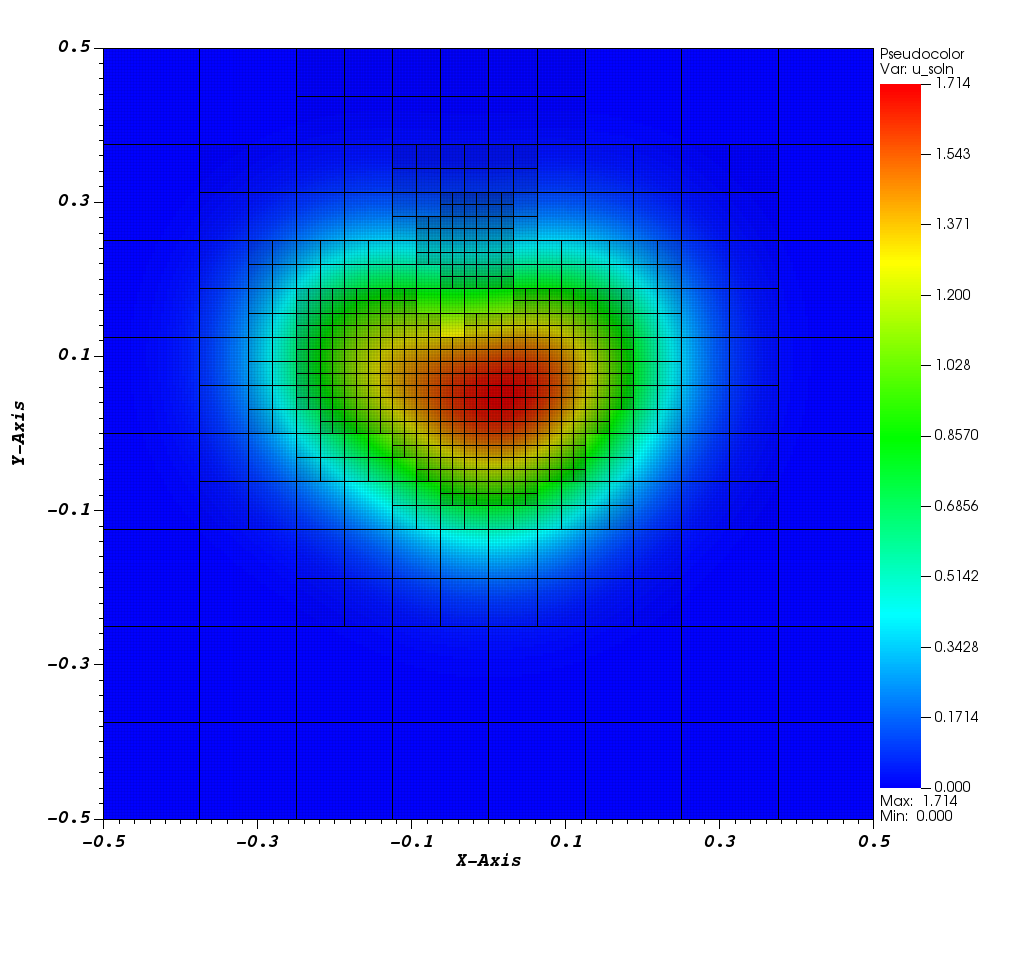
\includegraphics[width=\textwidth]{figures/figure_helmholtz_u.png}
%         \end{subfigure}
%         &
%         \begin{subfigure}[t]{0.3\textwidth}
%             \centering
%             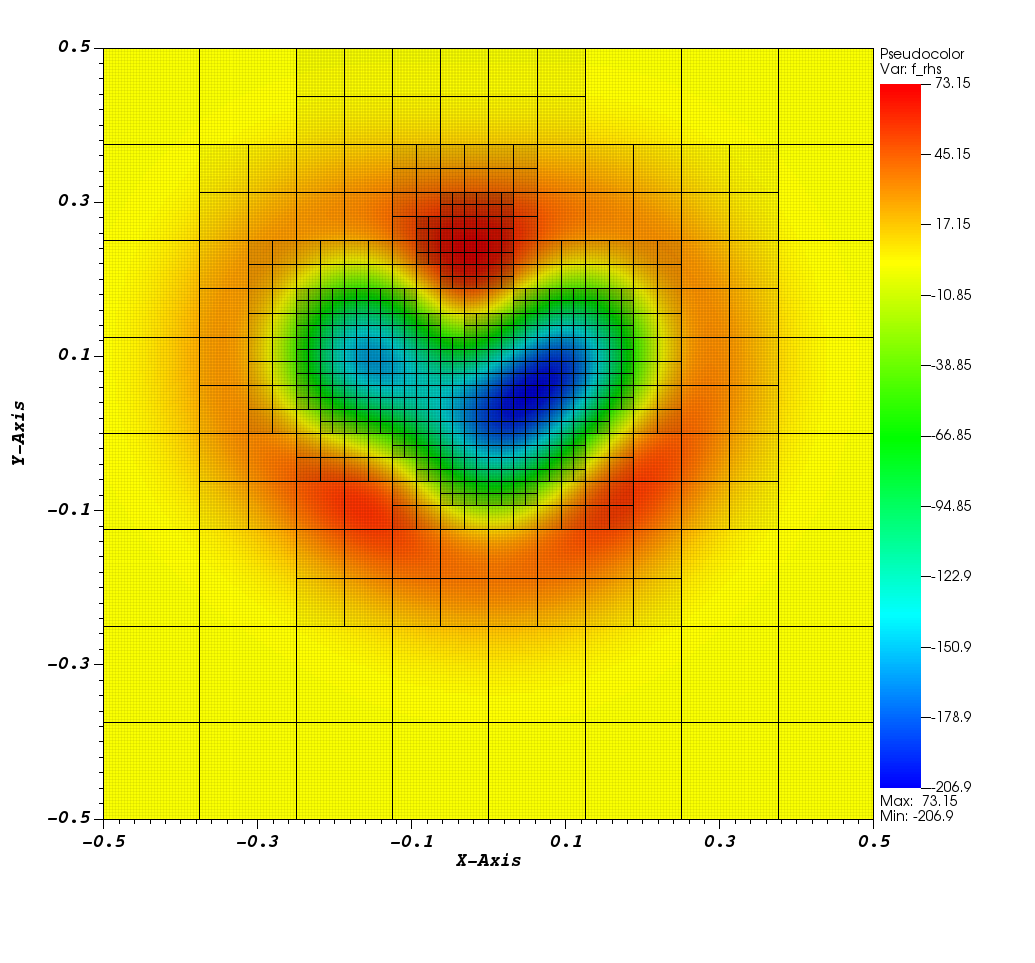
\includegraphics[width=\textwidth]{figures/figure_helmholtz_f.png}
%         \end{subfigure}
%     \end{tabular}
%     \caption{TODO}
%     \label{fig:helmholtz_plots}
% \end{figure}

% \subsection{Laplace's Equation I}

% We solve the following boundary value problem
% \begin{align}
%     \begin{cases}
%         \text{PDE: } & \nabla^2 u(x,y) = 0, (x,y) \in \Omega = [-1, 1] \times [-1 1] \\
%         \text{BC:  } & u(x,y) = g(x,y), (x,y) \in \Gamma = \partial \Omega. \\
%     \end{cases}
%     \label{eqn:laplace}
% \end{align}
% Using a method of manufactured solutions, we compare the numerical solution to an exact solution
% \begin{align}
%     u_{exact}(x,y) = \sin(2 \pi x) \sinh(2 \pi y).
% \end{align}

% \donna{say what $g(x,y)$ is. }

% \donna{It would be great to have a plot here.  Maybe both uniform and adaptive plots?}

% \ignore{As this is a homogeneous problem, there will be no refinement based on the right-hand side.} This acts as an initial test to make sure that the merging and splitting algorithms detailed above are consistent with the order of the patch solver. Using the FISHPACK90 patch solver, we should expect $2^{nd}$ order convergence \citep{adams2016fishpack90}. \donna{Describe the FV discretization.  Fishpack is just a way to solve the resulting linear algebra problem.}

% We solve \ignore{Laplace's equation}  by creating the uniform mesh up to a specified level of refinement $L$. Each patch consists of an $M \times M$ grid of cell-centered points. \donna{Have you described the finite volume discretization?}.  \ignore{The effective resolution $R_{eff}$ is the number of cell-centered points along an entire side of the domain for a uniformly refined mesh.} \ignore{The effective resolution is computed as $R_{eff} = \{\text{Number of patches per side}\} \times \{\text{Number of points per patch}\} = 2^{L+1} \times M$.} We define {\em effective resolution} as $R_{\mbox{eff}}M 2^L$. \donna{Double check this formula.  You probably don't need to spell out in words.}.  For the uniform case, there are several ways to get the same effective resolution. 

% For example, $512 = 8 \times 2^6 = 16 \times 2^5 32 \times 2^4$ and so on. 

% \ignore{For example, on a uniform mesh, to get a $512 \times 512$ resolution, one could use a quadtree with 1 level of refinement (yielding a 2x2 grid of patches) with a patch size of 256x256, or a quadtree with 2 levels of refinement (yielding a 4x4 grid of patches) with a patch size of 128x128, or a quadtree with 3 levels of refinement (yielding an 8x8 grid of patches) with a patch size of 64x64.} 

% \donna{You can,also create an artificial refinement - i.e. refine along diagonals, or something.}

% \subsubsection{Results and Analysis}

% For a given effective resolution, we have observed that the error is essentially independent of the manner in which we achieve the effective resolution.  

%  the same on a uniform grid. Thus, in the subsequent tables, only the effective resolution is shown, despite having run several additional parameter sweeps.  \donna{What do you mean by parameter sweep here?}

% \donna{use siunitx}


% %$ $\begin{center}
% %$ $\sisetup{detect-weight=true,detect-inline-weight=math}
% %$ $\begin{tabular}{
% %$ $   S[table-text-alignment=right]
% %$ $  *2{S[table-column-width=2.25cm,
% %$ $       table-format=2.2e10,
% %$ $       scientific-notation=true,                  
% %$ $       round-mode=places,round-precision=2]}
% %$ $}  % end of column definition
% %$ $\toprule
% %$ $ & \multicolumn{1}{m{2cm}}{\centering Conservation error} &
% %$ $\multicolumn{1}{m{2cm}}{\centering $\infty$-norm error} \\
% %$ $\midrule 
% %$ ${No correction}          & \num{2.4764404912458460e-04} &  \num{1.2338e-01}\\
% %$ ${Fluctuation correction} & \num{2.5302713046460035e-05} &  \num{9.3793e-02}\\
% %$ ${Flux correction}        & \num{2.5111614390205261e-04} &  \num{1.2293e-01}\\
% %$ ${All corrections}        & \num{0.0000000000000000e+00} &  \num{9.5006e-02}\\
% %$ $\bottomrule
% %$ $\end{tabular}
% %$ $\end{center}
% %$ $\label{tab:conservation_cubedsphere}
% %$ $\end{table}

% % Table generated by Excel2LaTeX from sheet 'laplace-1'
% \begin{table}[htbp]
%     \centering
%     \caption{Convergence and Timing for the Laplace I Problem. The columns show the effective resolution $R_{eff}$, the $L_1$ error computed from the exact solution, the order of convergence, timing for the build $T_{build}$ and solve $T_{solve}$ stages, and the required memory $S$ to store the factorization. The data show expected second order convergence.   \donna{Is data for a fixed patch size? Add a column for the level used.}}
%     \begin{tabular}{|r|r|r|r|r|r|}
%         \toprule
%         \multicolumn{1}{|l|}{$R_{eff}$} & \multicolumn{1}{l|}{$L_1$ Error} & \multicolumn{1}{l|}{Order} & \multicolumn{1}{l|}{$T_{build}$ (sec)} & \multicolumn{1}{l|}{$T_{solve}$ (sec)} & \multicolumn{1}{l|}{S (MB)} \\
%         \midrule
%         \midrule
%         8     & 3.0580E+00 &       & 2.3421E-04 & 1.0308E-03 & 9.2936E-03 \\
%         16    & 1.0991E+00 & 1.4762E+00 & 1.0122E-03 & 9.1642E-04 & 3.6149E-02 \\
%         32    & 3.0879E-01 & 1.8317E+00 & 7.6679E-03 & 5.4845E-03 & 1.4259E-01 \\
%         64    & 7.9664E-02 & 1.9546E+00 & 5.4575E-02 & 1.8398E-02 & 5.6642E-01 \\
%         128   & 2.0097E-02 & 1.9869E+00 & 4.6770E-01 & 5.7012E-02 & 2.2578E+00 \\
%         256   & 5.0345E-03 & 1.9971E+00 & 2.1628E+00 & 2.1096E-01 & 2.7051E+01 \\
%         512   & 1.2594E-03 & 1.9991E+00 & 9.8592E+00 & 9.1265E-01 & 1.8024E+02 \\
%         1024  & 3.1488E-04 & 1.9998E+00 & 4.4384E+01 & 3.9901E+00 & 1.0090E+03 \\
%         2048  & 7.8723E-05 & 2.0000E+00 & 1.9991E+02 & 1.8425E+01 & 5.1883E+03 \\
%         \bottomrule
%     \end{tabular}%
%     \label{tab:laplace-1}%
% \end{table}%

% \donna{Try with more levels. }


% As \reftab{tab:laplace-1} shows, our current implementations shows the expected second order convergence.   The merging and splitting algorithms detailed in this paper are consistent with the order of the patch solver. \donna{These results are consistent with the results shown in M and G.  The linear algebra involved in merging and splitting does not causes errors to propagate}.  The timing for the build and solve stages grow as the resolution grows. Storage for the set of solution operators also grows as the resolution increases. 

% Direct methods tend to be more storage intensive than iterative methods. The adaptive implementation will help decrease the memory requirements for the HPS method. \donna{This is a better statement for the conclusions, since it is a very general statement. }

% \subsection{Poisson's Equation I}

% We solve the following boundary value problem
% \begin{align}
%     \begin{cases}
%         \text{PDE: } & \nabla^2 u(x,y) = f(x,y), (x,y) \in \Omega = [-1, 1] \times [-1 1] \\
%         \text{BC:  } & u(x,y) = g(x,y), (x,y) \in \Gamma = \partial \Omega. \\
%     \end{cases}
% \end{align}
% with a manufactured exact solution of
% \begin{align}
%     u_{exact}(x,y) &= \sin(c \pi x) + \cos(c \pi y) \\
%     f(x,y) &= -(c \pi)^2 u(x,y).
% \end{align}
% We use $c = 2$ for this case.

% With an inhomogeneous right-hand side, we can adapt the mesh according to the load function $f$. Where $|f(x,y)|$ is large, the curvature of the solution is large. Thus, we refine according to $|f(x,y)| > \epsilon$, with $\epsilon = 50$ for this case.

% \subsubsection{Results and Analysis}

% The results of this convergence study are shown in \reftab{tab:poisson-1}. As in the first example, we report the error with increasing effective resolution. The upwards time reported in \reftab{tab:poisson-1} shows the time required for the upwards pass needed with a non-homogeneous elliptic problem as outlined in \refsec{subsub:4to1-upwards}.

% % Table generated by Excel2LaTeX from sheet 'poisson-1'
% \begin{table}[htbp]
%     \centering
%     \begin{tabular}{|r|r|r|r|r|r|}
%         \toprule
%         \multicolumn{1}{|l|}{$R_{eff}$} & \multicolumn{1}{l|}{$L_{1}$ Error} & \multicolumn{1}{l|}{Order} & \multicolumn{1}{l|}{$T_{build}$ (sec)} & \multicolumn{1}{l|}{$T_{upwards}$ (sec)} & \multicolumn{1}{l|}{$T_{solve}$ (sec)} \\
%         \midrule
%         64    & 2.55E-03 &       & 5.41E-02 & 7.19E-03 & 2.46E-02 \\
%         128   & 6.36E-04 & 2.00E+00 & 2.77E-01 & 5.60E-02 & 7.04E-02 \\
%         256   & 1.59E-04 & 2.00E+00 & 1.49E+00 & 2.95E-01 & 2.26E-01 \\
%         512   & 7.37E-05 & 1.11E+00 & 3.52E+00 & 5.58E-01 & 2.87E-01 \\
%         1024  & 1.86E-05 & 1.99E+00 & 1.60E+01 & 3.26E+00 & 1.24E+00 \\
%         \midrule
%         128   & 6.36E-04 &       & 2.98E-01 & 2.95E-02 & 5.12E-02 \\
%         256   & 1.59E-04 & 2.00E+00 & 1.51E+00 & 2.15E-01 & 2.11E-01 \\
%         512   & 3.97E-05 & 2.00E+00 & 7.29E+00 & 1.11E+00 & 9.49E-01 \\
%         1024  & 1.86E-05 & 1.09E+00 & 1.60E+01 & 2.05E+00 & 1.18E+00 \\
%         2048  & 4.67E-06 & 1.99E+00 & 7.58E+01 & 1.16E+01 & 5.44E+00 \\
%         \bottomrule
%     \end{tabular}%
%     \caption{Convergence and Timing for the Poisson I Problem. The columns report the effective resolution $R_{eff}$, the $L_1$ error, the order of convergence, and the timing for the build $T_{build}$, upwards $T_{upwards}$, and $T_{solve}$ stages.}
%     \label{tab:poisson-1}%
% \end{table}%  

% This numerical experiment shows that even with an adaptive scheme, we maintain the expected $2^{nd}$ order convergence. The timing for the build and solve stages is also faster than the build and solve stages of the Laplace example, almost by an order of magnitude.

% \subsection{Poisson's Equation II}

% As another test for Poisson's equation, we solve a ``polar star'' Poisson problem. The problem is created via a method of manufactured solutions and is engineered to have highly local curvature from the load function. The resulting solution is a collection of polar stars with user specified number of points and radii of curvature. This problem highlights the use of an adaptive mesh to solve the elliptic equation. The exact solution we attempt to reconstruct is the following:
% \begin{align}
%     u(x,y) = \frac{1}{2} \sum_{i=1}^{N} 1 - \tanh \left(\frac{r(x,y)-r_{0,i} \left(r_{1,i} \cos \left(n \theta(x,y)\right)+1\right)}{\epsilon }\right)
% \end{align}
% % Details on the right-hand side and parameters can be found in Appendix \ref{apdx:polar_star_problem}.
% Computing the Laplacian analytically yields the right-hand side to Poisson's equation. Thus, the polar star Poisson problem is defined as follows:
% \begin{align}
%     \nabla^2 u(x,y) = \sum_{i=1}^N -\frac{s_{1,i}(x,y) + s_{2,i}(x, y)}{r(x,y)^2} - s_{3,i}(x,y) + s_{4,i}(x,y)
% \end{align}
% with
% \begin{align*}
%     s_{1,i}(x,y) &= \frac{p(x,y)^2 \tanh \left(\phi(x,y)\right) \text{sech}^2\left(\phi(x,y)\right)}{\epsilon ^2} \\
%     s_{2,i}(x,y) &= -\frac{n^2 r_{0,i} r_{1,i} \cos (n \theta(x,y)) \text{sech}^2\left(\phi(x,y)\right)}{2 \epsilon } \\
%     s_{3,i}(x,y) &= \frac{\tanh \left(\phi(x,y)\right) \text{sech}^2\left(\phi(x,y)\right)}{\epsilon ^2} \\
%     s_{4,i}(x,y) &= \frac{\text{sech}^2\left(\phi(x,y)\right)}{2 r(x,y) \epsilon } \\
%     p(x,y) &= n r_{0,i} r_{1,i} \sin (n \theta(x,y)) \\
%     \phi(x,y) &= \frac{r(x,y)-r_{0,i} (r_{1,i} \cos (n \theta(x,y))+1)}{\epsilon}
% \end{align*}
% and where $i=1, ..., N_{polar}$ and $N_{polar}$ is the number of polar stars. Each polar star has a center $(x_0, y_0)$, inner and outer radii $r_0, r_1$, and the number of arms per polar star $n$. The radius and angle have the standard polar transforms:
% \begin{align}
%     r(x,y) &= \sqrt{(x - x_0)^2 + (y - y_0)^2} \\
%     \theta(x,y) &= \tan^{-1}\Big(\frac{y - y_0}{x - x_0}\Big)
% \end{align}
% \reftab{table:polar_star_parameters} has the parameters used in this case study.
% \begin{table}[h]
%     \begin{center}
%         \begin{tabular}{|c|c|c|c|c|c|}
%             \hline
%             $i$ & $x_0$ & $y_0$ & $r_0$ & $r_1$ & $n$ \\
%             \hline
%             $1$ & $-0.5$ & $-0.5$ & $0.1$ & $0.2$ & $4$ \\
%             $2$ & $0.5$ & $0.5$ & $0.1$ & $0.2$ & $7$ \\
%             \hline
%         \end{tabular}
%         \caption{Polar Star Poisson Problem Parameters}
%         \label{table:polar_star_parameters}
%     \end{center}
% \end{table}

% % \begin{figure}
% %     \centering
% %     \begin{tabular}{c c}
% %         \begin{subfigure}[t]{0.45\textwidth}
% %             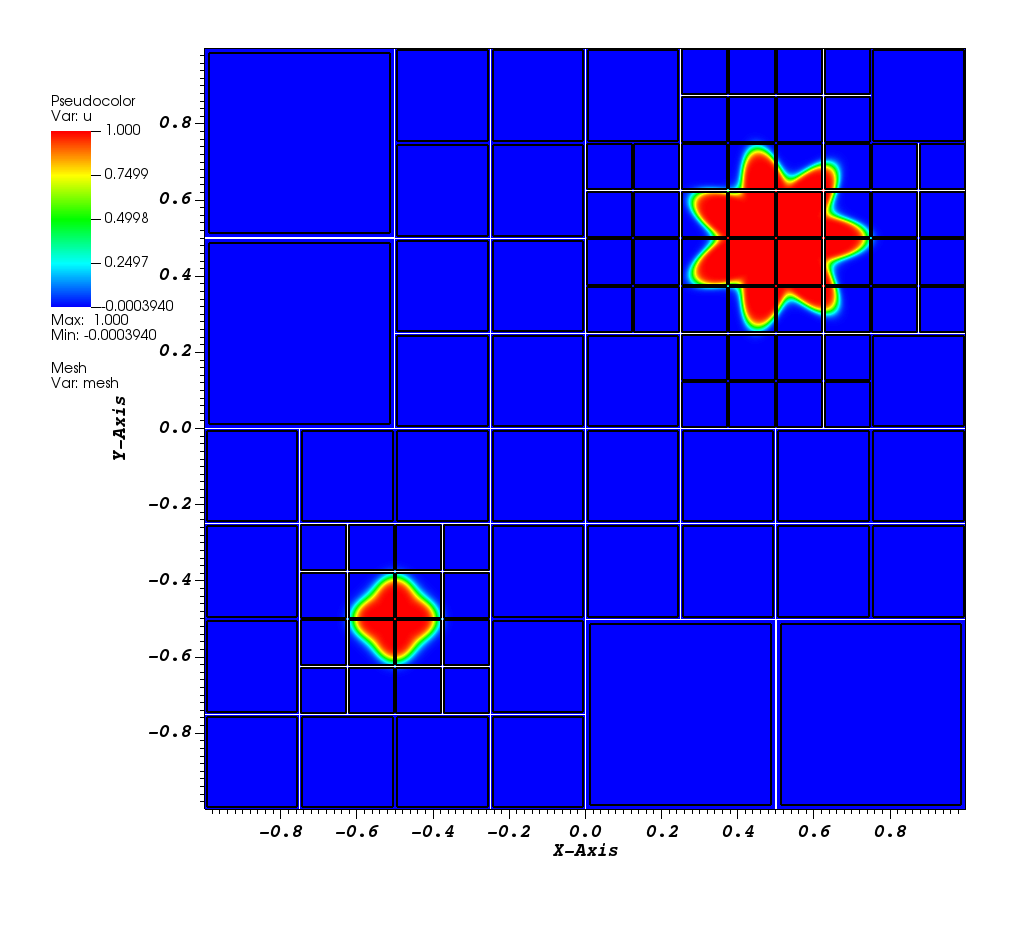
\includegraphics[width=\textwidth]{figures/poisson_2d_solution0000.png}
% %             \caption{Solution}
% %         \end{subfigure}
% %         &
% %         \begin{subfigure}[t]{0.45\textwidth}
% %             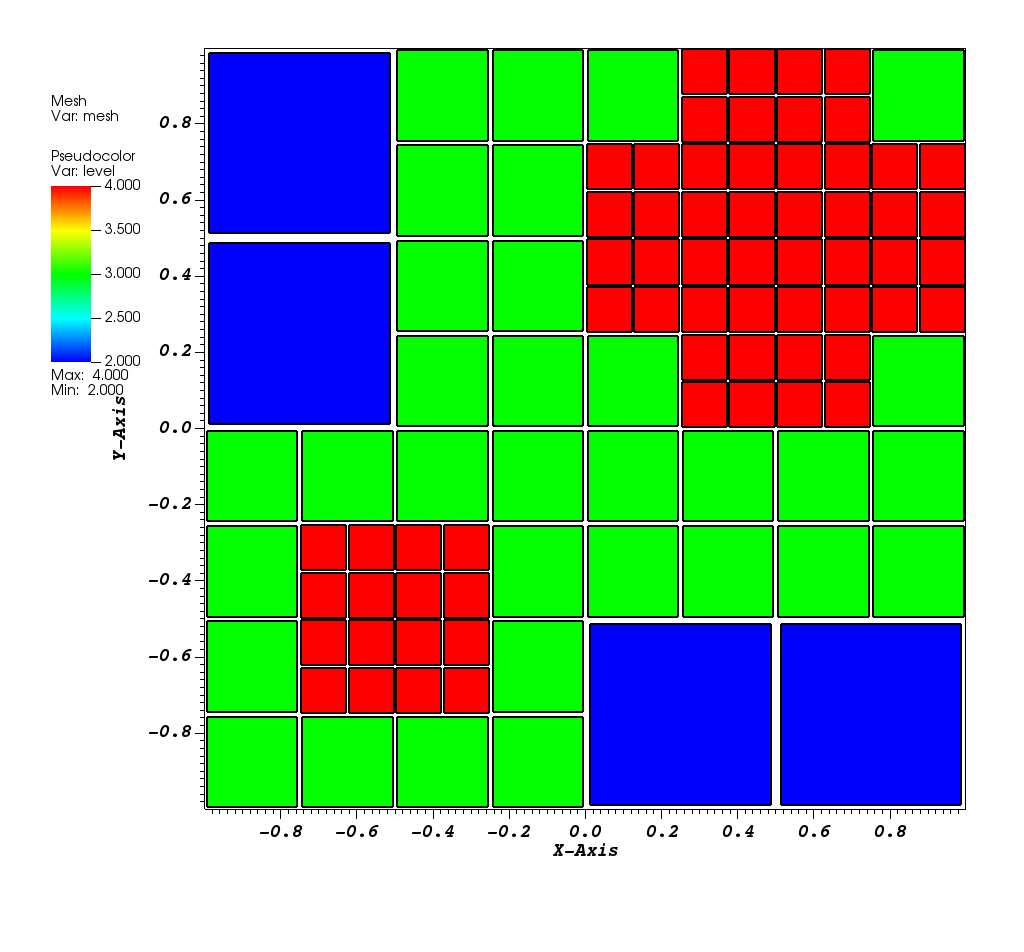
\includegraphics[width=\textwidth]{figures/poisson_levels0000.png}
% %             \caption{Mesh colored by refinement level}
% %         \end{subfigure}
% %     \end{tabular}
% %     \caption{The solution and mesh for the polar star Poisson problem.}
% %     \label{solution_and_mesh_polar_star}
% % \end{figure}

% \subsubsection{Results and Analysis}

% To run a convergence analysis, we solve the polar star Poisson problem on both uniform and adaptive meshes at various resolutions with different patch sizes.

% % Table generated by Excel2LaTeX from sheet 'poisson-2-prev'
% \begin{table}[htbp]
%     \centering
%     \begin{tabular}{|c|c|c|r|r|r|r|r|}
%         \toprule
%         \multicolumn{1}{|l|}{$M$} & \multicolumn{1}{l|}{Mode} & \multicolumn{1}{l|}{$L_{max}$} & \multicolumn{1}{l|}{$R_{eff}$} & \multicolumn{1}{l|}{$N_{DOF}$} & \multicolumn{1}{l|}{$L_1$ Error} & \multicolumn{1}{l|}{Ratio} & \multicolumn{1}{l|}{S (MB)} \\
%         \midrule
%         \midrule
%         \multirow{8}[4]{*}{32} & \multirow{4}[2]{*}{Uniform} & 1     & 64    & 4096  & 1.9397E+00 &       & 1.7003 \\
%         &       & 2     & 128   & 16384 & 4.6616E-01 &       & 11.3109 \\
%         &       & 3     & 256   & 65536 & 2.7698E-02 &       & 63.2631 \\
%         &       & 4     & 512   & 262144 & 1.4022E-04 &       & 325.0915 \\
%         \cmidrule{2-8}          & \multirow{4}[2]{*}{Adaptive} & 1     & 64    & 4096  & 1.9397E+00 & 1.00  & 1.7003 \\
%         &       & 2     & 128   & 10240 & 4.6615E-01 & 0.63  & 4.0637 \\
%         &       & 3     & 256   & 40960 & 2.7698E-02 & 0.63  & 27.5282 \\
%         &       & 4     & 512   & 102400 & 1.3903E-04 & 0.39  & 51.1623 \\
%         \midrule
%         \multirow{8}[4]{*}{64} & \multirow{4}[2]{*}{Uniform} & 1     & 128   & 16384 & 4.6616E-01 &       & 6.7755 \\
%         &       & 2     & 256   & 65536 & 2.7698E-02 &       & 45.1214 \\
%         &       & 3     & 512   & 262144 & 1.4022E-04 &       & 252.5248 \\
%         &       & 4     & 1024  & 1048576 & 2.1169E-05 &       & 1298.1774 \\
%         \cmidrule{2-8}          & \multirow{4}[2]{*}{Adaptive} & 1     & 128   & 16384 & 4.6616E-01 & 1.00  & 6.7755 \\
%         &       & 2     & 256   & 40960 & 2.7698E-02 & 0.63  & 16.1897 \\
%         &       & 3     & 512   & 163840 & 1.4022E-04 & 0.63  & 109.8055 \\
%         &       & 4     & 1024  & 409600 & 2.2336E-05 & 0.39  & 203.9475 \\
%         \midrule
%         \multirow{8}[4]{*}{128} & \multirow{4}[2]{*}{Uniform} & 1     & 256   & 65536 & 2.7698E-02 &       & 27.0509 \\
%         &       & 2     & 512   & 262144 & 1.4022E-04 &       & 180.2425 \\
%         &       & 3     & 1024  & 1048576 & 2.1169E-05 &       & 1009.0483 \\
%         &       & 4     & 2048  & 4194304 & 5.3546E-06 &       & 5188.3493 \\
%         \cmidrule{2-8}          & \multirow{4}[2]{*}{Adaptive} & 1     & 256   & 65536 & 2.7698E-02 & 1.00  & 27.0509 \\
%         &       & 2     & 512   & 163840 & 1.4022E-04 & 0.63  & 64.6291 \\
%         &       & 3     & 1024  & 655360 & 2.1169E-05 & 0.63  & 438.6102 \\
%         &       & 4     & 2048  & 1638400 & 5.6348E-06 & 0.39  & 814.3928 \\
%         \bottomrule
%     \end{tabular}%
%     \caption{Convergence Results for the Poisson II Problem. The columns report the patch size $M$, the mode of mesh generation (uniform or adaptive), the maximum level of refinement $L_{max}$, the total degrees of freedom $N_{DOF}$, the ratio between adaptive and uniform degrees of freedom, and the size $S$ in MB to store the associated data.}
%     \label{tab:poisson-2}%
% \end{table}%

% Figures \ref{plot:timing} and \ref{plot:work_precision} contain resolution vs. timing and timing vs. error (work-precision) plots for the polar-star Poisson problem. Each plot shows results for the build, upwards, and solve stages of the quadtree-adaptive HPS method.

% In \reffig{plot:timing}, the timing for each of the stages is given for various patch sizes and resolutions for both the uniform and adaptive cases. We observe good scaling of the build stage, consistent with the $\mathcal{O}^{3/2}$ scaling of the HPS method. The upwards stage is about an order of magnitude faster than the build stage, and the solve stage is an additional order of magnitude faster. In a transient implementation of this method on a static mesh, the overhead associated with the build stage is outweighed by the time saving of a very fast solve stage each time step. Also note that improvements in timing when using an adaptive scheme. This is shown more in the work-precision plots of \reffig{plot:work_precision}. For the same error, the adaptive implementation can solve the problem $20\%-50\%$ faster.

% \begin{figure}[htbp]
%     \centering
%     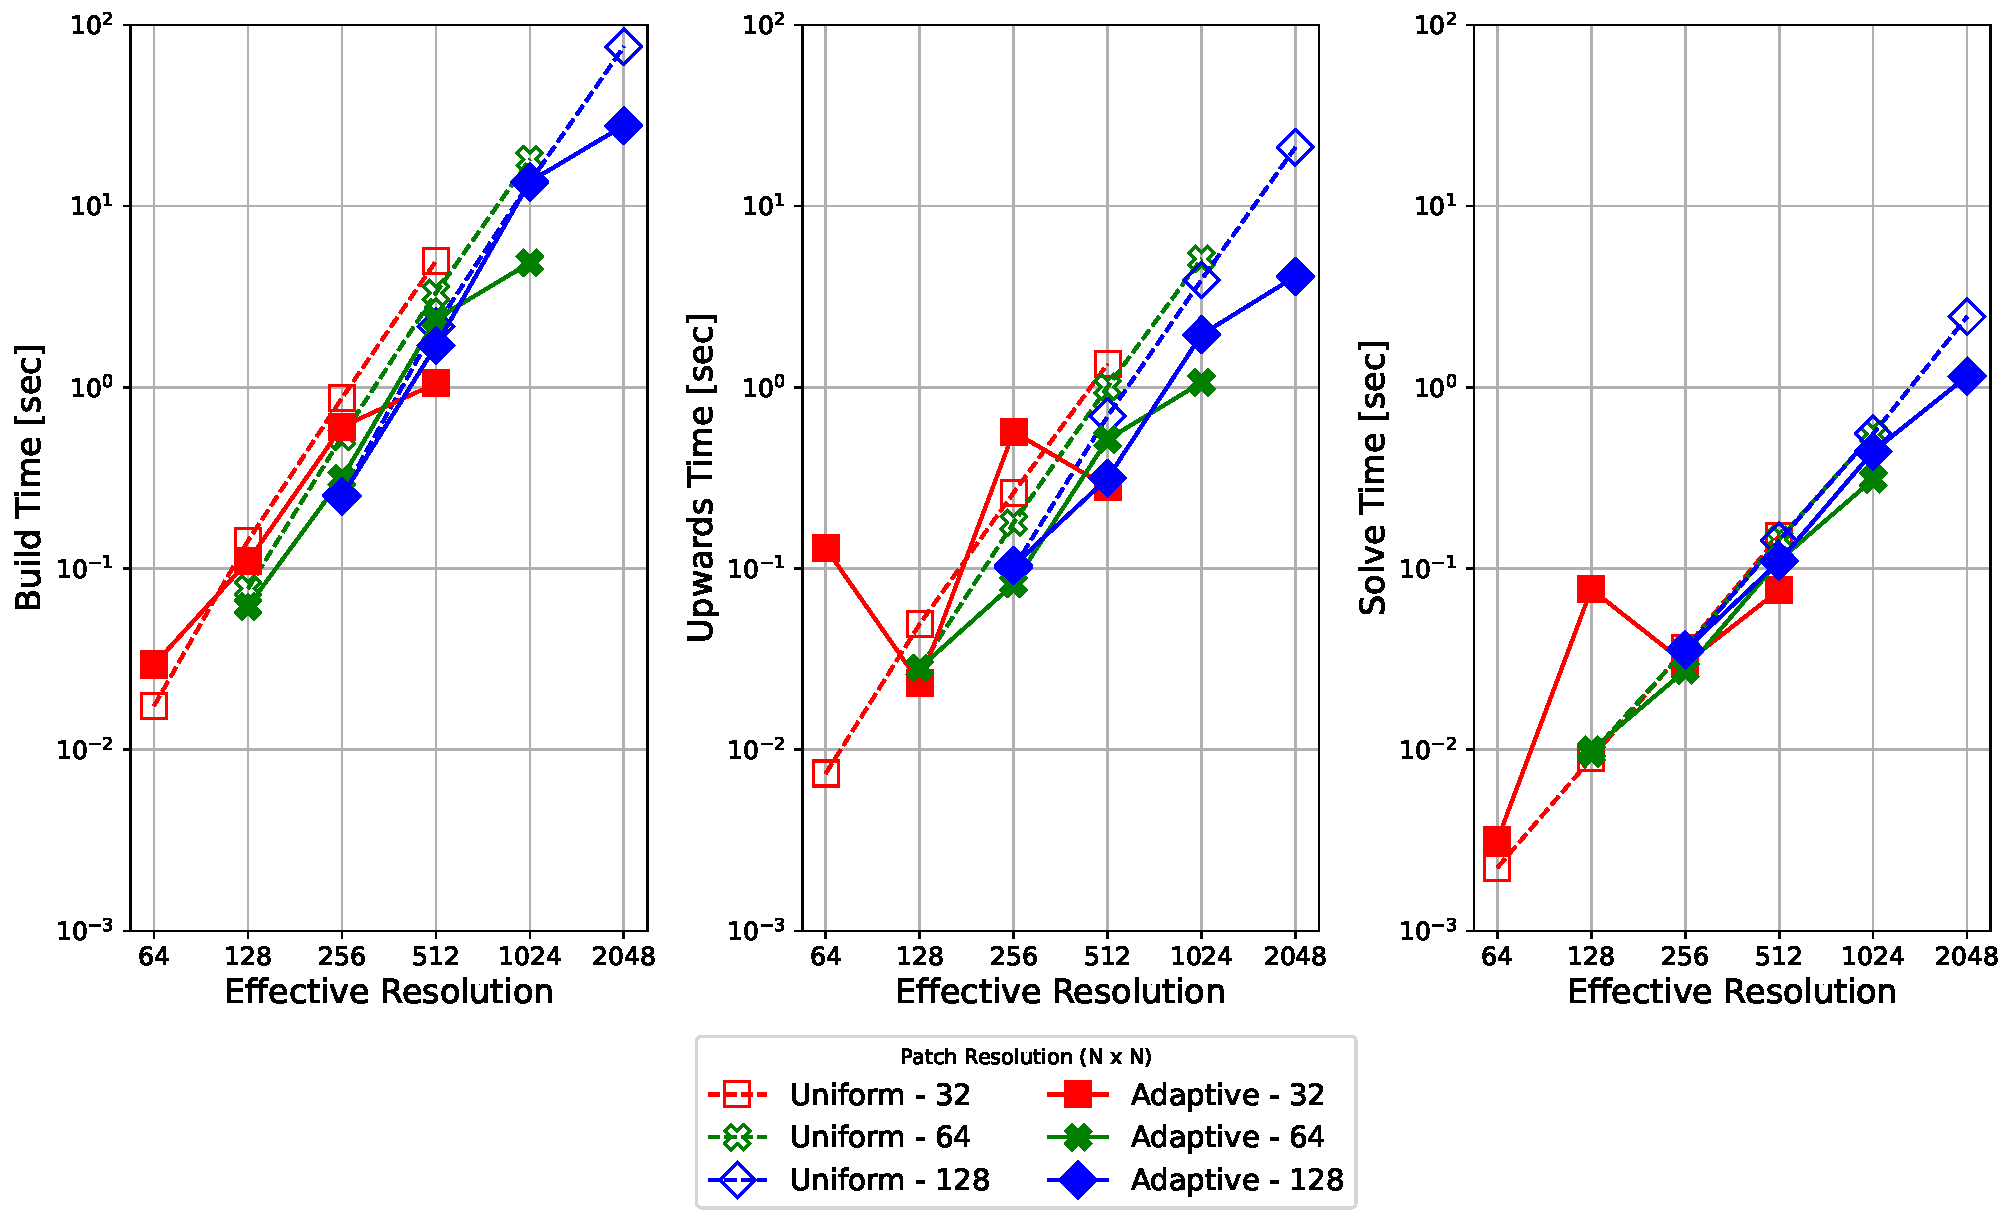
\includegraphics[width=1.0\textwidth]{figures/plot_timing.pdf}
%     \caption{Timing Plots for the Polar-Star Poisson Problem}
%     \label{plot:timing}
% \end{figure}

% \begin{figure}[htbp]
%     \centering
%     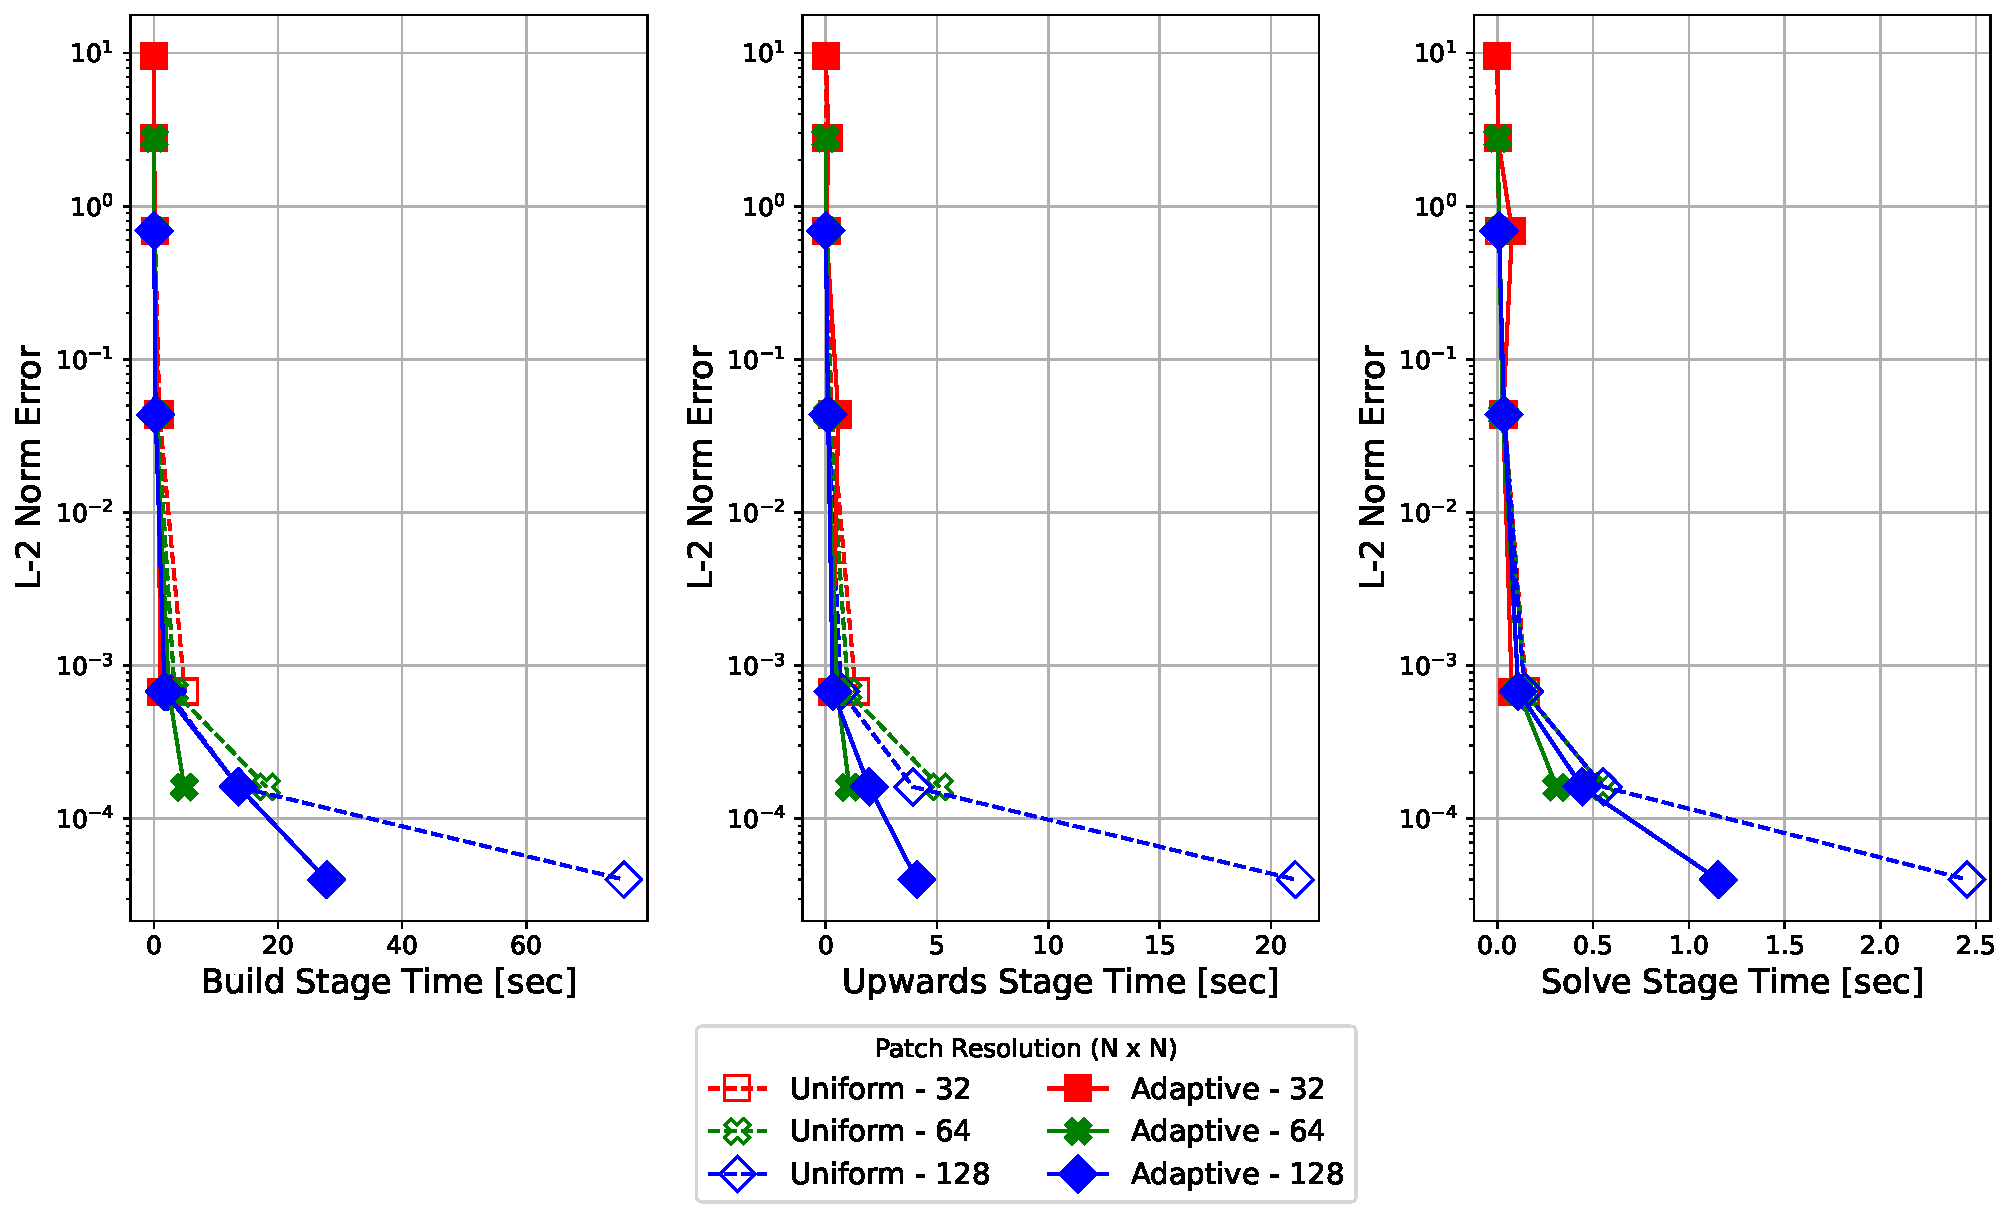
\includegraphics[width=1.0\textwidth]{figures/plot_work_precision.pdf}
%     \caption{Work-Precision Plots for the Polar-Star Poisson Problem}
%     \label{plot:work_precision}
% \end{figure}

% \subsection{Helmholtz's Equation II}

% We now solve the following Helmholtz equation:
% \begin{align}
%     \begin{cases}
%         \text{PDE: } & \nabla^2 u(x,y) + \kappa^2 u(x,y) = 0, (x,y) \in \Omega = [-1, 1] \times [-1 1] \\
%         \text{BC:  } & u(x,y) = g(x,y), (x,y) \in \Gamma = \partial \Omega. \\
%     \end{cases}
% \end{align}
% To provide an exact solution to compare to, we use a manufactured exact solution of
% \begin{align}
%     u_{exact}(x,y) = Y_0(\kappa r(x,y))
% \end{align}
% where $Y_0$ is the zeroth Bessel function of the second kind, $\kappa$ is related to the wavelength $\lambda = \frac{2 \pi}{\kappa}$, and $r(x,y) = \sqrt{(x - x_0)^2 + (y - y_0)^2}$ is the distance from the singularity of the Bessel function. This represents a vibration problem on the domain and is the same problem used in \citep{gillman2014direct} to test their implementation. We use $x_0 = -2, y_0 = 0$ and vary $\kappa$ (as detailed in \reftab{tab:helmholtz-1}).

% A Helmholtz equation with a high wave number suffers from the so-called ``pollution problem''. A high wave number corresponds to a highly oscillatory solution that is difficult to be captured with lower mesh resolutions. To ensure our implementation works for decently large wave numbers, we run a convergence study with varying values of $\kappa$ and check convergence. For more details on the pollution problem, see \citep{peterseim2017eliminating} or \citep{dwarka2021pollution}.

% {\bf Results and Analysis}
% \reftab{tab:helmholtz-1} contains the convergence study and parameter sweep for $\kappa$. We vary $\kappa$ and vary the level of refinement and patch size to get various effective resolutions. The values of the wave number $\kappa$ correspond to values of the wavelength $\lambda$ that vary across three orders of magnitude.

% % Table generated by Excel2LaTeX from sheet 'helmholtz-1'
% \begin{table}[htbp]
%     \centering
%     \begin{tabular}{|c|r|r|r|r|r|r|}
%         \toprule
%         \multicolumn{1}{|l|}{$\kappa$} & \multicolumn{1}{l|}{$R_{eff}$} & \multicolumn{1}{l|}{$L_1$ Error} & \multicolumn{1}{l|}{Order} & \multicolumn{1}{l|}{$T_{build}$ (sec)} & \multicolumn{1}{l|}{$T_{solve}$ (sec)} & \multicolumn{1}{l|}{$S$ (MB)} \\
%         \midrule
%         \midrule
%         \multirow{4}[2]{*}{1} & 256   & 2.24E-06 &       & 7.62E-01 & 2.33E-01 & 2.71E+01 \\
%         & 512   & 5.60E-07 & 2.00E+00 & 2.99E+00 & 9.49E-01 & 1.80E+02 \\
%         & 1024  & 1.40E-07 & 2.00E+00 & 1.81E+01 & 4.00E+00 & 1.01E+03 \\
%         & 2048  & 3.50E-08 & 2.00E+00 & 8.68E+01 & 1.84E+01 & 5.19E+03 \\
%         \midrule
%         \multirow{4}[2]{*}{10} & 256   & 3.28E-04 &       & 7.58E-01 & 2.13E-01 & 2.71E+01 \\
%         & 512   & 8.20E-05 & 2.00E+00 & 2.98E+00 & 9.48E-01 & 1.80E+02 \\
%         & 1024  & 2.05E-05 & 2.00E+00 & 1.59E+01 & 4.30E+00 & 1.01E+03 \\
%         & 2048  & 5.13E-06 & 2.00E+00 & 8.61E+01 & 1.78E+01 & 5.19E+03 \\
%         \midrule
%         \multirow{4}[2]{*}{20} & 256   & 2.58E-03 &       & 7.58E-01 & 2.02E-01 & 2.71E+01 \\
%         & 512   & 8.84E-04 & 1.54E+00 & 2.95E+00 & 9.60E-01 & 1.80E+02 \\
%         & 1024  & 2.61E-04 & 1.76E+00 & 1.58E+01 & 3.93E+00 & 1.01E+03 \\
%         & 2048  & 6.86E-05 & 1.93E+00 & 8.94E+01 & 1.81E+01 & 5.19E+03 \\
%         \midrule
%         \multirow{4}[2]{*}{30} & 256   & 7.89E-03 &       & 7.81E-01 & 2.15E-01 & 2.71E+01 \\
%         & 512   & 1.60E-02 & -1.02E+00 & 2.97E+00 & 9.62E-01 & 1.80E+02 \\
%         & 1024  & 8.08E-04 & 4.31E+00 & 1.59E+01 & 3.97E+00 & 1.01E+03 \\
%         & 2048  & 1.76E-04 & 2.20E+00 & 8.49E+01 & 1.83E+01 & 5.19E+03 \\
%         \midrule
%         \multirow{4}[2]{*}{40} & 256   & 2.72E-02 &       & 7.85E-01 & 2.96E-01 & 2.71E+01 \\
%         & 512   & 1.10E-02 & 1.31E+00 & 2.98E+00 & 9.38E-01 & 1.80E+02 \\
%         & 1024  & 1.00E-03 & 3.46E+00 & 1.61E+01 & 4.01E+00 & 1.01E+03 \\
%         & 2048  & 2.31E-04 & 2.11E+00 & 8.46E+01 & 1.83E+01 & 5.19E+03 \\
%         \bottomrule
%     \end{tabular}%
%     \caption{Convergence Study with Increasing Values of $\kappa$. The columns report the value of the wave number $\kappa$, the effective resolution $R_{eff}$, the $L_1$ error, the order of convergence, the timing for the build $T_{build}$ and solve $T_{solve}$ stages, and the memory storage $S$ for the associated data.}
%     \label{tab:helmholtz-1}%
% \end{table}%

% For each value of $\kappa$, we report the expected $2^{nd}$ order convergence. However, for larger values of $\kappa$, the actual error is lower and lower. This is to be expected at the resolutions we have run our study at. For larger and larger values of $\kappa$, even more resolution would be needed to better capture the smaller and smaller wavelengths. The timing results for this problem are consistent with the times reported in the other problems.

% \subsection{Heat Equation I}

% The time-dependent heat equation can be solved with an elliptic solver as implemented in this paper using a backward Euler time stepping scheme. The heat equation is given as
% \begin{align}
%     \frac{\partial u(x,y,t)}{\partial t} &= \nabla^2 u(x,y,t)
% \end{align}
% for $(x,y) \in \Omega$ and $t \in [0, \infty)$. Applying a backward Euler scheme results in the following:
% \begin{align}
%     \nabla^2 u^{n+1} - \lambda u^{n+1} = -\lambda u^{n}
% \end{align}
% with $\lambda = -\frac{1}{\Delta t}$. This results in a Helmholtz-like equation that we can solve with our implemented HPS method. The advantage to using this scheme is we can perform the build stage prior to any time stepping, then do the upwards and solve stages each time step to perform the update. This results in a very fast and efficient scheme for time-dependent problems. Each time step, the right-hand side is updated with the solution at the previous time step.

% For initial conditions, we will use $u_{exact} = u_0(x,y)$ from the Poisson I test problem. We work on a square domain $\Omega = [0, 1] \times [0, 1]$, with homogeneous, Dirichlet boundary conditions. The analytical solution to this problem can be found via separation of variables and provides an exact solution to compare to. The analytical solution is
% \begin{align}
%     u_{exact}(x,y,t) = \sum_{m=1}^{\infty} \sum_{n=1}^{\infty} A_{mn} \sin(k_x x) \sin(k_y y) e^{-(k_x^2 + k_y^2) t}
% \end{align}
% where $k_x = m \pi$, $k_y = n \pi$, and
% \begin{align}
%     A_{mn} = 4 \int_0^1 \int_0^1 u_0(x,y) \sin(k_x x) \sin(k_y y) dy dx
% \end{align}

% \subsubsection{Results and Analysis}

% \reftab{tab:heat-1} contains the results of solving the heat equation from $t = 0$ to $t = 0.01$. This time was chosen to have the solution not decay entirely in order to check for correctness. This problem was run on a grid with an effective resolution of $512 \times 512$, or $L_{max} = 4$ and $M = 32$. The error more or less remains constant during the simulation. Once the initial build stage is done, each subsequent time step requires one upward pass and one downward pass in the solve stage, resulting in very fast time-to-solutions for the effective resolution. The memory required to store the set of solution operators remains constant throughout the entire run.

% % Table generated by Excel2LaTeX from sheet 'heat-1'
% \begin{table}[htbp]
%     \centering
%     \begin{tabular}{|r|r|r|r|r|r|}
%         \toprule
%         \multicolumn{1}{|l|}{Time (sec)} & \multicolumn{1}{l|}{$L_1$ Error} & \multicolumn{1}{l|}{$T_{build}$ (sec)} & \multicolumn{1}{l|}{$T_{upwards}$ (sec)} & \multicolumn{1}{l|}{$T_{solve}$ (sec)} & \multicolumn{1}{l|}{$S$ (MB)} \\
%         \midrule
%         \midrule
%         0.00E+00 & 7.81E-01 & 5.59E+00 & 1.49E+00 & 9.43E-01 & 3.25E+02 \\
%         1.11E-03 & 4.63E-01 & 0.00E+00 & 1.50E+00 & 1.00E+00 & 3.25E+02 \\
%         2.22E-03 & 2.98E-01 & 0.00E+00 & 1.47E+00 & 9.53E-01 & 3.25E+02 \\
%         3.33E-03 & 2.00E-01 & 0.00E+00 & 1.49E+00 & 1.02E+00 & 3.25E+02 \\
%         4.44E-03 & 1.38E-01 & 0.00E+00 & 1.67E+00 & 9.86E-01 & 3.25E+02 \\
%         5.56E-03 & 9.83E-02 & 0.00E+00 & 1.49E+00 & 9.89E-01 & 3.25E+02 \\
%         6.67E-03 & 7.24E-02 & 0.00E+00 & 1.51E+00 & 9.64E-01 & 3.25E+02 \\
%         7.78E-03 & 5.54E-02 & 0.00E+00 & 1.47E+00 & 9.38E-01 & 3.25E+02 \\
%         8.89E-03 & 4.41E-02 & 0.00E+00 & 1.51E+00 & 9.90E-01 & 3.25E+02 \\
%         1.00E-02 & 3.64E-02 & 0.00E+00 & 1.49E+00 & 9.77E-01 & 3.25E+02 \\
%         \bottomrule
%     \end{tabular}%
%     \caption{Error and Timing Results for the Heat Equation. The columns report the simulation time, the $L_1$ error, the time for the build $T_{build}$, upwards $T_{upwards}$, and solve $T_{solve}$ stages, and the memory requirements $S$ to store the associated data. Note that the only time the build stage (matrix factorization) is called is for the first time step. All future time steps consist of just the upwards pass and the application of the set of solution operators.}
%     \label{tab:heat-1}%
% \end{table}%
\section{Conclusion}

The work presented in this paper demonstrates a successful implementation of the quadtree-adaptive Hierarchical Poincaré-Steklov (HPS) method in parallel. The integration of the \pforest\ library, known for its efficiency and scalability, with the communication patterns of the quadtree-adaptive HPS method, shows promise for an effective solver for elliptic PDEs. As distributed memory architectures are increasingly more common in commodity clusters, an MPI implementation is essential for future scalability.

Running strong and weak scaling analysis on Polaris, one of the world's top 50 fastest supercomputers, provides insights into potential and necessary improvements for further optimizations. The current bottleneck is the communication required for the family callbacks during family traversals of the path-indexed quadtree. Potential optimizations include reducing redundant calculations through more efficient matrix partitioning and investigating non-blocking communication to better overlap compute and communication. These insights are currently being investigated and integrated into EllipticForest \citep{chipman2024ellipticforest}.

\chapter{An Adaptive Rebuild Technique for the Quadtree-Adaptive HPS Method}
\label{chap:adaptive-build}
\section{Introduction}
\label{sec:intro}

The \gls{qahps} method is a direct method for solving elliptic \gls{pdes} on a hierarchy of adaptively refined finite volume meshes. It builds upon the \gls{hps} methods first presented by \citet{gillman2014direct}, including \gls{amr} considerations found in \citep{babb2018accelerated,geldermans2019adaptive}. The primary contribution of the \gls{qahps} method is the derivation and implementation of the \gls{hps} method for use with a quadtree-style mesh with embedded finite volume meshes. In this chapter, we will derive the \gls{qahps} method, detail the implementation for use with \pforest \citep{burstedde2011p4est,burstedde2020parallel}, and provide a detailed convergence and error analysis for elliptic \gls{pdes}.
% \section{Mathematical Theory for the Adaptive Rebuild}

We wish to solve \refeqn{eq:elliptic-pde} subject to Dirichlet boundary conditions and/or Neumann boundary conditions. As outlined in \refsec{sec:quadtree}, we partition the domain $\Omega$ into a composite collection of subdomains $\Omega_i$ which is organized into a leaf-indexed quadtree $\mathcal{Q}_{L}$ and a path-indexed quadtree $\mathcal{Q}_{P}$. We express explicit dependence of $\mathcal{Q}_{P}$ for the set of solution operators $\mathcal{S}$, which is built up using the algorithms outlined in \refchap{chap:qahps}.

Suppose an initial mesh is created, which we denote with $\mathcal{Q}^{k}_{L}$ and $\mathcal{Q}^{k}_{P}$ (the path-indexed quadtree is created from the leaf-indexed quadtree). This implies the solution operator set $\mathcal{S}^{k}$. Recall the refinement criteria
\begin{align}
    T_{R} (\textbf{x}) =
    \begin{cases}
        1,& \eta(\textbf{x}) > \epsilon_{R} \\
        0,& \text{otherwise},
    \end{cases}
\end{align}
and the coarsening criteria
\begin{align}
    T_{C} (\textbf{x}) =
    \begin{cases}
        1,& \eta(\textbf{x}) < \epsilon_{C} \\
        0,& \text{otherwise},
    \end{cases}
\end{align}
for $\textbf{x} \in \Omega_i$. Now, the mesh is adapted by iterating over all leaf nodes and checking the refinement and coarsening criteria for all subdomains $\Omega_i$ in $\mathcal{Q}_{L}$, resulting in $\mathcal{Q}^{k+1}_{L}$ and $\mathcal{Q}^{k+1}_{P}$. The updated solution operator set $\mathcal{S}^{k+1}$ is amended based on each refinement or coarsening. When refining, $\mathcal{S}^{k}$ is supplemented by adding the newly created leaf-level nodes' operators yielding $\mathcal{S}^{k'}$, then traversing up the levels in the tree to update the direct ancestors of the tagged nodes to produce $\mathcal{S}^{k+1}$. When coarsening, the operators corresponding to the coarsened group of siblings are removed from $\mathcal{S}^{k}$ yielding $\mathcal{S}^{k'}$, then each ancestor is updated to produce $\mathcal{S}^{k+1}$. When updating the ancestors of the tagged nodes, the same 4-to-1 merge algorithm outlined in \refalg{alg:build_merge} is used, just on a per-level basis for each direct ancestor. Any coarse-fine interfaces that are introduced during this mesh adaptation are handled using the same ``coarsen patch'' approach outlined in \refsec{sub:mesh_adaptivity}.



% For applications where the factorization set is used multiple times (time dependent problems, multiple right-hand sides, etc.), the build stage is called only after the creation of an initial mesh. When the 
\section{The Adaptive Rebuild Algorithm}
\label{sec:adaptive-rebuild-algorithm}

\subsection{Theory for the Adaptive Rebuild}

We wish to solve \refeqn{eq:elliptic-pde} subject to Dirichlet boundary conditions and/or Neumann boundary conditions. As outlined in \refsec{sec:quadtree}, we partition the domain $\Omega$ into a composite collection of subdomains $\Omega_i$ which is organized into a leaf-indexed quadtree $\mathcal{Q}_{L}$ and a path-indexed quadtree $\mathcal{Q}_{P}$. We express explicit dependence of $\mathcal{Q}_{P}$ for the set of solution operators $\mathcal{S}$, which is built up using the algorithms outlined in \refchap{chap:qahps}.

Suppose an initial mesh is created, which we denote with $\mathcal{Q}^{k}_{L}$ and $\mathcal{Q}^{k}_{P}$ (the path-indexed quadtree is created from the leaf-indexed quadtree). This implies the solution operator set $\mathcal{S}^{k}$. Recall the refinement criteria
\begin{align}
    T_{R} (\textbf{x}) =
    \begin{cases}
        1,& \eta(\textbf{x}) > \epsilon_{R} \\
        0,& \text{otherwise},
    \end{cases}
\end{align}
and the coarsening criteria
\begin{align}
    T_{C} (\textbf{x}) =
    \begin{cases}
        1,& \eta(\textbf{x}) < \epsilon_{C} \\
        0,& \text{otherwise},
    \end{cases}
\end{align}
for $\textbf{x} \in \Omega_i$. Now, the mesh is adapted by iterating over all leaf nodes and checking the refinement and coarsening criteria for all subdomains $\Omega_i$ in $\mathcal{Q}_{L}$, resulting in $\mathcal{Q}^{k+1}_{L}$ and $\mathcal{Q}^{k+1}_{P}$. The updated solution operator set $\mathcal{S}^{k+1}$ is amended based on each refinement or coarsening. When refining, $\mathcal{S}^{k}$ is supplemented by adding the newly created leaf-level nodes' operators yielding $\mathcal{S}^{k'}$, then traversing up the levels in the tree to update the direct ancestors of the tagged nodes to produce $\mathcal{S}^{k+1}$. When coarsening, the operators corresponding to the coarsened group of siblings are removed from $\mathcal{S}^{k}$ yielding $\mathcal{S}^{k'}$, then each ancestor is updated to produce $\mathcal{S}^{k+1}$. When updating the ancestors of the tagged nodes, the same 4-to-1 merge algorithm outlined in \refalg{alg:build_merge} is used, just on a per-level basis for each direct ancestor. Any coarse-fine interfaces that are introduced during this mesh adaptation are handled using the same ``coarsen patch'' approach outlined in \refsec{sub:mesh_adaptivity}.

As it relates to the \gls{qahps} method, for an initial mesh ($\mathcal{Q}^{0}_{L}$ and $\mathcal{Q}^{0}_{P}$) and factorization ($\mathcal{S}^{0}$), the build, upwards, and solve stages all need to be called. However, each subsequent solve only needs to call the upwards and the solve stages. When the mesh is adapted, the factorization set is updated accordingly. We note that technically the upwards stage (i.e., computing \htau and \wtau) could also be done adaptively, however because this data depends on the right-hand side which often changes between solves anyways, we choose to call the upwards stage for each solve.

\subsection{Propagating Up a Quadtree}

When a node is tagged for coarsening or refinement and then adapted accordingly, the direct ancestors of the tagged node must also be updated. We do this through a {\em propagate} algorithm. The propagate algorithm updates the ancestors of a tagged node by iterating up the levels in the quadtree and calling a family callback for each direct ancestor. From \reffig{fig:adaptive-tree-rebuild-01}, these are the orange nodes, with the green nodes supplying their data as part of the family callback.

\refalg{alg:propagate} contains the algorithm for the propagate function. This iterates up the tree level-by-level by successively removing the last index of the path, then gathering the family of nodes that participate in the family callback. For the \gls{qahps} method, the family callback supplied to this is \refalg{alg:build_merge}, the 4-to-1 merge algorithm.

\begin{algorithm}
    \caption{\texttt{Propagate} Function}
    \begin{algorithmic}[0]
        \Require Tagged Node: $\tau$, \texttt{FamilyCallback(parent\_node, children\_nodes)}
        \State Let \texttt{path} be the path of the tagged node
        \State Let \texttt{map} be the key-value lookup table between a path and the node
        \State Call \texttt{PopBack(path)} \Comment{Remove the last character of the path}
        \While{\texttt{Length(path)} $> 0$}
            \State Let \texttt{parent\_node} = \texttt{map[path]}
            \State Let \texttt{children\_nodes} = \{\texttt{map[path + ``0''], map[path + ``1''], map[path + ``2''], map[path + ``3'']}\}
            \State Call \texttt{FamilyCallback(parent\_node, children\_nodes)}
            \State Call \texttt{PopBack(path)}
        \EndWhile
    \end{algorithmic}
    \label{alg:propagate}
\end{algorithm}

When refining or coarsening a node, the propagate function gets called during the initialization of the newly created refined nodes or newly created coarsened node.

% For applications where the factorization set is used multiple times (time dependent problems, multiple right-hand sides, etc.), the build stage is called only after the creation of an initial mesh. When the 
\section{Numerical Experiments}

\subsection{Refinement/Coarsening Convergence Test}

\begin{figure}
    \centering
    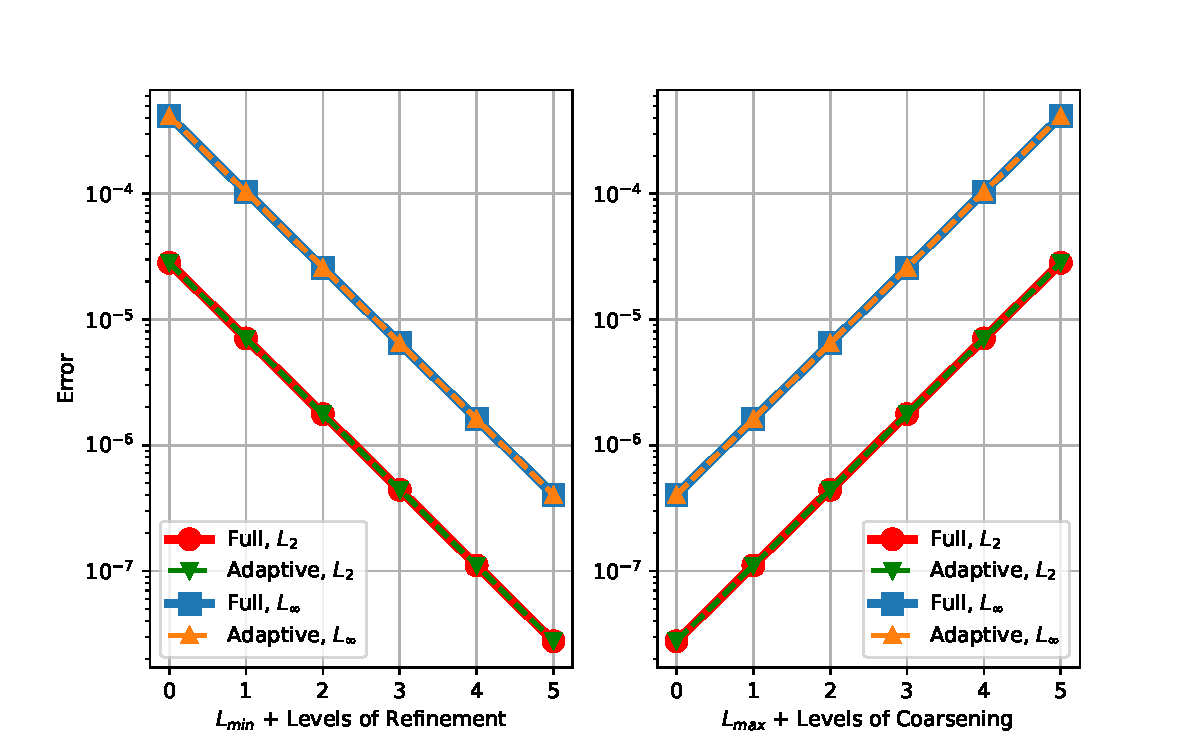
\includegraphics[width=\textwidth, clip=true, trim={40 0 40 40}]{figures/full-vs-adaptive-convergence-no-title.pdf}
    \caption{[TODO]}
    \label{fig:full-vs-adaptive-convergence}
\end{figure}

\subsection{Random Refinement}

\begin{figure}
    \centering
    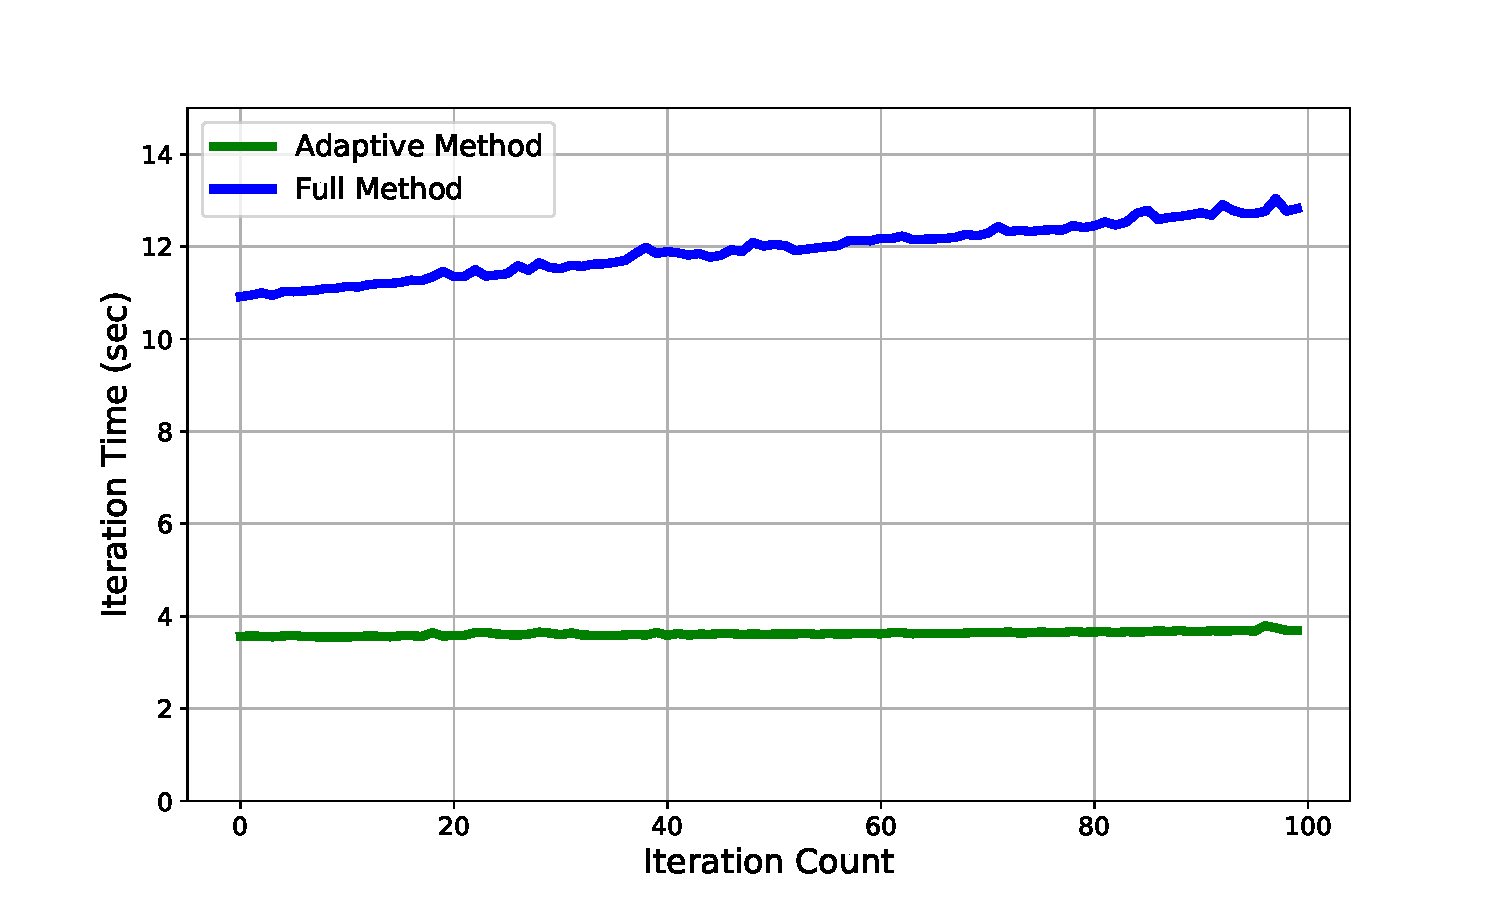
\includegraphics[width=\textwidth, clip=true, trim={40 0 40 40}]{figures/full-vs-adaptive-time-comparison-no-title.pdf}
    \caption{[TODO]}
    \label{fig:full-vs-adaptive-time-comparison}
\end{figure}
\section{Conclusion}

The work presented in this paper demonstrates a successful implementation of the quadtree-adaptive Hierarchical Poincaré-Steklov (HPS) method in parallel. The integration of the \pforest\ library, known for its efficiency and scalability, with the communication patterns of the quadtree-adaptive HPS method, shows promise for an effective solver for elliptic PDEs. As distributed memory architectures are increasingly more common in commodity clusters, an MPI implementation is essential for future scalability.

Running strong and weak scaling analysis on Polaris, one of the world's top 50 fastest supercomputers, provides insights into potential and necessary improvements for further optimizations. The current bottleneck is the communication required for the family callbacks during family traversals of the path-indexed quadtree. Potential optimizations include reducing redundant calculations through more efficient matrix partitioning and investigating non-blocking communication to better overlap compute and communication. These insights are currently being investigated and integrated into EllipticForest \citep{chipman2024ellipticforest}.

\chapter{A Parallel Implementation of the Quadtree-Adaptive HPS Method}
\label{chap:parallel}
\section{Introduction}
\label{sec:intro}

The \gls{qahps} method is a direct method for solving elliptic \gls{pdes} on a hierarchy of adaptively refined finite volume meshes. It builds upon the \gls{hps} methods first presented by \citet{gillman2014direct}, including \gls{amr} considerations found in \citep{babb2018accelerated,geldermans2019adaptive}. The primary contribution of the \gls{qahps} method is the derivation and implementation of the \gls{hps} method for use with a quadtree-style mesh with embedded finite volume meshes. In this chapter, we will derive the \gls{qahps} method, detail the implementation for use with \pforest \citep{burstedde2011p4est,burstedde2020parallel}, and provide a detailed convergence and error analysis for elliptic \gls{pdes}.
\section{The Parallel Algorithm}
\section{Parallel Results and Discussion}
\label{sec:parallel-results-and-discussion}

We demonstrate the strong and weak scaling of the current implementation. For each of the strong and weak scaling runs, we time the leaf and family callback stages for the build, upwards, and solve stages of the HPS method. This provides insight into the scalability of the leaf traversals as well as the family traversals for each stage.

For both strong and weak scaling analysis, we ran on the petascale machine Polaris at Argonne National Laboratory. Polaris is a 560 node machine, with each node consisting of one 2.8GHz AMD EPYC Milan 7543P 32 core CPU with 512 GB of DDR4 RAM.

\subsection{Strong Scaling}

Strong scaling analysis is done by solving a relatively large problem while increasing the number of compute units used to solve the problem. As one increases the parallelism, the compute per compute unit decreases at a rate equal to that at which the number of compute units is increasing. Ideal strong scaling should result in the time to solution decreasing at the same rate that the number of compute units is increasing.

Using the method of manufactured solutions, we generate a Poisson problem based on the exact solution
\begin{align}
    u_{\text{exact}}(x, y) = \sin(x) + \sin(y).
\end{align}
The resulting Poisson equation is thus
\begin{align}
    \nabla^2 u(x,y) = f(x,y) = -u_{\text{exact}}(x, y),
\end{align}
where the boundary conditions are provided by the exact solution. The leaf-indexed and path-indexed quadtrees that represent the underlying mesh are generated by recursively refining the root-level patch according to a refinement criteria of $|f(x,y)| > 1.2$. We used 8 levels of refinement, and patch sizes of $M = [8, 16, 32, 64]$. This results in solving the Poisson equation with an effective resolution of up to $8192 \times 8192$.

{\bf Results and Discussion}
The results of running on Polaris can be found in \reffig{fig:strong_scaling_plots}. For each patch size $M$ (indicated by the colors in \reffig{fig:strong_scaling_plots}), we increase the number of MPI ranks used to solve the problem. We show scaling on up to $N_R = 128$ MPI ranks.

\begin{figure}
    \centering
    \begin{tabular}{c}
        \begin{subfigure}[t]{0.95\textwidth}
            \centering
            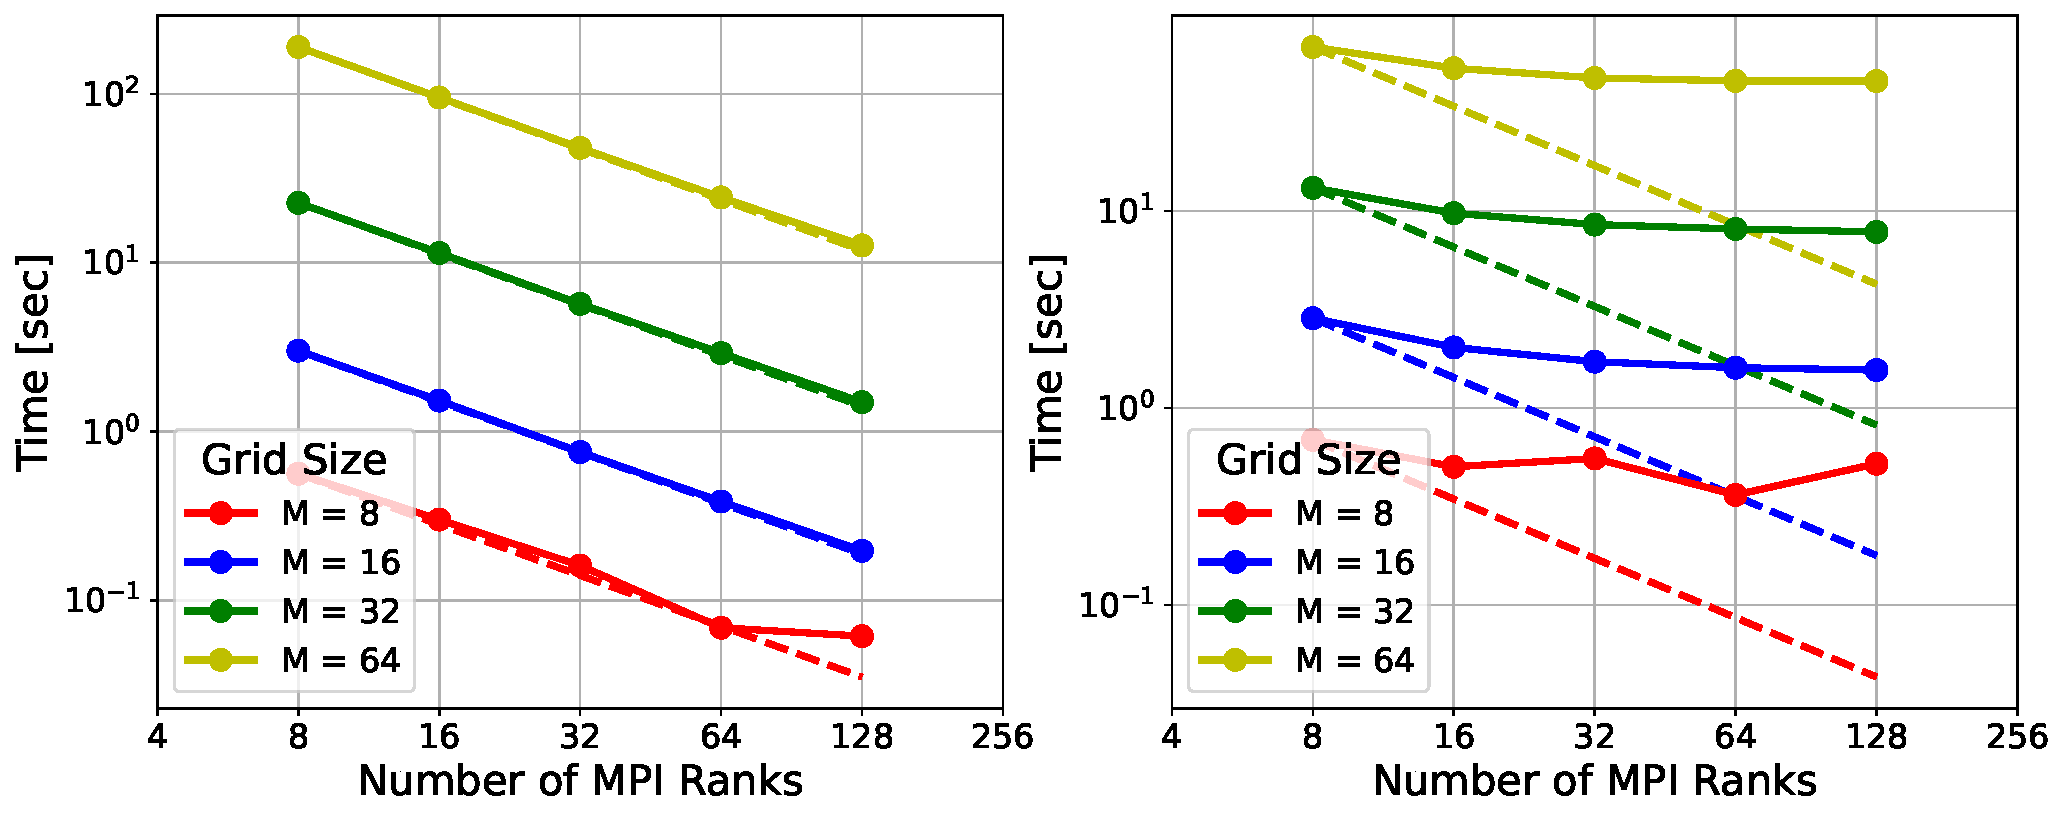
\includegraphics[width=\textwidth]{figures/build-strong-scaling-timing-no-title.pdf}
            \caption{The build stage strong scaling.}
            \label{subfig:strong_build}
        \end{subfigure}
        \\
        \begin{subfigure}[t]{0.95\textwidth}
            \centering
            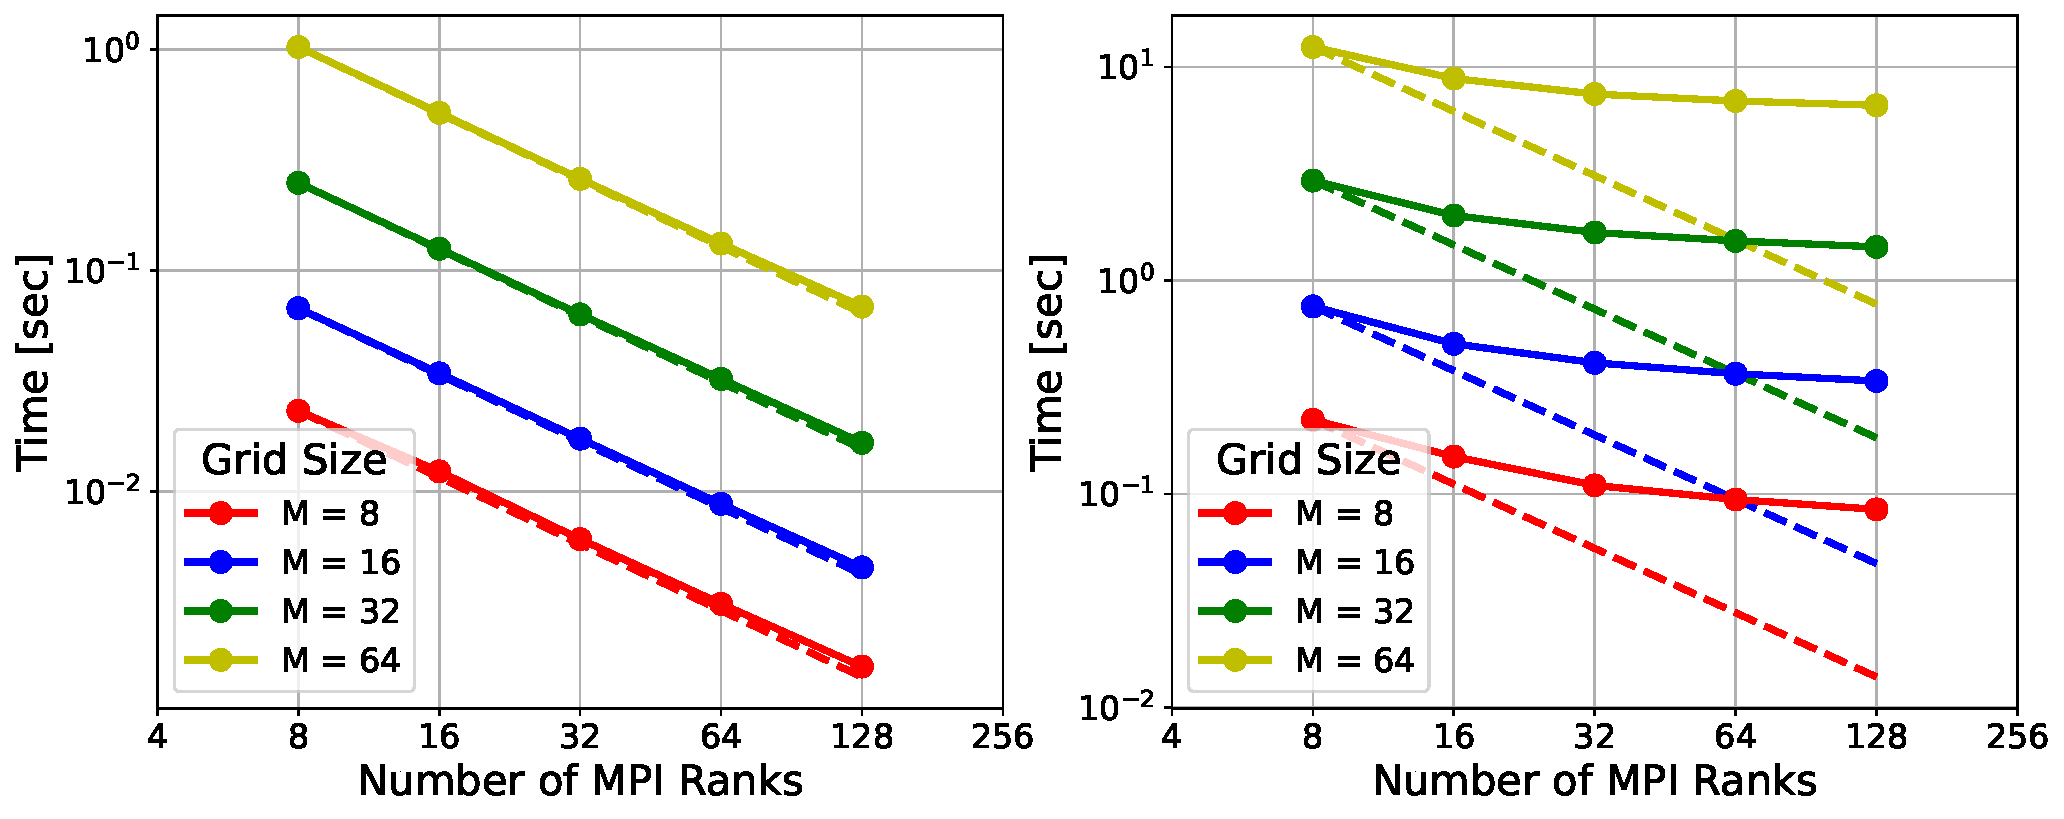
\includegraphics[width=\textwidth]{figures/upwards-strong-scaling-timing-no-title.pdf}
            \caption{The upwards stage strong scaling.}
            \label{subfig:strong_upwards}    
        \end{subfigure}
        \\
        \begin{subfigure}[t]{0.95\textwidth}
            \centering
            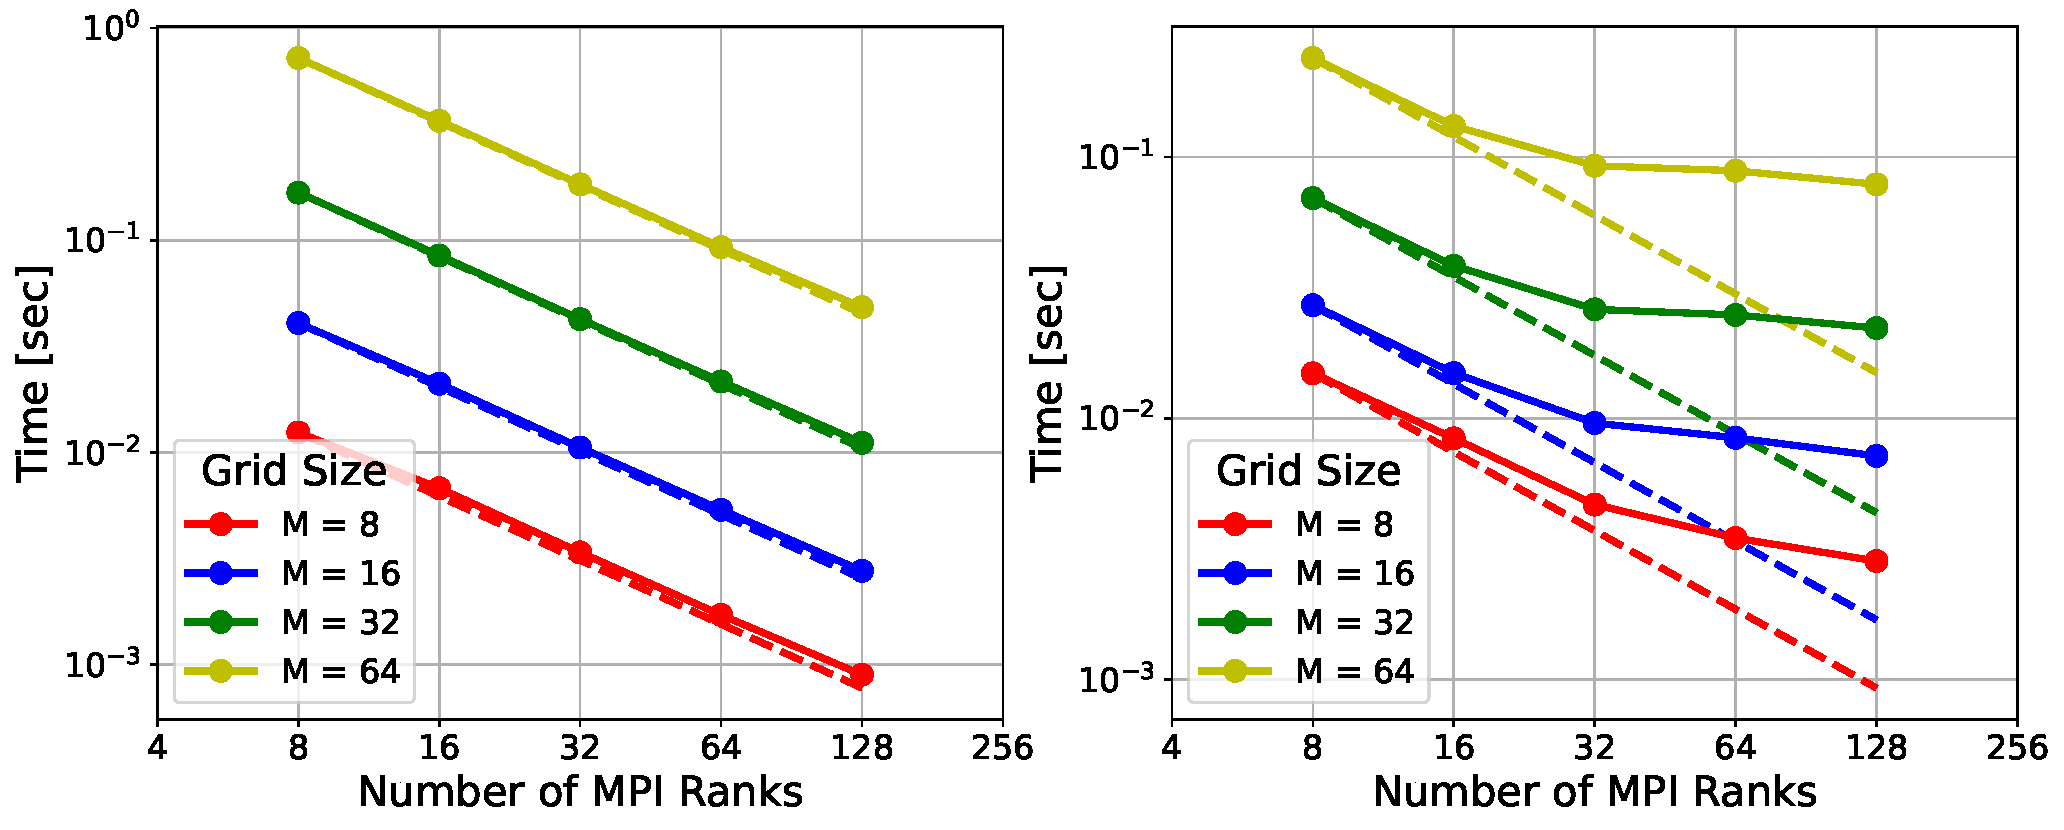
\includegraphics[width=\textwidth]{figures/solve-strong-scaling-timing-no-title.pdf}
            \caption{The solve stage strong scaling.}
            \label{subfig:strong_solve}
        \end{subfigure}
        \\
    \end{tabular}
    \caption{The strong scaling plots for the (a) build stage, (b) upwards stage, and (c) solve stage. For each, the left plot shows the scaling for the leaf callback and the right plot shows the scaling for the family callback. The solid line indicates actual timing and the dashed line indicates ideal strong scaling.}
    \label{fig:strong_scaling_plots}
\end{figure}

\reffig{fig:strong_scaling_plots} shows that the leaf callback functions for all three stages scale nearly perfectly. This is to be expected as there is no communication at this stage; each partition builds up the factorization or solves the elliptic problem independently. The family callbacks for all three stages have less than optimal scaling. In each stage, the family callback includes communicating data across families. Sibling nodes at intermediate levels (i.e., non-leaf nodes) are often owned by multiple ranks. The communication among ranks at the upper levels involves potentially global communication, including broadcast operations. This amount of communication is what leads to poor strong scaling at medium to larger runs; the amount of communication grows much faster than the compute time.

Comparing the strong scaling between the three different stages shows that the solve stage scales better than the build and the upwards stages. The size of the data involved in the communication in the solve stage is smaller than that in the factorization stages.

% \begin{figure}
%     \centering
%     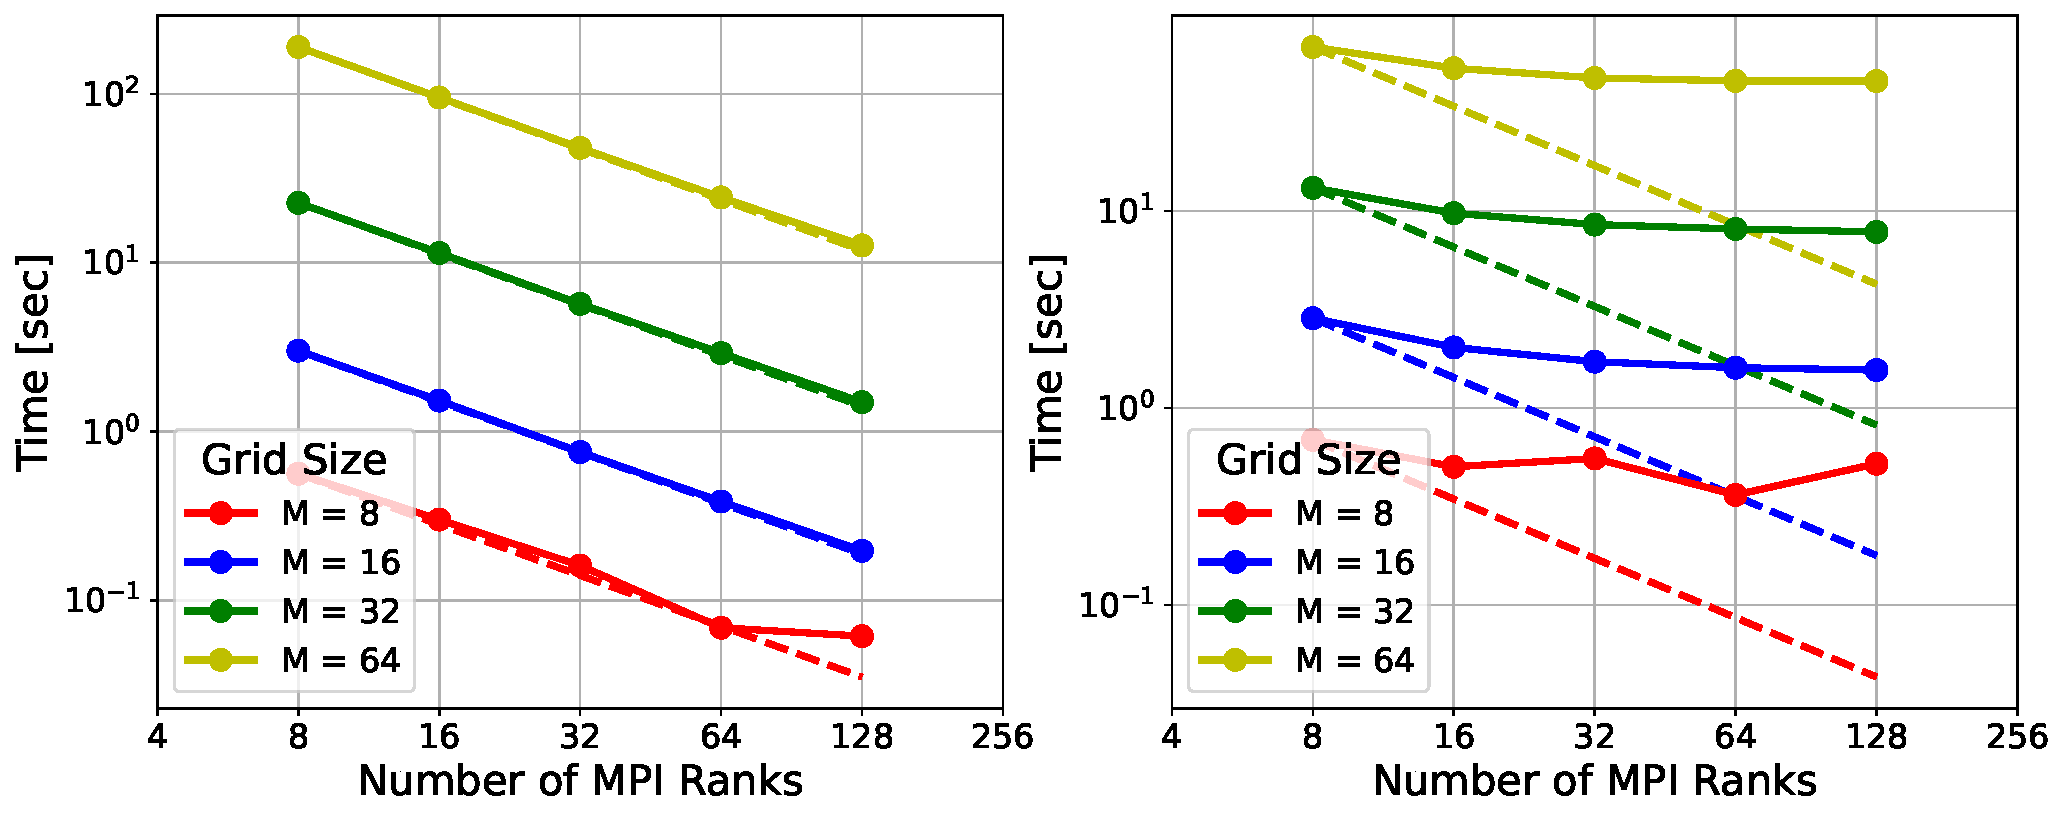
\includegraphics[width=\textwidth]{figures/build-strong-scaling-timing-no-title.pdf}
%     \caption{The strong scaling for the build stage. The left plot shows the scaling for the leaf callback and the right plot shows the scaling for the family callback. The solid line indicates actual timing and the dashed line indicates ideal strong scaling.}
%     \label{fig:strong_build}
% \end{figure}

% \begin{figure}
%     \centering
%     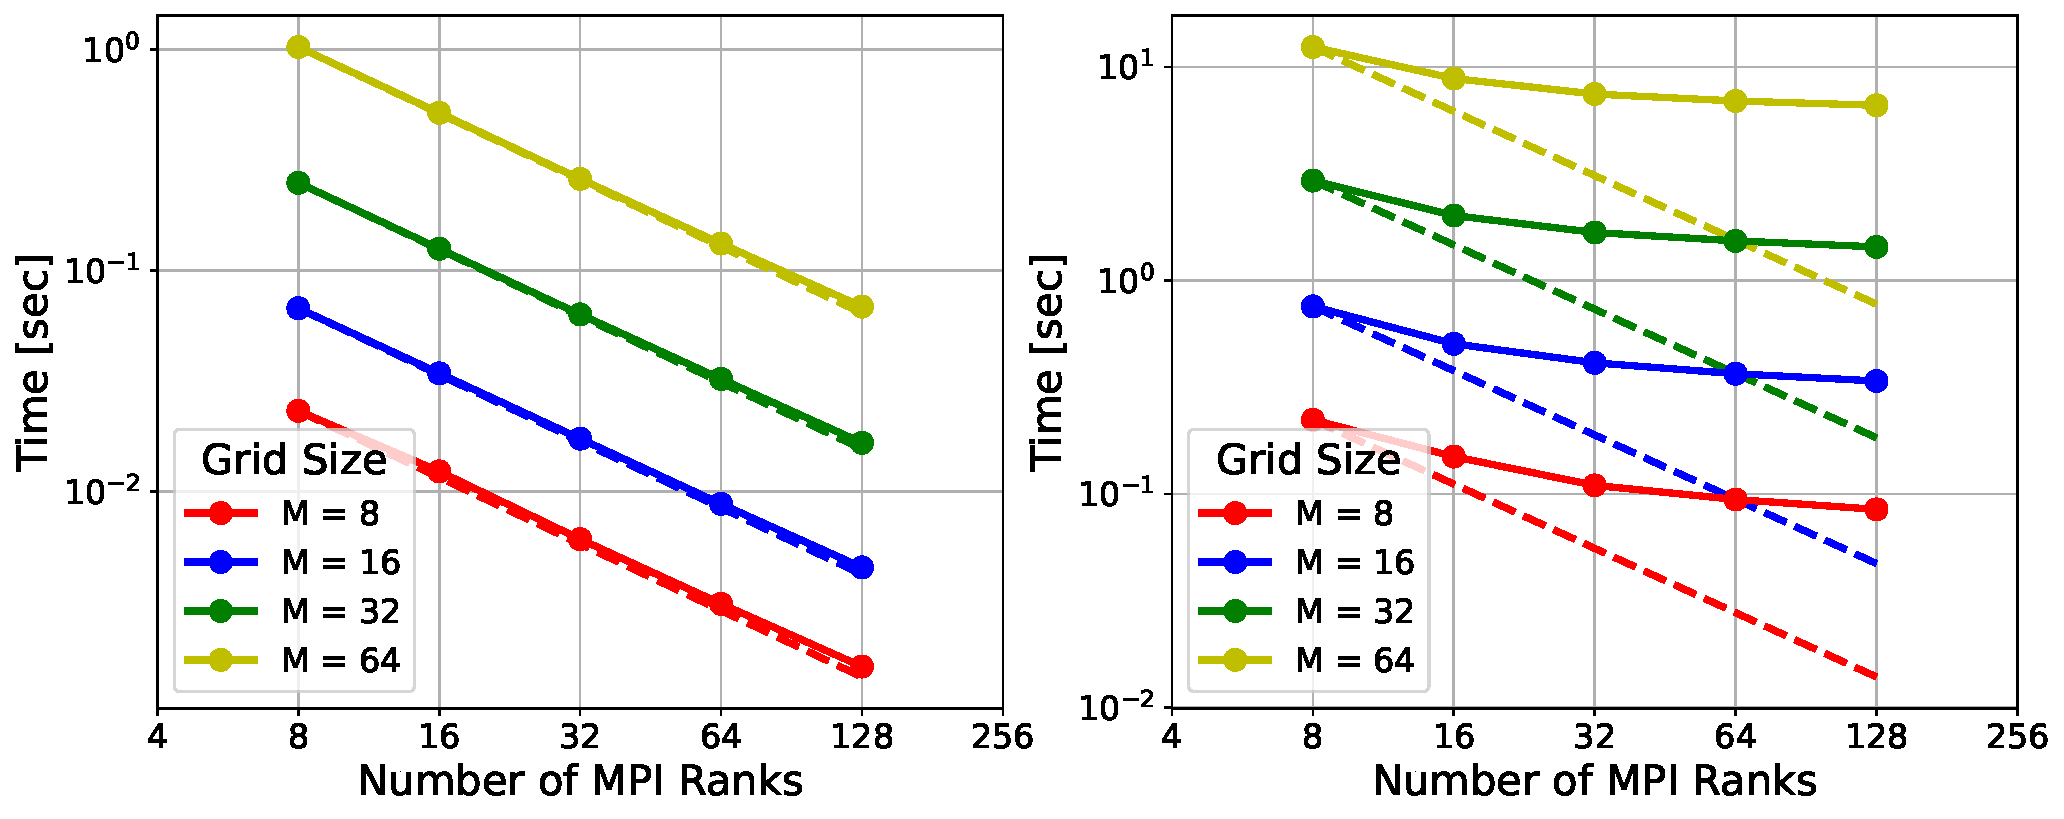
\includegraphics[width=\textwidth]{figures/upwards-strong-scaling-timing-no-title.pdf}
%     \caption{The strong scaling for the upwards stage. The left plot shows the scaling for the leaf callback and the right plot shows the scaling for the family callback. The solid line indicates actual timing and the dashed line indicates ideal strong scaling.}
%     \label{fig:strong_upwards}
% \end{figure}

% \begin{figure}
%     \centering
%     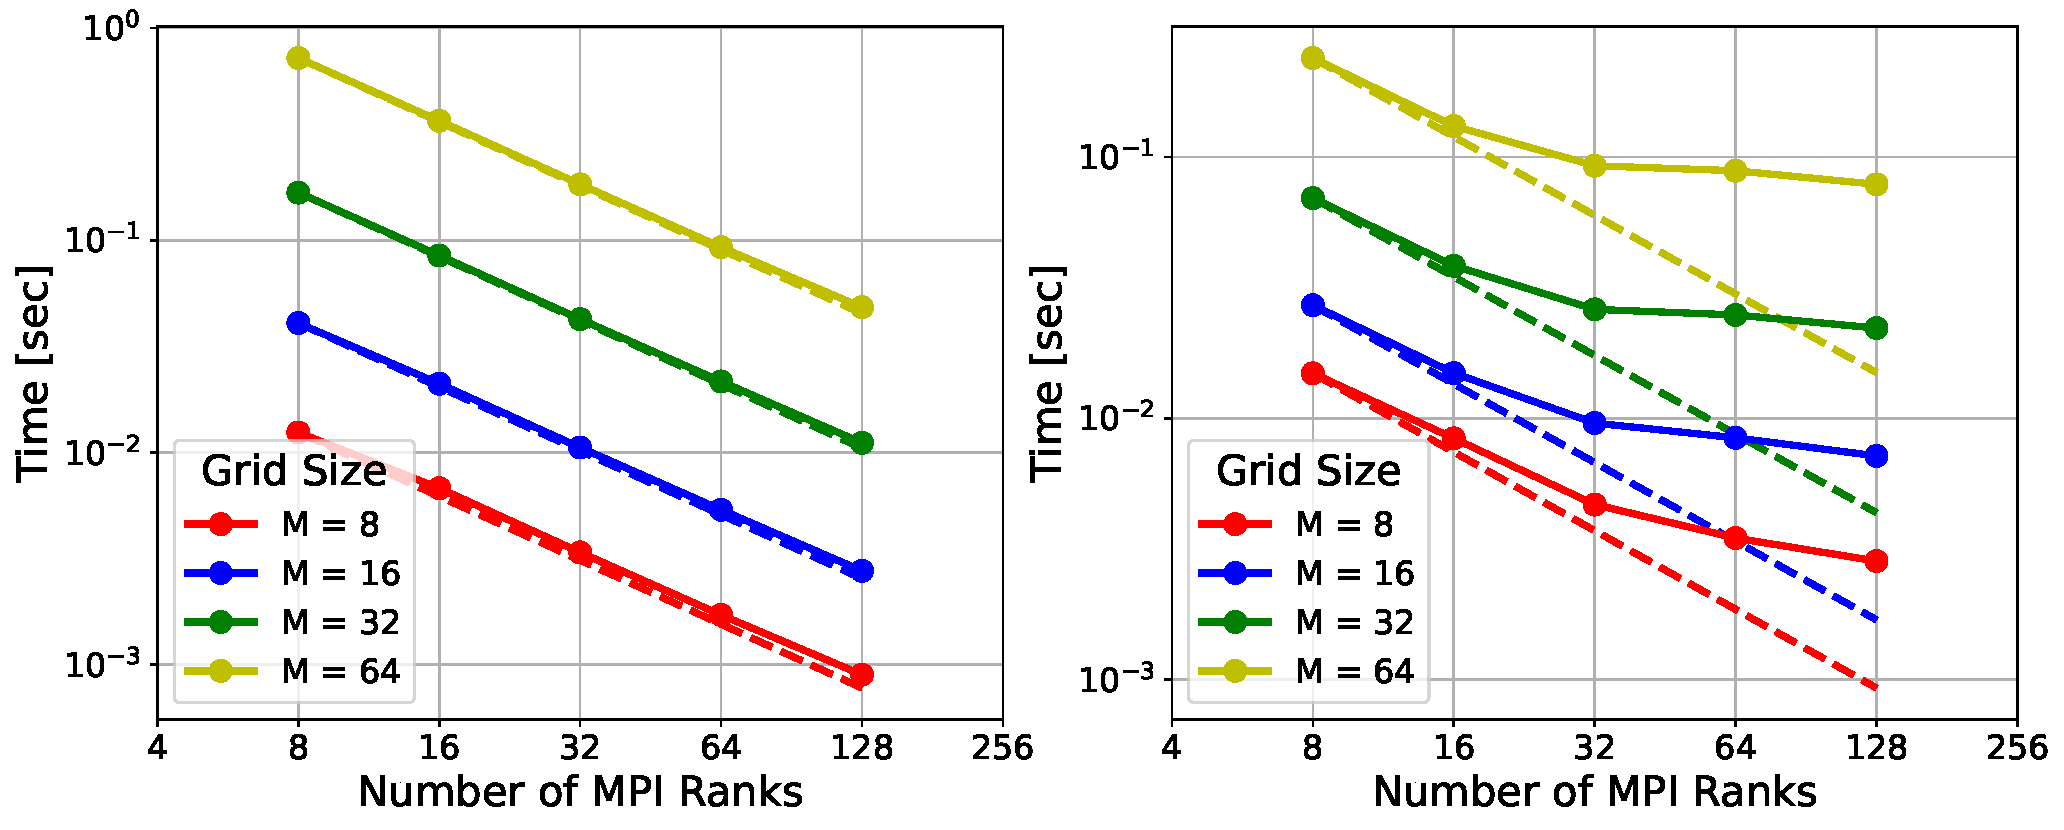
\includegraphics[width=\textwidth]{figures/solve-strong-scaling-timing-no-title.pdf}
%     \caption{The strong scaling for the solve stage. The left plot shows the scaling for the leaf callback and the right plot shows the scaling for the family callback. The solid line indicates actual timing and the dashed line indicates ideal strong scaling.}
%     \label{fig:strong_solve}
% \end{figure}

\subsection{Weak Scaling}
\label{sub:weak-scaling}

Weak scaling analysis is done by solving a problem while increasing both the size of the problem and the number of compute units. The compute time per compute unit stays constant in a weak scaling analysis and time to solution should stay constant as one increases the parallelism.

We solve the polar star Poisson problem with one polar star per compute unit (see \refsec{sub:example-two}). To keep the number of degrees of freedom constant per MPI rank, we solve on a square domain with a single polar star at the center. With each increase in the number of MPI ranks, we extend the domain to include more polar stars, each at the center of their own partition.

For this study, we refine around the edges of the polar stars. The refinement criteria was $|f(x,y)| > 1$, with 7 levels of refinement. Each polar star was a 4-pointed polar star with $r_0 = 0.3$, $r_1 = 0.4$, and $\epsilon = 0.015625$. We solve with patch sizes $M = [16, 32, 64]$, resulting in the degrees of freedom per MPI rank to be $[4096, 16384, 65536]$, respectively. An example of this setup can be found in \reffig{fig:polar-star-plots}, which shows the repeated solution and partitioning for $N_R = 4$ arranged in a $2 \times 2$ grid of processes.

\begin{figure}
    \centering
    \begin{tabular}{c c}
        \begin{subfigure}[t]{0.45\textwidth}
            \centering
            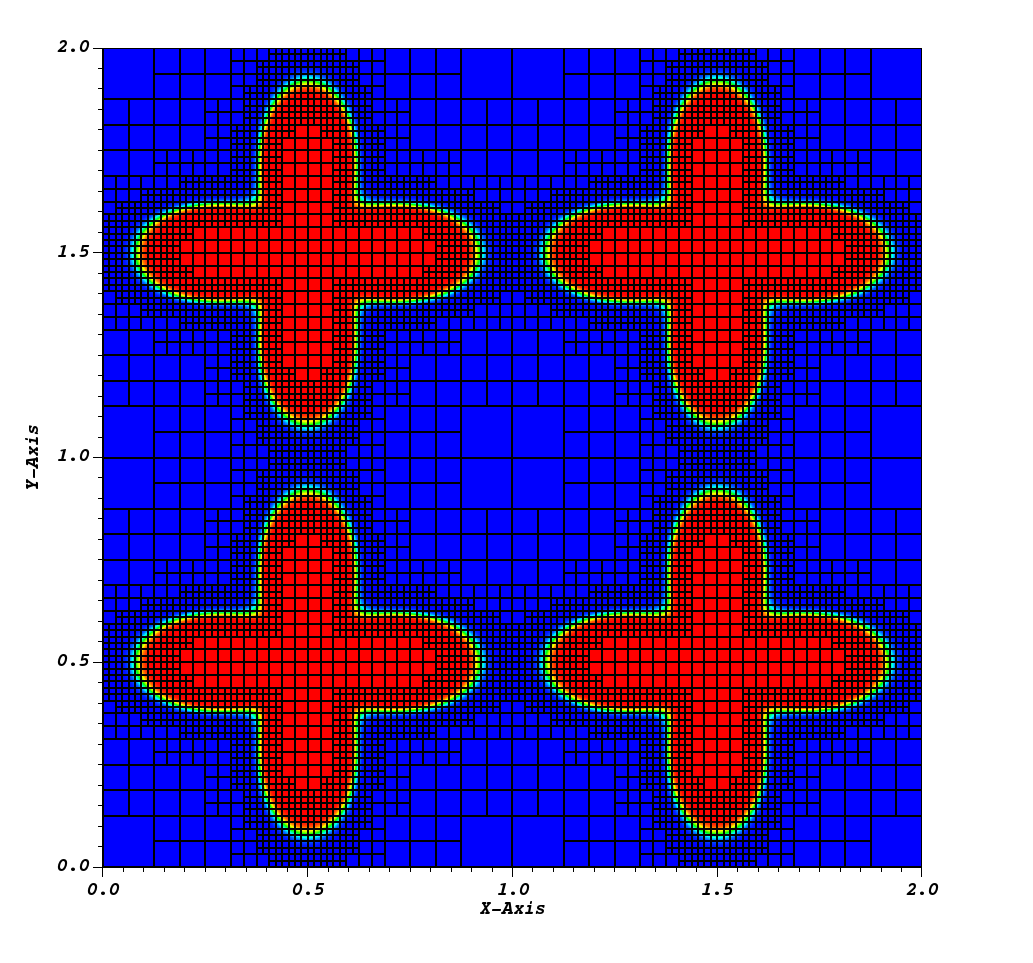
\includegraphics[width=\textwidth, clip=True, trim={0 0 0 0}]{figures/weak-scaling-stars.png}
            \caption{The plotted solution.}
            \label{subfig:polar-star-solution}
        \end{subfigure}
        &
        \begin{subfigure}[t]{0.45\textwidth}
            \centering
            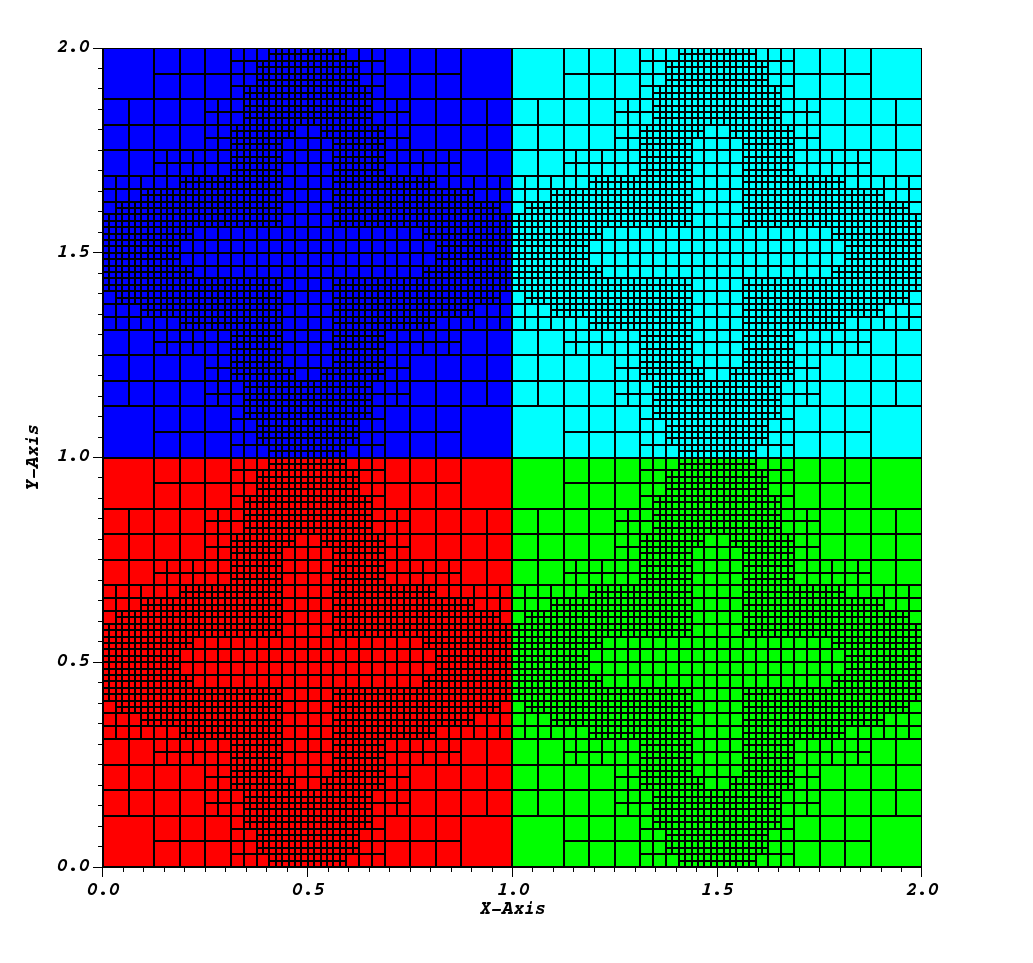
\includegraphics[width=\textwidth, clip=True, trim={0 0 0 0}]{figures/weak-scaling-partitions.png}
            \caption{The MPI partitions.}
            \label{subfig:polar-star-partitions}
        \end{subfigure}
    \end{tabular}
    \caption{Plots of the polar star Poisson problem used in the weak scaling study found in \refsec{sub:weak-scaling}. The polar star is generated from the RHS of the Poisson equation and is repeated for each MPI rank used to solve the problem. This shows four polar stars arranged in a $2 \times 2$ grid for solving with $N_R = 4$. Each outlined grid contains a $16 \times 16$ finite volume mesh.}
    \label{fig:polar-star-plots}
\end{figure}

{\bf Results and Discussion}
\reffig{fig:weak_scaling_plots} contains the results of the weak scaling runs. We plot the weak scaling efficiency, which is computed as
\begin{align}
    E_{\text{weak}} = \frac{t_{1}}{t_{N_R}} \times 100 \%,
\end{align}
where $t_{1}$ is the time spent in that stage on a single MPI rank. The colors indicate the different patch sizes, and the leaf and family callbacks are shown for all three stages.

Similarly to the strong scaling, the leaf callbacks scale better than the family callbacks. The build stage and solve stage leaf callbacks maintain nearly perfect weak scaling efficiency. The upwards stage scales similarly to the scaling of the family callbacks, which is unexpected. The family callbacks demonstrate similar scaling drop off as in the strong scaling. Again, this is likely due to the increased communication, along with the redundant calculations exhibited in this implementation.

\begin{figure}
    \centering
    \begin{tabular}{c}
        \begin{subfigure}[t]{0.95\textwidth}
            \centering
            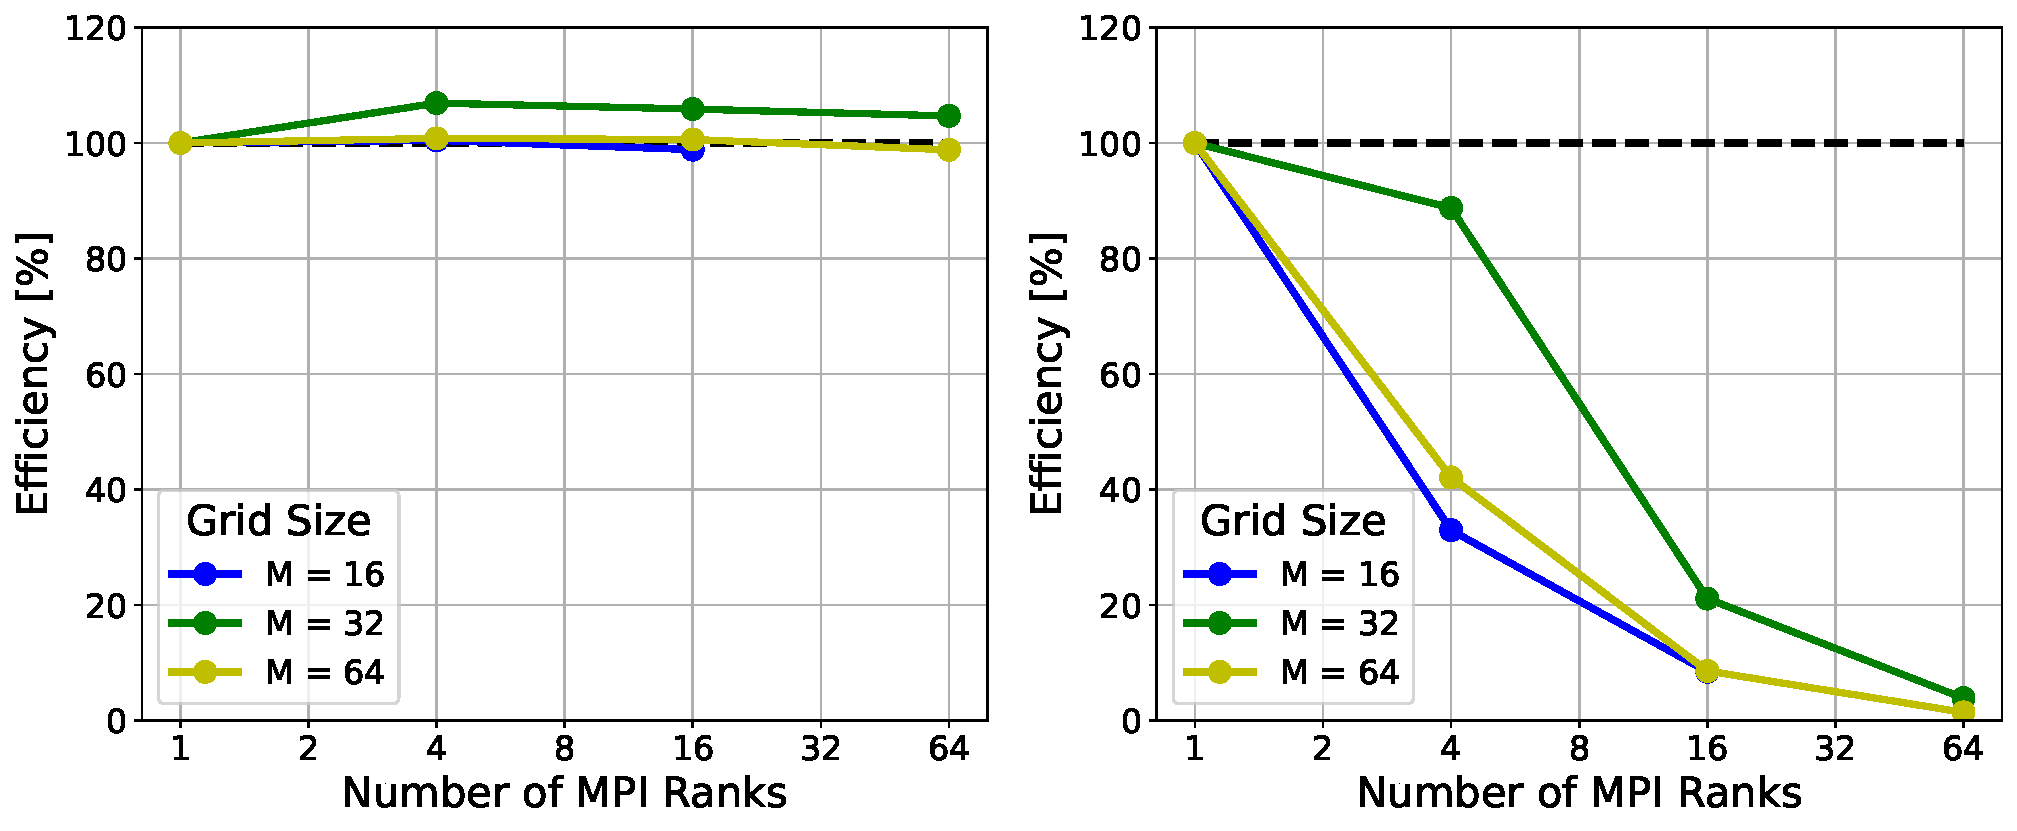
\includegraphics[width=\textwidth]{figures/build-weak-scaling-timing-no-title.pdf}
            \caption{The build stage weak scaling.}
            \label{subfig:weak_build}
        \end{subfigure}
        \\
        \begin{subfigure}[t]{0.95\textwidth}
            \centering
            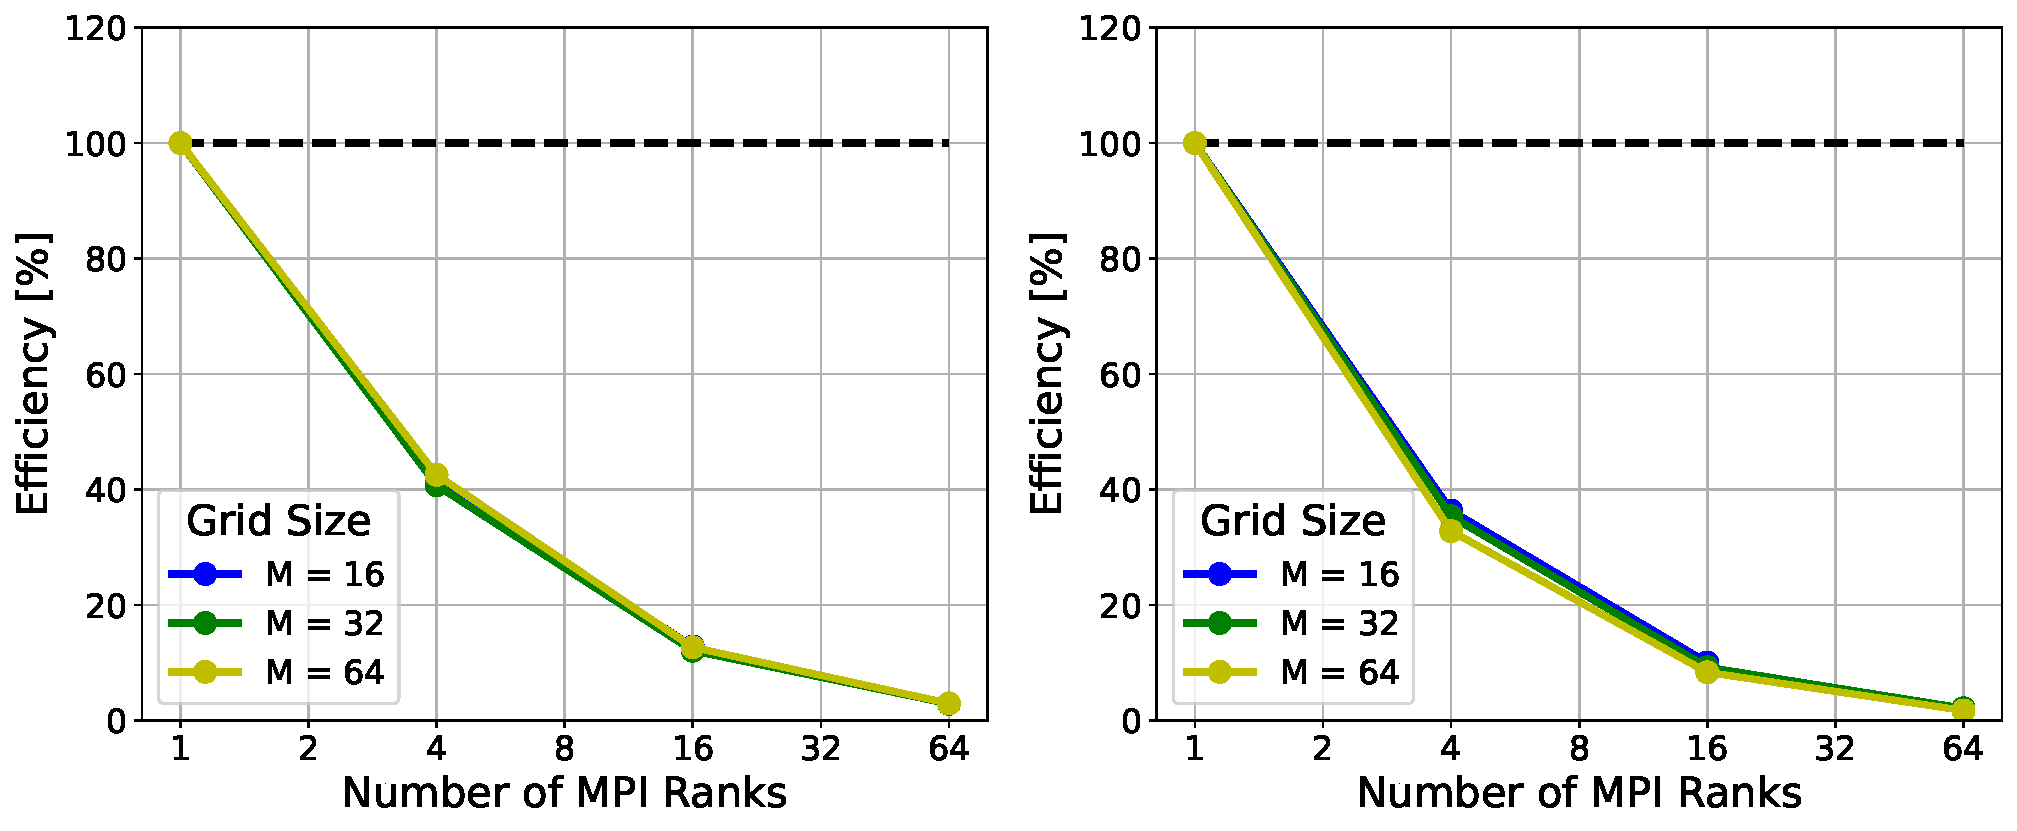
\includegraphics[width=\textwidth]{figures/upwards-weak-scaling-timing-no-title.pdf}
            \caption{The upwards stage weak scaling.}
            \label{subfig:weak_upwards}    
        \end{subfigure}
        \\
        \begin{subfigure}[t]{0.95\textwidth}
            \centering
            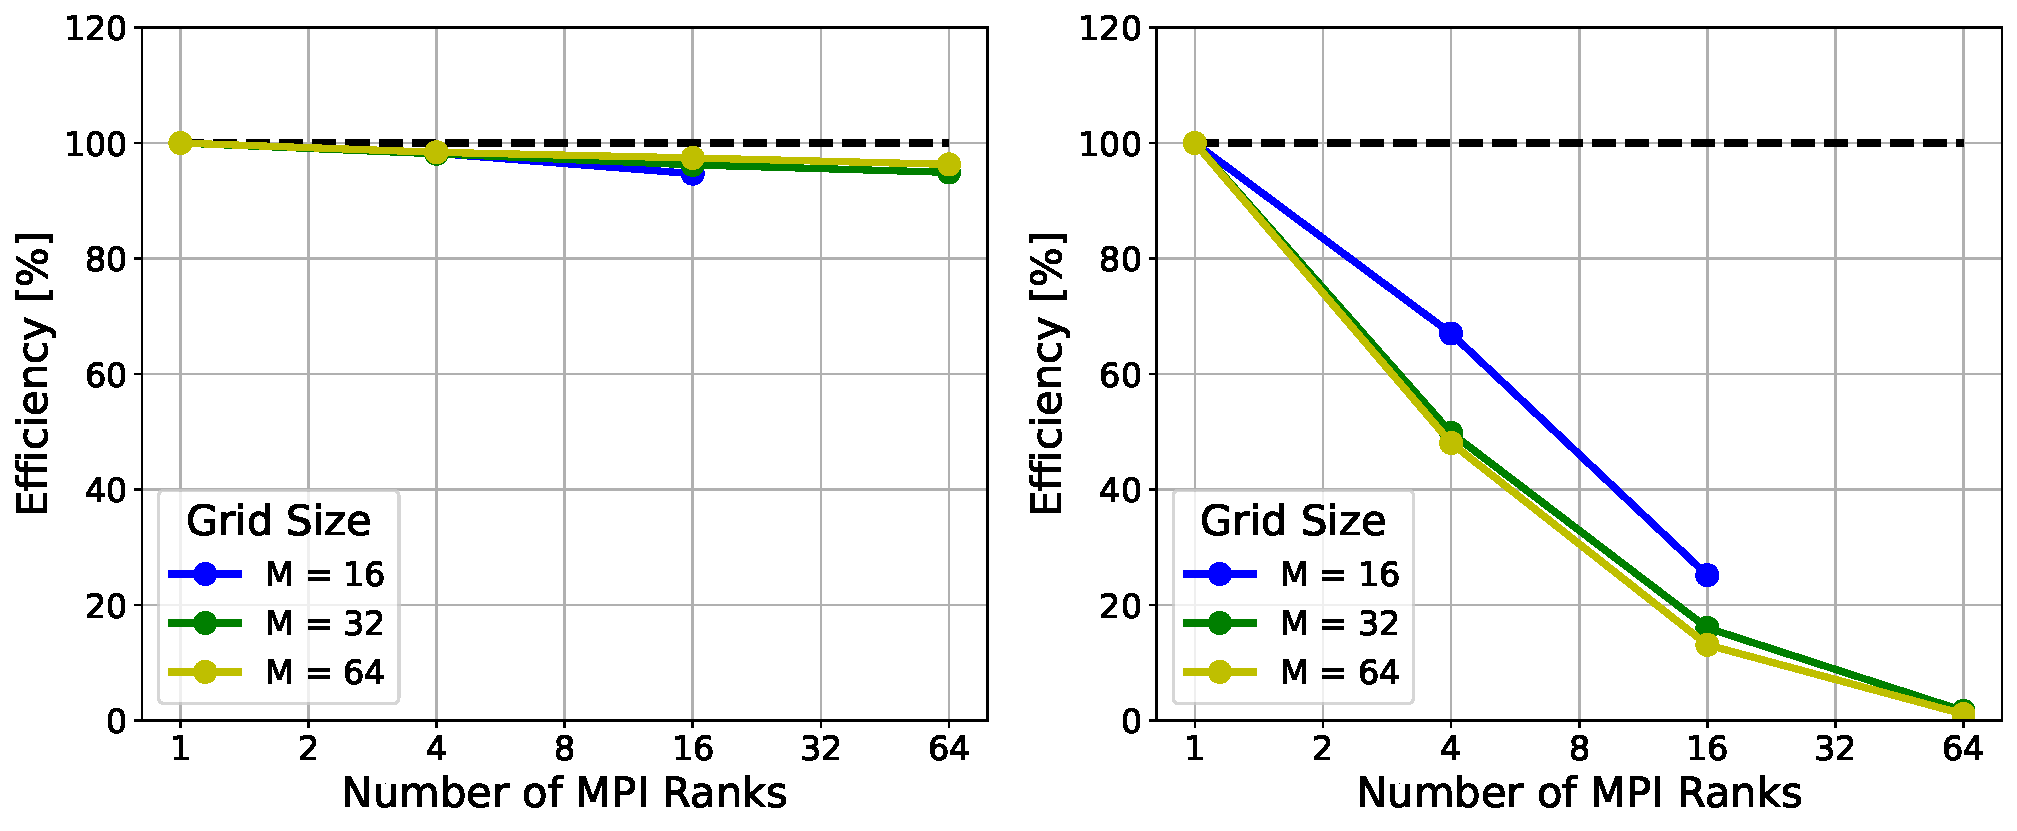
\includegraphics[width=\textwidth]{figures/solve-weak-scaling-timing-no-title.pdf}
            \caption{The solve stage weak scaling.}
            \label{subfig:weak_solve}
        \end{subfigure}
        \\
    \end{tabular}
    \caption{The weak scaling plots for the (a) build stage, (b) upwards stage, and (c) solve stage. For each, the left plot shows the scaling for the leaf callback and the right plot shows the scaling for the family callback. The solid line indicates actual efficiency and the dashed line indicates ideal weak scaling.}
    \label{fig:weak_scaling_plots}
\end{figure}

% \begin{figure}
%     \centering
%     \includegraphics[width=\textwidth]{figures/build-weak-scaling-timing-no-title.pdf}
%     \caption{The weak scaling for the build stage. The left plot shows the scaling for the leaf callback and the right plot shows the scaling for the family callback. The solid line indicates actual timing and the dashed line indicates ideal weak scaling.}
%     \label{fig:weak_strong_build}
% \end{figure}

% \begin{figure}
%     \centering
%     \includegraphics[width=\textwidth]{figures/upwards-weak-scaling-timing-no-title.pdf}
%     \caption{The weak scaling for the upwards stage. The left plot shows the scaling for the leaf callback and the right plot shows the scaling for the family callback. The solid line indicates actual timing and the dashed line indicates ideal weak scaling.}
%     \label{fig:weak_strong_upwards}
% \end{figure}

% \begin{figure}
%     \centering
%     \includegraphics[width=\textwidth]{figures/solve-weak-scaling-timing-no-title.pdf}
%     \caption{The weak scaling for the solve stage. The left plot shows the scaling for the leaf callback and the right plot shows the scaling for the family callback. The solid line indicates actual timing and the dashed line indicates ideal weak scaling.}
%     \label{fig:weak_strong_solve}
% \end{figure}
\section{Conclusion}

The work presented in this paper demonstrates a successful implementation of the quadtree-adaptive Hierarchical Poincaré-Steklov (HPS) method in parallel. The integration of the \pforest\ library, known for its efficiency and scalability, with the communication patterns of the quadtree-adaptive HPS method, shows promise for an effective solver for elliptic PDEs. As distributed memory architectures are increasingly more common in commodity clusters, an MPI implementation is essential for future scalability.

Running strong and weak scaling analysis on Polaris, one of the world's top 50 fastest supercomputers, provides insights into potential and necessary improvements for further optimizations. The current bottleneck is the communication required for the family callbacks during family traversals of the path-indexed quadtree. Potential optimizations include reducing redundant calculations through more efficient matrix partitioning and investigating non-blocking communication to better overlap compute and communication. These insights are currently being investigated and integrated into EllipticForest \citep{chipman2024ellipticforest}.

\chapter{Software and Code Comparisons}
\label{chap:software-and-code}
\section{Introduction}

Elliptic \gls{pdes} describe phenomena in the areas of physics, biology, chemistry, engineering, and others. In physics, potential fields such as gravitational fields and electromagnetic fields are modeled with elliptic PDEs (the Laplace and Poisson equations). In biology and chemistry, reaction-diffusion systems can be characterized using time-dependent elliptic operators. Engineering examples include heat and mass diffusion, as well as pressure calculations for viscous fluid systems. Scientists and engineers modeling these various phenomena must solve the associated elliptic equations using analytical and/or numerical methods.

Numerical methods for elliptic PDEs is a well-documented area of research and development. Classical methods include finite difference, finite volume, and finite element methods. More modern approaches include higher order versions of classical methods, spectral methods, and meshless approaches like particle based methods or radial basis function techniques. Many discretization approaches results in a system of linear equations that must be solved efficiently and rapidly. Solution methods are categorized into direct and iterative methods, each with their own advantages and disadvantages. Taking advantage of the structure of the linear systems leads to significant increases in memory and compute performance.

Modern compute resources are as diverse as they are extensive. From high-powered laptops, to desktop workstations, to clusters and supercomputers, there is no lack of available platforms for scientific modeling. With diverse hardware and software stacks, the numerical methods developed to solve the aforementioned linear systems should be versatile and adaptable, capable of leveraging the specific characteristics and strengths of each type of hardware. Optimizations such as vectorization, parallelization, and memory access patterns must be carefully considered and implemented to maximize performance across different platforms.

Adaptive mesh refinement (AMR) is a mesh technique used to increase the memory and compute efficiency of numerical solvers for PDEs. AMR techniques collocate more refined meshes around targeted regions of interest, and coarser meshes elsewhere. Localized regions of error, large gradients, boundaries, and material interfaces are examples of regions where higher resolution is beneficial. Adaptive meshes can significantly improve the performance of numerical solvers, at the cost of more complicated implementations. Additional considerations must be accounted for, such as how to handle coarse-fine interfaces, load balancing for parallel algorithms, and more complicated data structures. In the context of elliptic PDEs, AMR further complicates linear solvers; iterative preconditioners must be more sophisticated and expensive matrix factorizations must be recomputed when the mesh is adapted. Although AMR introduces complexities, the benefits often outweigh the cost as the use of AMR enables the modeling of complex phenomena when more traditional uniform solvers are too computationally expensive.

This dissertation will detail the development of a direct solver for elliptic PDEs that can be applied to adaptive meshes efficiently and for parallel computer architectures. The method is called the \gls{qahps} method. The primary feature of this method is that the factorization is represented as a set of solution operators that can be locally adapted. The method is an adaptive extension of the \gls{hps} method \citep{gillman2014direct} and targets a tree-based AMR approach as implemented in the \pforest software library \citep{burstedde2011p4est}. Building the factorization set can be done with $\mathcal{O}(N^{3/2})$ complexity, with $\mathcal{O}(N)$ complexity for subsequent solves. Parallelization is handled for distributed memory computer architectures through the \gls{mpi}. It will be shown that the method motivated and developed herein is competitive with other codes and solvers, including iterative solvers for elliptic PDEs.
\section{Software for Case Studies}

\subsection{EllipticForest}
\label{sub:elliptic-forest}

EllipticForest contains a user extendable and coupling-ready implementation of the \gls{qahps} method. It uses modern object-oriented software features for users to extend patch classes for different discretizations and patch solvers. All of the features of the algorithms outlined in this dissertation are able to be used, including optimized solvers for constant coefficient problems, parallelism, and adaptivity.

\subsection{ForestClaw and ThunderEgg}
\label{sub:thunder-egg}

ThunderEgg \citep{aiton2022thunderegg} is a repository that contains multigrid solvers and preconditioners for elliptic \gls{pdes} for \gls{amr}. Similarly to EllipticForest, it is built on top of \pforest \citep{burstedde2011p4est,burstedde2020parallel} for efficient mesh management. It supports parallelism through MPI \citep{mpi40}.

ThunderEgg is coupled into the ForestClaw library. ForestClaw \citep{calhoun2017forestclaw} is a software library containing parallel, multi-block adaptive finite volume solvers for \gls{pdes}. ForestClaw also extends \pforest \citep{burstedde2011p4est,burstedde2020parallel} with multiple \gls{pdes} solvers. These cases are solved with the ForestClaw interface to ThunderEgg.

\subsection{PETSc}
\label{sub:petsc}

The Portable, Extensible Toolkit for Scientific Computing (PETSc) is a software library for scalable scientific applications. It supports MPI \citep{mpi40} for distributed memory parallelism and GPUs through multiple vendor backends (CUDA, HIP, Kokkos, OpenCL). The design of PETSc allows for users to implement a discretization to solve a \gls{pde} (for example, a five point stencil finite difference discretization), and then use any number of compatible solvers and preconditioners. The matrix type (sparse, dense, CPU, GPU), the preconditioner type, the solver type, and many other options can be changed at runtime.

The solvers for the elliptic cases in this chapter are extended from the examples in the book by \cite{bueler2020petsc}.
\section{Case Studies}
\label{sec:case-studies}

Here we examine three case studies involving elliptic \gls{pdes}. For all iterative methods, the relative tolerance is set to $\tau_{\text{rel}} = 1 \times 10^{-12}$ and the maximum number of iterations allowed is $N_{\textsc{max}} = 10000$. For all cases, the effective resolution, which is the resolution of the domain at the finest level if the mesh is adaptive, will vary from $R_{\text{eff}} = [128, 256, 512, 1024, 2048]$. All runs were done in parallel on a 2021 MacBook Pro (M1 Pro CPU with 8 cores, 32GB RAM).

\subsection{Case 1: The Poisson Equation}
\label{sub:case01}

The first case study solves
\begin{align}
    \nabla^2 u(x,y) = -2(y^2 - y^4 + x^4(6y^2 - 1) + x^2 (1 - 12y^2 + 6^4))
\end{align}
for $(x,y) \in \Omega = [-1,1]^2$, which has the exact solution
\begin{align}
    u(x,y) = x^2 (1 - x^2) y^2 (y^2 - 1).
\end{align}
Dirichlet boundary conditions are supplied at the boundary using the exact solution. This problem is chosen to allow for refinement at the corners for any solver that can take advantage of adaptivity.

For adaptive solvers, the mesh is refined according to the right-hand side, which represents the curvature of the solution and is a good first attempt at \gls{amr} for elliptic \gls{pdes}. The levels range from $L_{\text{min}} = 2$ to $L_{\text{max}} = 5$ and the refinement threshold is $\epsilon_R = 0.5$.

% \begin{landscape}
    \begin{figure}
        \centering
        \includegraphics[width=1.0\textwidth, clip=true, trim={0 0 0 0}]{figures/case01-stacked-bar-plot-comparisons-no-title.pdf}
        \caption{Effective resolution vs. timing plot for case study one (\refsec{sub:case01}). The effective resolution is the number of cells per side if the mesh were refined to $L_{\text{max}}$. Each color indicates a different method/solver. Patterns indicate different stages or preconditioners. Lower is better.}
        \label{fig:case01-stacked-bar-plot}
    \end{figure}
% \end{landscape}

\begin{figure}
    \centering
    \includegraphics[width=1.0\textwidth, clip=true, trim={0 0 0 0}]{figures/case01-work-precision-plots-no-title.pdf}
    \caption{Work-precision plot for case study one (\refsec{sub:case01}). Colors indicate different methods and solvers, while markers indicate the type of preconditioner for certain iterative solvers. For work-precision plots, curves that lie in the lower-left portion of the plot are better.}
    \label{fig:case01-work-precision-plot}
\end{figure}

{\bf Discussion}
When using a five-point stencil approach to solve the Poisson equation, the resulting linear system is \gls{spd}. For the \gls{qahps} method, this means we can employ optimizations in the build stage such as operator caching (see \refrem{thm:operator-caching}) and when building the \gls{d2n} matrix (see \refsec{sub:building-leaf-level-operators}). As a constant coefficient elliptic \gls{pde}, we can use the FISHPACK patch solver which is faster than the five-point stencil patch solver. For iterative methods, we can use the \gls{cg} method which has spectral convergence. For this case study, we show results with PETSc's \gls{cg} solver as well as \gls{gmres}, each with either a block Jacobi or \gls{amg} preconditioner. Timing results for increasing resolution is found in \reffig{fig:case01-stacked-bar-plot} and a work-precision plot is found in \reffig{fig:case01-work-precision-plot}.

The stacked bar plot in \reffig{fig:case01-stacked-bar-plot} shows timing results for increasing effective resolution. It shows how each code/method compares against each other in time to solution for the Poisson equation. For the \gls{qahps} methods (uniform and adaptive), the time to solution is partitioned into the build, upwards, and solve stages.

At the lower resolutions, PETSc's iterative solvers are very fast to converge. As the effective resolution increases, the time to solution for the block Jacobi preconditioners rapidly increases, while the \gls{amg} preconditioned solvers scale better.

Comparing iterative solvers against direct solvers, uniform \gls{qahps} has a faster time to solution than uniform, block Jacobi preconditioned \gls{gmres} at $R_{\text{eff}} \ge 512$. Adaptive \gls{qahps} is faster than uniform block Jacobi preconditioned \gls{cg} at $R_{\text{eff}} \ge 512$. In all cases, PETSc's \gls{amg} preconditioned \gls{cg} and \gls{gmres} solvers have a faster time to solution than the \gls{qahps} method. However, the major advantage of \gls{qahps} is that each subsequent elliptic solve will only need to perform the upwards and solve stages (the top two sections of the EllipticForest bars). Even if the mesh is adapted, the adaptive-rebuild feature of the \gls{qahps} method will yield subsequent time to solutions on the same order of magnitude to that of the solve stage.

\reffig{fig:case01-work-precision-plot} shows a work-precision plot for each of the methods used in case one. With work-precision plots, curves that lie in the lower-left portion of the plot are desirable. This plot verifies that all methods employed for this case accurately solve the problem, and it shows that the iterative solvers converged to an accurate solution. Although PETSc's solvers are, in general, faster and more accurate, the direct solvers of EllipticForest show a more reliable convergence curve. This is a desirable feature for solvers used in a ``block-box'' implementation, where the user expects the solver to return an accurate solution regardless of the conditioning of the matrix or convergence performance of the solver.

\subsection{Case 2: Variable Coefficient Poisson Equation}
\label{sub:case2}

This case solves a variable coefficient Poisson problem
\begin{align}
    \nabla \cdot \left( \beta(x,y) \nabla u(x,y) \right) = f(x,y)
\end{align}
with $(x,y) \in \Omega = [-1,1]^2$ and where
\begin{align}
    \beta(x,y) = \tanh(20 x)
\end{align}
and thus
\begin{align}
    f(x,y) = 20 \pi \cos(\pi x) \cos(\pi y) \text{sech}(20 x^2) - 2 \pi^2 \cos(\pi y) \sin(\pi x) \tanh(20 x).
\end{align}
The manufactured solution this arises from is
\begin{align}
    u(x,y) = \sin(\pi x) \cos(\pi y).
\end{align}
The inhomogeneity found in $\beta$ is representative of a inhomogeneous media through which fluid is flowing or a variable density for pressure calculations for a viscous fluid system (i.e. Navier-Stokes). In this case, $\beta$ has a rapid change at $x = 0$ that adaptive solvers can refine around.

% \begin{landscape}
    \begin{figure}
        \centering
        \includegraphics[width=1.0\textwidth, clip=true, trim={0 0 0 0}]{figures/case02-stacked-bar-plot-comparisons-no-title.pdf}
        \caption{Effective resolution vs. timing plots for case study two (\refsec{sub:case2}). The effective resolution is the number of cells per side if the mesh were refined to $L_{\text{max}}$. Each color indicates a different method/solver. Patterns indicate different stages or preconditioners. Lower is better.}
        \label{fig:case02-stacked-bar-plot}
    \end{figure}
% \end{landscape}

\begin{figure}
    \centering
    \includegraphics[width=1.0\textwidth, clip=true, trim={0 0 0 0}]{figures/case02-work-precision-plots-no-title.pdf}
    \caption{Work-precision plots for case study two (\refsec{sub:case2}). Colors indicate different methods and solvers, while markers indicate the type of preconditioner for certain iterative solvers. Curves that jump to the upper-right region of the plot usually indicate a failure to converge. For work-precision plots, curves that lie in the lower-left portion of the plot are better.}
    \label{fig:case02-work-precision-plot}
\end{figure}

{\bf Discussion}
As a variable coefficient problem, the optimizations we took in case one do not apply. Thus, for the PETSc solvers, we use the \gls{gmres} and \gls{bcgs} methods. and not a \gls{cg} method. Both block Jacboi and \gls{amg} preconditioners are still used. ThunderEgg was unable to solve the variable coefficient Poisson equation.

Timing results for this case are shown in the stacked bar plot of \reffig{fig:case02-stacked-bar-plot}, similar to that of case one. Similar to case one, at lower effective resolutions, PETSc's iterative methods have a very fast time to solution. At most effective resolutions, the \gls{amg} preconditioned solvers converge fastest. Uniform \gls{qahps} is the slowest method for all but the highest effective resolution. However, adaptive \gls{qahps} remains competitive with all other solvers, and beats most solvers at the highest effective resolution. Adaptive \gls{qahps} can take advantage of refinement around $\beta$, representing material interfaces or steep density gradients.

As shown in \reffig{fig:case02-work-precision-plot}, all methods show accurate convergence with comparable times to solution. All PETSc solvers and uniform \gls{qahps}, solve to the same accuracy measured in the $L_{\infty}$ norm. The adaptive \gls{qahps} curve indicates that while the solution does converge, perhaps the mesh refinement criteria did not match regions of error as best as possible. The jump in timing and error for the final PETSc \gls{amg} preconditioned \gls{gmres} shows when a run fails to converge.

\subsection{Case 3: Helmholtz Equation}
\label{sub:case3}

The final case study solves a Helmholtz equation with varying wave number:
\begin{align}
    \nabla^2 u(x,y) + \lambda u(x,y) = 0,
\end{align}
with $(x,y) \in \Omega = [-1, 1]^2$. We vary $\lambda$ according to $[1, 10, 100, 1000]$ to test the various solvers for convergence for wave-like systems with high wave numbers. The wave number $\kappa$ is related to $\lambda$: $\kappa = \sqrt{\lambda}$. The exact solution is that of a wave source located at $(-2, 2)$ with an exact solution of
\begin{align}
    u(x,y) = Y_0(\kappa \sqrt{(x_0 - x)^2 + (y_0 - y)^2}).
\end{align}
The Dirichlet boundary conditions are prescribed using the exact solution.

\begin{figure}
    \centering
    \begin{subfigure}[t]{0.48\textwidth}
        \includegraphics[width=1\textwidth, clip=true, trim={0 0 0 0}]{figures/case03-l1-stacked-bar-plot-comparisons-no-title.pdf}
        \caption{$\lambda = 1$}
    \end{subfigure}
    \begin{subfigure}[t]{0.48\textwidth}
        \includegraphics[width=1\textwidth, clip=true, trim={0 0 0 0}]{figures/case03-l10-stacked-bar-plot-comparisons-no-title.pdf}
        \caption{$\lambda = 10$}
    \end{subfigure}
    \begin{subfigure}[t]{0.48\textwidth}
        \includegraphics[width=1\textwidth, clip=true, trim={0 0 0 0}]{figures/case03-l100-stacked-bar-plot-comparisons-no-title.pdf}
        \caption{$\lambda = 100$}
    \end{subfigure}
    \begin{subfigure}[t]{0.48\textwidth}
        \includegraphics[width=1\textwidth, clip=true, trim={0 0 0 0}]{figures/case03-l1000-stacked-bar-plot-comparisons-no-title.pdf}
        \caption{$\lambda = 1000$}
    \end{subfigure}
    \caption{Effective resolution vs. timing plots for case study three (\refsec{sub:case3}). The effective resolution is the number of cells per side. Each color indicates a different method/solver. Patterns indicate different stages or preconditioners. Each plot shows the performance for the solvers at varying $\lambda$. Lower is better.}
    \label{fig:case03-stacked-bar-plot}
\end{figure}

\begin{figure}
    \centering
    \includegraphics[width=1.0\textwidth, clip=true, trim={0 0 0 0}]{figures/case03-work-precision-plots-no-title.pdf}
    \caption{Work-precision plots for case study three (\refsec{sub:case3}). Colors indicate different methods, while markers indicate the value of $\lambda$. Curves that jump to the upper-right region of the plot usually indicate a failure to converge. For work-precision plots, curves that lie in the lower-left portion of the plot are better.}
    \label{fig:case03-work-precision-plot}
\end{figure}

{\bf Discussion}
High wave number problems are notoriously difficult for iterative solvers to converge. Because of this, only \gls{amg} preconditioned PETSc solvers are used as those preconditioned with block Jacobi failed to converge. Direct solvers are often preferred in this applications because they solve the system to machine precision, dependent on the resolution and conditioning of the system matrix. Only uniform \gls{qahps} is used in this case study as there is no adaptivity to exploit. As this is a homogeneous elliptic \gls{pde}, the upwards stage does not need to be called.

\reffig{fig:case03-stacked-bar-plot} shows the effective resolution vs. time to solution for varying $\lambda$. At lower $\lambda$ ($1$ and $10$), both iterative solvers are faster than uniform \gls{qahps}. However, at $\lambda = 100$ and $\lambda = 1000$, uniform \gls{qahps} is faster in nearly all cases. Both iterative solvers struggle to converge, stopping prematurely when the maximum number of iterations is reached. This is more obvious in the work-precision plot \reffig{fig:case03-work-precision-plot}. Both iterative solvers were paused at $R_{\text{eff}} = 2048$ and $\lambda = 1000$ after nearly an hour.

The work-precision plot found in \reffig{fig:case03-work-precision-plot} indicates that the iterative solvers failed to accurately converge at high $\lambda$. Indeed, the higher error and time to solution of the \gls{gmres} and \gls{bcgs} for $\lambda = 100, 1000$ show this. Uniform \gls{qahps} still manages to converge to the exact solution, albeit slower at higher $\lambda$. The direct solver results suggest that it will continue to converge at higher resolutions. Contrast this to the iterative solvers that would likely fail to converge at all.
\section{Conclusion}

The work presented in this paper demonstrates a successful implementation of the quadtree-adaptive Hierarchical Poincaré-Steklov (HPS) method in parallel. The integration of the \pforest\ library, known for its efficiency and scalability, with the communication patterns of the quadtree-adaptive HPS method, shows promise for an effective solver for elliptic PDEs. As distributed memory architectures are increasingly more common in commodity clusters, an MPI implementation is essential for future scalability.

Running strong and weak scaling analysis on Polaris, one of the world's top 50 fastest supercomputers, provides insights into potential and necessary improvements for further optimizations. The current bottleneck is the communication required for the family callbacks during family traversals of the path-indexed quadtree. Potential optimizations include reducing redundant calculations through more efficient matrix partitioning and investigating non-blocking communication to better overlap compute and communication. These insights are currently being investigated and integrated into EllipticForest \citep{chipman2024ellipticforest}.

\chapter{Conclusion}
\label{chap:conclusion}
\section{Conclusion}

The work presented in this paper demonstrates a successful implementation of the quadtree-adaptive Hierarchical Poincaré-Steklov (HPS) method in parallel. The integration of the \pforest\ library, known for its efficiency and scalability, with the communication patterns of the quadtree-adaptive HPS method, shows promise for an effective solver for elliptic PDEs. As distributed memory architectures are increasingly more common in commodity clusters, an MPI implementation is essential for future scalability.

Running strong and weak scaling analysis on Polaris, one of the world's top 50 fastest supercomputers, provides insights into potential and necessary improvements for further optimizations. The current bottleneck is the communication required for the family callbacks during family traversals of the path-indexed quadtree. Potential optimizations include reducing redundant calculations through more efficient matrix partitioning and investigating non-blocking communication to better overlap compute and communication. These insights are currently being investigated and integrated into EllipticForest \citep{chipman2024ellipticforest}.
%------------------------------------------------------------------------------
%------------------------------------------------------------------------------
% bibliography:
% \cleardoublepage
\addcontentsline{toc}{chapter}{References}
\bibliography{bibliographies/references.bib}
\bibliographystyle{authordate1}
%------------------------------------------------------------------------------
% \cleardoublepage
\addcontentsline{toc}{chapter}{Appendices}
\appendix
\chapter{EllipticForest: A Direct Solver Library for Elliptic Partial Differential Equations on Adaptive Meshes}
\label{apdx:elliptic-forest}
\section{EllipticForest}

\damyn{Should I reference JOSS here?}

\subsection{Summary}

EllipticForest is a software library with utilities to solve elliptic partial differential equations (PDEs) with adaptive mesh refinement (AMR) using a direct matrix factorization. It implements a quadtree-adaptive variation of the Hierarchical Poincaré-Steklov (HPS) method \citep{gillman2014direct}. The HPS method is a direct method for solving elliptic PDEs based on the recursive merging of Poincaré-Steklov operators \citep{quarteroni1991theory}. EllipticForest is built on top of the parallel and highly efficient mesh library `p4est` \citep{burstedde2011p4est} for mesh adaptivity and mesh management. Distributed memory parallelism is implemented through the Message Passing Interface (MPI) \citep{mpi41}. EllipticForest wraps the fast, cyclic-reduction methods found in the FISHPACK \citep{swarztrauber1999fishpack} library and updated in the FISHPACK90 \citep{adams2016fishpack90} library at the lowest grid level (called leaf patches). In addition, for more general elliptic problems, EllipticForest wraps solvers from the PDE solver library PETSc \citep{anl2023petsc}. The numerical methods used in EllipticForest are detailed in \citep{chipman2024fast}. A key feature of EllipticForest is the ability for users to extend the solver interface classes to implement custom solvers on leaf patches. EllipticForest is an implementation of the HPS method to be used as a software library, either as a standalone to solve elliptic PDEs or for coupling with other scientific libraries for broader applications.

\subsection{Statement of Need}

Elliptic PDEs arise in a wide-range of physics and engineering applications, including fluid modeling, electromagnetism, astrophysics, heat transfer, and more. Solving elliptic PDEs is often one of the most computationally expensive steps in numerical algorithms due to the need to solve large systems of equations. Parallel algorithms are desirable in order solve larger systems at scale on small to large computing clusters. Communication patterns for elliptic solvers make implementing parallel solvers difficult due to to the global nature of the underlying mathematics. In addition, adaptive mesh refinement adds coarse-fine interfaces and more complex meshes that make development and scalability difficult. The solvers implemented in EllipticForest address these complexities through proven numerical methods and efficient software implementations.

The general form of elliptic PDEs that EllipticForest is tailored to solve is the following:

\begin{align}
\alpha(x,y) \nabla \cdot \Big[ \beta(x,y) \nabla u(x,y) \Big] + \lambda(x,y) u(x,y) = f(x,y)
\end{align}

where $\alpha(x,y)$, $\beta(x,y)$, $\lambda(x,y)$, and $f(x,y)$ are known functions in $x$ and $y$ and the goal is to solve for $u(x,y)$. Currently, EllipticForest solves the above problem in a rectangular domain $\Omega = [x_L, x_U] \times [y_L, y_U]$. The above PDE is discretized using a finite-volume approach using a standard five-point stencil yielding a second-order accurate solution. This leads to a standard linear system of equations of the form

\begin{align}
\textbf{A} \textbf{u} = \textbf{f}
\end{align}

which is solved via the HPS method, a direct matrix factorization method.

Similar to other direct methods, the HPS method is comprised of two stages: a build stage and a solve stage. In the build stage, a set of solution operators are formed that act as the factorization of the system matrix corresponding to the discretization stencil. This is done with $\mathcal{O}(N^{3/2})$ complexity, where $N$ is the size of the system matrix. In the solve stage, the factorization is applied to boundary and non-homogeneous data to solve for the solution vector with linear complexity $\mathcal{O}(N)$. The build and the solve stages are recursive applications of a merge and a split algorithm, respectively. The advantages of this approach over iterative methods such as conjugate gradient and multi-grid methods include the ability to apply the factorization to multiple right-hand side vectors.

In addition, another advantage of the quadtree-adaptive HPS method as implemented in EllipticForest is the ability to adapt the matrix factorization to a changing grid. When the mesh changes due to a refining/coarsening criteria, traditional matrix factorizations must be recomputed. The quadtree-adaptive HPS method can adapt the factorization locally, eliminating the need to recompute the factorization. This works as the HPS method builds a set of solution operators that act like a global solution operator. When the mesh changes, the set can be updated by locally applying the merging and splitting algorithms. This is especially practical for implicit time-dependent problems that require a full linear solve each time step.

EllipticForest builds upon the `p4est` mesh library \citep{burstedde2011p4est}. The quadtree-adaptive HPS method is uniquely suited for quadtree meshes. `p4est`, as a parallel and highly efficient mesh library, provides routines for creating, adapting, and iterating over quadtree meshes. The routines in EllipticForest wrap or extend the capabilities in `p4est`. A primary extension is the development of a *path-indexed* quadtree. This is in contrast to the *leaf-indexed* quadtree implemented in `p4est`. A *path-indexed* quadtree is a data structure that stores data at all nodes in a quadtree, as opposed to just the leaf nodes (see \autoref{fig:parallel_quadtree}). The *path-indexed* quadtree data structure is designed to store the various data and operators required in the quadtree-adaptive HPS method.

The novelty of EllipticForest as software is the implementation of the HPS method for coupling with other scientific software as well as user extension. Currently, other implementations of the HPS method are MATLAB or Python codes designed by research groups and used in-house for solving specific problems \citep{ultraSEM, HPS_Demos, Streamer_HPS}. EllipticForest is designed to be extended and coupled with external libraries. This paper highlights the software details including the user-friendly interface to the HPS method and the ability for users to extend the solver interface using modern object-oriented programming (OOP) paradigms.

\subsection{Software Overview}

Below, we outline various components of the software implemented in EllipticForest. These classes and utilities allow the user to create and refine meshes tailored for their use case, initialize the solver for the elliptic PDE, and visualize the output solution. A user may also extend the functionality of EllipticForest through inheritance of the `Patch` classes for user-defined solvers at the leaf level.

\subsubsection{Quadtree}

The underlying data structure that encodes the mesh is a path-indexed quadtree. The `Quadtree` object is a class that implements a path-indexed quadtree using a `NodeMap`, which is equivalent to `std::map<std::string, Node<T>*>`. The template parameter `T` refers to the type of data that is stored on quadtree nodes. The `Quadtree` implemented in EllipticForest wraps the `p4est` leaf-indexed quadtree to create, iterate, and operate on the path-indexed quadtree. Functions to iterate over the quadtree include `traversePreOrder`, `traversePostOrder`, `merge`, and `split`. The `traversePreOrder` and `traversePostOrder` functions iterate over the tree in a pre- and post-order fashion, respectively, and provide the user with access to the node or node data via a provided callback function. The `merge` and `split` functions iterate over the tree in a post- and pre-order fashion, respectively, and provide the user with access to a family of nodes, or a group of four siblings and their parent node.

\begin{figure}
    \centering
    \includegraphics[width=\textwidth, clip=true, trim={0 100 0 100}]{figures/parallel_path_indexed_tree.pdf}
    \caption{A path-indexed quadtree representation of a mesh. Colors indicate which rank owns that node. The nodes colored by gradient indicate they are owned by multiple ranks.}
    \label{fig:parallel_quadtree}
\end{figure}

\subsubsection{Mesh}

The user interfaces with the domain discretization through the `Mesh` class. The `Mesh` class has an instance of the `Quadtree` detailed above. `Mesh` provides functions to iterate over patches or cells via `iteratePatches` or `iterateCells`.

`Mesh` also provides the user with an interface to the visualization features of EllipticForest. A user may add mesh functions via `addMeshFunction`, which are functions in $x$ and $y$ that are defined over the entire mesh. This can either be a mathematical function $f(x,y)$ that is provided via a `std::function<double(double x, double y)>`, or as a `Vector<double>` that has the value of $f(x,y)$ at each cell in the domain, ordered by patch and then by the ordering of patch grid. Once a mesh function is added to the mesh, the user may call `toVTK`, which writes the mesh to a parallel, unstructured VTK file format. See the section below on output and visualization for more information.

\subsubsection{Patches}

The fundamental building block of the mesh and quadtree structures are the patches. A `Patch` is a class that contains data matrices and vectors that store the solution data and operators needed in the HPS method. A `Patch` also has an instance of a `PatchGrid` which represents the discretization of the problem. Each node in the path-indexed quadtree stores a pointer to a `Patch`.

In EllipticForest, the patch, patch grid, patch solver, and patch node factory interfaces are implemented as a pure virtual interface for the user to extend. Internally, EllipticForest uses these interfaces to call the implemented solver or discretization. By default, EllipticForest implements a 2nd-order, finite volume discretization and solver. This implementation is found under `src/Patches/FiniteVolume` and each class therein implements the pure virtual interface of the `Patch`, `PatchGrid`, `PatchSolver`, and `AbstractNodeFactory` classes. Users may use the finite volume implementation shipped with EllipticForest, or they may implement different solvers to be used in the HPS method.

\subsubsection{HPS Solver}

Once the mesh has been created and refined, and the patch solver has been initialized, solving the elliptic problem on the input mesh is done by creating an instance of the `HPSAlgorithm` class. The `HPSAlgorithm` class has member functions that perform the setup, build, upwards, and solve stages of the HPS method. As the HPS method is a direct method, once the build stage has been completed, the upwards and solve stages can be called without rebuilding the matrix factorization.

\subsubsection{Output and Visualization}

Once the problem has been solved over the entire mesh, each leaf patch in the mesh has the solution stored in one of its data vectors, `vectorU`. This is a discrete representation of the solution to the PDE.

The user may choose to output the mesh and solution in an unstructured PVTK format using the VTK functionality built-in. To output to VTK files, the user first adds mesh functions to the mesh. This includes the solution stored in `vectorU` after the HPS solve. Then, the user calls the `toVTK` member function of the `Mesh` class. This will write a `.pvtu` file for the mesh and a `.pvtu` file for the quadtree. An example of this output for a Poisson equation is shown in \autoref{fig:poisson_solution}.

\begin{figure}
    \centering
    \includegraphics[width=\textwidth, clip=true, trim={0 0 0 0}]{figures/sine_cosine_output.png}
    \caption{Solution of Poisson equation on a quadtree mesh using EllipticForest. The mesh and data are output in an unstructured PVTK format and visualized with VisIt \citep{HPV_VisIt}.}
    \label{fig:poisson_solution}
\end{figure}

% ![Solution of Poisson equation on a quadtree mesh using EllipticForest. The mesh and data are output in an unstructured PVTK format and visualized with VisIt \citep{HPV_VisIt}.\label{fig:poisson_solution}](examples/elliptic-single/output.png)
% \section{p4est}
% \section{FISHPACK}
% \section{PETSc}
% \section{ForestClaw}
%------------------------------------------------------------------------------
\end{document}